\documentclass[a4paper,11pt]{article}
\usepackage[T1]{fontenc}
\usepackage[italian]{babel}
\usepackage[utf8]{inputenc}
\usepackage{lmodern}
\usepackage{changepage}
\usepackage{makecell}
\usepackage{amsmath}
\usepackage{algorithm}
\usepackage{fancyvrb}
\usepackage{cancel}
\usepackage{graphicx}
\usepackage{caption}
\usepackage{subcaption}
\usepackage{fancyhdr}
\usepackage{amssymb}
\usepackage[title]{appendix}
\usepackage{bm}
\usepackage{appendix}
\usepackage{hyperref}
\usepackage{algpseudocode}
\usepackage{xcolor}
\usepackage{mathtools}
\DeclarePairedDelimiter\set\{\}
\usepackage{tikz}
\usetikzlibrary{matrix}
\usepackage{listings}
\renewcommand\cellalign{cc}
\lstset{
  language=bash,
  basicstyle=\ttfamily,
  columns=fullflexible,
  frame=single,
  breaklines=true,
  postbreak=\mbox{\textcolor{red}{$\hookrightarrow$}\space},
}
\hypersetup{colorlinks = true}
\pagestyle{fancyplain}
\fancyhead{}
\fancyfoot[L]{}
\fancyfoot[C]{\thepage}
\fancyfoot[R]{}
\renewcommand{\headrulewidth}{0pt}
\renewcommand{\footrulewidth}{0pt}
\setlength{\headheight}{13.6pt}

\newcommand{\horrule}[1]{\rule{\linewidth}{#1}}

\DeclareMathSymbol{\ORDrestriction}{\mathord}{AMSa}{"16}

\title{
\normalfont \normalsize
\textsc{Università degli Studi di Trieste
\\ Dipartimento di Ingegneria e Architettura
\\ 317MI - Digital Image Processing} \\ [25pt]
\horrule{0.5pt} \\[0.4cm]
\huge Elaborazione elettronica delle immagini \\
\vspace{3mm}

\small A.A. 2021/2022
\horrule{2pt} \\[0.5cm]
}

\author{Tommaso Fonda - IN2000156}

\begin{document}

\maketitle
\begingroup
\hypersetup{linkcolor=black}
\newpage
\tableofcontents
\endgroup
\hypersetup{
  urlcolor     = red, %Colour for external hyperlinks
  linkcolor    = red, %Colour of internal links
  citecolor   = blue %Colour of citations
}
\newpage

\section{Introduzione}
Gli schermi che usiamo quotidianamente riescono a riprodurre un intervallo di luminanza molto inferiore
all'intervallo completo a cui siamo abituati guardando una scena reale (hanno cioè un intervallo dinamico limitato).
\par
Un'immagine è una funzione con due parametri (coordinate spaziali): $f(x,y)$.
$f()$ può essere l'intensità (cioè il livello di grigio), oppure qualcos'altro, ad es. un vettore
a 3 componenti (RGB o LAB) se l'immagine è a colori, oppure più di 3 componenti se l'immagine è
multispettrale.
Se $x$, $y$ e $f()$ sono quantità discrete, l'immagine è \textbf{digitale}.
\par
\textit{Halftone printing}: ogni ``pixel'' (quadratino) è formato da 16 sotto-quadrati (puntini) che possono essere bianchi o neri, per
creare pixel più o meno chiari. Usato ancora oggi in tipografia.
Evoluzioni recenti del sistema hanno fatto sì che ora sia difficile distinguere i diversi quadratini che
formano l'immagine: questo è possibile rendendo casuale la rappresentazione dei diversi livelli, cioè
due pixel con stessa intensità possono essere ottenuti colorando di nero la stessa quantità di sotto-quadrati, ma
in una disposizione diversa.

\renewcommand{\thefigure}{1.1}
\begin{figure}[!h]
  \centering
    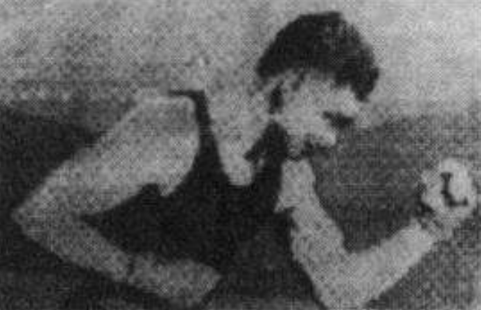
\includegraphics[width=0.7\textwidth]{images/1/halftone.png}
    \caption{Esempio di \textit{halftone printing}.}
\end{figure}

\par
Stampa basata su processo fotografico: proietto luce su una speciale carta sensibile ad essa (stampa ``analogica'', ma i valori possono essere discretizzati, se diverse intensità
di luce rappresentano diversi valori digitali di grigio).
\par
Immagini satellitari (cenno): \textit{1-meter resolution} significa che un pixel dell'immagine copre un quadrato di superificie 1 m\textsuperscript{2}. È una
risoluzione molto alta. Le immagini vengono poi fuse per ottenere un'immagine a bassa risoluzione, ma che copre un'area maggiore.
Se si esprime la risoluzione come \textit{1-meter}, \textit{5-meter}, \textit{50-centimeter} eccetera, più è piccolo il valore di questa ``lunghezza'',
maggiore è la risoluzione: se un'immagine ha risoluzione di 50 centimetri, significa che 1 metro nella realtà è coperto da 2 pixel (alto valore px/m, che è $1/0.5 = 2$),
se la risoluzione è di 5 metri significa che un metro nella realtà è coperto da 0,2 pixel.
\par
Lo spettro elettromagnetico è ampio 16 ordini di grandezza, e in tutto questo intervallo possiamo raccogliere informazione
che può finire in un'immagine. È possibile che un'immagine che vediamo porti contenuti che stanno al di fuori dell'intervallo
della luce a noi visibile, contenuti che sono stati trasposti e portati nell'intervallo a noi visibile, magari senza che ce ne accorgiamo (\hyperref[sec:moving_energy]{ecco un esempio} di come possa succedere).
Analizziamo ora immagini acquisite lungo tutto lo spettro elettromagnetico, partendo dalla luce ad energià più alta.

\subsection{Immagini a raggi gamma (altissima energia)}
Un isotopo radioattivo viene iniettato. Mentre decade, emette positroni (particelle elementari dell'antimateria), e quando un positrone incontra
un elettrone si annichiliscono ed emettono un raggio gamma. Raccogliamo questi raggi e spostiamo l'energia nell'intervallo a noi visibile.
Le zone che attirano più isotopi (in base alla sostanza ``vettore'' che trasporta l'isotopo) sono quelle chiare.
Risultato: proiezione (frontale, posteriore) del corpo umano.

\renewcommand{\thefigure}{1.2}
\begin{figure}[!h]
  \centering
    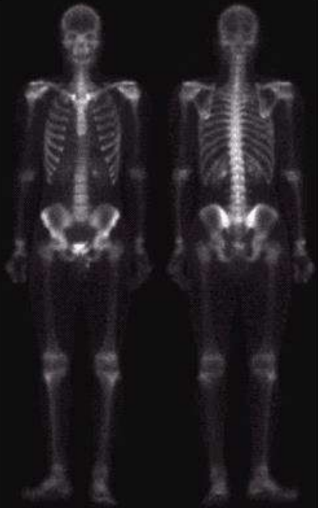
\includegraphics[scale=0.7]{images/1/gamma_ray.png}
    \caption{Immagine a raggi gamma.}
\end{figure}

\subsection{Tomografia a emissione di positroni}
Molto simile. Risultato: una ``fetta'' del corpo umano (sezione ottenuta tagliandolo ad una certa quota).

\subsection{Immagini a raggi X (energia leggermente minore)}
I raggi X sono causati dalla collisione di un elettrone (emesso da un catodo riscaldato) con il nucleo di altri atomi.
Angiografia: inietto liquido di contrasto che è opaco ai raggi X. Si catturano un'immagine con e una senza liquido, poi si confrontano e si capisce dov'è il sangue.

\subsection{Immagini a ultravioletti}
\label{sec:moving_energy}
Usati per analizzare il grano. La trasposizione della luce nell'intervallo di onde a noi visibile è effettuata dall'oggetto stesso (non c'è bisogno di un sensore speciale):
illuminiamo l'oggetto con raggi ultravioletti, e lui rimanda indietro luce visibile a noi.

\subsection{Immagini multispettrali}
Catturate, ad esempio, dal satellite LANDSAT-7. Ogni banda porta informazione di un certo tipo.

\renewcommand{\thefigure}{1.3}
\begin{figure}[!h]
  \centering
    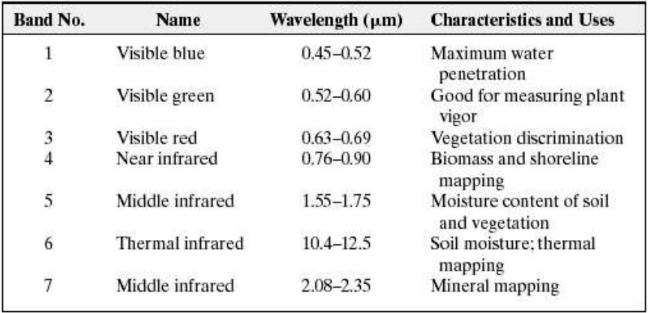
\includegraphics[scale=0.7]{images/1/satellite_bands.png}
    \caption{Bande del satellite LANDSAT-7.}
\end{figure}

In più, c'è la banda pancromatica: non distingue i colori, ma ha larghezza alta! Quindi porta informazioni sull'intensità più dettagliate (cattura meglio i dettagli fini, migliore
precisione spaziale), a scapito delle informazioni sulla presenza o assenza di specifiche frequenze (colori).

\subsection{Immagini a microonde (radar)}
Il radar non cattura luce emessa nello spazio, ma illumina attivamente l'oggetto e poi cattura ciò che torna indietro. La frequenza emessa è bassa, quindi rispetto ai satelliti la risoluzione
è più bassa. Il vantaggio, però, è che è possibile acquisire immagini dallo spazio anche delle zone della Terra coperte da nuvole.

\subsection{Immagini a onde radio (energia molto bassa)}
Mettiamo l'oggetto in un campo magnetico molto alto (diversi Tesla). Aggiungiamo un campo magnetico trasversale periodico. Tutti i nuclei delle sostanze polari si orienteranno
in base al campo costante, ma poi quello periodico li farà oscillare.
Il sistema di acquisizione MRI genera impulsi di campo trasversale che fanno partire
l'oscillazione, si misura il tempo necessario a ogni nucleo per tornare alla posizione di riposo, e da questo si capisce quanto una certa sostanza sia presente in un determinato punto.

\subsection{Immagini a onde acustiche (energia e frequenza bassissime)}
Si piazzano cannoni che sparano aria puntati contro una superficie, si spara e si misura l'eco della superficie, per ottenere informazioni sul sottosuolo. Usate nella ricerca del petrolio.

\subsection{Immagini a onde ``acustiche'' a più alta frequenza}
Per applicazioni mediche, sfruttano onde ``acustiche'' con frequenza nell'ordine dei MHz.

\subsection{Microscopio elettronico a scansione}
Spara fascio di elettroni contro l'oggetto (scansionandolo tutto). Alcuni verranno riflessi in modo diffuso (\textit{backscattering}),
altri verranno assorbiti e genereranno elettroni ``secondari'' che, anch'essi, verranno riflessi diffusamente. Poi si misura la quantità di questi elettroni con appositi trasduttori.

\subsection{Image Fusion Processing for IKONOS 1-m Color Imagery}
L'idea è ovviamente di prendere i dettagli dall'immagine pancromatica e i colori dalle immagini a spettro ristretto.
La risoluzione dei dettagli quindi sarà maggiore di quella dei colori. Questo ben si adatta al sistema visivo
umano, che è meno sensibile alle variazioni di colori rispetto alle variazioni di intensità ($\rightarrow$ non importa che la differenza
tra due colori quasi identici venga rilevata, tanto noi non la vedremmo comunque).
Questo fatto viene sfruttato in tutti gli ambiti di fotografia/produzione video, per evitare di trasmettere informazione che noi non saremmo in grado di apprezzare.
\par
Tra le varie tecniche per fondere l'immagine pancromatica e quelle a spettro ristretto, la prima da considerare è la metodologia IHS (\textit{intensity hue saturation}).
Si sommano tra loro (ipotizzo) le immagini a spettro ristretto, poi l'immagine risultante viene trasformata dal dominio RGB a quello IHS (intensità, tinta, saturazione).
La sua intensità, che sarà $I = (R+G+B)/3$, viene sostituita dal valore d'intensità dell'immagine pancromatica nello stesso punto (quindi bisogna ingrandire le immagini
a spettro ristretto, in modo da avere una corrispondenza 1 a 1 tra i loro pixel e quelli dell'immagine pancromatica). Poi ci si sposta di nuovo nel dominio RGB per ottenere l'immagine finale.
\par
La seconda tecnica è basata sull'analisi delle componenti principali (PCA). Si uniscono (sommandole) le immagini a spettro ristretto, poi si estraggono le loro prime tre componenti
principali, la prima viene sostituita dal valore dell'immagine pancromatica nel pixel corrispondente, e poi si torna nello spazio RGB.

\subsection{Satelliti LANDSAT 8 e 9}
Ci sono più sensori e viene fornita informazione più precisa (risoluzione dell'intensità di 12 b/px) rispetto all'IKONOS.
Non ci sono componenti mobili: nelle generazioni precedenti c'era uno specchio che si muoveva per scansionare
il terreno, e dirigeva la luce verso uno dei sensori. Ora c'è una fila di 7000 sensori che lavorano in parallelo.

\newpage

\section{Il sistema visivo umano}
Coni ($10^6$): per la percezione dei colori, concentrati sulla fovea. Esistono coni di 3 tipi (sensibili a rosso, verde e blu).
Questo è il motivo della bassa sensibilità alle piccole variazioni dei colori (la curva di risposta di ogni cono è molto ``stretta'' e cala velocemente).
\textit{L-cone}: cono sensibile al rosso (lunghezza d'onda grande). \textit{M-cone}: cono sensibile al verde (media lunghezza d'onda). \textit{S-cone}: cono sensibile al blu (lunghezza d'onda piccola).
La visione permessa dai coni è quella \textbf{fotopica}.
\par
Bastoncelli ($10^8$): usati quando c'è poca luce, sono molto più sensibili dei coni. La visione permessa dai bastoncelli si chiama \textbf{scotopica}.
Sono pancromatici (combinano tutti i colori insieme, non danno informazioni sui colori).
\par
Il nervo ottico ha solo $10^6$ fibre, quindi l'occhio effettua compressione.
Le cellule orizzontali fanno interagire l'informazione tra diversi recettori, anche molto lontani, e così avviene la compressione.
Nella foveola (parte interna della fovea) non ci sono vasi sanguigni, che potrebbero ostacolare la luce. Non ci sono neanche le
cellule-processori.
\par
\textbf{Metamerismo}: diverse distribuzioni spettrali della luce possono stimolare allo stesso modo i tre tipi
di coni e risultare indistinguibili. Ad esempio, se vediamo un punto verde, potrebbe derivare da una sorgente che emette luce con spettro
molto stretto e centrato su una frequenza del verde, oppure una sorgente che emette luce ad ampissimo spettro.
Questo non è uno svantaggio, anzi, noi lo sfruttiamo negli schermi, per produrre tanti colori combinando in diversi modi soltanto una frequenza di rosso, una di verde e una di blu.
\par
Ecco i grafici della sensibilità, misurata in lumen/W, di coni e bastoncelli. I valori sono normalizzati rispetto alla massima sensibilità ottenibile,
perché altrimenti dovremmo misurare, per ogni recettore, il valore esatto della sua risposta (impossibile e inutile).

\newpage
\renewcommand{\thefigure}{2.1}
\begin{figure}[!h]
  \centering
    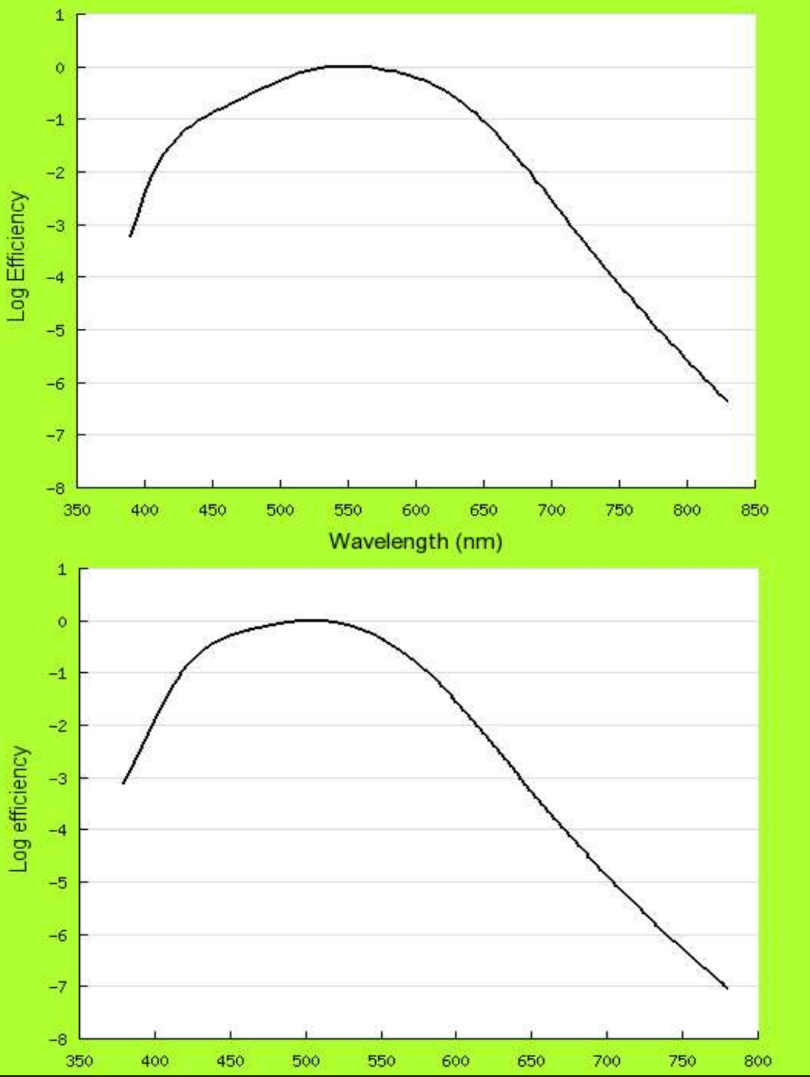
\includegraphics[scale=0.4]{images/2/cones_rods_sensitivity.png}
    \caption{Risposte della visione fotopica e scotopica.}
\end{figure}

\subsection{Radiometria}
\begin{itemize}
    \item Energia radiante [$J$]: poco interessante per noi, è solo il valore assoluto dell'energia della luce, mentre a noi interessano di più le sue variazioni.
    \item Flusso o potenza radiante [$W$]: energia emessa o ricevuta per unità di tempo.
    \item Densità del flusso radiante [$W/m^2$]: flusso per unità di superficie. Si definisce irradianza se entrante, eccitanza radiante se uscente.
    \item Intensità radiante [$W/sr$]: flusso di una sorgente puntiforme per unità di angolo solido (1 steradiante).
    \item Radianza [$W/(m^2 \cdot sr)$]: flusso emesso da una sorgente puntiforme, per unità di angolo solido, e per unità di superficie colpita.
\end{itemize}

\subsection{Fotometria}
Come passare dal dominio della radiometria (luce studiata come entità fisica) a quello della fotometria (luce studiata per come la percepiamo)?
Bisogna conoscere la risposta della visione fotopica dell'occhio, descritta da una funzione chiamata
\textit{funzione di efficienza luminosa spettrale}, $V(\lambda)$.
Una quantità radiometrica $\Phi(\lambda)$ viene trasformata nella relativa quantià fotometrica $\Phi_V$ in questo modo:
\[\Phi_V = \int_\lambda \Phi(\lambda) V(\lambda) \,d\lambda \]
Quantità fotometriche:
\begin{itemize}
    \item energia luminosa [$lm \cdot s$]: come prima, poco interessante, a tal punto che l'unità di misura viene appositamente appesantita moltiplicandoci l'unità di tempo, così dopo abbiamo un'unità
    di misura più semplice per il flusso;
    \item flusso/potenza luminoso/a [$lm$]: il flusso dell'energia luminosa, tenendo solo i contributi delle frequenze visibili, per unità di tempo;
    \item \textbf{densità di flusso luminoso} [$lx \coloneqq lm / m^2$]: flusso per unità di superficie. Si definisce illuminanza se entrante, eccitanza luminosa se uscente;
    \item intensità luminosa [$cd \coloneqq lm / sr$]: flusso emesso da sorgente puntiforme per unità di angolo solido;
    \item \textbf{luminanza} [$nit \coloneqq cd / m^2$]: intensità per unità di superficie colpita.
\end{itemize}

Legge di Lambert: l'illuminanza di una superficie è proporzionale al coseno dell'angolo tra la normale alla superficie colpita e la direzione dei raggi di luce entranti.

\newpage
\renewcommand{\thefigure}{2.2}
\begin{figure}[!h]
  \centering
    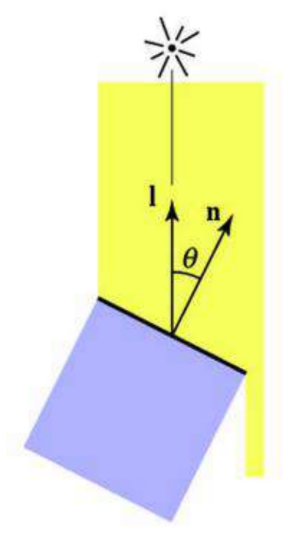
\includegraphics[scale=0.4]{images/2/lamberts_law.png}
    \caption{Legge di Lambert: l'illuminanza è proporzionale a $cos\theta$.}
\end{figure}


\subsection{Polarizzazione della luce}
In ambiente aperto, la luce è un'onda con ampiezza e inclinazione delle oscillazioni del campo elettromagnetico molto variabili.
\par
Analizziamo solo una delle componenti della luce, ovvero il campo elettrico. La luce si dice ``polarizzata'' (in diversi modi) se la punta del vettore del campo elettrico $\overrightarrow{E}$
che si propaga nella direzione dell'asse $z$ segue delle linee ben precise.
\newline
Polarizzazione lineare: si ha se le componenti $\overrightarrow{E_x}$ ed $\overrightarrow{E_y}$ del campo elettrico che si propaga lungo l'asse $z$
sono in fase e di uguale ampiezza. Il vettore $\overrightarrow{E}$ quindi giacerà sempre sulla stessa diagonale, e varierà solo in modulo. La sua punta percorrerà su e giù questa diagonale.

\renewcommand{\thefigure}{2.3}
\begin{figure}[!h]
  \centering
    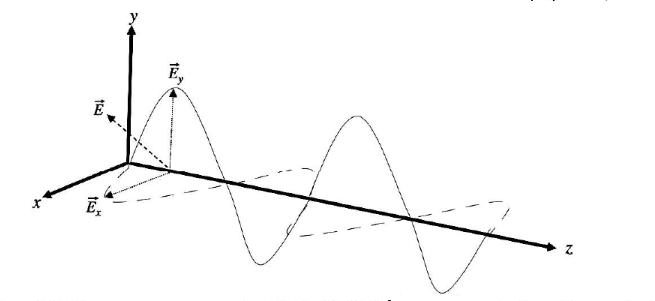
\includegraphics[scale=0.6]{images/2/linear_polarization.png}
    \caption{Polarizzazione lineare.}
\end{figure}

Se invece le componenti sono sfasate di $\pi /2$, ma di uguale ampiezza, la polarizzazione è circolare.
Entrambe queste polarizzazioni sono casi specifici della polarizzazione ellittica,
che è il caso generale, che comprende sfasamenti e differenze di ampiezza arbitrari.

\renewcommand{\thefigure}{2.4}
\begin{figure}[!h]
  \centering
    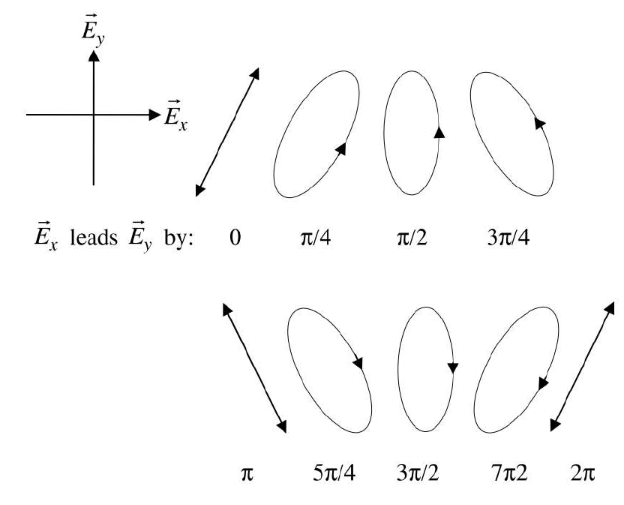
\includegraphics[scale=0.6]{images/2/elliptic_polarization.png}
    \caption{Polarizzazione ellittica.}
\end{figure}

\subsection{Percezione visiva}

\renewcommand{\thefigure}{2.5}
\begin{figure}[!h]
  \centering
    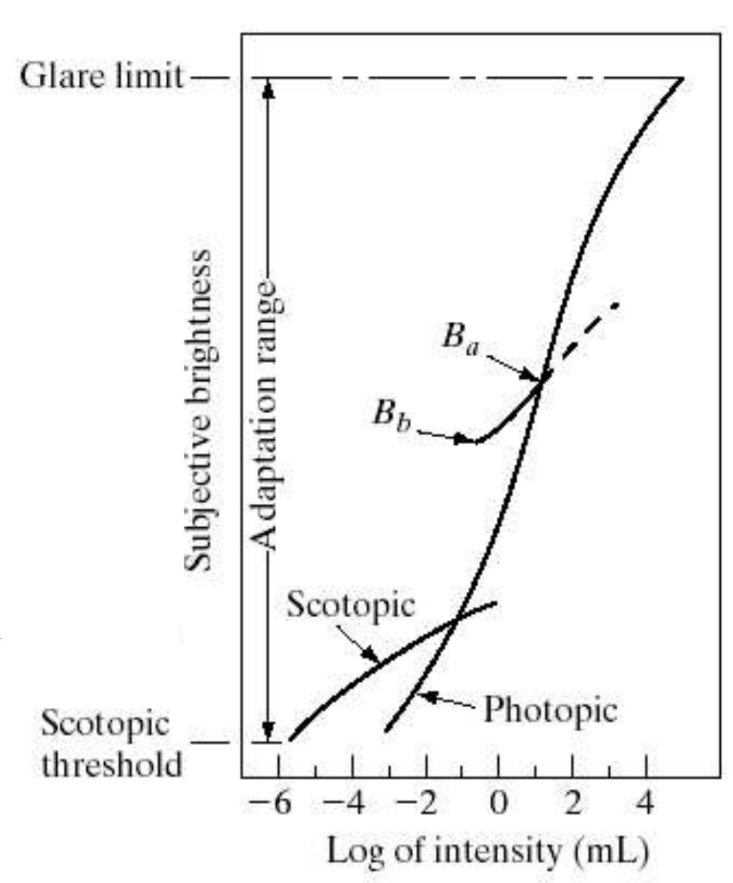
\includegraphics[scale=0.3]{images/2/response_stimulus.png}
    \caption{Risposta ad uno stimolo luminoso.}
\end{figure}

Il grafico mostra la percezione soggettiva di uno stimolo luminoso. La zona di interesse sull'asse $y$ va dalla soglia della visione scotopica
(sotto la quale non vediamo nulla) al limite di abbagliamento (oltre il quale la luce ci acceca e non distinguiamo nulla).
Si nota che, in questo intervallo di interesse, sull'asse $x$ sono compresi 10 ordini di grandezza (lasciamo perdere l'unità di misura non standard):
siamo quindi in grado di vedere in un intervallo di intensità luminose davvero ampio. La percezione data dalla visione fotopica sembra avere forma sigmoidale, ma non essendo una quantità misurabile
con precisione, non è detto sia esattamente così.
\par
Supponiamo di esserci adattati ad una certa intensità luminosa presente nell'ambiente. Sappiamo per esperienza che è facile
adattarsi ad un aumento improvviso di intensità, mentre adattarsi ad un calo richiede un po' di tempo. Questo fenomeno è descritto
dalla piccola curva contenente i punti $B_a$ e $B_b$: fissato $B_a$ come punto di adattamento attuale, se la luminosità cala
repentinamente, la nostra percezione inizialmente seguirà la curva fino al punto $B_b$, al di sotto della quale vedremo tutto nero
(fino a quando non ci assesteremo su un nuovo punto di adattamento). Se invece la luminosità aumenta, siamo così veloci ad adattarci
che invece di seguire la porzione tratteggiata della curva, risaliamo praticamente immediatamente la sigmoide principale e ci assestiamo sul nuovo punto di adattamento.

\subsection{JND ed esperimenti relativi}
Esperimento 1: uno schermo è illuminato ad una certa intensità $I$. In una piccola regione al centro, ad intermittenza, viene incrementata
l'intensità di $\Delta I$. L'immagine risultante è dinamica (varia nel tempo).
\newline
Esperimento 2: uno schermo è illuminato ad una certa intensità $I$. In una piccola regione al centro, si modifica l'intensità
applicando una variazione sinusoidale orizzontale di ampiezza $\Delta I$.  L'immagine risultante è statica (la variazione sinusoidale è fissa, non si muove).
\par
Qual è il minimo valore di $\Delta I$ che produce un cambiamento appena rilevabile (\textit{just noticeable difference}, JND)? Dipenderà da diversi
fattori e sarà diverso per i due esperimenti. Chiamiamolo $\Delta I_c$ (\textbf{soglia di contrasto}) in entrambi i casi.
Il \textbf{rapporto di Weber} è $\frac{\Delta I_c}{I}$. La legge empirica di Weber dice che questo rapporto è costante, ma in realtà non lo è sempre.

\newpage
\renewcommand{\thefigure}{2.6}
\begin{figure}[!h]
  \centering
    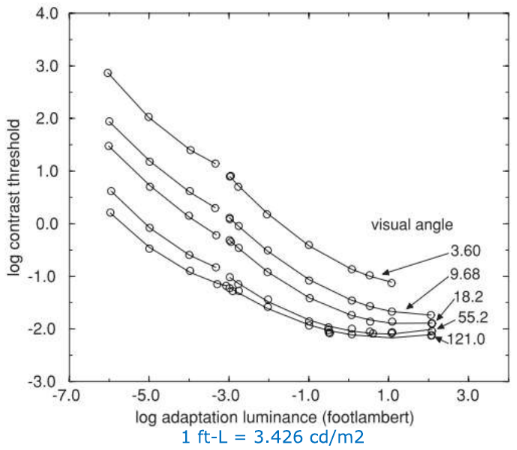
\includegraphics[scale=0.8]{images/2/contrast_threshold.png}
    \caption{Soglia di contrasto al variare di $I$.}
\end{figure}

Dal grafico si nota che quando $I$ è bassa, serve un $\Delta I_c$ grande per notare una differenza. Ma non ci interessa, questo riguarda i bastoncelli.
All'aumentare di $I$, entrano in gioco i coni e $\Delta I_c$ si stabilizza (vale la legge empirica di Weber).

\subsection{Progettazione di uno schermo}
Sulla base di quanto visto fin'ora, quanto precisamente dobbiamo quantizzare la luminosità di uno schermo?
Per scoprirlo, usiamo il modello di Naka-Rushton per descrivere la risposta dei nostri fotorecettori. $P()$ è la risposta dei recettori,
$L$ è la luminanza dello schermo (la quantità sull'asse orizzontale), $S$ è una quantità che descrive in qualche modo il nostro punto di adattamento (seleziona quale sigmoide seguire).
\[P(L, S) = \frac{L}{L+S}\]
Ne consegue che quando $L = S$, allora $P(L,S) = 0.5$, e lì intorno la risposta è lineare, proporzionale a $L$ (cioè, intorno al punto di adattamento il comportamento dell'occhio
è molto regolare: la variazione nella risposta è proporzionale alla variazione dello stimolo).
\newline
L'insieme immagine di $P()$ è $[0,1]$ perché ci fa comodo così - tanto non è una quantità misurabile precisamente!

\newpage
\renewcommand{\thefigure}{2.7}
\begin{figure}[!h]
  \centering
    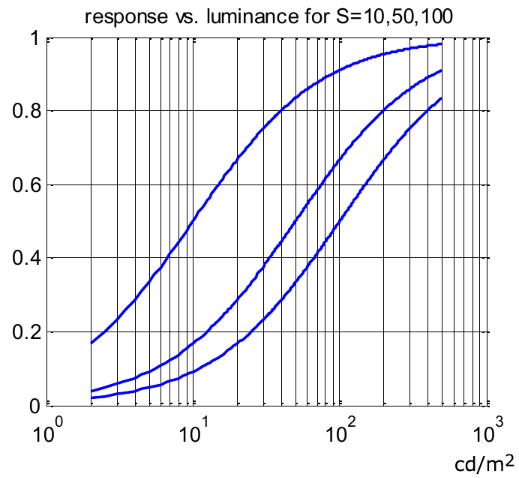
\includegraphics[scale=0.5]{images/2/naka_rushton.png}
    \caption{Risposta dei nostri recettori secondo il modello di Naka-Rushton.}
\end{figure}

\par
Siamo però interessati alla risposta dell'occhio ad una variazione di intensità, perché sono le variazioni a portare informazione. Consideriamo allora la risposta al contrasto normalizzata.
\[ncr(L,S) = \frac{dP}{(dL/L)} = \frac{L\cdot S}{(L+S)^2}\]
Questa sarebbe la derivata di $P()$ non rispetto ad una variazione assoluta di $L$, ma rispetto ad una sua variazione relativa $\frac{dL}{L}$ (intuitivamente, una derivata ``più complicata'').

\renewcommand{\thefigure}{2.8}
\begin{figure}[!h]
  \centering
    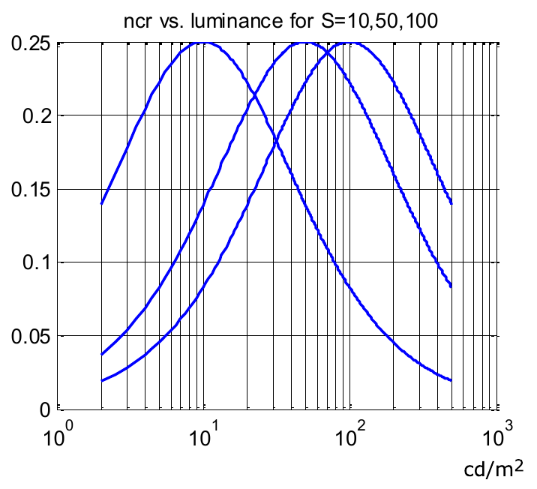
\includegraphics[scale=0.5]{images/2/ncr.png}
    \caption{Risposta al contrasto normalizzata.}
\end{figure}

Questa risposta al contrasto ha il suo massimo in $L=S$, il che significa che la nostra sensibilità alle variazioni di intensità
è massima intorno al punto di adattamento (proprio quello che abbiamo detto poco fa). Massima sensibilità significa minima soglia di contrasto, come ora
vediamo esaminando la soglia di contrasto normalizzata (grafico più o meno identico al precedente, ma ribaltato)
\[nct(L,S) = ncr(L,S)^{-1}.\]
Questa funzione, però, ha dei valori che non significano nulla, poiché sono semplicemente l'inverso dei valori della $ncr()$, i quali, a loro volta, derivavano dall'intervallo arbitrario
scelto per i valori di $P()$.
Dobbiamo denormalizzarli, cioè riportarli a valori significativi e fondati sulla realtà, e lo possiamo fare grazie agli esperimenti di Barten e Ferwerda: dobbiamo portare i minimi
delle curve ribaltate al valore della soglia di contrasto ottimale, $cto$, da loro individuato. Nota: $cto$ è un numero puro.
Poiché i minimi delle curve attualmente hanno ordinata pari a $4 = 0.25^{-1}$, dobbiamo prima dividere per 4 e poi moltiplicare per $cto$. Otteniamo quindi
\[ct(L,S,cto) = \frac{nct(L,S)}{4} \cdot cto\]

\renewcommand{\thefigure}{2.9}
\begin{figure}[!h]
  \centering
    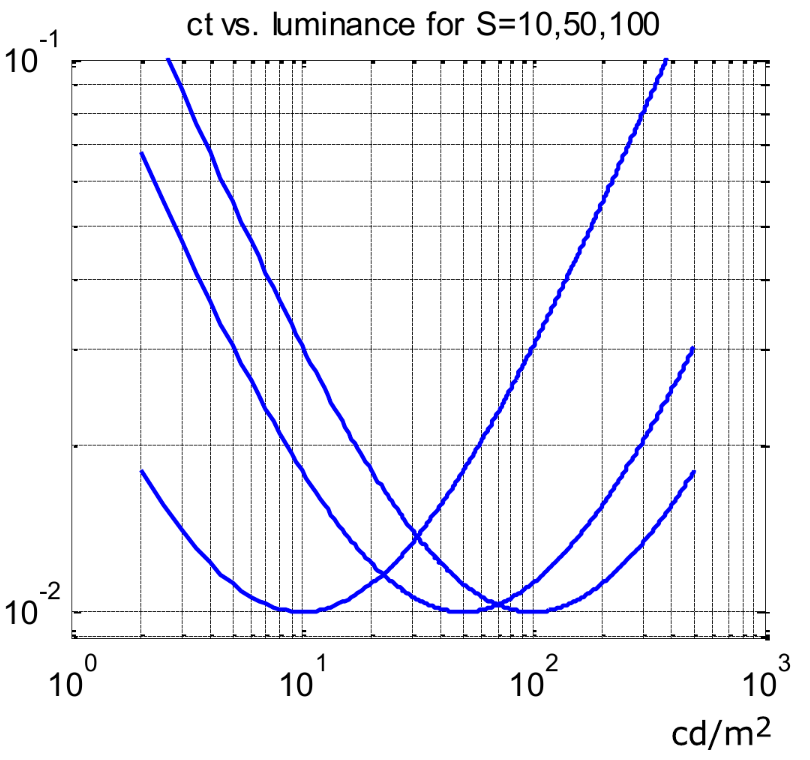
\includegraphics[scale=0.5]{images/2/ct.png}
    \caption{Soglia di contrasto denormalizzata (secondo Barten).}
\end{figure}

$cto$ qui va ad aggiungersi ai parametri della funzione, poiché dipende dall'esperimento (Barten dice che $cto = 0.01$, Ferwerda dice che $cto = 0.1$). A questo punto abbiamo una funzione
$ct()$ che dice che si ha la soglia di contrasto ottimale (cioè più bassa possibile) quando la luminanza dello schermo coincide con il nostro punto di adattamento.
\par
Definiamo $L_{max}$ la massima luminanza di uno schermo, $L_{min}$ la minima, ed $L_i$ i valori intermedi: minore è $i$, maggiore
è la luminanza. La scala dei livelli di luminanza in ordine decrescente è quindi
\[L_{max}, L_1, L_2, L_3, ..., L_{min}\]
Per quanto detto prima, sappiamo che
\[
cto = \frac{\Delta I_c}{I}  = \frac{(L_{i-1}-L_i)}{L_i}
= \frac{L_{i-1}}{L_i} - 1,
\]
cioè
\[1+cto = \frac{L_{i-1}}{L_i}\]
Scrivendo le N istanze di questa equazione che servono ad andare dal vedere $L_{max}$ al numeratore fino a $L_{min}$ al denominatore, e moltiplicandole poi tra di loro, si ottiene
\[
(1+cto)^N = \frac{L_{max}}{\cancel{L_1}}\cdot \frac{\cancel{L_1}}{\cancel{L_2}} \cdot
\frac{\cancel{L_2}}{\cancel{L_3}} \cdot ... \cdot \frac{\cancel{L_{N-1}}}{L_{min}} = \frac{L_{max}}{L_{min}}.
\]
Si cerca poi il massimo valore di N tale che
\[
(1+cto)^N \leq \frac{L_{max}}{L_{min}}.
\]
Questo sarà il numero di JND che lo schermo è in grado di visualizzare, cioè il numero di livelli di luminanza da implementare, nell'ipotesi che il nostro occhio si adatti
a ciascun livello di luminanza in tempo zero (caso ideale di adattamento variabile).
\par
Bisogna però annorare il caso, più realistico, di adattamento fisso, in cui l'occhio non ha il tempo di adattarsi al nuovo livello
di luminanza. In questo caso non possiamo usare $cto$, perché la soglia di contrasto per permetterci di cogliere una differenza
sarà più alta. La soglia da usare dipenderà da ciascun livello, e la possiamo indicare con $ct(L(i))$.
In questo caso, il numero di JND producibili dallo schermo sarà ben inferiore, e dipenderà dallo stato di adattamento. Il significato di questo grafico è: se siamo adattati ad un valore di luminanza
medio, il numero di JND sarà relativamente alto (riusciremo a distinguere differenze tra coppie di livelli di luminanza bassi o alti). Se invece siamo adattati a un livello di luminanza alto,
il numero di JND sarà piccolo, perché non saremo in grado di percepire le differenze tra livelli di luminanza bassi (vediamo tutto indistinguibilmente nero).

\newpage
\renewcommand{\thefigure}{2.10}
\begin{figure}[!h]
  \centering
    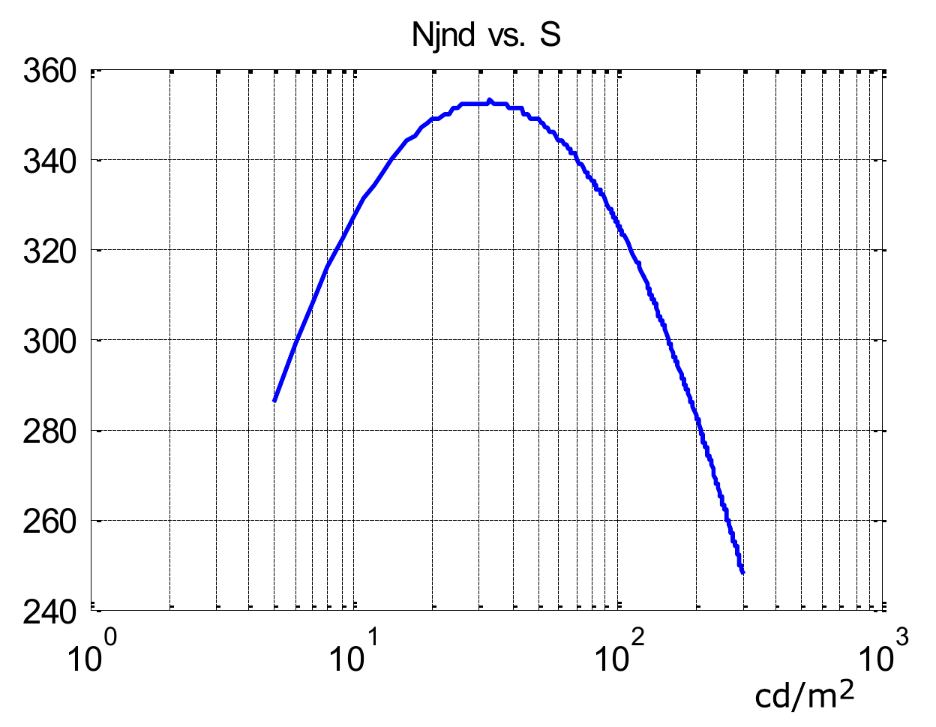
\includegraphics[scale=0.5]{images/2/jnd_fixed.png}
    \caption{Numero di JND in funzione del punto di adattamento.}
\end{figure}


Nel prossimo grafico usiamo $[2, 500] \,cd/m^2\, (nit)$ come intervallo d'interesse per la luminanza dello schermo, perché questo
è l'intervallo usato negli schermi di macchinari medici, dove la qualità richiesta è elevata, quindi le loro proprietà rappresentano bene come un buono schermo debba essere.
Nel grafico, sull'asse $y$ c'è la soglia di contrasto richiesta per una JND.
La curva A rappresenta la soglia di contrasto necessaria nel caso di stato di adattamento variabile, che ovviamente è sempre inferiore,
come detto prima, a quella necessaria nello stato di adattamento fisso (curva B).

\newpage
\renewcommand{\thefigure}{2.11}
\begin{figure}[!h]
  \centering
    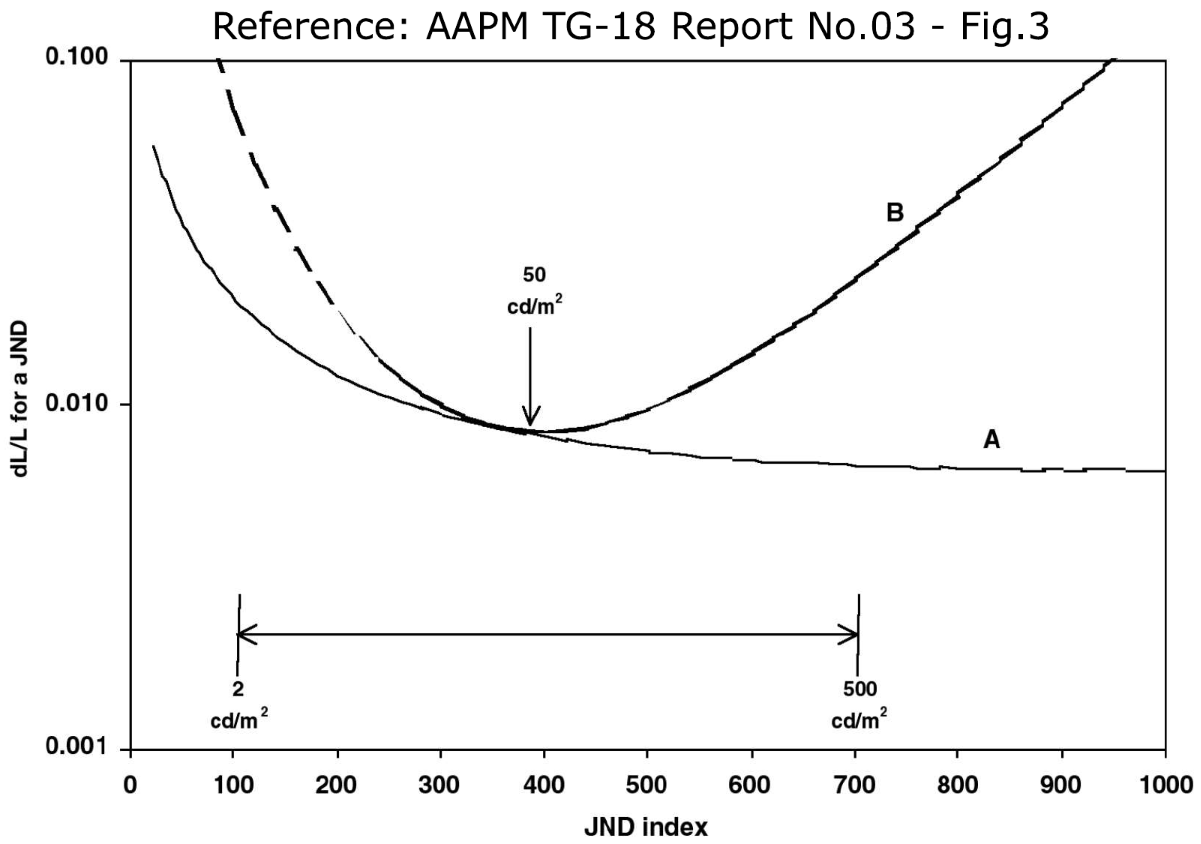
\includegraphics[scale=0.38]{images/2/fixed_vs_varying.png}
    \caption{Soglia di contrasto per adattamento fisso (B) e variabile (A).}
\end{figure}

\subsection{Effetti della luce ambientale}

\renewcommand{\thefigure}{2.12}
\begin{figure}[!h]
  \centering
    
\includegraphics[scale=0.3]{images/2/circles.png}
    \caption{Il punto di adattamento indotto dall'anello influenza la percezione dei dettagli.}
\end{figure}

La trama grigia, con i suoi dettagli, dovrebbe essere meglio visibile nel caso di mezzo, dove è circondata da un anello grigio, che nei casi di destra e sinistra.
Questo perché i cerchi bianchi e neri spostano il punto di adattamento verso le alte e basse luminanze, rispettivamente, e come ormai è chiaro, noi siamo
in grado di cogliere al meglio le differenze cromatiche (e quindi i dettagli) solo in un intorno del punto di adattamento.
\par
La nostra percezione inoltre è influenzata dalla luce ambientale, che viene riflessa dallo schermo. In uno schermo di un computer il riflesso va evitato, poiché lo schermo produce luce di suo.
Per un telo da proiettore, dove l'idea è proprio quella di mostrare immagini riflettendo la luce che proviene dal proiettore,
bisognerebbe minimizzare la luce ambientale: questo è il motivo per cui al cinema c'è buio.
In base al tipo di superficie su cui la luce ambientale incide, possiamo avere tre effetti.
\begin{enumerate}
    \item Riflessione speculare: l'angolo di riflessione è uguale a quello di incidenza.
    \item Riflessione diffusa (\textit{haze}): il raggio viene riflesso a più angoli, leggermente diversi da quello d'incidenza.
    \item Riflessione diffusa uniforme (di Lambert): come quella diffusa, ma in tutte le possibili direzioni a 180°.
    Quasi tutti gli schermi sono di questo tipo. Quelli più scadenti possono avere anche riflessione speculare.
\end{enumerate}
\par
Vediamo come la riflessione influenza il numero di JND ottenibili in uno schermo. Ipotizziamo che il nostro schermo abbia
un coefficiente di riflessione diffusa $R_d = 0,02 \; sr^{-1}$. Questo valore è il rapporto tra l'energia del raggio
riflesso e quella del raggio incidente. Questo è un valore molto basso, lo schermo è di ottima qualità.
Nella stanza abbiamo $I = 30$ lux (è molto buio). Quant'è la luce riflessa ($Lamb$)?
$Lamb = I \cdot R_d = 0,6\; \text{cd/m}^2 = 0.6$ nit.
Questo valore si aggiunge come un offset alla minima e massima luminanza ottenibile dallo schermo: l'intervallo dinamico effettivo diventa
\[\frac{L_{max}+Lamb}{L_{min}+Lamb}\]
La poca luce riflessa dallo schermo incide comunque negativamente sulle JND ottenibili (basta considerare che questa frazione sarà sensibilmente minore di $L_{max}/L_{min}$
anche per valori piuttosto piccoli di $Lamb$, diminuisce dunque l'intervallo dinamico dello schermo).

\newpage

\subsection{Funzione di sensibilità al contrasto}

\renewcommand{\thefigure}{2.13}
\begin{figure}[!h]
  \centering
    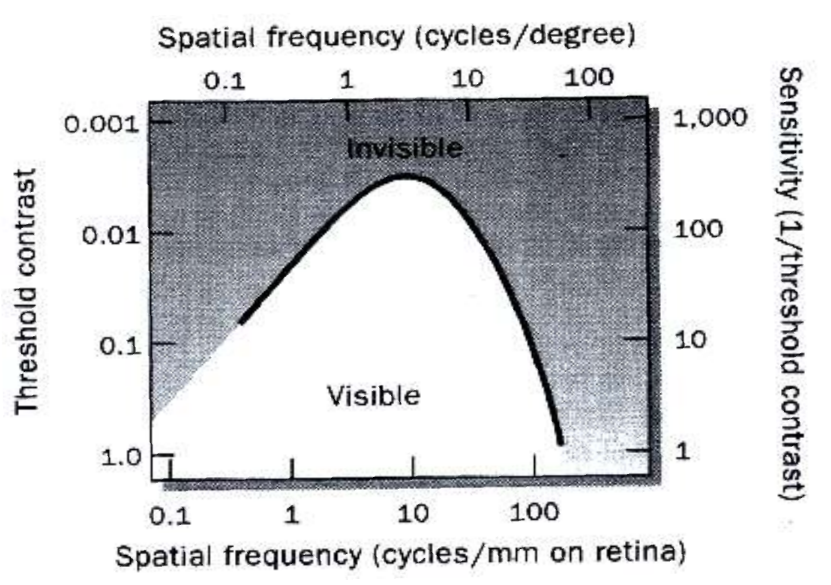
\includegraphics[scale=0.5]{images/2/sensitivity_vs_spatial_freq.png}
    \caption{Sensibilità al variare della frequenza spaziale.}
\end{figure}

Notare che l'asse $y$ di sinistra è invertito! In parole povere, se la frequenza spaziale dello stimolo è molto alta o molto bassa,
dev'essere piuttosto alto il contrasto tra le creste e le pance della sinusoide affinché noi possiamo notarle (abbiamo cioè minore sensibilità, serve che le creste siano molto chiare e
le pance molto scure). Se invece la frequenza spaziale è moderata, riusciamo a cogliere differenze anche piuttosto lievi.

\renewcommand{\thefigure}{2.14}
\begin{figure}[!h]
  \centering
    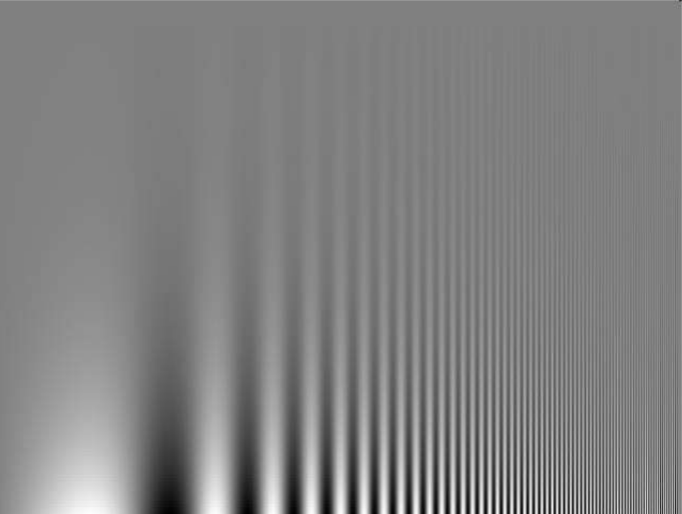
\includegraphics[scale=0.4]{images/2/spatial_sinusoid.png}
    \caption{Sinusoide con frequenza spaziale crescente.}
\end{figure}

Questa immagine spiega in termini pratici lo stesso fenomeno: al centro, vediamo le oscillazioni fino a molto in alto, mentre ai lati a metà dell'altezza dell'immagine
sono già del tutto invisibili. La zona in cui le oscillazioni sono visibili ha un confine a forma di campana, piuttosto simile a quello del grafico precedente.
\par
Ovviamente il tutto dipende anche dalla quantità di luce che incide sulla retina (misurata in $troland$). Se ce n'è poca, la sensibilità è molto ridotta.

\renewcommand{\thefigure}{2.15}
\begin{figure}[!h]
  \centering
    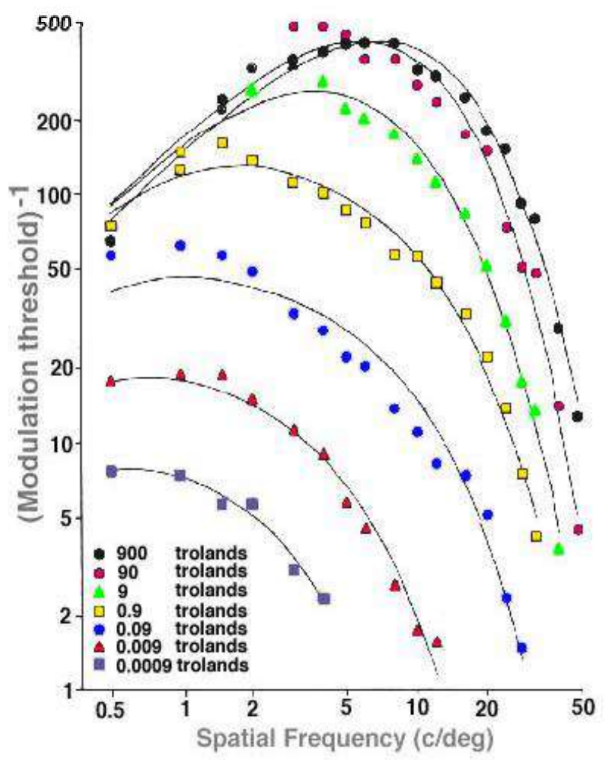
\includegraphics[scale=0.4]{images/2/spatial_freq_trolands.png}
    \caption{Sensitività al contrasto per diverse quantità di luce che raggiunge la retina.}
\end{figure}

\newpage

\subsection{Illusioni ottiche}

\renewcommand{\thefigure}{2.16}
\begin{figure}[!h]
  \centering
    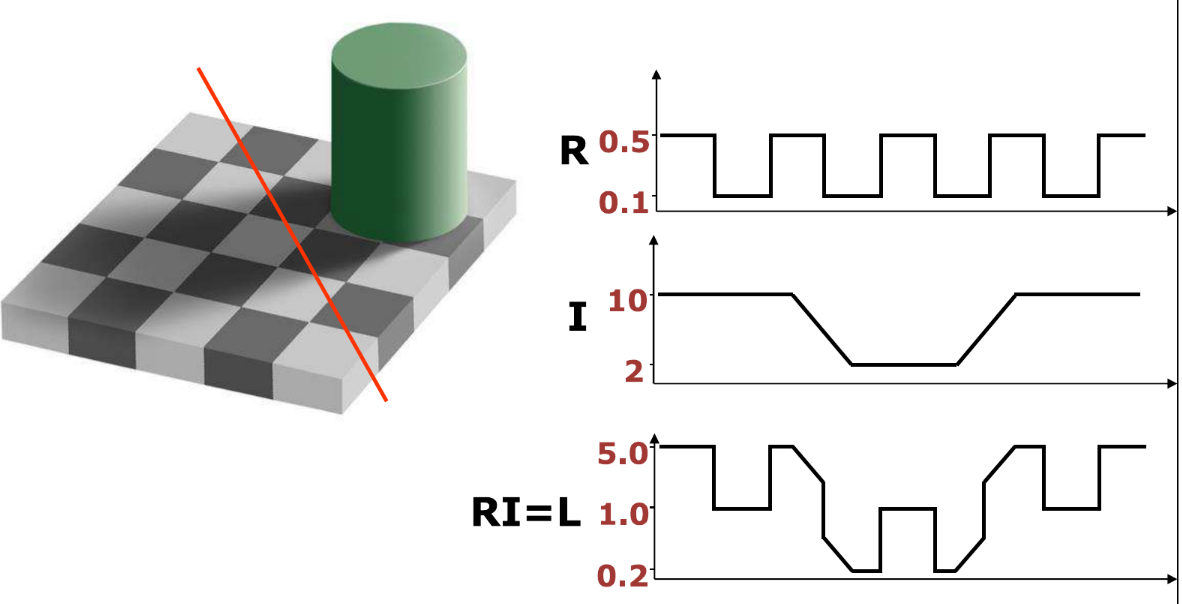
\includegraphics[scale=0.4]{images/2/chessboard.png}
    \caption{Illusione ottica della scacchiera.}
\end{figure}

Qui il nostro cervello riesce a scartare l'informazione sull'illuminazione ``assoluta'' della scena, e a dare importanza solo alla luce che
viene riflessa dagli oggetti della scena, che è ciò a cui siamo interessati per percepire davvero bene la scena.
$L=I \cdot R$, il nostro occhio vede $L$, scarta $I$ (che dice quali zone sono in ombra) e mantiene solo R (ed è quindi in grado di ricostruire i colori fedelmente anche nelle zone di ombra,
perché fa finta che non siano in ombra, praticamente).
\par
L'effetto Mach invece ci fa apparire ogni banda grigia leggermente più chiara a sinistra (dove tocca una banda più scura), e leggermente più scura a destra (dove ne tocca
una più chiara).

\newpage
\renewcommand{\thefigure}{2.17}
\begin{figure}[!h]
  \centering
    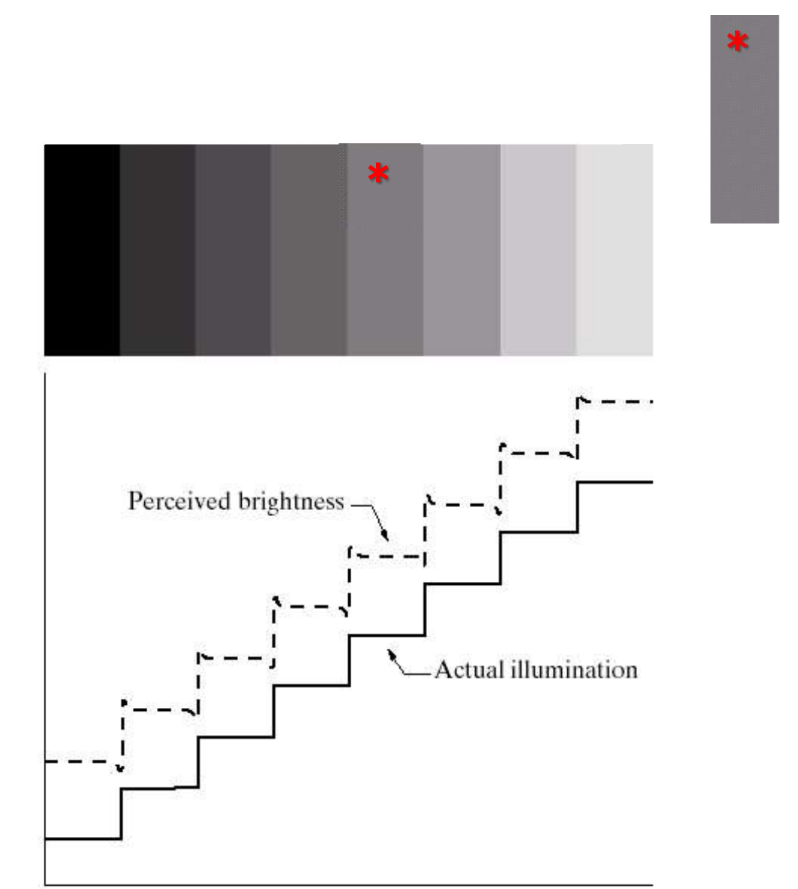
\includegraphics[scale=0.4]{images/2/mach_band.png}
    \caption{Effetto Mach.}
\end{figure}


\subsection{\textit{Shape from shading}}
È uno strumento di \textit{computer vision} che permette di ricostruire la struttura tridimensionale di un oggetto da una sola acquisizione, se due ipotesi sono rispettate:
\begin{enumerate}
\item è nota la posizione della sorgente di luce;
\item l'oggetto è omogeneo (un unico colore, differenze date soltanto dalle zone che vanno più o meno in ombra).
\end{enumerate}
Molto difficile che un oggetto reale sia omogeneo, quindi servono più immagini catturate con diverse condizioni di illuminazione.
\par
Albedo: quantità di luce riflessa da un singolo punto di un oggetto o dall'oggetto intero, cioè come vedremmo l'oggetto se l'illuminazione fosse diffusa (non proveniente da un singolo punto).

\subsection{Percezione della profondità e visione binoculare}
La visione binoculare, fortunatamente, non è il solo strumento che abbiamo per percepire la profondità di una scena. Ce ne sono anche altri, che sono d'aiuto
perché per alcune distanze, la visione binoculare non funziona molto bene. Questi altri strumenti sono:
\begin{itemize}
\item le dimensoni degli oggetti noti;
\item la sfocatura (anche introdotta artificialmente);
\item il movimento.
\end{itemize}

\renewcommand{\thefigure}{2.18}
\begin{figure}[!h]
  \centering
    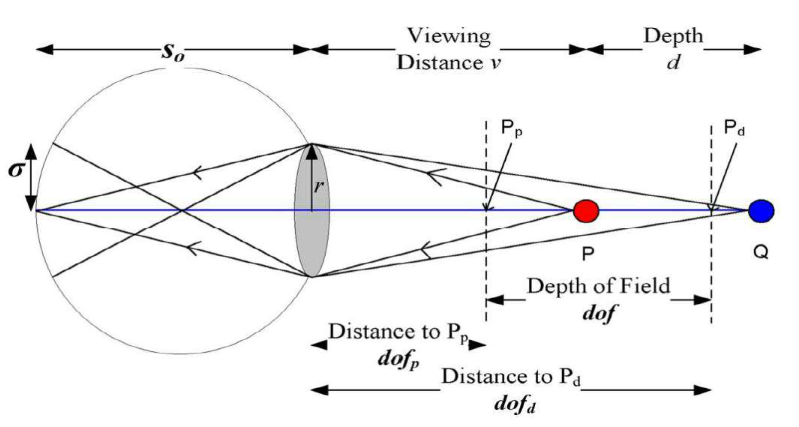
\includegraphics[scale=0.5]{images/2/confusion.png}
    \caption{Profondità di campo e cerchio di confusione.}
\end{figure}

Il punto rosso è posto ad una distanza
adeguata dal nostro occhio, quindi viene proiettato sulla retina come un punto.
Il punto blu invece si trova troppo lontano, allora viene proiettato sulla retina come
un cerchio sfocato (\textit{circle of confusion}). La profondità di campo
(\textit{depth of field}) è l'intervallo di distanza all'interno del quale un punto
deve essere posto affinché la dimensione del circolo di confusione sia trascurabile.

\renewcommand{\thefigure}{2.19}
\begin{figure}[!h]
  \centering
    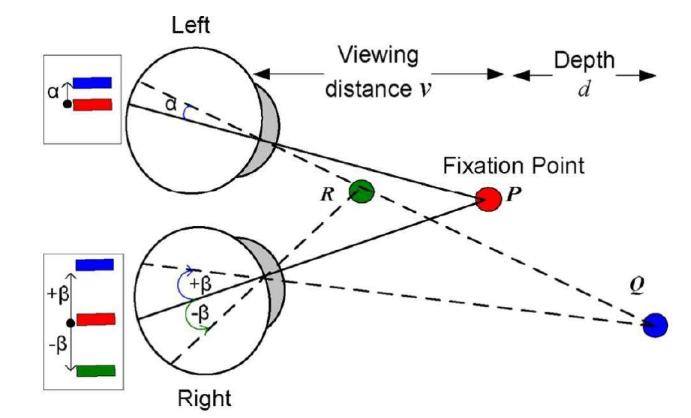
\includegraphics[scale=0.5]{images/2/parallax.png}
    \caption{Visione binoculare.}
\end{figure}

Visione binoculare: gli occhi fissano un punto P (\textit{fixation point}), che produce un'immagine sulla retina. Durante il movimento, il cervello ricostruisce le distanze P-Q e P-R grazie alle
informazioni sugli angoli tra le due immagini riprodotte sulla retina.

\newpage

\section{Acquisizione}
\subsection{Fotodiodi}
Sono sensibili alla luce, e normalmente polarizzati inversamente, cioè il polo positivo
della batteria è collegato al lato \textit{n} della giunzione, e viceversa.

\renewcommand{\thefigure}{3.1}
\begin{figure}[!h]
  \centering
    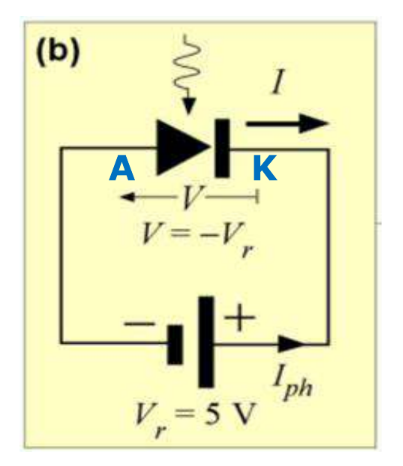
\includegraphics[scale=0.4]{images/3/reverse_bias.png}
    \caption{Polarizzazione inversa di un fotodiodo.}
\end{figure}

Il lato \textit{n} della giunzione è molto più ampio di quello \textit{p}, cioè la parte \textit{p} è altamente drogata,
così da poter essere sottile, e di conseguenza la zona di svuotamento è molto più estesa sul lato \textit{n}.
L'elettrodo dal lato \textit{p} (l'anodo) ha un buco per permettere l'ingresso della luce.

\renewcommand{\thefigure}{3.2}
\begin{figure}[!h]
  \centering
    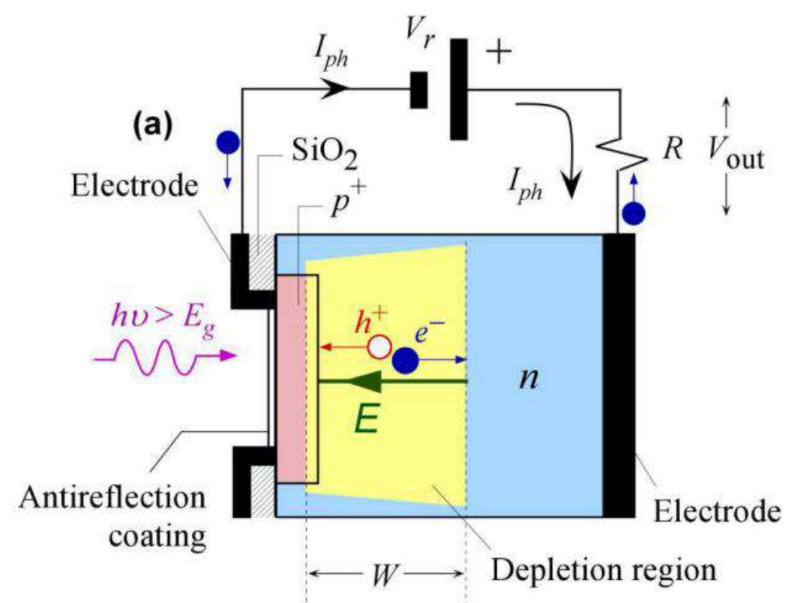
\includegraphics[scale=0.4]{images/3/inside_photodiode.png}
    \caption{Struttura di un fotodiodo.}
\end{figure}

Se un fotone entrante ha sufficiente energia, può creare un elettrone e un protone liberi nella regione di svuotamento.
A causa della polarizzazione inversa, l'elettrone partirà verso la zona \textit{n}, mentre il protone verso la zona \textit{p},
quindi troveremo l'elettrone in uscita dal catodo del diodo e in transito verso il polo positivo della batteria (pallina blu subito sopra il catodo),
mentre il protone uscirà dall'anodo e viaggerà verso il polo negativo della batteria, e può quindi essere rappresentato
da un elettrone che viaggia nel senso opposto (pallina blu entrante nell'anodo). Abbiamo quindi due elettroni che viaggiano dalla zona di svuotamento al catodo, per poi raggiungere il polo
positivo della batteria: per convenzione possiamo quindi porre una corrente $I_{ph}$ che gira nel senso opposto agli elettroni.

\subsection{Fotodiodi: approfondimento}
Cosa succede esattamente nel fotodiodo all'arrivo di un fotone dipende in realtà sia dal materiale di cui è fatto
il fotodiodo, che dall'energia del fotone. Minore è la frequenza del raggio del fotone (alta lunghezza d'onda, bassa energia), più
esso penetrerà in profondità. Poiché la luce si estende su un ampio spettro di lunghezze d'onda, capiterà
che alcune coppie di elettrone e protone verranno generate nella regione di svuotamento, altre invece nella zona \textit{p},
e altre nella zona \textit{n}. Però, non essendoci un campo elettrico al di fuori della regione di svuotamento, cariche generate al di fuori di essa
si muoveranno solo per diffusione, e quindi la cosa non funziona molto bene (non c'è la spinta del campo elettrico della zona di svuotamento, anzi, il campo si oppone al movimento
di una delle due cariche). È desiderabile che le coppie vengano generate nella regione di svuotamento.

\subsection{Modalità di operazione dei fotodiodi}

\renewcommand{\thefigure}{3.3}
\begin{figure}[!h]
  \centering
    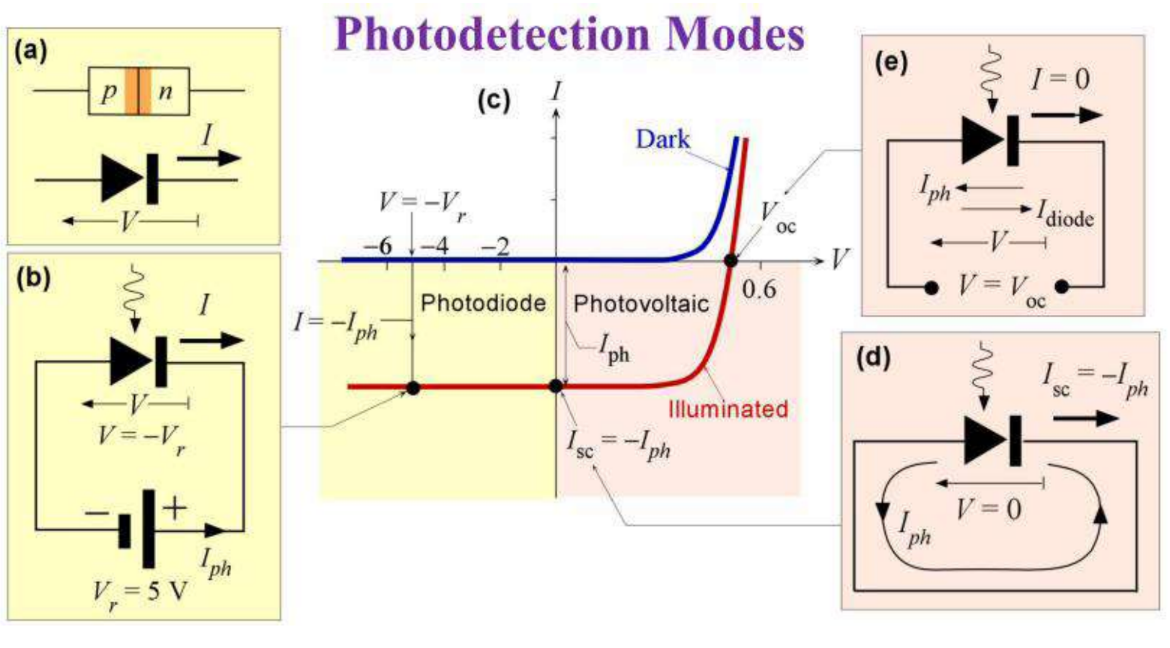
\includegraphics[scale=0.4]{images/3/photodiode_modes.png}
    \caption{Modalità di operazione di un fotodiodo.}
\end{figure}

Modalità ``fotodiodo'': è il quadrante in basso a sinistra del grafico (diodo inversamente polarizzato).
Se è buio (curva blu), (quasi) non c'è corrente che circola attraverso la giunzione, mentre se entrano dei fotoni,
allora c'è la corrente $I_{ph}$, che è opposta rispetto alla direzione convenzionale di scorrimento della corrente in un diodo
(cioè il ``verso della freccia''): quindi $I = -I_{ph}$.
$I_{ph}$ dipende linearmente dall'intensità della luce che colpisce il fotodiodo.
\par
L'aggiunta di un carico tra fotodiodo e batteria permette di misurare linearmente la quantità di luce in ingresso
nel fotodiodo. La retta di carico si costruisce prendendo il caso in cui attraverso il diodo (e quindi l'intero circuito) non
scorre alcuna corrente (quindi ai due capi della resistenza le tensioni sono uguali, $V = -V_{r}$), e poi il caso in cui
ai capi del diodo non vi sia alcuna caduta di potenziale ($V = 0$, quindi $I = (-V -V_r) / R_L = (0 - V_r)/R_L = -V_r / R_L$).

\renewcommand{\thefigure}{3.4}
\begin{figure}[!h]
  \centering
    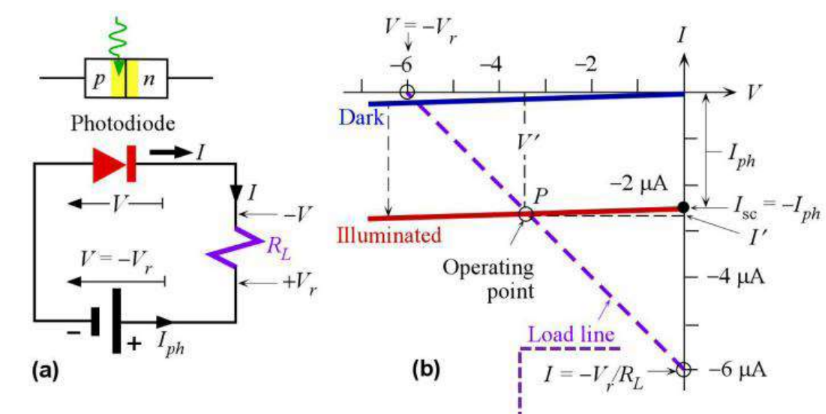
\includegraphics[scale=0.55]{images/3/load_line.png}
    \caption{Costruzione della retta di carico di un fotodiodo.}
\end{figure}


\subsection{Circuito equivalente per piccoli segnali}

\renewcommand{\thefigure}{3.5}
\begin{figure}[!h]
  \centering
    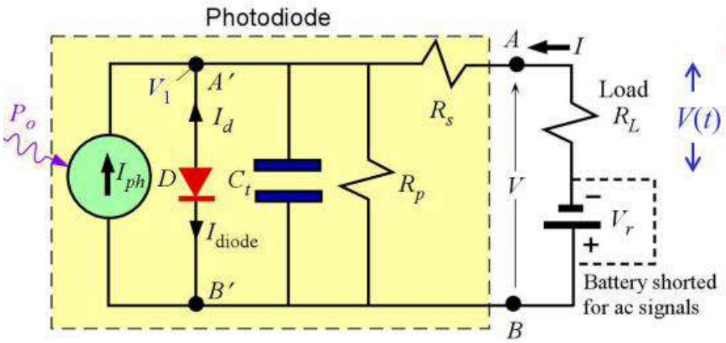
\includegraphics[scale=0.55]{images/3/equivalent.png}
    \caption{Circuito equivalente per piccoli segnali.}
\end{figure}

\begin{itemize}
    \item La sorgente di corrente emette la $I_{ph}$.
    \item Il diodo fa sì che questa corrente scorra soltanto nel senso desiderato.
    \item Il condensatore rappresenta l'effetto capacitivo della giunzione \textit{pn}.
    \item La resistenza di \textit{shunt} (in parallelo) fa parte del modello ideale della sorgente di corrente.
    Idealmente, è infinita, affinché tutta la corrente generata si diriga sul carico.
    \item La resistenza in serie è la resistenza interna del fotodiodo, idealmente è nulla.
    Nella realtà, il potenziale che ci cade sopra polarizza direttamente il diodo, riducendo la quantità
    di corrente che arriva sul carico (un poca verrà scaricata a terra tramite il diodo polarizzato).
\end{itemize}
Il condensatore e la resistenza in serie generano un effetto passa-basso, ma nelle applicazioni reali dei fotodiodi
la frequenza di taglio di questo filtro è sufficientemente alta da non creare problemi.

\subsection{Sensori di acquisizione}
Un pixel è composto dal fotodiodo, un condensatore che immagazzina le cariche generate, e della circuiteria
che permette l'indirizzamento dello specifico fotodiodo. Questa circuiteria consiste in un transistor MOSFET, che viene
attivato quando la \textit{address line} è alta, e riporta sulla linea di output dei dati (\textit{data line}) l'informazione presente nel condensatore. Questa struttura di un sensore
si chiama \textbf{indirizzamento attivo a matrice}.

\renewcommand{\thefigure}{3.6}
\begin{figure}[!h]
  \centering
    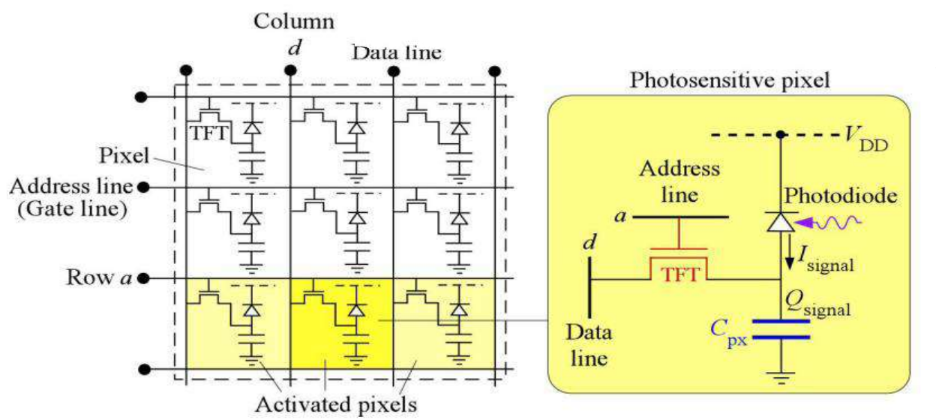
\includegraphics[scale=0.5]{images/3/ama.png}
    \caption{Matrice di 9 pixel con indirizzamento attivo.}
\end{figure}

Come acquisire i colori? Ci sono due modi: il primo consiste nello scomporre la luce nelle tre componenti
fondamentali attraverso un prisma, e dirigere i tre fasci verso tre sensori dedicati. Poi in qualche modo queste informazioni
verranno combinate insieme. Costoso e complicato.
\newline
Il secondo metodo sfrutta il filtro di Bayer. Sopra la griglia dei pixel si mette una griglia di plastica che filtra la luce e permette solo a certi colori di
raggiungere il pixel sottostante. Servono più pixel di base per costruire un vero pixel a colori (rapporto 1:4), l'informazione di un gruppo di 4 pixel dovrà essere interpolata
per produrre il valore finale di un ``macropixel'' a colori.

\renewcommand{\thefigure}{3.7}
\begin{figure}[!h]
  \centering
    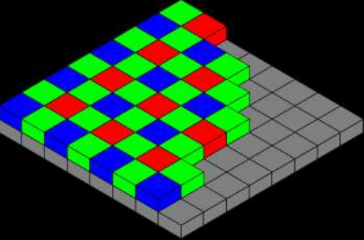
\includegraphics[scale=0.5]{images/3/bayer.png}
    \caption{Filtro di Bayer.}
\end{figure}

Il filtro \textit{X-Trans} è una versione migliorata del filtro di Bayer. Utilizza una disposizione meno regolare delle celle rosse, verdi e blu. Aiuta a ridurre
l'effetto Moiré e i problemi di falso colore senza l'uso di un filtro passa-basso ottico, ma richiede più computazione per combinare l'informazione di ciascun pixel.

\renewcommand{\thefigure}{3.8}
\begin{figure}[!h]
  \centering
    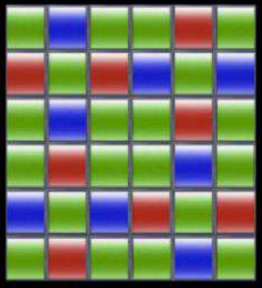
\includegraphics[scale=0.5]{images/3/xtrans.png}
    \caption{Filtro X-Trans.}
\end{figure}

\subsection{Sensori CCD}
Sono dei registri a scorrimento che funzionano spostando cariche.
Ogni cella ha tre elettrodi, che vengono usati per creare dei ``pozzi'' e delle barriere di potenziale,
che confinano gli elettroni in una determinata zona. Creando degli array di singole celle e collegando tra loro tutti
gli elettrodi di sinistra, centrali e di destra, facendoli comandare da dei segnali di clock sfasati di 120° tra loro,
ottengo un registro a scorrimento che trasporta le cariche.

\renewcommand{\thefigure}{3.9}
\begin{figure}[!h]
  \centering
    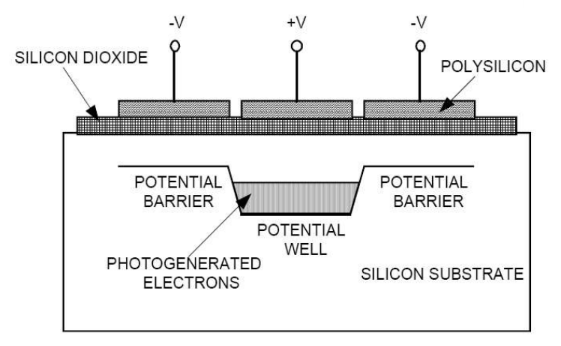
\includegraphics[scale=0.5]{images/3/ccd_cell.png}
    \caption{Una cella di un sensore CCD: gli elettroni si accumulano di fronte all'elettrodo con potenziale positivo.}
\end{figure}

\renewcommand{\thefigure}{3.10}
\begin{figure}[!h]
  \centering
    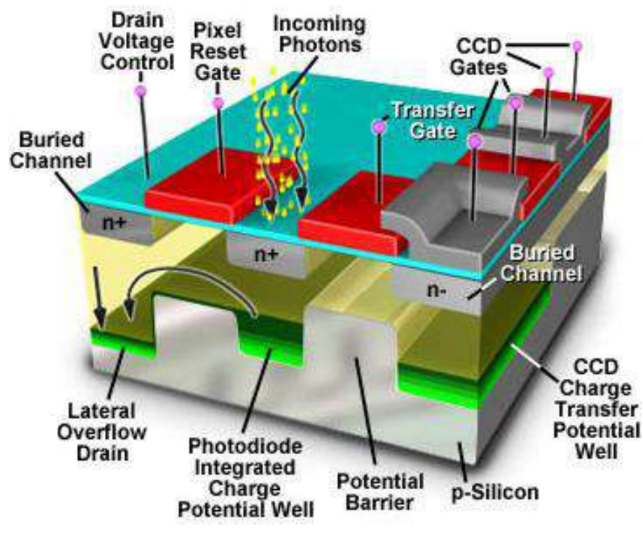
\includegraphics[scale=0.5]{images/3/photodiode_ccd.png}
    \caption{Fotodiodo all'interno di un sensore CCD.}
\end{figure}

Nell'immagine qui sopra, sul piano frontale si vede il fotodiodo (l'elemento su cui incidono i fotoni). Una volta terminata l'acquisizione,
tramite il \textit{transfer gate} gli elettroni vengono trasferiti nella cella CCD (``lago'' verde a destra), che poi comincia a trasportarli via verso il retro del disegno, tramite i \textit{CCD gates}.
Quando troppa luce incide sul fotodiodo, si generano così tante cariche che alcune potrebbero trasbordare in un fotodiodo adiacente, rovinando la qualità dell'acquisizione
(effetto \textit{blooming}).
Per questo motivo esiste il \textit{lateral overflow drain}, dove eventuali cariche in eccesso possono depositarsi ed esser gettate via.

\renewcommand{\thefigure}{3.11}
\begin{figure}[!h]
  \centering
    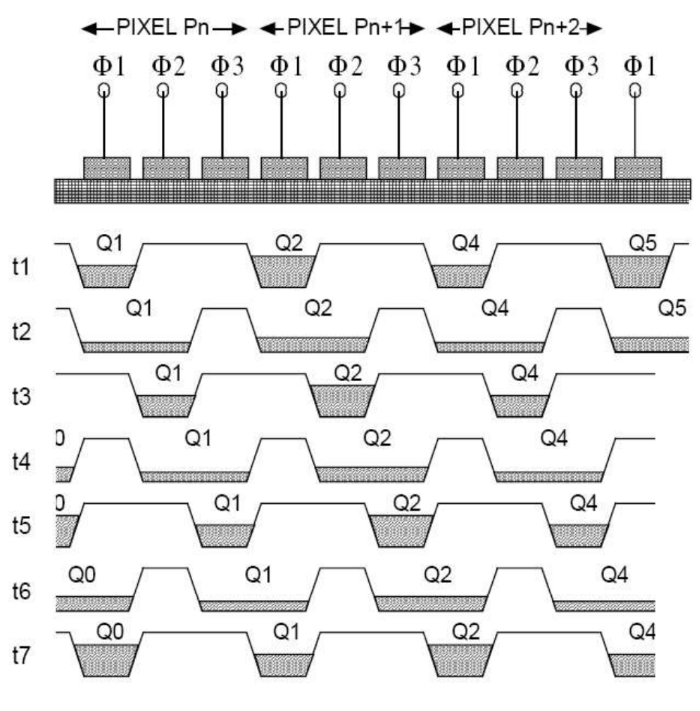
\includegraphics[scale=0.5]{images/3/shifting.png}
    \caption{Scorrimento delle celle.}
\end{figure}

Qui si vede come, a diversi istanti di tempo, vengono regolati i potenziali degli elettrodi di ciascun pixel in modo che le cariche generate da ciascun fotodiodo si avvicinino
all'uscita del circuito (che sarà verso destra). Bisogna tenere sempre in attività un sensore CCD, usando quindi dei clock abbastanza veloci, altrimenti si genera del rumore termico
che produce nuovi elettroni.

\renewcommand{\thefigure}{3.12}
\begin{figure}[!h]
  \centering
    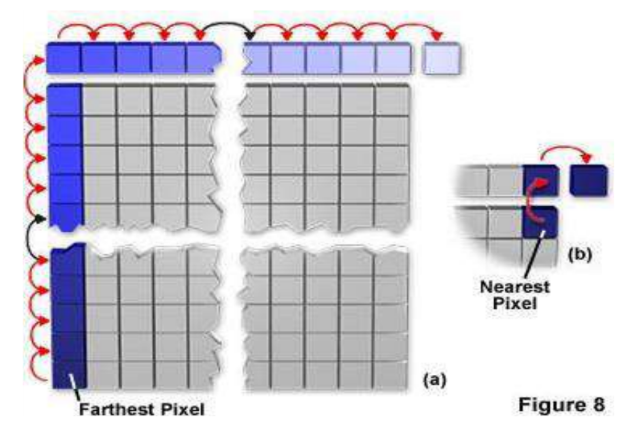
\includegraphics[scale=0.5]{images/3/outputting.png}
    \caption{Lettura dell'immagine in un sensore CCD.}
\end{figure}

Per leggere i dati da un sensore CCD, si trasla la matrice di dati provenienti dai pixel verso l'alto (utilizzando un registro che sta sul sensore, che sposta ogni pixel di 1 posizione verso l'alto),
cosicché la riga grigia che si trova in cima venga spostata nel registro orizzontale (riga blu). A quel punto, una serie di scorrimenti manda in
output i pixel della riga orizzontale uno alla volta, dal primo a destra fino all'ultimo a sinistra. In output, c'è un amplificatore controllato in corrente (CCVS) che amplifica i segnali.
\par
A che velocità devono girare i due registri, se ad esempio voglio catturare 30 fotogrammi di dimensione 1000x1000 pixel al secondo?
Il registro orizzontale deve lavorare 1000 volte più velocemente dei registri sul sensore, che si occupano di traslare ogni riga della matrice
verso l'alto. Questo perché se la matrice viene traslata 1 volta al secondo, il registro orizzontale ha 1 secondo di tempo per mandare
in output tutti i 1000 pixel che contiene, prima che arrivino i successivi dati della riga sottostante.
Il registro orizzontale deve fare $10^6$ scatti in $1/30$ di secondo, quindi il suo clock dovrà essere di 30 MHz. I registri sul sensore invece dovranno girare a 30 kHz.
\par
Le due problematiche principali dei sensori CCD sono:
\begin{itemize}
    \item il rumore termico, che produce elettroni che vanno a sporcare il dato raccolto dal fotodiodo. La
    \textit{dark current} altro non è che rumore termico in condizioni di buio totale.
    Il rumore termico cresce esponenzialmente all'aumentare della temperatura;
    \item l'efficienza di trasferimento: l'informazione raccolta dal pixel più lontano dall'output deve sopravvivere a molti più spostamenti;
\end{itemize}

\subsubsection{Architetture CCD}
Apertura: quantità di spazio, in una cella fotosensibile, che può essere dedicata all'acquisizione di luce.
\begin{enumerate}
    \item \textit{Full frame}: non hanno un'area di archiviazione. Dopo aver catturato l'immagine, bisogna chiudere l'otturatore, e mandare in output ciò che si ha catturato. Poi si può riaprire l'otturatore
    e catturare una nuova immagine. Il ciclo di funzionamento è lento, però l'apertura è del 100\%.
    \item \textit{Frame transfer}: c'è una matrice di archiviazione sotto la matrice di pixel. Dopo aver catturato un'immagine, si spostano le cariche nella matrice di archiviazione, e mentre queste vengono
    mandate in output dai registri a scorrimento, si può già catturare una nuova immagine. Realizzazione circuitale più semplice. L'apertura è del 50\%, confrontata con quella di un sensore \textit{full frame} 
    delle stesse dimensioni fisiche. Otturatore non necessario se il tempo richiesto per spostare le cariche nella matrice di archiviazione è sufficientemente piccolo. Altrimenti serve, perché i pixel
    continuerebbero a integrare tanta luce mentre avviene questo spostamento, e se la scena presentasse un oggetto molto chiaro e luminoso, l'immagine potrebbe
    contenere una sgradevole striscia chiara.
    \item \textit{Interline transfer}: ogni colonna di pixel ha accanto a sé un registro verticale (non si vedeva nell'immagine precedente che ne raccoglie i dati e li manda verso l'alto o il basso, dove c'è il
    registro orizzontale di output. Lo spostamento delle cariche da ogni cella fotosensibile alla sua cella di archiviazione è quindi molto veloce, l'otturatore non serve. Apertura del 50\% circa.
\end{enumerate}

\renewcommand{\thefigure}{3.13}
\begin{figure}[!h]
  \centering
    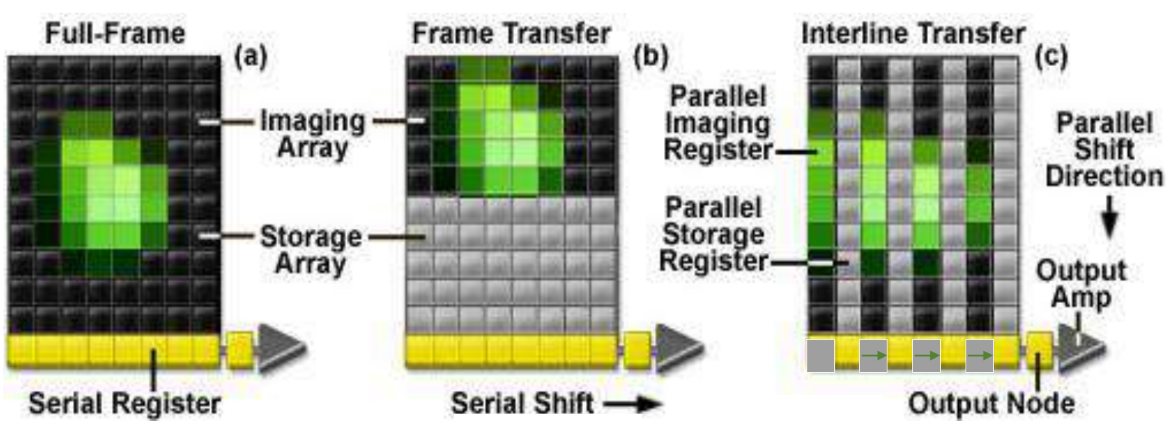
\includegraphics[scale=0.4]{images/3/archs.png}
    \caption{Architetture dei sensori CCD.}
\end{figure}

Nelle ultime due architetture i clock dei registri CCD fungono da otturatore elettronico, cioè regolano il tempo di acquisizione
del fotodiodo.
\par
Il sensore CCD e la scheda su cui stanno tutte le altre componenti della filiera di processamento di un'immagine
sono due pezzi di hardware separati, questo perché un sensore CCD richiede una struttura fisica della scheda che non è compatibile
con la tecnologia CMOS, usata per produrre tutte le altre componenti. Anche i macchinari industriali da usare sono diversi, e tutto questo fa aumentare i costi di produzione. Meglio cercare altre soluzioni, compatibili con la tecnologia CMOS, come i...

\subsection{Sensori CMOS}

\renewcommand{\thefigure}{3.14}
\begin{figure}[!h]
  \centering
    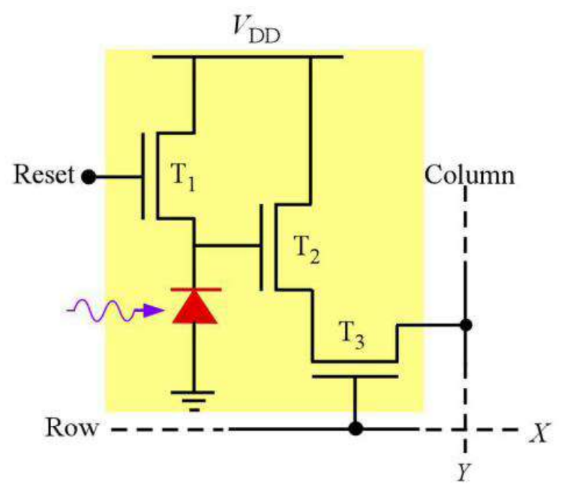
\includegraphics[scale=0.4]{images/3/cmos_cell.png}
    \caption{Cella di un sensore CMOS.}
\end{figure}

Il fotodiodo è sempre presente. T1 è semplicemente un transistor di reset: all'inizio del processo di acquisizione, lo si attiva (il catodo del diodo viene portato
al potenziale $V_{DD}$) e poi lo si disattiva (il catodo del diodo rimane a $V_{DD}$). Ora la luce comincia a incidere sul fotodiodo, e quindi si genera una corrente che scorre
nel verso opposto alla ``freccia'' del fotodiodo. Questa corrente contribuisce a diminuire la differenza di potenziale tra i capi del fotodiodo (non sarà più $V_{DD}$,
ma un po' di meno). Tanta più luce colpisce il fotodiodo, tanto più intensa sarà questa corrente, tanto più grande sarà la diminuzione della differenza di potenziale.
T2 è un transistor il cui gate è controllato proprio da questa differenza di potenziale, e ipotizzando che questa tensione sia tale da mandarlo in saturazione, esso
opererà come un amplificatore. Ecco che quindi T2, sul suo source, fornirà a T3 il segnale
che vede sul proprio gate, ma amplificato! E T3, quando il segnale X si alza per leggere la riga su cui giace, riporta sulla colonna Y il dato.
Ricapitolando, T1 e T3 vengono usati come interruttori CMOS (quindi in regime lineare), mentre T2 viene usato come amplificatore, in regime di saturazione.

\par
Problema: l'apertura è bassa! I transistor occupano molto spazio, in un pixel. La luce che li colpisce viene persa.
Possibile soluzione: sopra ogni sensore può esserci una matrice di microlenti, per focalizzare la luce esattamente su ciascun fotodiodo.
Questo produce una sorta di guadagno artificiale.
Gli svantaggi sono che bisogna produrre questa matrice (e costa), e che queste microlenti assorbono un po' di luce. Nonstante questi svantaggi, è una pratica spesso usata.
\par
Ogni pixel, dunque, ha il suo amplificatore che converte le cariche in una tensione, ed è chiaro che questi
transistor non saranno mai uguali ta loro al 100\%: diversi pixel amplificheranno i segnali in modo leggermente diverso,
e questo genera un tipo di rumore denominato ``rumore a pattern fisso'' (\textit{fixed pattern noise}).
È un rumore che è noto (fino a un certo punto), perché dipende dalle caratteristiche fisiche dei transistor (ma anche dalla temperatura, ad esempio).
Possiamo stimarlo acquisendo un'immagine uniforme e osservando le disomogeneità (facile a dirsi, ma trovare un modo per acquisire un'immagine uniformemente bianca
è piuttosto difficile).

\subsection{Datasheet}
\subsubsection{Si Photodiodes (Hamamatsu)}
Si nota come molti sensori in commercio siano sensibili alla luce infrarossa. Questo è un bene, perché permette di
costruire una fotocamera a infrarossi piuttosto facilmente, ma è anche un male, perché quando l'energia infrarossa (energia termica) non mi interessa, posso sì cercare di filtrarla, ma non
riuscirò mai a eliminarla del tutto, e quindi impatterà un minimo sull'acquisizione.

\subsubsection{Selection guide (Hamamatsu)}
I sensori CCD sono più costosi e usati principalmente in ambito scientifico/industriale.
\par
Sensore CCD illuminato frontalmente: è quello ``classico'', l'apertura è buona, ma non del 100\%: anche nei sensori CCD c'è
dell'elettronica (gli elettrodi che ne regolano il funzionamento) che occupa spazio. Se si vuole massimizzare l'apertura, bisogna usare i sensori CCD \textit{back-thinned},
che catturano la luce da dietro. Il substrato di silicio del chip deve essere molto molto sottile, cosicché la luce possa attraversarlo e raggiungere
la regione di svuotamento. Per acquisire un'immagine in condizioni di scarsa luce, bisogna raffreddare il sensore, così il rumore termico viene ridotto.
\par
I \textit{distance image sensor} sono sensori che riescono a produrre un'immagine tridimesionale dell'oggetto. Quelli di
Hamamatsu usano la tecnica basata sul tempo di volo (\textit{time of flight}, TOF): un dispositivo illuminante genera un impulso
luminoso, poi il sensore ne cattura il riflesso e ricostruisce la profondità sulla base del ritardo
con cui il riflesso è tornato indietro.
\par
I sensori per le immagini a raggi X non sono dei semplici fotodiodi sensibili alle lunghezze d'onda dei raggi X,
perché i raggi X distruggerebbero l'elettronica di un normale sensore di acquisizione. Quello che fanno
è convertire un raggio X in un fotone (particella a minore energia) usando uno scintillatore, e poi acquisicono quel fotone.

\subsubsection{Sensore CCD KAI-50140 (On Semiconductors)}
\begin{itemize}
    \item Capienza (per le cariche): quante cariche possono essere immagazinate per ogni fotodiodo, prima
    che si inizi ad avere effetto \textit{blooming}.
    \item Sensibilità dell'output: dipende dalle caratteristiche dell'amplificatore che converte le cariche in tensoni.
    \item Efficienza quantica: dice quanti fotoni vengono convertiti in informazione utile.
    I valori variano tra le tre diverse bande, il che non è un bene, ovviamente: sarebbe bello avere una
    cattura omogenea delle diverse bande di colore.
    \item \textit{Read noise}: il rumore complessivo che si ha nel sensore. Combinato con la capienza per le cariche, ci dà
    l'intervallo dinamico del sensore.
    \item Intervallo dinamico: è l'ampiezza dell'intervallo di illuminanza che può essere convertito dal sensore.
    Si ottiene dividendo la capienza per il \textit{read noise}. Questo calcolo ci dà il numero di livelli distinguibili
    di carica che possono essere immagazinati nel pozzo di elettroni: interpretando il \textit{read noise} come
    l'ampiezza ``quantizzata'' di un livello (scostamenti minori del \textit{read noise} non possono essere rilevati),
    la formula rappresenta semplicemente il classico modo di calcolare il numero di livelli in un intervallo:
    \[\frac{max-min}{stepsize}\]
    Dove $max$ è la capienza, $min$ è 0, e $stepsize$ è il \textit{read noise}.
    La conversione in decibel avviene con la formula $X_{db} = 20 \cdot  \log_{10}(X)$
\end{itemize}
Pixel scuri di riferimento: sono una porzione dei pixel del sensore che è schermata, in modo che la luce non possa raggiungerli.
Si usano per stimare qual è il segnale prodotto sui pixel normali in condizioni di buio totale.

\subsubsection{Sensori CMOS NOIP1SN0xyKA (On Semiconductors)}
Regione d'interesse programmabile: siccome sono sensori molto grandi, bisogna trasferire un'immagine molto pesante
al resto del circuito in breve tempo. Se mi interessa solo una porzione dell'immagine totale,
posso programmare quest'informazione nel sensore, e lui eseguirà il trasferimento rapido di solo quella porzione.

\subsubsection{Sensore CCD a moltiplicazione di elettroni (Andor)}
Per applicazioni scientifiche, è in grado di catturare singoli fotoni.
Due possibili approcci:
\begin{enumerate}
    \item intensificatore di immagine: c'è un dispositivo che cattura un fotone e ne genera tanti (moltiplicatore di fotoni);
    \item moltiplicatore di cariche: converto il singolo fotone in una coppia di elettrone e protone, poi moltiplico questi ultimi. Più economico, ma funziona peggio.
\end{enumerate}
Come realizzare un moltiplicatore di cariche? Uso dei speciali CCD che permettono di creare dei pozzi di potenziale
molto profondi. Un singolo elettrone, cadendoci, acquisice così tanta energia dovuta al potente campo elettrico, da generare
nuove cariche (prenderlo per vero senza farsi troppe domande).
C'è un problema dovuto alle temperature! Devono essere molto basse, altrimenti molti degli elettroni che il sensore moltiplica saranno dovuti al rumore termico.
C'è anche un problema dovuto al fatto che questi sensori moltiplicano la luce in modo probabilistico: dato un singolo elettrone che cade
nel pozzo, non ho certezze su quanti altri elettroni produrrà. È probabile che un elettrone cadente ne produca meno di
quanti ne producano due elettroni cadenti, ma non posso controllare il processo.

\subsubsection{Sensori a punti quantici}
Un punto quantico è un pezzo di semiconduttore così piccolo che al suo interno si generano effetti quantistici.
In particolare, avviene il \textit{quantum confinement}. L'energia del fotone che viene ricevuto può essere selezionata
con precisione. Posso scegliere di ricevere una specifica tonalità semplicemente costruendo un punto quantico
di una certa dimensione e di un certo materiale. Al contrario, si possono usare questi punti quantici per generare luce ad una frequenza molto precisa: costruisco così gli schermi a punti quantici.

\subsection{Sensori ad ampio intervallo dinamico (HDR)}
60 dB di intervallo dinamico (valore tipico per un normale sensore) non sono molti. Una scena potrebbe avere un intervallo dinamico molto più ampio,
cioè le zone in ombra potrebbero essere molto scure e le zone illuminate molto chiare.
\par
Un possibile modo di risolvere questo problema è quello di rendere la risposta del fotodiodo nonlineare, tramite della circuiteria apposita. Però così
si perde la comoda relazione lineare tra luce entrante nel fotodiodo e cariche generate... Meglio cercare soluzioni alternative.

\subsubsection{HDR con sensori multipli}
Un altro approccio è quello di avere due sensori per ogni pixel. Uno è un sensore ad alta sensibilità (per le zone scure),
l'altro è a bassa sensibilità (per le zone chiare). Ora vediamo un esempio in cui ci sono tre sensori per pixel (bassa, media e alta sensibilità).

\renewcommand{\thefigure}{3.15}
\begin{figure}[!h]
  \centering
    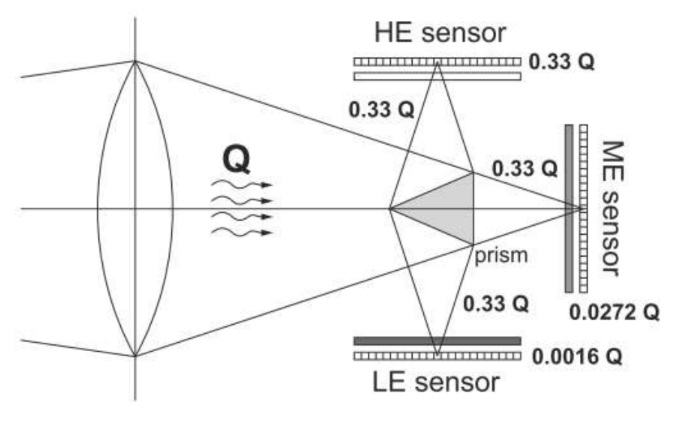
\includegraphics[scale=0.4]{images/3/trisensor_naive.png}
    \caption{Pixel HDR con tre sensori.}
\end{figure}

Questo sistema è complesso dal punto di vista meccanico. Abbiamo un prisma che scompone la luce e la divide in tre fasci,
ciascuno direzionato ad uno dei sensori. L'energia è divisa in  tre parti uguali.
I tre sensori sono in realtà identici, ciò che ne cambia la sensibilità è la presenza di un filtro più o meno assorbente
davanti. È chiaramente una soluzione che sfrutta la luce in modo poco efficiente.
\par
Meglio usare dei \textit{beam splitter}, dispositivi di plastica che, in base all'angolo di incidenza della luce, ne riflettono una parte e si lasciano attraversare dal resto della luce.

\renewcommand{\thefigure}{3.16}
\begin{figure}[!h]
  \centering
    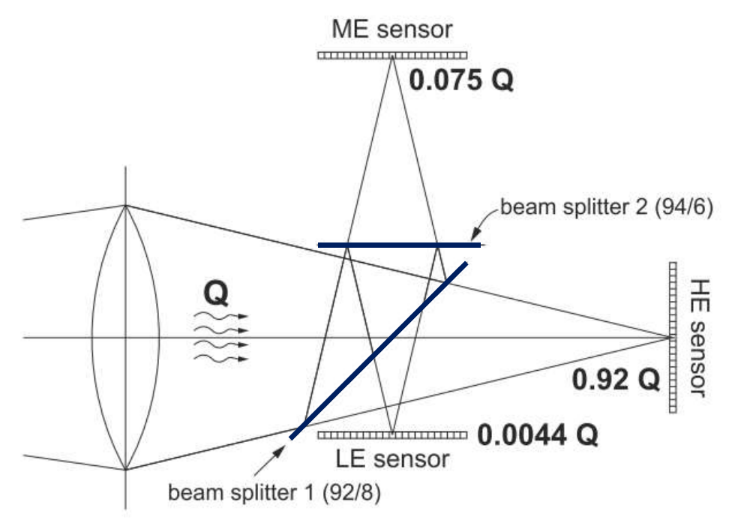
\includegraphics[scale=0.4]{images/3/trisensor_beam.png}
    \caption{Pixel HDR con tre sensori, versione migliorata.}
\end{figure}

Dopo l'acquisizione, bisogna unire i dati provenienti dai tre sensori in qualche modo; prima, però, bisogna aver calibrato tra di loro i sensori, in modo da sapere come interpretare
le informazioni che ci forniscono. Vediamo ora come.

\subsubsection{La funzione di trasferimento della fotocamera}
Dobbiamo conoscere questa funzione per poter dare significato ai dati che i sensori ci forniscono.
Per ogni pixel, si definisce l'esposizione come $X = E \cdot \Delta t$, dove $E$ è l'irradianza, mentre $\Delta t$
è il tempo di esposizione. La funzione di trasferimento è quindi definita come $Z = f(X)$. Questa
funzione è nonlineare: per alti valori dell'argomento, satura. Questo effetto è introdotto volontariamente dai produttori,
per ragioni storiche: si voleva che i sensori digitali si comportassero come quelli analogici, basati sulla pellicola.

\renewcommand{\thefigure}{3.17}
\begin{figure}[!h]
  \centering
    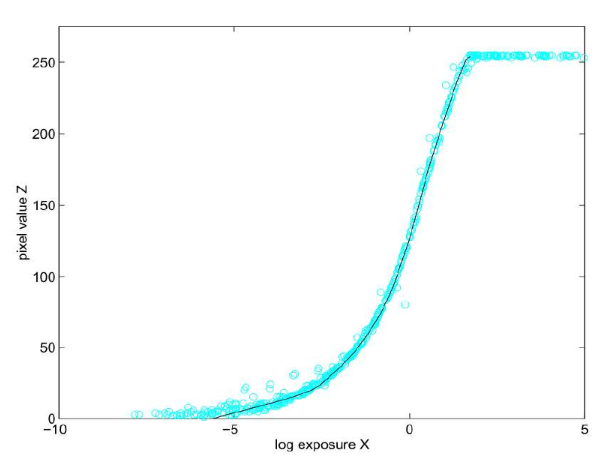
\includegraphics[scale=0.6]{images/3/sensor_transfer_function.png}
    \caption{Funzione di trasferimento di una fotocamera. Si nota la saturazione per alti valori di X.}
\end{figure}

Ora, scattiamo 5 foto di una stessa scena con diversi tempi di esposizione, e analizziamo i livelli di grigio
di 3 pixel in ciascuna immagine (sempre gli stessi 3 pixel, nelle stesse posizioni). Noi conosciamo l'intensità luminosa di quei 3 punti,
e se anche non la conosciamo esattamente, conosciamo il tempo di esposizione usato. Possiamo quindi iniziare a ricostruire il grafico della funzione $f^{-1}()$.

\renewcommand{\thefigure}{3.18}
\begin{figure}[!h]
  \centering
    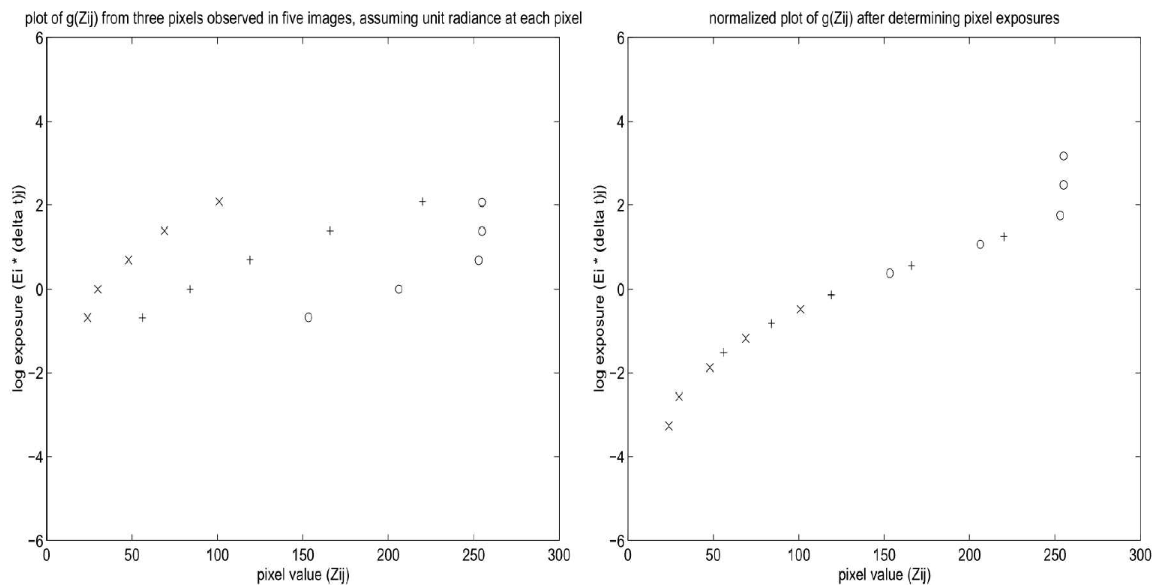
\includegraphics[scale=0.4]{images/3/inverse.png}
    \caption{Ricostruzione di $f^{-1}()$.}
\end{figure}

Posizioniamo i punti che rappresentano uno stesso pixel a dei valori esatti sull'asse delle ascisse (conosciamo per forza i livelli di grigio di tutti i pixel),
e ad un'altezza arbitraria sull'asse delle ordinate (la differenza di altezza tra le 5 catture di ciascun pixel non è arbitraria, è nota poiché conosciamo $\Delta t$, è arbitraria
la quota a cui gli interi gruppi di $\times$/+/$\circ$ sono posti).
\newline
Poiché appunto le quote precise sono ancora ignote, andiamo a traslare verso l'alto o il basso ciascun gruppo, in modo che i vari simboli si allineino a formare il grafico della funzione
inversa della funzione di trasferimento vista prima. L'idea è quella di avere tre sensori che complessivamente si comportano come uno solo, ma ognuno dei tre si occupa solo
di una parte del lavoro (uno lavora a basse, uno a medie, uno ad alte esposizioni).
\newline
Terminato questo lavoro, l'ordinata dell'intera curva è ancora arbitraria, ma va bene così, non è un problema: a noi interessa calibrare i sensori tra di loro, non in senso assoluto.

\subsubsection{HDR con sensori multipli - continuazione}
Ora che conosciamo l'offset relativo da applicare in verticale ai punti catturati dai vari sensori
per diversi valori di esposizione, abbiamo un modo di combinare le informazioni provenienti dai tre sensori per ottenere un'unica immagine HDR finale. Come farlo, in pratica?
\par
Per semplicità poniamo che i sensori abbiano come output solo 16
valori di grigio, invece di 256.
La combinazione dei tre sensori con pesi triangolari (linea tratteggiata blu nell'immagine qui sotto) è un modo semplice ma non ottimale per farlo. Vediamo perché.
\par
Il sensore ad alta esposizione satura molto presto, quindi i suoi 16 livelli di grigio sono compattati in un ``dominio''
(cioè un intervallo all'interno del quale il sensore dà informazione utile) molto stretto
(dall'illuminanza nulla fino a quella di saturazione, appunto). I suoi 16 valori rappresentano quindi digitalmente
un'informazione analogica (questa illuminanza) con un errore di quantizzazione abbastanza piccolo.
Il sensore a bassa esposizione, invece, lavora in un dominio molto più ampio, quindi i suoi 16 valori
devono coprire un intervallo largo: l'errore di quantizzazione è più alto. Di conseguenza, per minimizzare gli
errori di quantizzazione, l'approccio migliore è quello di usare sempre i dati provenienti dal sensore
a esposizione più alta tra quelli disponibili, con solo delle zone di transizione tra uno e l'altro (pesi trapezoidali, linee continue nere nell'immagine).

\renewcommand{\thefigure}{3.19}
\begin{figure}[!h]
  \centering
    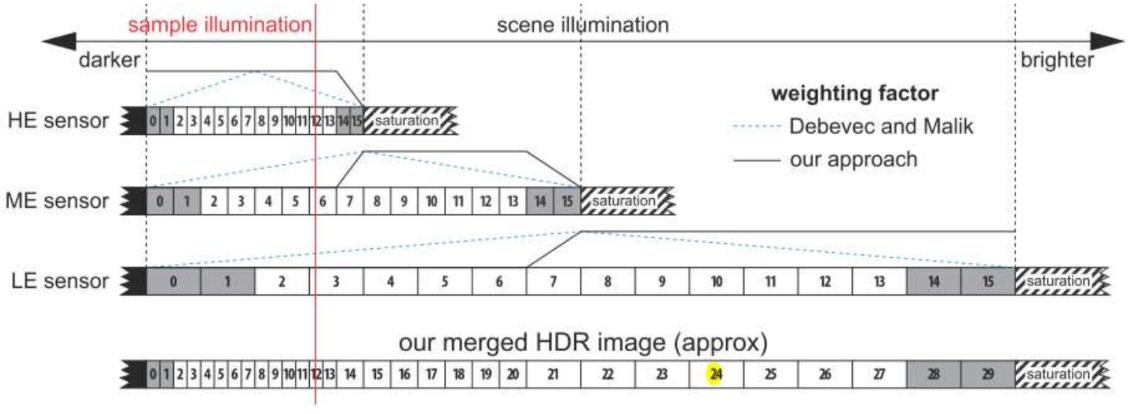
\includegraphics[scale=0.4]{images/3/combination.png}
    \caption{Combinazione delle tre immagini.}
\end{figure}

\subsubsection{HDR con cattura sequenziale}
Il sistema a tre sensori è molto complesso, costoso, e richiede parecchio spazio fisico per essere realizzato.
In molte applicazioni, serve una soluzione più semplice ed economica. Si può ad esempio usare un unico sensore,
e catturare tre immagini, con diversa esposizione, in sequenza. Qui il problema è che spesso la fotocamera e la scena
non sono immobili!
\subsubsection{Sensore AR0331 (On Semiconductors)}
Può operare in regime lineare (LDR, \textit{low dynamic range}) oppure pseudo-logaritmico (modalità HDR, appunto). In modalità LDR, utilizza un \textit{rolling shutter}:
la prima riga viene attivata, integra luce, porta i valori in output. Dopodiché, viene attivata la seconda riga, dopo la terza, ecc.
Quindi, le varie righe vengono acquisite in tempi leggermente diversi. I valori digitali hanno una risoluzione di 12 bit per pixel.
In modalità HDR, la risoluzione sale a 16 bit per pixel, con possibilità di compressione a 12 bit (per compatibilità).
\par
Questo sensore utilizza la cattura sequenziale: acquisisce due immagini con diverse esposizioni. Il
\textit{rolling shutter} è in realtà doppio: quando il primo è sceso un poco, parte il secondo,
che inzia a catturare la seconda immagine con esposizione diversa. Due righe di sensori sono quindi attive
in ogni momento (a parte i brevi transitori iniziale e finale).

\subsubsection{\textit{Deghosting}}
Un algoritmo di \textit{deghosting} è necessario per rimediare agli effetti dovuti al movimento, nei casi di cattura sequenziale.
Bisogna anche riadattare la luminosità: parti del soggetto forniscono più o meno luce in una stessa scena (non chiaro), e poi bisogna combinare il tutto per ottenere
l'immagine HDR.

\renewcommand{\thefigure}{3.20}
\begin{figure}[!h]
  \centering
    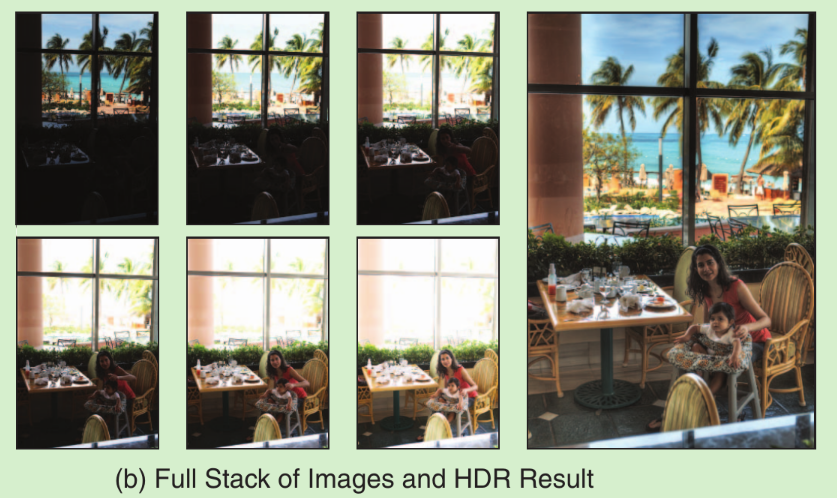
\includegraphics[scale=0.5]{images/3/hdr_example.png}
    \caption{Sei immagini con diverse esposizioni danno un'immagine HDR finale.}
\end{figure}

L'immagine finale non è fotorealistica! Il paesaggio fuori dalla finestra ha in realtà un'intensità luminosa molto più alta del resto della scena (come si nota nei sei scatti parziali),
ma nell'immagine HDR è riportato a dei valori di intensità più vicini ai valori medi, perché né i dispositivi di cattura né gli schermi
sarebbero altrimenti in grado di visualizzarlo in modo appropriato.
\par
L'idea di base di un algoritmo di deghosting è di rifiutare le parti delle varie immagini che non sono allineate tra loro,
a meno che non siano allineabili tramite transformazioni rigide. In questo caso significa che la scena
era statica ma la fotocamera si è mossa: rimediare è tutto sommato facile. Altrimenti serve un sistema
più complesso che modifichi la struttura geometrica degli oggetti (dettagli non visti).

\newpage

\subsection{Processo di acquisizione di un'immagine}

\renewcommand{\thefigure}{3.21}
\begin{figure}[!h]
  \centering
    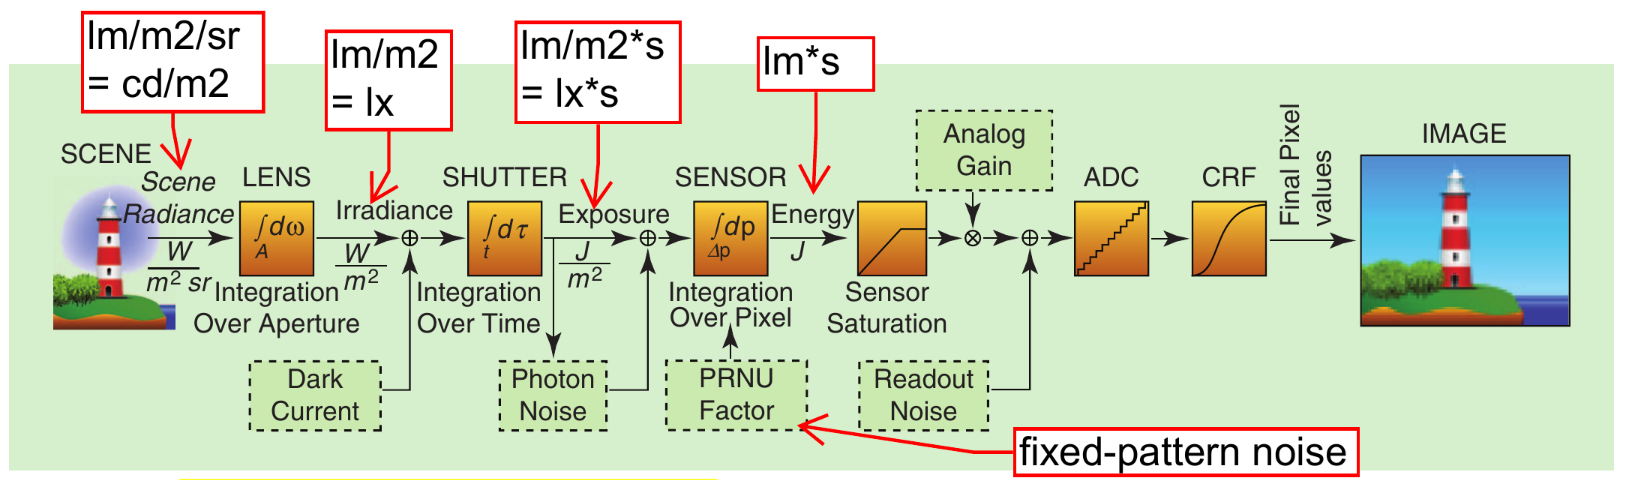
\includegraphics[scale=0.25]{images/3/pipeline.png}
    \caption{Processo di acquisizione di un'immagine.}
\end{figure}

\begin{enumerate}
    \item La scena ha una sua radianza, che colpisce la lente.
    \item La lente integra la radianza sulla sua apertura (l'apertura è una proprietà della lente). Intuitivamente, un singolo pixel somma tutta la luce che gli arriva da ogni angolo.
    Si ottiene un'irradianza: avendo sommato i contributi provenienti da ogni angolo solido (cioè direzione), l'unità di misura perde gli steradianti al denominatore.
    \item L'otturatore integra nel tempo l'irradianza. Sommando i contributi di potenza per unità di superficie si ottiene un'energia (per unità di superficie): otteniamo l'esposizione.
    \item Ogni pixel integra l'esposizione sulla sua superficie, il che rimuove l'unità di misura della superficie dal denominatore. Otteniamo un'energia.
    \item Questa energia viene amplificata e convertita in valori digitali.
    \item Come ultimo passaggio, se la fotocamera non prevede la cattura grezza dell'immagine (formato RAW), si passa per una funzione di trasferimento progettata dal produttore della fotocamera,
    per dare il risultato migliore possibile che si possa ottenere con la fotocamera usata.
\end{enumerate}

\par
In questo processo di acquisizione, ci sono diverse fonti di rumore:
\begin{itemize}
    \item quello termico, che dipende dal tempo di esposizione (per questo entra in gioco prima dell'otturatore);
    \item quello dovuto al tasso di arrivo dei fotoni sul sensore (è legato alla natura quantistica della luce). È rilevante soprattutto a basse esposizioni;
    \item il rumore a pattern fisso (solo se il sensore è CMOS);
    \item il rumore di lettura (cariche generate termicamente al momento della lettura di ogni pixel).
\end{itemize}

Queste fonti di rumore limitano la possibilità e la precisione del rilevamento di valori bassi di illuminazione della scena, mentre la capacità massima di un fotodiodo limita la quantità
di cariche generabili in condizioni di alta illuminazione. Di conseguenza, l'intervallo dinamico di un normale sensore è piuttosto basso.

\subsection{Fotocamere plenottiche}
Anche note come ``fotocamere a campo di luce'' (\textit{light-field camera}). L'idea è di tenere conto della direzione dei raggi luminosi che incidono
sul sensore. Si perde in risoluzione: un pixel non riceve più la luce che gli arriva da tutte le direzioni,
ma solo da un certo insieme ristretto di direzioni: servono più pixel per ogni posizione dell'immagine.
\par
L'uso di fotocamere plenottiche ci permette di stimare la distanza tra gli oggetti e la fotocamera, e di modificare la messa a fuoco dopo lo scatto.

\subsubsection{Fotografia stenopeica}
Tecniche che sfruttano le fotocamere stenopeiche/camere oscure (\textit{pinhole camera}).

\renewcommand{\thefigure}{3.22}
\begin{figure}[!h]
  \centering
    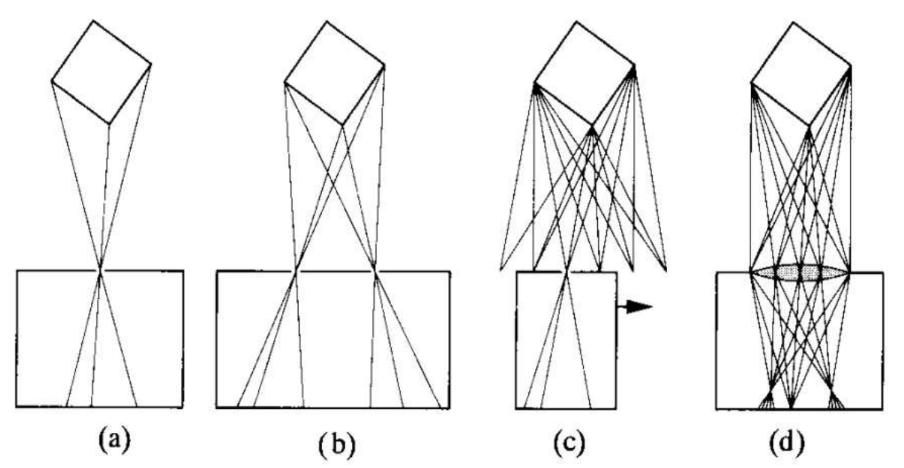
\includegraphics[scale=0.4]{images/3/pinholes.png}
    \caption{Quattro tipi di camera oscura.}
\end{figure}

\begin{enumerate}
    \item Camera oscura con 1 foro: offre un'immagine dell'oggetto.
    \item Camera oscura con 2 fori: offre due immagini dell'oggetto da due diversi punti di vista (fotografia stereoscopica). Dall'analisi delle due fotografie, possiamo 
    ricavare informazioni sulla profondità.
    \item Camera oscura con 1 foro che si muove: offre immagini ``multiscopiche'', da molti punti di vista. L'analisi della profondità risulta quindi ancora più ricca.
    Non realizzabile in pratica, perché una camera oscura non permette l'ingresso di sufficiente luce.
    \item Camera oscura con lente al posto del buco (normale fotocamera): non è una vera camera oscura, chiaramente. L'apertura ampia permette a più luce di entrare, la lente
    serve a mettere a fuoco. Però, rispetto alla camera oscura, perdiamo l'informazione sulla direzione di provenienza dei raggi! La lente infatti mescola tutte le
    direzioni, le incrocia e le sparpaglia. Ci saranno dei punti messi a fuoco, mentre per altri avremo dei cerchi di confusione.
\end{enumerate}
Nei primi 3 casi, tutti i punti dell'immagine sono a fuoco. L'aggiunta della lente sacrifica questo vantaggio, per guadagnare
la possibilità di catturare tante immagini da tanti punti di vista (che come visto al punto 3, senza lente non sarebbe possibile, perché troppa poca luce entrerebbe dal foro).
Per riassumere, maggiore è l'apertura, maggiore è la quantità di luce entrante sul sensore, maggiore sarà l'informazione
catturabile, ma maggiore sarà anche il cerchio di confusione per i punti fuori fuoco.
\par
La presenza di cerchi di confusione ci impedisce di stimare la distanza di un punto dal sensore:
se i punti a distanza $d$ sono a fuoco, i punti a distanza un poco maggiore e quelli a distanza un poco minore producono lo stesso identico cerchio di confusione...

\subsubsection{Lenti con diaframma}
\renewcommand{\thefigure}{3.23}
\begin{figure}[!h]
  \centering
    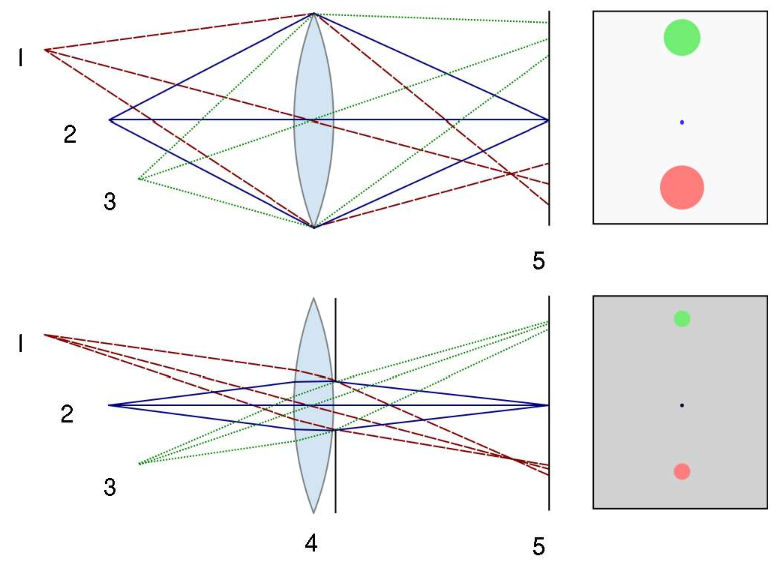
\includegraphics[scale=0.4]{images/3/diaphragm.png}
    \caption{Lente senza e con diaframma.}
\end{figure}

Ponendo un diaframma che chiude, in parte, l'apertura della lente, aumenta la profondità di campo. Questa è una via di mezzo tra le camere oscure e una normale fotocamera con lente
(cioè il punto 4 dell'elenco sopra): si usa solo una piccola parte della lente, i cerchi di confusione per i punti fuori fuoco saranno più piccoli, ma entrerà anche meno luce nel sensore.

\renewcommand{\thefigure}{3.24}
\begin{figure}[!h]
  \centering
    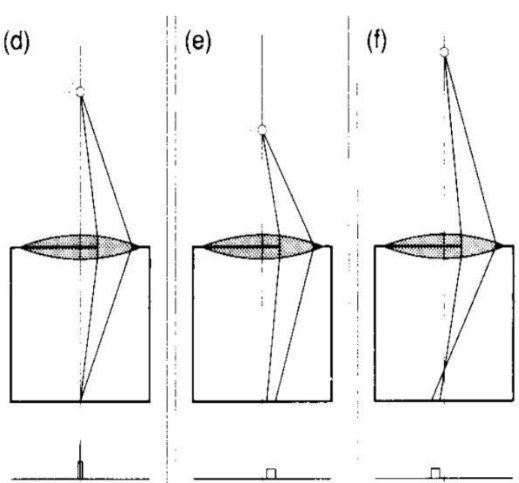
\includegraphics[scale=0.4]{images/3/partial_pinhole.png}
    \caption{Diaframma usato per fotografia plenottica.}
\end{figure}

Come possiamo sfruttare un diaframma per la fotografia plenottica? Lo vediamo qui sopra. Tenendo aperta solo un'estremità della lente, notiamo che se l'oggetto è più vicino
della distanza focale del sistema, il cerchio di confusione comparirà a destra del centro del sensore, se invece l'oggetto è più distante, il cerchio di confusione sarà a sinistra: riusciamo a
distinguere i due casi! L'immagine ci dà un'informazione sulla distanza dell'oggetto.

\subsubsection{Sistema con array di fotocamere stenopeiche}
Il sistema appena visto, con lente e diaframma, è però tecnicamente scomodo, e comunque non permette la messa a fuoco a posteriori. Come possiamo implementare la stessa idea, in modo più intelligente?
Mettiamo, dentro la fotocamera principale (dotata di lente), alla distanza in cui prima stava il sensore (cioè il fondo della fotocamera), una griglia forata.
Dietro questa griglia, staranno delle fotocamere stenopeiche.

\renewcommand{\thefigure}{3.25}
\begin{figure}[!h]
  \centering
    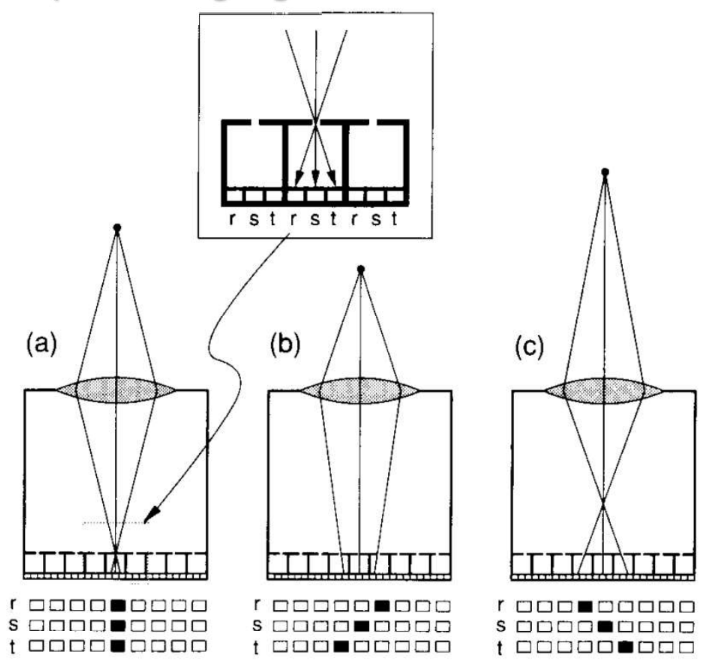
\includegraphics[scale=0.4]{images/3/pinhole_array.png}
    \caption{Sistema con array di camere oscure.}
\end{figure}

Ogni fotocamera stenopeica avrà tre pixel, $r$, $s$ e $t$. Se l'oggetto sarà a fuoco (fuoco standard dato dalle distanze oggetto-lente e lente-griglia forata), i raggi
si incontreranno proprio all'ingresso della camera oscura centrale, e si proietteranno sui pixel $r$, $s$ e $t$ della stessa.
Altrimenti, colpiranno il pixel $r$ di una certa fotocamera, il pixel $s$ di un'altra, e il $t$ di una terza.
Selezionando i pixel $r$, $s$ e $t$ dalle opportune fotocamere, possiamo ottenere un'immagine dove è a fuoco il punto a distanza standard, quello più lontano, o quello più vicino.
Per una risoluzione spaziale maggiore servono più pixel in ciascuna fotocamera stenopeica (più sotto-pixel ``fisici'' che vadano a formare un pixel ``logico''), per una maggiore precisione
nella stima della distanza servono tante fotocamere stenopeiche. Quindi c'è un compromesso tra le due cose.

\subsubsection{Microlenti}
Nella realtà, non si usa il sistema appena visto, ma si applica una matrice di microlenti sopra il sensore, che si occupano di dirigere i raggi di luce verso elementi fotosensibili
diversi in base alla direzione da cui provengono. Questa soluzione permette l'ingresso di più luce rispetto agli array di camere oscure.

\renewcommand{\thefigure}{3.26}
\begin{figure}[!h]
  \centering
    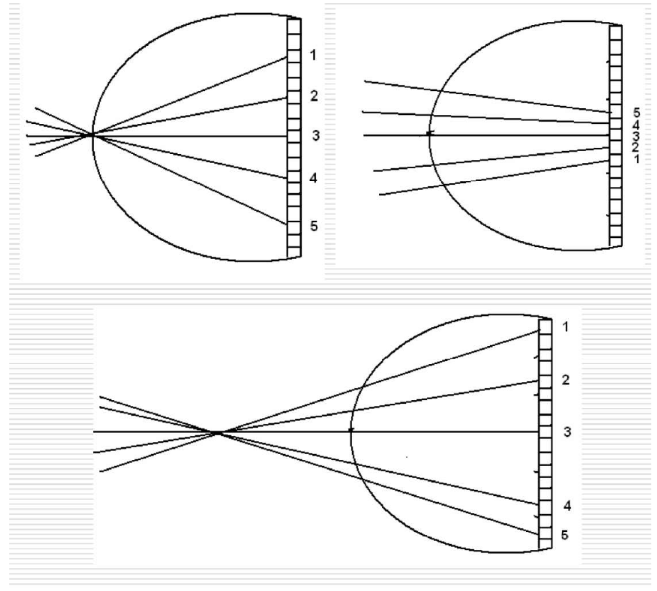
\includegraphics[scale=0.4]{images/3/microlenses.png}
    \caption{La microlente ridireziona i raggi in modo diverso se convergono su di essa, prima o dopo.}
\end{figure}

\subsubsection{Stima della profondità tramite utilizzo parziale della lente}
Facendo finta di posizionare un diaframma che blocchi una porzione della lente, possiamo ottenere immagini dell'oggetto
da diversi punti di vista: ad esempio, se prendo solo i dati portati dai raggi di luce che passano per la zona superiore della lente, avrò
un punto di vista rialzato dell'oggetto. Prendendo i dati in diversi modi analoghi a questo, si ottiene un insieme di immagini ``multiscopiche'' che possono essere usate
per costruire una mappa della profondità. Anche qui servono le microlenti sul sensore (altrimenti non ho modo di selezionare i pixel colpiti solo dalla luce che è passata in alto sulla lente).

\renewcommand{\thefigure}{3.27}
\begin{figure}[!h]
  \centering
    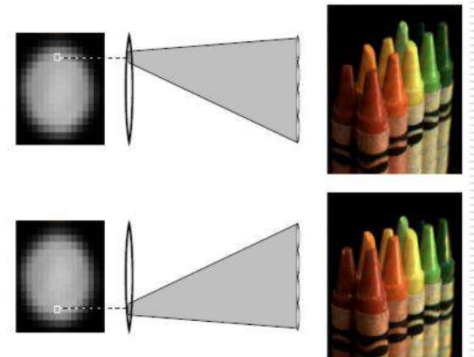
\includegraphics[scale=0.4]{images/3/depth.png}
    \caption{Nel primo caso abbiamo un punto di vista più rialzato che nel secondo caso.}
\end{figure}

\subsubsection{Stima della profondità con fotocamere stereoscopiche}
Il sistema basato sulle microlenti funziona meglio che quello che impiega fotocamere stereoscopiche, perché nel caso di queste ultime, potrebbero esserci zone occluse
in cui la ricostruzione della profondità non è possibile (non vengono viste da entrambe i sensori). Se la fotocamera è multiscopica (cioè usa le microlenti), allora ogni zona verrà vista da diversi sensori
e il tutto funzionerà molto meglio.

\renewcommand{\thefigure}{3.28}
\begin{figure}[!h]
  \centering
    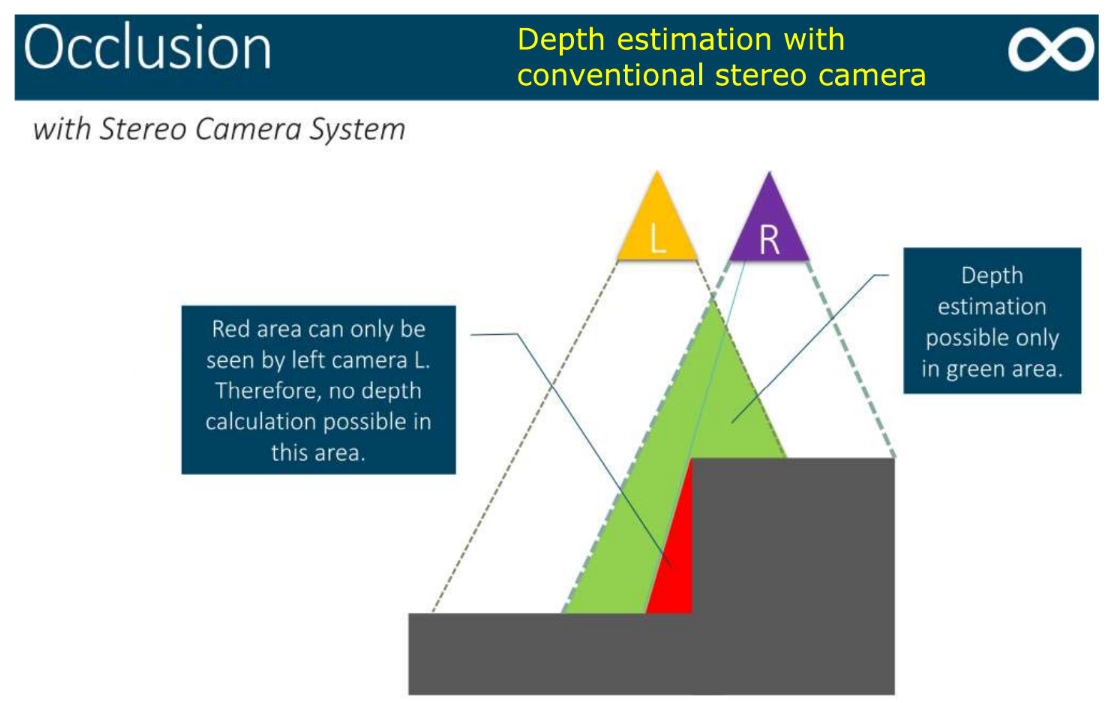
\includegraphics[scale=0.4]{images/3/stereo.png}
    \caption{Occlusione in una fotocamera stereoscopica.}
\end{figure}

\renewcommand{\thefigure}{3.29}
\begin{figure}[!h]
  \centering
    \includegraphics[scale=0.4]{images/3/multi.png}
    \caption{Problema risolto con una fotocamera multiscopica basata sulle microlenti.}
\end{figure}

\newpage
\subsubsection{Stima della profondità con il tempo di volo}
Si basa sull'emissione di un segnale luminoso infrarosso, e la valutazione del ritardo/sfasamento della sua versione riflessa che torna indietro (riflesso catturato da un pannello di sensori
apposito). Due possibili metodi: impulso di luce, oppure onda continua.
\par
\textbf{Impulso} (extra - non c'è sulle slide)

\renewcommand{\thefigure}{3.30}
\begin{figure}[!h]
  \centering
    \includegraphics[scale=0.4]{images/3/impulse_tof.png}
    \caption{Stima della profondità tramite impulso di luce.}
\end{figure}

\par
L'idea è che la fotocamera emette un impulso di luce infrarossa (il primo rettangolo del segnale \textit{Light Source}). Il segnale tornerà indietro dopo essere stato riflesso dall'oggetto
(primo rettangolo del segnale \textit{Reflection}). L'impulso riflesso potrà essere più o meno sovrapposto all'impulso originale. Il segnale \textit{C1} integra la porzione di luce riflessa
che arriva mentre l'impulso non si è ancora esaurito (notare che il primo rettangolo di \textit{C1}, infatti, è perfettamente allineato con l'impulso). Il risultato sarà un certo numero
di cariche $Q1$. Il segnale \textit{C2}, invece, integra la porzione di luce riflessa che arriva nell'intervallo tra un impulso e l'altro, e ci darà un altro numero di cariche $Q2$.
La distanza dell'oggetto sarà quindi
\[
d = \frac{1}{2} c \cdot \Delta t \Bigg(\frac{Q2}{Q1 + Q2}\Bigg).
\]
Chiaramente la minima distanza misurabile è 0 (caso in cui $Q1$ è massimo e $Q2 = 0$), la massima distanza è $0.5 \cdot c \cdot \Delta t$ (caso in cui $Q1 = 0$).

\par
\textbf{Onda continua}

\renewcommand{\thefigure}{3.31}
\begin{figure}[!h]
  \centering
    \includegraphics[scale=0.4]{images/3/cw_tof.png}
    \caption{Stima della profondità tramite onda continua.}
\end{figure}

\par
Ci sono quattro segnali di controllo, sfasati di $\pi / 2$ tra loro (sfasamento di 0, $\pi$, $\pi/2$ e $3\pi/2$ rispettivamente). Ognuno di essi integra la luce riflessa in un determinato intervallo.
Lo sfasamento tra luce riflessa e luce emessa può essere calcolato con
\[
\phi = arctan\Bigg(\frac{Q3-Q4}{Q1-Q2}\Bigg)
\]
e la distanza dell'oggetto sarà
\[
d = \frac{c}{4 \pi f} \phi.
\]
Poiché lo sfasamento si può misurare senza ambiguità solo nell'intervallo $[0, 2\pi]$, c'è una massima distanza rilevabile, che è chiaramente $d_{amb} = c/2f$.

\newpage

\section{Visualizzazione}
\subsection{Schermi}
Oggigiorno, gli schermi hanno risoluzioni più che accettabili, il problema rimane l'intervallo dinamico.

\subsubsection{Schermi LCD TFT}
I cristalli liquidi sono sostanze in una fase intermedia tra quella solida e quella liquida isotropica,
cioè quella in cui le molecole sono libere di orientarsi in qualsiasi direzione. Le molecole usate negli schermi sono calamitiche, cioè hanno forma allungata
(niente a che vedere con calamite e magnetismo). Le molecole sono formate da un corpo rigido (anelli aromatici) e delle code
mobili di carbonio e idrogeno. Grazie a questa struttura sono polari, e quindi reagiscono a un campo elettrico; inoltre
possono formare legami corpo-coda in modo da creare strutture di molecole orientate approssimativamente allo stesso modo.
Il loro comportamento dipende anche dalla temperatura: a basse temperature tendono a solidificarsi. Però, come detto,
a noi interessa una specifica mesofase, quella nematica. Nella realtà, le molecole usate non hanno una coda perfettamente
dritta, ma irregolare (sono molecole chirali). Se si osserva un blocco tridimensionale di molecole chirali,
si nota che a diverse profondità, la direzione in cui le molecole sono orientate cambia (anche senza campo elettrico, è proprio un fenomeno naturale dovuto alla chiralità).

\renewcommand{\thefigure}{4.1}
\begin{figure}[!h]
  \centering
    \includegraphics[scale=0.4]{images/4/tn_block.png}
    \caption{Blocco di cristalli liquidi chirali: notare il diverso orientamento a varie profondità.}
\end{figure}

Per costruire uno schermo, possiamo usare degli strati di allineamento (strati di plastica), che impongono alle molecole
una certo allineamento nello strato più in alto e in quello più in basso. Negli strati intermedi, si avrà
l'allineamento ad angolo variabile in base alla profondità. Questo è il principio degli schermi \textit{twisted nematic}.
In questi schermi, lo strato in alto è orientato parallelamente all'asse orizzontale schermo, mentre
quello in basso è perpendicolare allo stesso asse. Applicando un potenziale agli estremi del blocco di cristalli liquidi,
una rotazione nel piano trasversale allo schermo si aggiunge alla già presente rotazione naturale sul piano parallelo.
Questa rotazione aggiuntiva rende più o meno trasparenti le colonne di molecole (ne modifica la trasmittanza).

\renewcommand{\thefigure}{4.2}
\begin{figure}[!h]
  \centering
    \includegraphics[scale=0.6]{images/4/no_voltage.png}
    \caption{Sezione verticale di uno schermo: quando nessun potenziale è applicato, l'unica rotazione presente è quella sul piano parallelo allo schermo.}
\end{figure}

\renewcommand{\thefigure}{4.3}
\begin{figure}[!h]
  \centering
    \includegraphics[scale=0.6]{images/4/yes_voltage.png}
    \caption{Quando invece viene applicato un potenziale, c'è anche una rotazione sul piano trasversale allo schermo.}
\end{figure}

Un problema degli schermi a cristalli liquidi è che assorbono tantissima luce. La trasmittanza normalizzata
sale fino al 100\% (ovvio, è normalizzata rispetto al suo valore massimo), ma questo valore massimo è molto piccolo in realtà, perché la struttura dei cristalli
assorbe circa il 90\% della luce emessa dalla lampada di retroilluminazione.
Anche la trasparenza nulla è difficile da ottenere, quindi ottenere un nero assoluto è praticamente impossibile. La buona notizia, però, è che i valori di tensione da usare per comandare
i cristalli liquidi sono piuttosto bassi e quindi facilmente generabili.

\renewcommand{\thefigure}{4.4}
\begin{figure}[!h]
  \centering
    \includegraphics[scale=0.6]{images/4/trasmittance.png}
    \caption{Trasmittanza normalizzata in funzione della tensione applicata. Notare che non è perfettamente identica per i tre diversi colori (idealmente, vorremmo che lo fosse).}
\end{figure}

Un altro problema dei cristalli liquidi è il tempo di risposta molto alto (qualche millisecondo): bisogna ruotare fisicamente le molecole.
Inoltre, all'abbassarsi delle temperature, aumenta la viscosità della struttura, quindi i tempi salgono ancor di più. Temperature molto alte (sopra i 100°C) o molto basse (sotto lo zero)
causano la liquefazione o la solidificazione della struttura, ma non danneggiano permanentemente i cristalli liquidi.
\par
Cosa succede realmente quando applichiamo un potenziale ad una struttura di cristalli liquidi? Perché, se il potenziale è alto,
la struttura blocca la luce? Per rispondere a queste domande è necessario osservare la struttura dei vari strati
che compongono un intero schermo.
\newpage

\renewcommand{\thefigure}{4.5}
\begin{figure}[!h]
  \centering
    \includegraphics[scale=0.6]{images/4/lcd_layers.png}
    \caption{Struttura interna di uno schermo a cristalli liquidi.}
\end{figure}

Il secondo strato dal basso e quello superiore sono formati da due polarizzatori
con orientamento perpendicolare tra loro. Quando il potenziale applicato è nullo o basso, le molecole, che sono ruotate
solo sul piano orizzontale, modificano la polarizzazione della luce (che entra da sotto) in modo che, arrivata in cima,
essa sia polarizzata nella direzione compatibile con il polarizzatore superiore (detto ``analizzatore''). La luce quindi esce dallo
schermo, che ci appare chiaro. Se invece il potenziale applicato è alto, la rotazione sul piano verticale che esso induce impedisce
alle molecole di ruotare la polarizzazione della luce entrante, arrivata quindi in cima, la luce non avrà
una polarizzazione compatibile con l'analizzatore, e verrà bloccata.

\newpage
\renewcommand{\thefigure}{4.6}
\begin{figure}[!h]
  \centering
    \includegraphics[scale=0.4]{images/4/example_lcd.png}
    \caption{La luce viene polarizzata in modo compatibile con l'analizzatore solo quando non è applicato alcun potenziale.}
\end{figure}

La sorgente di luce era, un tempo, una lampada fluorescente, oggigiorno invece si usano dei LED. In ogni caso, è molto difficile ottenere
un'illuminazione uniforme uscente da una superficie, senza disperdere molta energia sottoforma di luce sprecata, quindi si rende necessario usare un diffusore.
Oggi, si usano spesso dei LED posti sulle cornici dello schermo, con dispositivi di plastica che si occupano di diffondere la luce uniformemente.
\par
Altri due strati sono costituiti dagli elettrodi di ossido di indio-stagno, che è trasparente. Sono loro a generare il potenziale che controlla lo schermo. Servono
tanti elettrodi quanti sono i pixel. Lo strato superiore di elettrodi è coperto da qualcosa che assomiglia a un fitro di Bayer.
\par
Ancora un problema di questi schermi: vi sono effetti indesiderati (errori di parallasse) se li osserviamo da una direzione non perpendicolare (in diagonale, quindi).
Per prima cosa, un certo punto dello schermo sarà illuminato da un raggio non perfettamente
verticale (l'immagine apparirà spostata di lato); in secondo luogo, il contrasto massimo raggiungibile dallo schermo
(rapporto tra massima e minima luminanza) cala rapidamente, se spostiamo lateralmente il nostro punto
di vista (comportamento molto anisotropico). Questo problema può essere mitigato, almeno in parte, con degli appositi dispositivi di plastica aggiuntivi.

\subsubsection{Schermi LCD IPS}
L'idea è di non piazzare gli elettrodi sopra e sotto, ma di metterli entrambi sotto. Questo riduce lo spessore
e quindi anche l'errore di parallasse. Le linee del campo elettrico, però, ora avranno forma a lobo.

\newpage
\renewcommand{\thefigure}{4.7}
\begin{figure}[!h]
  \centering
    \includegraphics[scale=0.4]{images/4/ips_field.png}
    \caption{Linee del campo elettrico in uno schermo IPS: gli elettrodi sono i due rettangolini posti sul vetro di sotto.}
\end{figure}

Funzionano in modo totalmente opposto agli schermi TN: qui, gli strati di allineamento sopra e sotto lo schermo
sono identici, quindi in assenza di campo elettrico lo schermo apparirà scuro (opaco alla luce).
Quando c'è un potenziale, le molecole si dispongono lungo i lobi delle linee del campo elettrico.

\renewcommand{\thefigure}{4.8}
\begin{figure}[!h]
  \centering
    \includegraphics[scale=0.4]{images/4/ips_switching.png}
    \caption{Principio del funzionamento di uno schermo IPS.}
\end{figure}

Nel centro della ``cella'' visibile nell'immagine, le molecole vengono ruotate sul piano orizzontale, quindi modificheranno
la polarizzazione della luce e lo schermo si illuminerà. Questo è il motivo per cui questi schermi si chiamano
\textit{In-Plane Switching}: la rotazione indotta dal campo non è più trasversale, ma complanare allo schermo.
Questo è un altro fattore che consente di ridurre lo spessore dello schermo: non serve costruirlo più grosso per
lasciare spazio alle molecole di orientarsi in verticale (in realtà, come si vede nell'immagine, proprio sopra gli elettrodi le molecole si orientano in verticale,
causando anche una riduzione della trasmittanza. Per mitigare questo effetto, si usano dei trucchi che non discutiamo).

\subsubsection{Schermi LCD IPS transflettivi}
Cercano di risolvere il problema della scarsa visibilità alla luce esterna (del sole). L'idea è di sfruttare
questa luce esterna per intensificare la luminosità dello schermo.

\renewcommand{\thefigure}{4.9}
\begin{figure}[!h]
  \centering
    \includegraphics[scale=0.4]{images/4/transflective.png}
    \caption{Schermo LCD transflettivo.}
\end{figure}

Si aggiungono due polarizzatori: sono lamine ``quarto d'onda'', cioè filtri che trasformano luce polarizzata linearmente
in luce polarizzata circolarmente, e viceversa. Servono per far sì che la polarizzazione della luce esterna sia concorde con quella della
lampada (entrambi i tipi di luce vengono filtrati due volte). Notare che la luce esterna passerà due volte attraverso
la struttura a cristalli liquidi! Questo significa che la sua intensità verrà ridotta due volte: non è un problema, perché di solito la luce esterna è molto forte.
\par
Il problema di questi schermi è che i due nuovi polarizzatori assorbono luce, quindi serve una lampada ancora più
forte per i casi in cui la luce ambientale è scarsa: aumenta il surriscaldamento ed il consumo di energia.

\subsubsection{Schermi LCD a colori}
Per ottenere uno schermo a colori, si applica una sorta di filtro di Bayer.
\par
Nel diagramma di cromaticità, vediamo rappresentati tutti i colori che noi possiamo percepire. Sugli assi ci sono delle quantità
non meglio definite, che prendono valori nell'intervallo $[0, 1]$: queste quantità ci permettono di rappresentare
i colori in questo strano modo. Sul bordo della curva stanno i colori puri, muovendosi verso l'interno
ci sono le combinazioni dei vari colori. Localizzati sul diagramma i punti corrispondenti ai colori verde, rosso e blu dei
tasselli del filtro di Bayer che usiamo, il nostro schermo potrà rappresentare tutti e soli i colori che stanno all'interno del triangolo risultante (sono pochi, rispetto al totale!).

\renewcommand{\thefigure}{4.9}
\begin{figure}[!h]
  \centering
    \includegraphics[scale=0.4]{images/4/chromaticity.png}
    \caption{Diagramma di cromaticità standard.}
\end{figure}

\subsubsection{Retroilluminazione a LED}
Poiché i colori dei LED dipendono da temperatura, polarizzazione, e altri fattori, servono dei sensori di feedback per far
sì che i LED siano regolati in modo da produrre una luce risultante bianca.

\renewcommand{\thefigure}{4.10}
\begin{figure}[!h]
  \centering
    \includegraphics[scale=0.4]{images/4/feedback.png}
    \caption{Sistema retroazionato per il controllo della retroilluminazione.}
\end{figure}

Digressione sulla luce bianca: la luce bianca dovrebbe avere densità spettrale di potenza piatta (come il rumore bianco), invece non è così. I LED bianchi sono LED blu con apposita copertura.
Grazie al metamerismo, diverse combinazioni di colori vengono percepite da noi come ``bianco''.

\subsubsection{Schermi LCD a doppio pannello}
Raddoppia la profondità del colore (da 8 bit per pixel a 16), ma si riduce la (già bassa) trasparenza dello schermo.
Il contrasto migliora molto. Sono due schermi in cascata: la trasmittanza totale sarà il prodotto delle
trasmittanze dei singoli schermi. Quindi se voglio ottenere una trasmittanza totale $Y$, dovrò raggiungere una trasmittanza di $\sqrt{Y}$ su ciascun pannello.
\par
All'atto pratico, questi schermi migliorano molto la resa del nero e dei grigi molto scuri. Rappresentare colori molto chiari non è così facile, a causa dell'altissima assorbenza di luce.

\renewcommand{\thefigure}{4.11}
\begin{figure}[!h]
  \centering
    \includegraphics[scale=0.4]{images/4/dual_lc_example.png}
    \caption{Immagine medica visualizzata su schermo a doppio pannello (sinistra) e schermo a pannello singolo (destra). Il contrasto è molto migliore a sinistra.}
\end{figure}

\subsubsection{Schermi ibridi LED + LC}
Sono schermi basati su quelli a doppio pannello, ma dove uno dei pannelli è sostituito con una matrice
di LED, che vengono usati per rappresentare una versone semplificata del contenuto dell'immagine.
La retroilluminazione, quindi, non è più uniforme, ma è modulata nello spazio, in base all'intensità dei vari punti dell'immagine.

\renewcommand{\thefigure}{4.12}
\begin{figure}[!h]
  \centering
    \includegraphics[scale=0.4]{images/4/led_lc_structure.png}
    \caption{Struttura di uno schermo ibrido.}
\end{figure}

Perché non usare solo una matrice di LED per visualizzare l'immagine, e basta? In realtà questo già si fa, ad esempio negli schermi usati in grandi eventi e cose del genere
(megaschermi allo stadio e ai concerti, eccetera), ma per altre applicazioni, dove gli schermi devono essere piccoli e osservati da vicino, non va bene,
perché non siamo in grado di produrre LED piccoli come i pixel.
\par
All'atto pratico, la matrice di LED si accende per mostrare una forma grezza dell'immagine. Il pannello a cristalli liquidi, invece, rifinisce i dettagli, bloccando
la luce dei LED laddove non deve passare. Tra il pannello di LED e quello di cristalli, ci deve essere anche un diffusore, per sparpagliare la luce
e impedirci di vedere punti particolarmente chiari laddove stanno i LED più luminosi.

\renewcommand{\thefigure}{4.13}
\begin{figure}[!h]
  \centering
    \includegraphics[scale=0.4]{images/4/led_lc_outline.png}
    \caption{Immagine desiderata e configurazione necessaria a rappresentarla.}
\end{figure}

Questa soluzione funziona ed è usata nella pratica. Richiede un processamento dell'immagine
più accurato per poter comandare il pannello LC nel modo giusto. Un problema che si manifesta
è che qualche raggio di luce prodotto dai LED più luminosi può riflettersi, invece che entrare nel pannello LC,
tornare sulla matrice di LED, ed essere nuovamente riflesso altrove, intaccando altri pixel. Si può risolvere con dei
paraluce obliqui intorno ai vari LED, cosicché i raggi di ritorno vengano riflessi nuovamente sul pixel corretto.
\par
L'idea di base nel processamento dell'immagine rimane simile a quella degli schermi LCD a doppio pannello:
$Y = \sqrt{Y} \cdot \sqrt{Y}$. Poiché la matrice dei LED ha una risoluzione molto più bassa di quella del pannello frontale a cristalli liquidi, bisognerà
sottocampionare l'immagine $\sqrt{Y}$ (con annesso filtraggio passa-basso), e poi ci saranno alcuni altri fattori che entreranno in gioco.
Vediamoli:
\begin{itemize}
    \item $I_L$ è la $\sqrt{I}$ passata in un filtro passa-basso;
    \item $r_1^{-1}(I_L)$ è la $I_L$ sottocampionata, usata per comandare i LED. I suoi pixel hanno forma esagonale per massimizzarne la densità. Serve processamento
    accurato per mappare la griglia di pixel quadrati in questa griglia di pixel esagonali;
    \item $p1 \ast I_L$ è un modello dell'immagine mostrata dai LED e passata attraverso il diffusore, e tutti gli altri strati e dispositivi di plastica che stanno tra la
    matrice di LED e il pannello a cristalli liquidi (strati non mostrati nell'immagine, per semplicità). È decimata. (Perché? Dal diagramma a blocchi non sembrerebbe)
    \item Dividiamo poi $I$ per quest'ultimo modello (cioè dividiamo $I$ per ciò che viene visualizzato all'ingresso del pannello LC). Otteniamo una versione più
    contrastata dell'immagine originale.
    \item Il pannello LC verrà infine comandato da $r_2^{-1}(\frac{I}{p_1 \ast I_L})$.
    Cosa sia $r_2^{-1}()$ rimane un mistero.
\end{itemize}

\renewcommand{\thefigure}{4.14}
\begin{figure}[!h]
  \centering
    \includegraphics[scale=0.4]{images/4/hybrid_processing.png}
    \caption{Catena di processamento necessaria in uno schermo ibrido.}
\end{figure}

\subsubsection{Schermi a LED}
La luminanza di uno schermo LCD si attesta sulle 400-500 cd/m2. I LED possono arrivare fino a 1000.
I MicroLED in teoria fino a 100000.
\par
Gli schermi a LED possono essere monolitici: singolo chip con il display da applicare su un altro circuito integrato che lo controlla.
Problema: le tecnologie per realizzare i due chip sono diverse, con conseguente caratteristiche termiche diverse tra i due strati.
L'espansione termica può danneggiare lo schermo. Non efficiente perché serve generare chip grande per il display, che costa molto.
La possibilità più interessante è quindi quella di produrre un wafer di MicroLED, lo spezzo in diverse parti e pongo le parti sopra al circuito di controllo (non molto chiaro perché questo sia meglio).
Più complesso da realizzare.

\subsubsection{Schermi OLED}
LED organici. Funzionano spostando cariche tra diversi livelli di energia consentiti nei vari materiali di cui sono composti. I materiali sono molecole organiche, non semiconduttori.
L'anodo (ITO) è trasparente ed emette lacune. In realtà le lacune sono emesse dal polimero conduttivo.
Il catodo non è trasparente, e possono essercene più di uno, per generare più elettroni e quindi più luce.
Il polimero emittente genera elettroni. HOMO e LUMO corrispondono alla banda di valenza e di conduzione.
Se i livelli di energia HOMO e LUMO sono correttamente distanziati, quando gli elettroni si combinano con le lacune
vengono generati i fotoni. L'efficienza di questi schermi OLED si attesta intorno al 10\%: meglio degli LCD ma molto peggio degli schermi a LED,
che arrivano anche al 70\%. In base al materiale usato in ciascun pixel, possiamo ottenere nativamente luce blu, rossa o verde. Lo spettro
non è proprio precisissimo, ma è comparabile al filtro Bayer. L'OLED permette di costruire schermi flessibili.

\renewcommand{\thefigure}{4.15}
\begin{figure}[!h]
  \centering
    \includegraphics[scale=0.4]{images/4/oled.png}
    \caption{Struttura di un pixel OLED.}
\end{figure}

Gli schermi OLED al momento dominano il mercato, anche se gli schermi a LED avrebbero caratteristiche migliori! I LED a semiconduttore sono
più efficienti energeticamente, hanno una durata più lunga, e possono emettere più potenza, quindi permettono di costruire schermi con un più ampio intervallo dinamico. Ma ancora
non siamo in grado di produrre LED sufficientemente piccoli e in grado di generare il nero assoluto.
\par
Indirizzamento passivo a matrice: abbiamo una matrice di OLED. Le righe vengono scansionate
una alla volta: quella in scansione viene portata a massa. L'informazione sta sulle colonne. Quando una linea è a massa,
solo i suoi OLED corrisponenti alle colonne attive si illumineranno. Problema: ogni riga emetterà luce solo per un breve periodo,
durante il quale le altre sono spente. Non vedrò mai l'immagine intera! La vedrò a righe. In realtà ci salva
la persistenza delle immagini sulla retina. La luminanza media sarà quella di un singolo pixel divisa per il numero di righe: è molto bassa.

\renewcommand{\thefigure}{4.16}
\begin{figure}[!h]
  \centering
    \includegraphics[scale=0.24]{images/4/pmoled.png}
    \caption{Indirizzamento passivo a matrice.}
\end{figure}

Indirizzamento attivo a matrice: c'è un circuito complesso per ogni OLED, che gli permette di stare attivo anche
quando l'indirizzamento passa a una riga successiva. Quando il segnale di scansione si abbassa, il transistor nella zona verde
si apre, carica il condensatore in base al segnale del dato, a quel punto si apre il transistor della zona rossa e l'OLED
si illumina. Quando il segnale di scansione si rialza, il condensatore si occupa di mantenere attivo il transistor della zona rossa.

\renewcommand{\thefigure}{4.17}
\begin{figure}[!h]
  \centering
    \includegraphics[scale=0.4]{images/4/amoled_cell.png}
    \caption{Indirizzamento attivo a matrice.}
\end{figure}

\subsubsection{Schermi a punti quantici}
I punti quantici sono particelle fluorescenti così piccole da risentire di effetti quantistici. Hanno effetti fluorescenti differenti in base alla loro dimensione e al materiale,
e quindi quando esposti a luce a spettro uniforme/blu, generano luce con spettro molto sottile e preciso.

\subsubsection{TV a confronto}
Nelle TV \textbf{OLED}, non è vero che ogni OLED emette luce di un certo colore: lo spettro emesso è ampio e c'è comunque un filtro di Bayer.
Di conseguenza, si perde efficienza. A differenza della struttura di un OLED vista nel grafico precedente, c'è un solo
catodo ma vari strati di materiale organico emittente, per migliorare l'efficienza. Ogni OLED quindi è un subpixel con intensità
diversa (subpixel perché poi 4 OLED contribuiscono, col filtro di Bayer, a creare un vero e proprio pixel a colori).
Il filtro contiene anche una banda trasparente per far passare più luce (cioè aggiungere un po' di bianco ai colori), in
modo da migliorare la resa per le zone più chiare.

\renewcommand{\thefigure}{4.18}
\begin{figure}[!h]
  \centering
    \includegraphics[scale=0.3]{images/4/tv_oled.png}
    \caption{TV OLED.}
\end{figure}

Le TV \textbf{LCD + QD} (QLED) sono LCD con una retroilluminazione blu a LED, poi c'è uno strato di punti quantici (sempre nell'ambito
della retroilluminazione), che purifica la retroilluminazione generando un rosso, un blu e un verde con spettri molto precisi, ma questi fasci di luci sono ancora mescolati
(quindi formano un unico fascio bianco). Serve quindi comunque un filtro di Bayer per generare i colori veri e propri. Le posizioni sullo 
schermo in cui questi colori verranno visualizzati sono controllate dai cristalli liquidi (con tutti i loro problemi).

\renewcommand{\thefigure}{4.19}
\begin{figure}[!h]
  \centering
    \includegraphics[scale=0.25]{images/4/tv_qled.png}
    \caption{TV QLED.}
\end{figure}

Le TV a \textbf{punti quantici fotoemissivi} sono in fase di sviluppo. Come le QLED, usano una retroilluminazione blu, ma
i punti quantici ora sostituiscono il filtro di Bayer. Quindi, il pannello LC riceve e modula semplicemente la retroilluminazione
blu, che poi, poco prima di raggiungere il vetro frontale dello schermo, si imbatte in un array di punti quantici, che genera i veri colori (molto precisi). Non c'è più il filtro di Bayer.

\renewcommand{\thefigure}{4.20}
\begin{figure}[!h]
  \centering
    \includegraphics[scale=0.25]{images/4/tv_pe_qd.png}
    \caption{TV a punti quantici fotoemissivi.}
\end{figure}

Le TV a \textbf{punti quantici elettroemissivi} saranno lo stadio di sviluppo ancora successivo. Sfruttano dei punti quantici
sensibili ad un flusso di elettroni, invece che alla luce. Non ci sarà più una retroilluminazione, ma semplicemente un catodo
che emetterà elettroni, questi colpiranno lo strato di punti quantici, che genereranno quindi la loro luce.

\renewcommand{\thefigure}{4.21}
\begin{figure}[!h]
  \centering
    \includegraphics[scale=0.25]{images/4/tv_ee_qd.png}
    \caption{TV a punti quantici elettroemissivi.}
\end{figure}

Le TV a \textbf{microLED con punti quantici} saranno un'alternativa. Al momento è difficile costruire microLED con colori diversi
in posizioni diverse, quindi la soluzione potrebbe essere generare luce blu modulata spazialmente con dei microLED blu, dopodiché
usare un pannello a punti quantici per rendere rossi o verdi i pixel che devono esserlo.

\renewcommand{\thefigure}{4.21}
\begin{figure}[!h]
  \centering
    \includegraphics[scale=0.3]{images/4/tv_uled_qd.png}
    \caption{TV a microLED con punti quantici.}
\end{figure}

\subsubsection{Dolby Vision}
\begin{itemize}
    \item \textit{Wide Color Gamut}: possibilità di produrre la più grande porzione possibile dello zoccolo dei colori.
    \item \textit{Perceptual Quantizer}: è la funzione di trasferimento proposta in questo documento, unisce problemi tecnologici con elementi della visione umana.
\end{itemize}

Al momento, lo stato dell'arte per quanto riguarda i segnali video si riferisce ancora agli schermi a tubo catodico, che erano in grado di produrre dei buoni neri,
ma erano molto scarsi dal punto di vista dei bianchi, avendo una luminanza massima di soli 100 nit.
Il comportamento nella resa dei colori è ancora legato al vecchio standard ``ITU-R Recommendation BT.709'', anch'esso tarato sulla capacità di riproduzione dei colori degli schermi CRT.
\par
Un lato positivo dei CRT era che si comportavano tutti allo stesso modo, perché era possibile calibrarli uniformemente. Quindi
le immagini visualizzate erano coerenti tra tutti i diversi schermi (che aderivano agli standard).
Un altro lato positivo dei CRT è che la loro risposta non è lineare.
La relazione nonlineare dei CRT è $y = x^{\gamma}$, con $\gamma = 2.4$. Per coincidenza, questa risposta è molto simile all'inversa di quella dell'occhio umano.

\renewcommand{\thefigure}{4.22}
\begin{figure}[!h]
  \centering
    \includegraphics[scale=0.45]{images/4/gamma_barten.png}
    \caption{Correzione di gamma quantizzate con 10 bit (curva rossa) e 15 bit (curva blu). \textbf{Non 8 o 10!} È un errore.}
\end{figure}

Nella correzione di gamma, cioè il postprocessamento delle immagini acquisite tramite la funzione inversa della risposta dei CRT,
se usiamo una quantizzazione con ``pochi'' bit (curva rossa), e quindi ci teniamo al di sopra della curva della soglia del contrasto secondo Barten,
differenze dovute ad errori di quantizzazione saranno percettibili: male!
Se invece usiamo più bit per la quantizzazione (curva blu), possiamo rendere impercettibili gli errori di quantizzazione, però tale quantizzazione
sarà più dispendiosa. Bisogna anche riadattare tutti i dispositivi che ora lavorano con pochi bit
affinché possano lavorare con più bit. Inoltre, l'intervallo sull'asse $x$ è ancora quello dei CRT, ma ora possiamo andare ben oltre i 100 nit. Appare chiaro che adattare
la correzione di gamma alle tecnologie e alle esigenze moderne sarebbe inefficiente e certamente non ottimale.
\par
Vogliamo quindi progettare due nuove funzioni di trasferimento che mettano in relazione la fotocamera con l'immagine acquisita (OETF),
e l'immagine acquisita con lo schermo (EOTF). La EOTF non era un problema con i CRT,
perché di default si comportavano allo stesso modo! Quindi fino a poco tempo fa, solo la OETF era standardizzata.
OETF + EOTF = OOTF (non è una vera somma, è da intendere come cascata delle due funzioni di trasferimento).
Sarebbe bello che la OOTF fosse unitaria, cioè che facesse visualizzare sullo schermo un'immagine che noi poi potremmo percepire esattamente come se fosse reale.

\renewcommand{\thefigure}{4.23}
\begin{figure}[!h]
  \centering
    \includegraphics[scale=0.4]{images/4/bwh.png}
    \caption{Esperimento per determinare la luminanza ritenuta buona per il nero, il bianco e gli \textit{highlight}.}
\end{figure}

\textit{Highlight}: dettagli la cui intensità va oltre il bianco (riflessi e sorgenti di luce).
C'è un compromesso tra soddisfazione degli utenti e complessità realizzativa (accontentiamo il 90\% persone, altrimenti dobbiamo
creare schermi troppo complessi e costosi per raggiungere intensità così estreme).
\par
Vogliamo dunque progettare una funzione di trasferimento per lo schermo, che permetta di stare sotto la curva di Barten (vista prima) nell'intero nuovo intervallo di luminanze
riproducibili dai nostri schermi moderni. Una correzione di gamma a 10 bit non è più sufficiente a stare sotto la curva di Barten.

\renewcommand{\thefigure}{4.24}
\begin{figure}[!h]
  \centering
    \includegraphics[scale=0.45]{images/4/pq.png}
    \caption{Grafico della nuova OETF, denominata \textit{Perceptual Quantizer}.}
\end{figure}

Si nota che un PQ a 12 bit basta a stare sotto la curva di Barten, e l'andamento è molto simile a questa curva (non più dritto). Una correzione di gamma dovrebbe avere
addirittura 15 bit per poter stare sotto la curva di Barten nell'intero intervallo sull'asse orizzontale! Per gli ambiti applicativi in cui 12 bit di quantizzazione sono troppi,
Dolby definisce anche il PQ a 10 bit, che pur stando sopra la curva di Barten, permette di avere errori di quantizzazione così piccoli da essere impercettibili.
\par
In questi standard sono presenti anche metadati, così il display si può adattare ai vari tipi di segnale che va a rappresentare (chiaramente
i produttori di display devono adattarsi, e cominciare a produrre schermi che supportino questa funzionalità).

\subsubsection{Recommendation ITU-R BT.2100-2}
Cerca di standardizzare i parametri per la produzione di immagini destinate alla televisione HDR.

\subsubsection{Report ITU-R BT.2390-9}
Descrive come un sistema di processamento delle immagini HDR debba essere realizzato.

\subsubsection{Altre tecnologie per la realizzazione di schermi}
\begin{itemize}
    \item Schermi transflettivi: ne abbiamo già parlato. Sono quelli che sfruttano anche la luce ambientale. Ancora in lavorazione.
    \item Pixel elettroforetici: usati nei lettori di eBook. Anche noto come ``inchiostro elettronico'', usa gli stessi pigmenti
    usati nell'editoria. Lo schermo è formato da tante microcapsule, che contengono un po' di particelle bianche, che hanno carica
    positiva, e un po' di particelle nere, che hanno carica negativa. Un potenziale applicato da degli elettrodi sottostanti lo schermo
    muove su e giù le particelle e crea pixel bianchi, neri o grigi. Problema: c'è materiale da spostare fisicamente, dunque gli schermi
    hanno tempi di risposta molto alti. Non adatto per realizzare schermi per la visualizzazione di video. Sfruttano la luce ambientale senza i problemi degli LCD transflettivi.
    \item Pixel elettrofluidici: sfruttano gli effetti causati da un campo elettrico e un liquido su una superifice idrofobica.
    Sono realizzati mettendo dell'olio colorato su una superficie
    idrofobica, sopra l'olio ci sarà dell'acqua. Applicando un potenziale adeguato, posso spostare la goccia d'olio in modo che
    sia molto piatta e splamata su tutto il pixel, oppure molto gobba e messa in un angolino. In altre parole, l'angolo tra la superficie della goccia e la superficie idrofobica, normalmente legato alle tensioni 
    superficiali del liquido in stati diversi (equazione di Young), è qui legato anche alla differenza di potenziale applicata. Chiaramente, ciò cambierà le
    proprietà del pixel: quando la goccia d'olio (supponiamolo blu) è spalmata su tutto il pixel, il pixel apparirà blu, quando invece è relegata in un
    angolino, il pixel apparirà bianco (non colorato). I tempi di risposta sono migliori di quelli dell'inchiostro elettronico, ed è possibile costruire
    pixel riflettenti/transflettivi usando questa tecnologia.
\end{itemize}

\subsection{Proiettori}

\subsubsection{LCD/LCP}
Una sorgente di luce genera una luce bianca, che viene scomposta nelle componenti RGB da degli specchi dicroici. Le tre componenti
arrivano poi a dei pannelli LC, che le modulano spazialmente in base all'immagine da rappresentare. Un cubo dicroico compone poi le tre
componenti dell'immagine e le trasmette sulla superficie su cui si desidera proiettare.
\par
I problemi, qui, sono quelli tipici dei pannelli LC: assorbono molta luce! Siccome la sorgente luminosa di un proiettore è molto forte,
i pannelli LC assorbiranno tanta potenza, e quindi si scalderanno molto, perdendo in prestazioni e degradandosi.
Inoltre, la resa di neri e bianchi è poco convincente.

\renewcommand{\thefigure}{4.25}
\begin{figure}[!h]
  \centering
    \includegraphics[scale=0.45]{images/4/lcd_projector.png}
    \caption{Struttura di un proiettore a cristalli liquidi.}
\end{figure}

\subsubsection{LCoS}
\textit{Liquid Crystal on Sylicon}. Sono dei proiettori basati su pannelli a cristalli liquidi riflettenti: hanno degli specchi posti tra il substrato di silicio e il pannello
LC, che riflettono la luce della lampada (che arriva da davanti al pannello LC, non da dietro) e anche quella ambientale.
\par
Vantaggi: il pannello LC può essere più sottile, perché viene attraversato due volte, quindi
l'attenuazione sarà buona comunque. Si guadagna, di conseguenza, nei tempi di risposta e nel contrasto ottenibile (come negli schermi a doppio pannello di cristalli liquidi,
migliorano molto i neri). Ma soprattutto, tutta l'elettronica di controllo sta fuori dal percorso della luce! L'apertura, quindi, è molto alta. Non servono polarizzatori, se ne occupano i
\textit{beam splitter}.

\renewcommand{\thefigure}{4.26}
\begin{figure}[!h]
  \centering
    \includegraphics[scale=0.55]{images/4/lcos_path.png}
    \caption{Il percorso della luce in un proiettore LCoS.}
\end{figure}

Dentro le celle in cui stanno i pannelli LC:
\begin{enumerate}
    \item un fascio di luce rossa, blu o verde entra (questo sistema è replicato tre volte nel proiettore, una per ogni componente della luce);
    \item colpisce un \textit{beam splitter};
    \item viene direzionato sul pannello LC (\textit{SXRD panel});
    \item gli specchi messi tra pannello e silicio la rimandano indietro;
    \item colpisce di nuovo il \textit{beam splitter}, ma stavolta, a causa della polarizzazione acquisita, ci passa attraverso;
    \item si dirige verso il punto di output.
\end{enumerate}

\subsubsection{Come rendere un proiettore LC più economico}
Sia qui che nelle soluzioni basate su cristalli liquidi, si potrebbe realizzare un proiettore
più economico usando un solo pannello LC impiegato sequenzialmente, prima per modulare la componente rossa, poi quella verde e
infine quella blu. Se alternate con velocità adeguata (almeno 25 fps), l'occhio percepisce il tutto come un'unica immagine.
Per fare una cosa del genere, serve una filtro rotante che dia il colore giusto al fascio di luce che entra nel pannello LC.
Il pannello LC deve essere sincronizzato, perché dia la modulazione spaziale necessaria a ciascuna componente luminosa
nel momento giusto.
Problema: c'è un componente (il filtro rotante) in movimento meccanico (più possibilità che si rompa), ma è solo una piccola rotellina. Incrociamo le dita e speriamo bene.

\subsubsection{Proiettori a microspecchi}
Questa è la teconologia dominante. Invece di un pannello a cristalli liquidi, si usa un pannello di microspecchi basculanti in diagonale.
Per visualizzare un pixel chiaro, oriento lo specchio in modo che rifletta appieno la luce sulla lente del sistema ottico
di output. I microspecchi sono simili a interruttori binari: o puntano contro la lente, o puntano da un'altra parte.
Se ho bisogno di intensità intermedie, devo alternare i due orientamenti velocemente con un \textit{duty cycle} adeguato.

\subsubsection{Vobbulazione}
Un problema dei proiettori è che un proiettore ad alte risoluzioni (ad esempio, 4K) è molto costoso, rispetto ad uno schermo di uguale risoluzione.
Questo perché è estremamente costoso produrre versioni ad alta risoluzione delle strutture fisiche usate nei proiettori.
\par
Entra in gioco ora la vobbulazione: un chip apposito scompone l'immagine 4K da proiettare in due o quattro immagini a più bassa risoluzione, che interlacciate diano l'immagine originale.
Il proiettore poi proietta in modo alternato queste immagini, con uno scostamento diverso per ciascuna (scostamento realizzato spostando meccanicamente la lente),
in modo che noi, grazie alla persistenza sulla retina delle varie immagini proiettate, possiamo percepire l'immmagine originale ad alta risoluzione.

\subsubsection{Sorgenti di luce}
Le lampade ad arco, molto usate nei proiettori, sono fragili, durano poco e sono poco efficienti. Come migliorare le sorgenti di luce? Vediamo.
\par
Per proiettori che non necessitano di alta potenza (quelli portatili) possiamo usare dei LED, per gli altri bisogna usare i laser (soluzione complicata).
\par
C'è una soluzione intermedia, che prevede l'uso di un LED rosso e di un laser blu, perché LED rossi ad alta potenza sono realizzabili abbastanza facilmente, e lo stesso vale per i laser blu.
La luce blu del laser viene divisa in blu e verde da una rotella. Lenti e specchi appropriati si occupano di convogliare la luce sui microspecchi.

\renewcommand{\thefigure}{4.27}
\begin{figure}[!h]
  \centering
    \includegraphics[scale=0.25]{images/4/casio.jpg}
    \caption{Soluzione intermedia progettata da Casio.}
\end{figure}

Problema delle sorgenti a laser: rumore granulare (\textit{speckle noise}), dovuto alla luce incidente su superfici non omogenee. Generalmente, non è un problema per la luce ambientale, perché
essa è incoerente (ha diverse frequenze e fasi), quindi gli effetti si disperdono nel disordine della luce naturale.
Quando si usa una sorgente omogenea, però, gli effetti si sommano tra loro e sono chiaramente visibili (ad esempio, puntando un puntatore laser contro il muro).

\subsection{Schermi e proiettori 3D}
\subsubsection{Stereoscopia}
È la tecnica alla base del 99\% delle soluzioni adottate nel campo del 3D. Abbiamo due immagini e dobbiamo trovare il modo di mostrarle in modo adeguato
agli occhi dello spettatore. Le tecniche si dividono in:
\begin{itemize}
    \item stereoscopiche a visione diretta (con occhiali);
    \item autostereoscopiche a visione diretta (senza occhiali);
    \item basate su dispositivi che si mettono in testa (non ci interessano).
\end{itemize}
Un problema di cui tutte le tecniche basate sulla stereoscopia soffrono è dovuto alla non congruenza tra il punto di convergenza ed il punto di messa a fuoco degli occhi,
cioè: se guardo un'immagine di una lunga strada con un edificio in fondo, lo sguardo converge su un oggetto che sarebbe lontano, ma in realtà sto mettendo a fuoco
lo schermo che ho davanti. Il punto di messa a fuoco è fisso, mentre il punto di convergenza cambia in base alla profondità a cui si trova, nell'immagine riprodotta sullo schermo, l'oggetto su cui stiamo rivolgendo
la nostra attenzione. Questo può causare malessere e mal di testa: meglio non rappresentare oggetti troppo lontani.

\subsubsection{Stereoscopia a visione diretta}
Il \textbf{primo approccio} sfrutta la multiplazione basata sul colore (quella con occhiali a lenti rosse e blu). Non funziona bene per due ragioni:
\begin{enumerate}
    \item il \textit{cross-talk}: l'immagine che dovrebbe arrivare solo all'occhio destro giunge anche a quello sinistro, e viceversa. Questo è dovuto al fatto
    che le due lenti non filtrano perfettamente le immagini;
    \item se uso dei colori per codificare ciò che va a ciascun occhio, perdo la possibilità di usare effettivamente quei colori nell'immagine.
\end{enumerate}
\par
Esiste un affinamento di questo approccio, che sfrutta il fatto che i nostri coni hanno una percezione dei colori fondamentali piuttosto grezza (la
risposta ha una forma a campana piuttosto ampia). Posso quindi codificare i vari colori nelle due immagini usando diverse sotto-bande dei tre colori fondamentali. Dopodiché,
gli occhiali filtreranno l'immagine complessiva in modo che un occhio veda un gruppo di sottobande (che costituiscono una delle due immagini), e l'altro veda il secondo gruppo.

\renewcommand{\thefigure}{4.28}
\begin{figure}[!h]
  \centering
    \includegraphics[scale=0.35]{images/4/3d_cmux.png}
    \caption{Versione affinata del sistema stereoscopico basato sulla multiplazione del colore.}
\end{figure}

Questa tecnica funziona bene e può essere semplificata usando un solo proiettore invece che due (che sono costosi, e vanno calibrati in modo che puntino
entrambi in modo coerente sullo schermo): bisogna usare una rotella che filtri l'immagine facendo passare i due gruppi di sotto-bande dalla lampada all'ottica in modo alternato.
\par
Il \textbf{secondo approccio} si basa sulla multiplazione tramite la polarizzazione della luce. Posso ad esempio usare una polarizzazione lineare a 45° per l'immagine
destinata all'occhio sinistro, e una polarizzazione lineare a 135° per l'altra. Gli occhiali dovranno avere delle lenti che contengono adeguati filtri analizzatori. Non è molto
comoda come soluzione, perché è necessario che la testa dello spettatore sia sempre verticale, pena un elevato \textit{cross-talk}. Molto meglio usare la polarizzazione circolare, con versi differenti (orario e antiorario). Al posto dei filtri di che separavano le sotto-bande di colori, usiamo due
filtri polarizzatori, e serve un telo che preservi la polarizzazione. Questo metodo può anche essere usato per realizzare uno schermo 3D. Come? Vediamo.
\par
Bisogna generare due immagini che abbiano risoluzione dimezzata rispetto alle due immagini originali, cioè devono avere metà delle righe. La
qualità quindi sarà degradata (perdo risoluzione orizzontale). Serve poi uno speciale schermo che, oltre ai soliti polarizzatore e analizzatore degli LCD, abbia
dei pannelli in più che generino la polarizzazione circolare. Questi pannelli sono:
\begin{enumerate}
    \item una lamina a mezz'onda, che si occupi di ruotare di 90° la polarizzazione lineare della luce che esce dall'LCD, a righe alterne (metà delle righe conserveranno la polarizzazione
    originale, l'altra metà avranno questa nuova polarizzazione perpendicolare);
    \item una lamina a quarto d'onda, che trasformi le due polarizzazioni lineari in circolari (in senso orario o antiorario in base all'angolo della polarizzazione lineare).
\end{enumerate}
L'utente poi dovrà usare gli occhiali appositi.
Possibili variazioni: è possibile sostituire uno dei piatti con un altro pannello LCD (cenno).

\renewcommand{\thefigure}{4.29}
\begin{figure}[!h]
  \centering
    \includegraphics[scale=0.35]{images/4/3d_display.png}
    \caption{Schermo 3D.}
\end{figure}

Il \textbf{terzo approccio} è basato sulla multiplazione nel tempo. Qui non serve ridurre la risoluzione delle immagini, perché le trasmetto in
veloce sequenza. Servono occhiali diversi, sincronizzati in modo da essere opachi e trasparenti in ciascuna lente in base a quale occhio deve ricevere
quale immagine. Questo significa che gli occhiali devono avere una batteria e un pannello LC in ciascuna lente. Ma i pannelli LC
non sono mai né ben trasparenti, né ben opachi! Soluzione complicata e, per giunta, poco efficiente.

\subsubsection{Autostereoscopia a visione diretta}
Tecnica alla base degli schermi che non necessitano di occhiali. L'idea è di generare due immagini e poi far sì, in qualche modo, che l'occhio sinistro
ne veda una, mentre il destro ne veda un'altra, ad esempio attraverso una barriera fisica.

\renewcommand{\thefigure}{4.30}
\begin{figure}[!h]
  \centering
    \includegraphics[scale=0.35]{images/4/autostereoscopic.png}
    \caption{Sistema autostereoscopico.}
\end{figure}

Nell'immagine, vediamo \textbf{dall'alto} due occhi che guardano uno schermo. Le colonne di pixel dello schermo sono etichettate con R e L, in base
a quale occhio le vede. La risoluzione verticale è dimezzata, le immagini perdono qualità. Si usa una barriera di parallasse che fa sì che ciascun occhio
veda solo le sue colonne. C'è quindi un vincolo ben preciso su dove deve stare l'osservatore rispetto al sistema schermo-barriera. Se si sposta troppo,
scompare l'effetto 3D, oppure addirittura si inverte. Questa soluzione è molto adatta per gli schermi di dispositivi mobili (l'utente di solito tiene il dispositivo
mobile dritto davanti a sé e non si sposta, né lo sposta). Notare quindi che è una tecnica adatta per schermi che vengono visualizzati da una sola persona.
La barriera di parallasse può essere un LCD, per essere modificata dinamicamente, permettendo allo spettatore di spostarsi, ma ci sono tutti i soliti problemi degli LCD.
\par
Schermi \textit{multi-view}: sono una variazione di questi ultimi; possono essere osservati da diversi spettatori al contempo.
Oppure posso fornire ad un singolo utente diverse paia di immagini stereoscopiche, in base alla sua posizione, in modo da rendere possibile la visione dello stesso fotogramma
indifferentemente dalla posizione. Ma per fare ciò bisogna ridurre ulteriormente la risoluzione, per ogni coppia di immagini da visualizzare.
\par
Indipendentemente da come si realizzi la barriera di parallasse, questa assorbirà parte della luce dello schermo. Come risolvere questo problema?
In un modo simile a quello visto nella tecnica \textit{field of light} per l'acquisizione di immagini 3D. Invece di usare una barriera fisica, usiamo delle microlenti cilindriche.
In questo modo, passa più luce, e otteniamo comunque uno schermo che può essere visualizzato da più utenti.
\newpage

\section{Processamento nel dominio dei dati}
Quando si esegue il processamento nel dominio dei dati, operatori molto semplici possono avere dei risultati più che buoni.
\par
Immagine \textbf{causale}: se $f(x, y) = 0$ per $x < 0 \land y < 0$.

\renewcommand{\thefigure}{5.1}
\begin{figure}[!h]
  \centering
    \includegraphics[scale=0.4]{images/5/causal_img.png}
    \caption{Immagine causale.}
\end{figure}

Immagine \textbf{semicausale}: se $f(x, y) = 0$ per $x < 0$ e $x = 0 \land y < 0$.

\renewcommand{\thefigure}{5.2}
\begin{figure}[!h]
  \centering
    \includegraphics[scale=0.4]{images/5/semicausal_img.png}
    \caption{Immagine semicausale.}
\end{figure}

La nostra convenzione di etichettamento degli assi ci permette di analizzare l'immagine secondo l'ordinamento lessicografico dei pixel
(dall'alto verso il basso, da sinistra verso destra). Dato un certo istante nel processo di scansione, i dati contenuti nella regione tratteggiata
sono quelli considerati noti se il sistema è rispettivamente causale o semi-causale.

\renewcommand{\thefigure}{5.3}
\begin{figure}[!h]
  \centering
    \includegraphics[scale=0.4]{images/5/systems.png}
    \caption{Sistema causale e semicausale.}
\end{figure}

Per eseguire un sottocampionamento di un'immagine, è necessario prima filtrarla con un filtro passa-basso che elimini tutti i contributi a frequenza più alta di
$f_d/2$, dove $f_d$ è la nuova frequenza di campionamento. Altrimenti si verifica l'aliasing, cosa che nella realtà capita spesso perché
nessuno ha voglia di eseguire il filtraggio. Un modo più comodo ma comunque grezzo di eseguire un sottocampionamento combinato ad una sorta di filtraggio passa-basso
è quello di prendere 4 pixel e sostituirli con il loro valor medio. In questo modo riduco la dimensione dell'immagine con poco aliasing.

\renewcommand{\thefigure}{5.4}
\begin{figure}[!h]
  \centering
    \includegraphics[scale=0.4]{images/5/orig_subs_subsandfiltered.png}
    \caption{Immagine originale, versione sottocampionata senza filtraggio (notare l'aliasing sul velo e sui pantaloni), versione sottocampionata correttamente.}
\end{figure}

Quando si verifica l'aliasing, molto spesso quel che si vede si chiama ``effetto di Moiré''.

\renewcommand{\thefigure}{5.5}
\begin{figure}[!h]
  \centering
    \includegraphics[scale=0.4]{images/5/moire.png}
    \caption{Esempio di effetto di Moiré.}
\end{figure}

Esistono anche effetti indesiderati dovuti ad errori di quantizzazione.
Necessitiamo che un singolo step del quantizzatore delle intensità di grigio sia minore di 1 JND, in modo da non notare l'eventuale errore di quantizzazione.
Se diminuisco troppo la profondità (bit per pixel) di un'immagine, questa condizione non è più rispettata, e si creano dei falsi contorni: le regioni omogenee smettono di esserlo.
Il problema si nota di meno nelle regioni con molti dettagli fini.

\renewcommand{\thefigure}{5.6}
\begin{figure}[!h]
  \centering
    \includegraphics[scale=0.4]{images/5/skulls_bit_depth.png}
    \caption{Immagini con profondità via via minore. Notare come nella zona omogenea del cervello appaiano falsi contorni e forme che in realtà non esistono.}
\end{figure}

\subsection{Alcune osservazioni sulle immagini in bianco e nero}
Premessa: in questa sezione si parla delle immagini in bianco e nero vere e proprie, cioè quelle con solo due livelli di intensità.
\par
Binarizzazione di un'immagine, ovvero il processo per trasformare un'immagine a livelli di grigio in una in bianco e nero: si sceglie una soglia
(ad esempio col metodo di Otsu, vedremo più avanti), tutti i pixel più scuri della soglia diventano neri, tutti quelli più chiari, bianchi.
\par
Se prima di operare la binarizzazione si aggiunge intenzionalmente del rumore (\textit{dithering}) all'immagine, ne si può
ottenere una versione binarizzata che conserva più informazione. Le porzioni uniformi degli oggetti sono meglio rappresentate, ma perdo precisione
sui bordi netti. Si potrebbe affinare la tecnica, usando varianze del rumore diverse in zone diverse, in base alla quantità di dettagi fini presenti nella zona
(sistema localmente adattivo).

\renewcommand{\thefigure}{5.7}
\begin{figure}[!h]
  \centering
    \includegraphics[scale=0.4]{images/5/binarization.png}
    \caption{Immagine binarizzata normalmente e con \textit{dithering}}
\end{figure}

Questa tecnica assomiglia all'\textit{half-tone printing}, dove si usavano griglie di punti
bianchi e neri per rappresentare ciascun pixel dell'immagine, solo che qui i punti utilizzati sono casuali, perché corrotti dal rumore.

\subsubsection{Simple gradient-based error-diffusion method}
Un problema delle tecniche di dithering è che il rumore aggiunto viene percepito dal nostro cervello come strutturato, perché il nostro sistema visivo
è portato a rilevare strutture con facilità.
Le tecniche di diffusione dell'errore si occupano di diffondere sui pixel adiacenti l'errore che si commette rappresentando un dato pixel dell'immagine,
cioè la differenza tra il valore di grigio che si va a rappresentare e quello reale. Così facendo, le strutture si sparpagliano e si sfocano, e diventano meno visibili.

\subsection{Miglioramento delle immagini}

\subsubsection{Trasformazioni dei livelli di grigio}
Tecniche di base per il miglioramento. Mappano ogni livello di grigio in un altro.

\renewcommand{\thefigure}{5.8}
\begin{figure}[!h]
  \centering
    \includegraphics[scale=0.3]{images/5/maps.png}
    \caption{Funzione che estende l'ampiezza dell'intorno del livello di grigio medio (128, renderà meglio visibili i dettagli che sono composti da tonalità medie di grigio poco diverse tra loro), e una funzione di binarizzazione.}
\end{figure}

Altre trasformazioni ($r$ indica il livello di grigio in input, $s$ quello in output, $L$ indica il numero di livelli di grigio possibili,
ad esempio 256 per le immagini con profondità di 8 bit):
\begin{itemize}
    \item negativo: $s = (L-1) - r$
    \item logaritmo: $s = c \cdot log(1+r)$
    \item elevamento a potenza: $s = c \cdot r^\gamma$
\end{itemize}
La costante $c$ serve a riscalare la trasformazione, in modo che 0 venga mappato in 0 e $L-1$ in $L-1$.
Intuitivamente, le porzioni delle funzioni di trasformazione che hanno pendenza maggiore di 1 estendono e sparpagliano i valori di grigio
che si trovano nell'intervallo dell'asse orizzontale sottostante, mentre le porzioni che hanno pendenza minore di 1 comprimono l'intervallo sottostante.
\par
\subsubsection{Correzione di gamma}
È una specifica trasformazione dei livelli di grigio. Molto utile per manipolare il risultato netto di un sistema di acquisizione, o come passaggio precedente la
visualizzazione di un'immagine. Ad esempio, possiamo compensare la nonlinearità di uno schermo a tubo catodico per ottenere una risposta complessiva
che sia lineare. Poi il sistema visivo umano si occupa di riapplicare la sua stessa risposta nonlineare, per farci percepire un'immagine prodotta da uno schermo così come
la percepiremmo se fosse reale.

\renewcommand{\thefigure}{5.9}
\begin{figure}[!h]
  \centering
    \includegraphics[scale=0.45]{images/5/gamma_correction_crt.png}
    \caption{Correzione di gamma nel caso degli schermi CRT.}
\end{figure}

Attenzione all'errore di quantizzazione quando si comprime un intervallo di livelli di grigio: le differenze si appiattiscono quindi serve avere
un numero di bit per pixel sufficiente per non perderle. Tenere anche conto degli effetti di compressione dell'intervallo dinamico intrinseci dei formati di codifica delle immagini.
\par

Applicazioni della correzione di gamma possono essere anche devolute al miglioramento delle immagini: ad esempio, processando un'immagine scura
con $\gamma < 1$, miglioro la visibilità dei dettagli che sono nascosti nella parte nera.

\renewcommand{\thefigure}{5.10}
\begin{figure}[!h]
  \centering
    \includegraphics[scale=0.5]{images/5/dark_gamma.png}
    \caption{Immagine molto scura migliorata con diversi valori $\gamma < 1$.}
\end{figure}

Al contrario, se un'immagine è disrrubata da nebbia o foschia, come ad esempio nelle immagini catturate in volo, processarla con $\gamma > 1$ ne migliora il contrasto.

\renewcommand{\thefigure}{5.11}
\begin{figure}[!h]
  \centering
    \includegraphics[scale=0.5]{images/5/aerial_gamma.png}
    \caption{Immagine aerea migliorata con diversi valori $\gamma > 1$.}
\end{figure}

In realtà, per le immagini aeree, sarebbe meglio applicare trasformazioni diverse in diversi punti, perché gli oggetti vicini (sotto la fotocamera) sono in generale
meglio visibili di quelli lontani.
\newpage

\subsubsection{Trasformazione lineare spezzata}
Può sembrare una tecnica grezza, ma funziona piuttosto bene per migliorare il contrasto, e gli artefatti dovuti ai cambiamenti improvvisi della funzione di trasferimento non disturbano troppo.

\renewcommand{\thefigure}{5.12}
\begin{figure}[!h]
  \centering
    \includegraphics[scale=0.5]{images/5/piecewise.png}
    \caption{Funzione di mappatura spezzata, immagine originale, immagine processata, immagine binarizzata (non c'entra niente).}
\end{figure}

\newpage
\subsubsection{\textit{Slicing} dei livelli di grigio}
Tutte le trasformazioni viste finora erano monotone crescenti, per cui invertibili. Queste non lo sono.

\renewcommand{\thefigure}{5.13}
\begin{figure}[!h]
  \centering
    \includegraphics[scale=0.5]{images/5/slicing.png}
    \caption{Due funzioni di \textit{slicing}. La prima dà un'immagine binaria, la seconda enfatizza certi livelli di grigio e mantiene intatti gli altri.
    Sotto, immagine originale e versione processata con la prima trasformazione.}
\end{figure}

\newpage
\subsubsection{\textit{Slicing} dei piani dei bit}
I bit meno significativi spesso non portano informazione utile, bastano i primi due bit più significativi per ogni campione per ottenere una
versione più che accettabile dell'immagine. Questa è una grezzissima tecnica di compressione. All'inizio dell'era degli LCD, era molto costoso visualizzare
tutti gli 8 bit di informazione, quindi nel passare tra mondo analogico e digitale si usavano spesso solo 6 bit.
I filtri a pila (\textit{stack filter}) processano ogni livello in modo differente.

\newpage
\renewcommand{\thefigure}{5.14}
\begin{figure}[!h]
  \centering
    \includegraphics[scale=0.4]{images/5/bitplane_slicing.png}
    \caption{Immagine originale e immagine data da ciascuno degli 8 bit preso singolarmente, partendo dal meno significativo. Notare come il contributo dei tre bit meno significativi sia praticamente trascurabile.}
\end{figure}

\subsection{Trasformazioni basate sugli istogrammi}

\subsubsection{Una considerazione iniziale}
Una buona immagine molto probabilmente avrà istogramma uniforme (basso e sparpagliato), ma il viceversa non è sempre detto. Però vale la pena di provare ad uniformare l'istogramma di un'immagine,
sperando che migliori.
\subsubsection{Equalizzazione dell'istogramma}
Come costruire una trasformazione dei livelli di grigio che renda il più piatto possibile l'istogramma di una certa immagine?
Consideriamo l'immagine di partenza come la realizzazione di una variabile aleatoria, il suo istogramma sarà la funzione di densità.

\newpage
\renewcommand{\thefigure}{5.15}
\begin{figure}[!h]
  \centering
    \includegraphics[scale=0.4]{images/5/densities.png}
    \caption{Trasformazione tra due distribuzioni di probabilità}
\end{figure}

Nell'immagine si vede come una generica trasformazione $s=T(r)$ mappi i valori sull'asse x compresi tra $r$ e $r+dr$ in un nuovo intervallo,
$[s, s+ds]$. L'area delle due porzioni di piano sotto ciascun tratto delle due curve dev'essere uguale, cioè (approssimando):
\begin{equation}
p_r(r)\cdot dr = p_s(s) \cdot ds
\end{equation}
Consideriamo il caso in cui $T(r)$ è la funzione di ripartizione della funzione di densità $p_r(r)$: questo significa che $T(r) = \int_{0}^{r} p_r(w) \,dw$.
Questo è un caso interessante, perché se la funzione di densità $p_r(r)$ è diversa da 0 per ogni valore di $r$, allora la sua funzione di ripartizione
sarà monotona strettamente crescente, e quindi guadagnamo l'invertibilità della trasformazione.
Scelta in questo modo la trasformazione $s = T(r)$, risulta che $p_r(r) = \frac{dT(r)}{dr} = \frac{ds}{dr}$. Sostituendo questa relazione nella (1),
si ottiene:
\begin{equation}
    p_r(r) = p_s(s) \cdot p_r(r)
\end{equation}
da cui chiaramente $p_s(s) = 1$, e cioè l'istogramma finale è piatto e uniforme.
\par
Per verificare che ciò sia vero in un caso pratico, scrivo $s = T(r) = expr$, risolvo l'equazione $s = expr$ e trovo $r(s)$, cioè $r$ in funzione di $s$.
$\frac{dr(s)}{ds}$ dovrà poi essere uguale a $p_r(r(s))^{-1}$.
\subsubsection{Equalizzazione nel dominio discreto}
Nel dominio discreto, tutto fila liscio fino a quando non calcoliamo i valori della funzione di ripartizione discreta della nostra distribuzione
di probabilità. Lì c'è il problema: i valori che otteniamo per la funzione di ripartizione non corrispondono ai valori digitali che possiamo rappresentare
(ad esempio, per un'immagine a 8 bit, normalizzando i livelli di grigio, possiamo rappresentare solo i valori
$\frac{n}{7} \quad \forall \enskip n \enskip \textrm{in} \enskip \{0, 1, ..., 7\}$). Introduciamo quindi un errore di quantizzazione. L'istogramma
non sarà più perfettamente piatto.
\newpage

\renewcommand{\thefigure}{5.16}
\begin{figure}[!h]
  \centering
    \includegraphics[scale=0.35]{images/5/eq_example_1.png}
    \caption{Primo passo: dalla densità di probabilità dell'immagine (colonna $c$) ricaviamo la cumulativa (colonna $d$), e la quantizziamo per adattarla ai valori rappresentabili (normalizzati) usando 3 bit (colonna $e$).}
\end{figure}

\renewcommand{\thefigure}{5.17}
\begin{figure}[!h]
  \centering
    \includegraphics[scale=0.35]{images/5/eq_example_2.png}
    \caption{Secondo passo: mettiamo insieme la colonna $a$ e la $e$ per determinare la trasformazione da applicare (pixel con valore 0 avranno valore $1/7$, e così via). La tabella di destra mostra la
    distribuzione di probabilità dell'immagine finale.}
\end{figure}

\renewcommand{\thefigure}{5.18}
\begin{figure}[!h]
  \centering
    \includegraphics[scale=0.4]{images/5/eq_example_3.png}
    \caption{Istogramma dell'immagine finale. Non è neanche lontanamente piatto.}
\end{figure}

Buone notizie: questa tecnica funziona bene e produce output simili quale che sia l'immagine di input, e se l'immagine è già buona in partenza la lascia quasi intatta.

\subsubsection{Specifica dell'istorgamma}
Il principale problema dell'equalizzazione dell'istogramma è che tende ad enfatizzare i livelli di grigio già molto presenti nell'immagine. A volte questo ci va bene, ma altre volte si potrebbe
ottenere di meglio. Introduciamo allora un parametro: invece che cercare un'istogramma piatto, impongo che l'istogramma finale sia come lo desideriamo noi. Si procede in 2 fasi:
\begin{enumerate}
    \item equalizzazione: applico la tecnica di equalizzazione vista prima;
    \item ulteriore trasformazione per passare dall'immagine con istogramma piatto a quella finale, con l'istogramma desiderato.
\end{enumerate}
Nel caso discreto, questo fa sì che introdurremo errori di quantizzazione due volte invece che una, ma c'è un trucco che possiamo usare per evitare ciò.

\par
All'atto pratico, calcolo la funzione di ripartizione discreta dell'immagine di partenza e la quantizzo con i livelli di grigio disponibili. Ripeto
il procedimento con l'istogramma desiderato.

\renewcommand{\thefigure}{5.19}
\begin{figure}[!h]
  \centering
    \includegraphics[scale=0.4]{images/5/hist_spec_1.png}
    \caption{Istogramma dell'immagine di partenza e istogramma obiettivo.}
\end{figure}

A questo punto dovrei mappare ogni valore di $r_k$ nel suo valore trasformato secondo la trasformata di equalizzazione (cioè mappare ogni valore della prima colonna della seguente tabella,
nel corrispondente valore nella quarta colonna).

\renewcommand{\thefigure}{5.20}
\begin{figure}[!h]
  \centering
    \includegraphics[scale=0.4]{images/5/hist_spec_2.png}
    \caption{Primo passo: equalizzazione dell'istogramma di partenza.}
\end{figure}

Poi dovrei andare a cercare quel valore nella quarta colonna della prossima tabella e rimapparlo nel corrsipondente valore nella prima
colonna (cioè usare la prossima tabella al contrario, poiché la prossima tabella è quella che equalizerebbe l'istogramma obiettivo! Invece io ora ho quello equalizzato
e voglio percorrere al contrario la trasformazione ist. obiettivo \textrightarrow{} ist. equalizzato). Siccome a causa degli errori di quantizzazione, alcuni valori presenti nella quarta
colonna della tabella precedente potrebbero non esistere nella quarta colonna dell'altra, per minimizzare l'errore introdotto, nella pratica conviene fare i passaggi appena descritti usando
la terza colonna di ciascuna tabella invece della quarta, andando a collegare ciascun valore nella terza colonna della precedente tabella
al valore che più gli è vicino tra quelli presenti nella terza colonna della prossima tabella.

\renewcommand{\thefigure}{5.21}
\begin{figure}[!h]
  \centering
    \includegraphics[scale=0.4]{images/5/hist_spec_3.png}
    \caption{Secondo passo, tabella che equalizzerebbe l'istogramma obiettivo: dobbiamo usarla al contrario.}
\end{figure}

Infine torno dalla terza colonna di questa tabella alla prima. Ho così eseguito la trasformazione da un istogramma all'altro. Ecco la mappatura completa, usando le terze colonne.

\renewcommand{\thefigure}{5.22}
\begin{figure}[!h]
  \centering
    \includegraphics[scale=0.4]{images/5/hist_spec_4.png}
    \caption{Mappatura completa.}
\end{figure}

\subsubsection{Modifica dell'istogramma locale (CLAHE)}
Operatori che agiscono in un intorno di un certo pixel hanno spesso effetti migliori di quelli che agiscono su tutta l'immagine contemporaneamente.
Ad esempio, si può fare equalizzazione dell'istogramma con un operatore locale, che consideri solo un piccolo insieme di pixel adiacenti
ad ogni pixel processato. L'unico parametro da scegliere è la dimensione di questo intorno. Questa è una soluzione piuttosto estrema, in quanto si calcolano un istogramma
ed una trasformazione diversi per ogni pixel dell'immagine. È quindi una procedura molto più costosa computazionalmente.
\par
In pratica, si preferisce dividere l'immagine in tasselli e valutare l'istogramma di ciascun tassello, ne si deriva la trasformazione equalizzante e la si usa per tutti i
pixel appartenenti al tassello. Solo sui bordi tra i tasselli si fa qualcosa di diverso, cioè si fa la media tra le trasformazioni dei due tasselli confinanti e si usa questa
trasformazione ``ibrida''.
Bisogna tenere a mente che questa modalità di equalizzazione non mantiene l'ordinamento delle intesnità dei pixel, cioè
un pixel A più chiaro di un pixel B nell'immagine originale, potrebbe diventare più scuro di B nell'immagine processata. Si perde quindi la fotorealisticità.

\renewcommand{\thefigure}{5.23}
\begin{figure}[!h]
  \centering
    \includegraphics[scale=0.4]{images/5/img_histeq_clahe.png}
    \caption{Immagine originale, immagine con istogramma equalizzato normalmente, immagine processata con equalizzazione locale (CLAHE). Notare come solo in quest'ultimo caso si scopra che i quadratini
    neri non sono in realtà tutti neri.}
\end{figure}

\subsection{Altri tipi di operatori locali}
\subsubsection{Processamento basato su statistche locali}
Anche qui cambiamo la mappa dei livelli di grigio in porzioni diverse dell'immagine, ma l'obiettivo non è più equalizzare
l'istogramma. L'obiettivo è semplicemente migliorare l'immagine in un qualche modo che decidiamo noi.
\par
Ad esempio, su un certo intorno $S_{xy}$ di un dato pixel $(x,y)$ possiamo calcolare la media e la varianza delle intensità di grigio.
La varianza è un indicatore di attività dell'immagine: una zona con varianza media è una zona non omogenea, dove potrebbe esserci
qualche dettaglio che magari, poiché la media in quella zona è bassa (pixel scuri), risulta poco visibile. Possiamo quindi amplificare le intensità di queste zone
di un valore $A > 1$. Anche qui non c'è fotorealisticità.

\begin{align*}
m_{S_{xy}} &= \sum_{(s,t) \in S_{xy}} r(s,t) \cdot p[r(s,t)] \\
\sigma^2_{S_{xy}} &= \sum_{(s,t) \in S_{xy}} [r(s,t) - m_{S_{xy}}]^2 \cdot p[r(s,t)]
\end{align*}
\begin{align*}
g(x,y) =  \begin{cases}
        Af(x,y) & \text{if} \quad m_{S_{xy}} < k_0 M_f \land k_1 D_f < \sigma^2_{S_{xy}} < k_2 D_f \\
        f(x,y) & \text{otherwise}
    \end{cases}
\end{align*}

Come decidiamo quali sono le soglie per definire ``bassa'' la media oppure ``media'' la varianza? Per la media, usiamo come
soglia $k_0 M_f$, cioè la media globale dell'immagine moltiplicata per una certa costante. Per la varianza, usiamo un limite inferiore ma
anche uno superiore, rispettivamente $k_1 D_f$ e $k_2 D_f$, dove $D_f$ è la deviazione standard globale dell'immagine.
Ribadiamo che in questo caso serve anche un limite superiore alla varianza perché non vogliamo amplificare le zone dell'immagine che hanno varianza
troppo alta: significa che i dettagli sono già ben visibili! Scegliere soglie che dipendono da proprietà globali dell'immagine, e non invece
scegliere semplicemente valori a caso senza nessuna relazione con le immagini processate, garantisce una maggiore robustezza di questa tecnica.
Nell'esempio mostrato qui sotto, si nota un falso bordo bianco a sinistra dello strano oggetto bianco rappresentato. Questo
è perché un grosso problema di queste tecniche basate sugli intorni dei pixel è che danno risultati indesiderati laddove un intorno copre due oggetti
diversi nell'immagine. Bisogna elaborare tecniche più sofisticate che invalidino le statistiche relative ad intorni che coprono diversi oggetti.

\newpage
\renewcommand{\thefigure}{5.24}
\begin{figure}[!h]
\centering
\begin{subfigure}{.5\textwidth}
  \centering
  \includegraphics[scale=0.4]{images/5/stat_enhancement_orig.png}
\end{subfigure}%
\begin{subfigure}{.5\textwidth}
  \centering
  \includegraphics[scale=0.4]{images/5/stat_enhancement_proc.png}
\end{subfigure}
\caption{Immagine originale e immagine processata.}
\end{figure}

\subsubsection{Sottrazioni di immagini}
Prendo due immagini di uno stesso oggetto acquisite a distanza di tempo: nella seconda, qualcosa sarà cambiato (ad esempio,
in un'applicazione medica, sarà stato iniettato un liquido di contrasto). Il concetto di località dell'operatore si sposta nel dominio del tempo:
non consideriamo più i pixel vicini ad uno dato, ma consideriamo i diversi valori che assume nel tempo un certo pixel. Ne valutiamo poi la differenza
(esempio non visto, sarà poco importante?).

\subsubsection{Media di immagini}
Questa è un'applicazione più importante del concetto di località nel dominio del tempo. Per ipotesi, diciamo che un'immagine $g()$ sia formata dal contenuto
vero e proprio ($f()$) e dal rumore ($n()$, a media nulla, a distribuzione uniforme, e indipendente, il che non è molto realistico,
ma in molti casi la tecnica funziona molto bene lo stesso):
\[
g(x,y) = f(x,y) + n(x,y)
\]
A questo punto, se abbiamo $K$ acquisizioni della stessa scena ($g_k()$), possiamo farne la media:
\[
\bar{g}(x,y) = \frac{1}{K} \sum_{k=1}^{K} g_k(x,y) = f(x,y) + \frac{1}{K} \sum_{k=1}^{K} n_k(x,y)
\]
In questo modo, la varianza si riduce di un fattore K poiché
\[
\text{Var}\Bigg[\frac{1}{K} \sum_{k=1}^{K} n_k(x,y)\Bigg] = \frac{1}{K^2} \sum_{k=1}^{K} \text{Var}[n_k(x,y)] = \frac{1}{K^2} K \cdot \sigma^2_n = \frac{\sigma^2_n}{K}
\]
dove $\sigma^2_n$ è la varianza del rumore.
\par
Il problema di questa tecnica è che è difficile acquisire K immagini della stessa scena senza che qualche elemento si muova.

\subsubsection{Commenti sparsi su Matlab}
La varianza di un'immagine a 256 livelli di grigio si attesta nell'ordine di $10^3$ (2000 o 3000 sono valori tipici).

\subsubsection{Operatori locali basati su maschere}
\[
g(x,y) = T[f(x,y)]
\]
Dove T è l'operatore di trasformazione, cioè la maschera, che viene applicata centrandola, volta per volta, sul pixel da processare.
La maschera ha quasi sempre dimensione dispari, in modo che abbia un coefficiente centrale.
Notare che così facendo, la maschera andrà a valutare, per ogni pixel in processamento, anche il valore di alcuni pixel in basso e a destra rispetto
al pixel in esame: questi operatori sono infatti \textbf{noncausali}, devono guardare dei pixel ``futuri'' ad ogni passo del processamento.
Questo serve a far sì che non ci sia uno sfasamento (cioè, nel caso delle immagini, uno spostamento dell'immagine finale): infatti un filtro causale (lineare) produrrà sempre uno sfasamento.
\par
La convoluzione nel campo delle immagini è simile a quella dei segnali monodimensionali:
\[
g(x,y) = \frac{
\sum_{s=-a}^{a} \sum_{t=-b}^{b} w(s,t) f(x-s, y-t)
}{
\sum_{s=-a}^{a} \sum_{t=-b}^{b} w(s,t)
}
\]
dove il termine a \textbf{denominatore} è soltanto un fattore di normalizzazione, \textbf{non serve se i coefficienti della maschera sono normalizzati}.
\par
Poiché la maschera va applicata (cioè centrata su) ogni pixel dell'immagine, bisogna introdurre un padding (spesso di zeri) adeguato intorno ai
bordi dell'immagine.

\newpage
\renewcommand{\thefigure}{5.25}
\begin{figure}[!h]
  \centering
    \includegraphics[scale=0.4]{images/5/chess_lp.png}
    \caption{Immagine originale, e versioni filtrate con maschera 31x31 fatta di soli 1. Cambia il tipo di \textit{padding} effettuato.}
\end{figure}

In questo esempio, la convoluzione con quella maschera eseguirà una media locale dei dati, avrà quindi un effetto passa-basso. Approfondiamo.

\subsubsection{Filtri passa-basso lineari}
Vediamo qui due filtri: uno che calcola la media, e una sorta di filtro gaussiano.
Normalmente si include il fattore di normalizzazione come costante moltiplicativa davanti alla maschera. Serve per tenere, dove possibile, i valori
di intensità nell'intervallo $[0, 255]$ (ma a volte non si può fare, e c'è un guadagno, che amplia l'intervallo).
I coefficienti sono sempre potenze di 2, per permettere semplici realizzazioni hardware senza moltiplicatori (bastano operazioni di \textit{bit shifting}).

\renewcommand{\thefigure}{5.26}
\begin{figure}[!h]
  \centering
    \includegraphics[scale=0.4]{images/5/two_masks.png}
    \caption{Due filtri elementari.}
\end{figure}

Entrambi i filtri, se applicati ad un'immagine uniforme (frequenza quindi nulla), la lasciano intatta: questo significa che il guadagno per la componente continua
è 1. Invece se prendiamo un'immagine che ha frequenza orizzontale e verticale massime (cioè $\pi$, ovvero un'immagine formata da -1 e 1 che si alternano
lungo le righe e le colonne), possiamo valutare la risposta del filtro ad alte frequenze. Il primo filtro ha guadagno
$\frac{1}{9}$, il secondo addirittura $0$. Attenuano le basse frequenze, quindi sono dei passa-basso.
\par
Un'immagine fatta solo da 0 e 2 che si alternano nelle due direzioni ha sempre frequenza $\pi$, ma ha una media
di $0.5$: quindi ha anche una componente continua, non è un'immagine ad alta frequenza ``pura''.
Dai risultati di questo filtro si nota che è in grado di sopprimere abbastanza bene il rumore, ma distrugge del tutto gli altri dettagli dell'immagine che portano
informazione. Appare chiara quindi un'importante differenza tra i filtri lineari unidimensionali e questi bidimensionali: mentre nel caso
unidimensionale i filtri lineari funzionano piuttosto bene e sono efficaci già da soli, nel campo delle immagini vanno accoppiati ad altri
operatori e filtri più complessi, altrimenti non sono utili.
\par
Un semplice esempio di segmentazione: prendo un'immagine dell'universo e la passo attraverso un filtro passa basso. Ottengo un'immagine dove
i bordi netti delle stelle più luminose sono diventati più sfumati (ogni stella grande e luminosa si è trasformata in una macchia bianca/grigia),
le stelle più piccole si sono invece completamente perse. Eseguo poi una binarizzazione e ottengo un'immagine che mostra la posizione dei corpi celesti più importanti.

\renewcommand{\thefigure}{5.27}
\begin{figure}[!h]
  \centering
    \includegraphics[scale=0.4]{images/5/universe.png}
    \caption{Immagine originale, versione passata tramite filtro passa-basso, versione binarizzata di quella filtrata.}
\end{figure}

\subsubsection{Commenti sparsi su Matlab II: la vendetta}
Supponiamo di applicare una maschera 3x3 fatta solo di 1 per 10 volte: qual è la maschera equivalente che potremmo applicare 1 volta sola per ottenere
lo stesso risultato? Risposta: quella ottenuta convolvendo 10 volte con se stessa la maschera 3x3 iniziale (una cascata di filtri lineari è equivalente
ad un filtro avente come risposta impulsiva la convoluzione delle singole risposte di ciascun filtro). Questa nuova maschera avrà una forma
molto simile ad una maschera gaussiana, ma la sua dimensione sarà maggiore (ogni iterazione della convoluzione ne aumenta la dimensione).
\par
Un filtro del genere:

\begin{center}
\begin{tikzpicture}
\draw[step=.5cm,color=gray] (0,0) grid (1.5,1.5);
\matrix[matrix of nodes,
inner sep=0pt,
anchor=south west,
nodes={inner sep=0pt,text width=.5cm,align=center,minimum height=.5cm}
]{
0 & 0 & 2 \\
0 & 2 & 0 \\
2 & 0 & 0 \\
};
\end{tikzpicture}
\end{center}

(con un'opportuno fattore di normalizzazione di $1/6$) esegue la media ma solo lungo la diagonale su cui giacciono i ``2'', nelle altre direzioni non ha alcun
effetto. Ecco un esempio del suo effetto: i bordi all'incirca paralleli alla diagonale dei ``2'' sono praticamente intatti, quelli circa perpendicolari
sono fortemente sfocati (effetto passa-basso). Questo filtro è quindi anisotropico (in generale, questo non ci piace). Nonostante ciò,
in questo caso correlazione e convoluzione con questo filtro danno lo stesso risultato, perché la maschera è simmetrica rispetto al suo angolo
superiore sinistro. (aggiungere immagine)

\subsubsection{Filtri passa-basso nonlineari}
Filtro mediano: non è un vero e proprio passa-basso, perché non è analizzabile usando la trasformata di Fourier. L'effetto su rumore di bassa
ampiezza è comunque simile a quello di un passa-basso, però è anche in grado di
preservare le componenti ad alta frequenza di un'immagine. Questo filtro non tiene conto del fatto che un'immagine è bidimensionale: i valori dei pixel
vengono semplicemente considerati numeri, non ha importanza la loro posizione all'interno dell'immagine. Se applicato iterativamente, l'output converge verso
il \textit{root signal}, e a quel punto ulteriori applicazioni non avranno alcun effetto (applicando il filtro al \textit{root signal} si continua
ad ottenere il \textit{root signal}). Questo sottolinea due importanti differenze tra i filtri lineari e quelli nonlineari: primo, i filtri lineari,
se applicati infinite volte, appiattiscono completamente il segnale, mentre il filtro mediano è un esempio di filtro nonlineare che evade questa regola;
secondo, il comportamento dei filtri nonlineari può essere influenzato dal segnale in input (un filtro mediano non avrà effetto se viene applicato al suo
\textit{root signal}, in tutti gli altri casi sì), mentre il comportamento di un filtro lineare è completamente determinato soltanto dalle sue proprietà. Vediamo il
filtro mediano all'opera: funziona molto bene col rumore ``sale e pepe'', cioè rumore impulsivo formato da impulsi neri (o scuri) e bianchi (o chiari).

\subsubsection{Filtri passa-alto lineari}
Cerchiamo ora di enfatizzare i dettagli di un'immagine, invece di cancellare il rumore. Gli operatori che vediamo ora vanno usati con
cautela in presenza di rumore (potrebbero amplificarlo).
\par
Un primo esempio molto semplice è la derivata prima a tempo discreto:
\[ \frac{df}{dx}(x) = f(x+1) - f(x) \]
Introduce però uno sfasamento: infatti all'istante $x$ vedremo gli effetti dovuti alla differenza tra il segnale negli istanti $x$ e $x+1$, guardiamo cioè
in avanti di un passo. Per questo motivo questa viene anche chiamata \textit{forward derivative} (potremmo in alternativa usare la
\textit{backward derivative}, ma il problema rimarrebbe). Lo sfasamento è un anticipo di mezzo pixel. Inoltre, questo filtro è causale, mentre noi vogliamo
filtri di lunghezza dispari e noncausali. Va quindi usato con cautela.
\par
Usare invece la derivata seconda, definita come differenza tra la \textit{forward} e la \textit{backward derivative} in ogni istante
\[ \frac{d^2 f}{dx^2}(x) = f(x+1) - f(x) - f(x) + f(x-1) = f(x-1) - 2f(x) + f(x+1) \]
è meglio, poiché ora lo sfasamento è nullo: in un istante $x$, guardiamo sia un passo avanti che un passo indietro. È noncausale.
\par
Nel dominio bidimensionale delle immagini, al posto della derivata prima abbiamo il gradiente, che dà informazioni anche sulla direzione di massima
variazione dell'immagine. Avremo bisogno quindi di strumenti che stimino il gradiente in ogni punto, senza introdurre lo sfasamento tipico della derivata
prima. Al posto della derivata seconda c'è il Laplaciano (divergenza del gradiente). Poiché è uno scalare, non dà informazione sulla direzione di variazione.
L'espressione matematica del Laplaciano è
\begin{gather*}
   \nabla^2 f(x,y) = \frac{\partial^2 f}{\partial x^2} + \frac{\partial^2 f}{\partial y^2} = \\
   = f(x-1,y) - 2f(x,y) + f(x+1,y) + f(x,y-1) - 2f(x,y)
+ f(x,y+1)
\end{gather*}
e quindi la sua maschera è
\newline
\begin{center}
\begin{tikzpicture}
\draw[step=.5cm,color=gray] (0,0) grid (1.5,1.5);
\matrix[matrix of nodes,
inner sep=0pt,
anchor=south west,
nodes={inner sep=0pt,text width=.5cm,align=center,minimum height=.5cm}
]{
0 & 1 & 0 \\
1 & -4 & 1 \\
0 & 1 & 0 \\
};
\end{tikzpicture}
\end{center}

cioè la sovrapposizione di una derivata seconda nella direzione orizzontale e una nella direzione verticale.
\par
Digressione: se si desidera eseguire un filtraggio passa-alto in una sola direzione (ad esempio, quella orizzontale) usando la derivata seconda,
l'uso di queste due maschere \textbf{non} è equivalente!
\newline
\begin{center}
\begin{tikzpicture}
\draw[step=.5cm,color=gray] (0,0) grid (1.5,1.5);
\matrix[matrix of nodes,
inner sep=0pt,
anchor=south west,
nodes={inner sep=0pt,text width=.5cm,align=center,minimum height=.5cm}
]{
0 & 0 & 0 \\
1 & -2 & 1 \\
0 & 0 & 0 \\
};
\end{tikzpicture}
\qquad
\begin{tikzpicture}
\draw[step=.5cm,color=gray] (0,0) grid (1.5,1.5);
\matrix[matrix of nodes,
inner sep=0pt,
anchor=south west,
nodes={inner sep=0pt,text width=.5cm,align=center,minimum height=.5cm}
]{
1 & -2 & 1 \\
1 & -2 & 1 \\
1 & -2 & 1 \\
};
\end{tikzpicture}
\end{center}
La prima non ha effetto nella direzione verticale, la seconda introduce un effetto
passa-basso, in verticale (il che non è sempre un male, ma bisogna sapere cosa si sta facendo).
\par
Esiste anche una formulazione del Laplaciano che include un effetto passa-alto nelle direzioni oblique:
\newline
\begin{center}
\begin{tikzpicture}
\draw[step=.5cm,color=gray] (0,0) grid (1.5,1.5);
\matrix[matrix of nodes,
inner sep=0pt,
anchor=south west,
nodes={inner sep=0pt,text width=.5cm,align=center,minimum height=.5cm}
]{
1 & 1 & 1 \\
1 & -8 & 1 \\
1 & 1 & 1 \\
};
\end{tikzpicture}
\end{center}
Questa maschera avrà chiaramente un effetto diverso. C'è anche un problema di distanza: qui andiamo a considerare adiacenti (cioè a distanza 1) due pixel
anche nella direzione diagonale, dove la distanza euclidea sarebbe $\sqrt{2}$.

\par
Tramite gli operatori appena visti si possono mettere in rilievo i dettagli di un'immagine, per migliorarne la visibilità.

\subsubsection{Enfatizzazione dei dettagli usando il Laplaciano}

In certi casi, una variazione di intensità che dovrebbe essere netta appare invece graduale, a causa di una sfocatura. Possiamo rendere più
verosimile l'immagine andando a \textbf{sommarci il Laplaciano}.
\[g(x,y) = f(x,y) - \lambda \nabla^2 f(x,y) \]
Tra l'altro, il risultato dell'applicazione di questo operatore è molto simile a quello che abbiamo visto analizzando l'effetto delle bande di Mach:
introducendo questi picchi in corrispondenza delle variazioni di intensità, le rendiamo più visibili ai nostri occhi.
\par
Il segno davanti al Laplaciano va cambiato in base alla sua formulazione impiegata: se si usa il Laplaciano ``corretto'',
avente cioè picchi positivi dove l'immagine è convessa e viceversa (ovvero se si usa una delle maschere con il valore centrale negativo),
allora è corretto usare il segno $-$. Nell'immagine sopra, invece, il Laplaciano usato
è invertito (picco negativo dove la funzione è convessa, e viceversa), quindi per giungere al terzo grafico bisogna sommare, e non sottrarre, il secondo al primo.
\par
Vediamo questa tecnica in pratica: i dettagli della Luna risultano meglio visibili.
\par
Alternativamente, invece di sommare all'immagine i suoi dettagli, possiamo ottenere risultati simili andando a sottrarci i ``non-dettagli'',
cioè le sue componenti a bassa frequenza ($f_{LP}$). Questa operazione si chiama \textit{unsharp masking}
\[ g(x,y) = f(x,y) - k f_{LP}(x,y) \]
ed è eseguita automaticamente dalla maggior parte degli schermi che usiamo quotidianamente.
\par
Se, nel caso della somma del Laplaciano, usiamo un coefficiente $\lambda = 1$, possiamo usare un'unica maschera per svolgere l'intera
operazione: è la sovrapposizione della maschera del Laplaciano invertito (usiamo il Laplaciano corretto, ma c'è un segno $-$ davanti!) con una
maschera \textit{buffer} avente soltanto un 1 al centro.
\begin{figure}[h!]
\centering
\begin{tikzpicture}[baseline={([yshift=-.5ex]current bounding box.center)}]
\draw[step=.5cm,color=gray] (0,0) grid (1.5,1.5);
\matrix[matrix of nodes,
inner sep=0pt,
anchor=south west,
nodes={inner sep=0pt,text width=.5cm,align=center,minimum height=.5cm}
]{
0 & 0 & 0 \\
0 & 1 & 0 \\
0 & 0 & 0 \\
};
\end{tikzpicture}
\quad $-$ \quad
\begin{tikzpicture}[baseline={([yshift=-.5ex]current bounding box.center)}]
\draw[step=.5cm,color=gray] (0,0) grid (1.5,1.5);
\matrix[matrix of nodes,
inner sep=0pt,
anchor=south west,
nodes={inner sep=0pt,text width=.5cm,align=center,minimum height=.5cm}
]{
0 & 1 & 0 \\
1 & -4 & 1 \\
0 & 1 & 0 \\
};
\end{tikzpicture}
\quad $=$ \quad
\begin{tikzpicture}[baseline={([yshift=-.5ex]current bounding box.center)}]
\draw[step=.5cm,color=gray] (0,0) grid (1.5,1.5);
\matrix[matrix of nodes,
inner sep=0pt,
anchor=south west,
nodes={inner sep=0pt,text width=.5cm,align=center,minimum height=.5cm}
]{
0 & -1 & 0 \\
-1 & 5 & -1 \\
0 & -1 & 0 \\
};
\end{tikzpicture}
\end{figure}
\par
Questa maschera ha somma dei coefficienti pari a 1, quindi se applicata ad un'immagine omogenea (avente solo componente continua, quindi),
la lascia intatta (guadagno pari a 1): le frequenze basse passano.
Al contrario, se la somma dei coefficienti fosse 0, la componente continua verrebbe bloccata.
Questa maschera, applicata ad un'immagine ad alta frequenza, dà come risultato 9, un guadagno ben più alto dell'1 ottenuto nel caso dell'immagine
omogenea: infatti è una maschera che mette in risalto le alte frequenze.
Questo però significa che l'intensità di alcuni pixel verrà aumentata! Alcuni pixel diventeranno più chiari, la media dell'intensità aumenterà.
I dettagli nelle zone scure diventeranno meglio visibili.
Questo operatore, generalizzato, si chiama \textit{high-boost filter}, ed è uguale alla maschera vista sopra per $A=1$.
\begin{figure}[h!]
\centering
\begin{tikzpicture}[baseline={([yshift=-.5ex]current bounding box.center)}]
\draw[step=1cm,color=gray] (0,0) grid (3,3);
\matrix[matrix of nodes,
inner sep=0pt,
anchor=south west,
nodes={inner sep=0pt,text width=1cm,align=center,minimum height=1cm}
]{
0 & -1 & 0 \\
-1 & A+4 & -1 \\
0 & -1 & 0 \\
};
\end{tikzpicture}
\end{figure}
Normalmente, $A>1$ ma comunque di poco.
\par

Vediamo il Laplaciano applicato nella pratica. L'immagine di partenza è questa: una mezzaluna.

\renewcommand{\thefigure}{5.28}
\begin{figure}[!h]
  \centering
    \includegraphics[scale=0.4]{images/5/disc.png}
    \caption{Immagine di partenza: mezzaluna.}
\end{figure}

Questo invece il risultato ottenuto applicando, rispettivamente, il Laplaciano corretto, quello inverso, quello aumentato e quello aumentato inverso.

\renewcommand{\thefigure}{5.29}
\begin{figure}[!h]
  \centering
    \includegraphics[scale=0.4]{images/5/laplacian_contours.png}
    \caption{Contorni ottenuti utilizzando le quattro versioni della maschera del laplaciano.}
\end{figure}

Si nota la differenza di fase tra le due immagini di sinstra e quelle di destra (bordo nero e bordo bianco sono scambiati).
Un'altra differenza importante è la curva che si ottiene. Il bordo dell'oggetto è rappresentato dai punti in cui il Laplaciano va a 0 (il punto a metà
tra i rettangolini gialli e quelli neri).
Se consideriamo come adiacenti due pixel vicini in orizzontale, verticale o \textbf{anche in diagonale} (la cosiddetta \textit{8-connection}),
allora il Laplaciano normale (non aumentato) è sufficiente per darci un bordo che sia effettivamente una curva chiusa.
Se invece usiamo il Laplaciano aumentato, possiamo accontentarci anche di considerare la \textit{4-connection}, e il bordo sarà una curva
chiusa ugualmente, ma più grossa.
\par
\textit{Unsharp masking} con zona morta: non si applica il Laplaciano se il suo valore in quel punto è minore di una soglia.

\subsubsection{Tecniche basate sul gradiente}
Cerchiamo di ottenere operatori che stimino il gradiente: gli operatori di Roberts (poco usato) e Sobel (importante).
Sono coppie di maschere (il gradiente è un campo vettoriale, bisogna valutarne le due componenti).

\begin{figure}[h!]
\centering
\begin{tikzpicture}[baseline={([yshift=-.5ex]current bounding box.center)}]
\draw[step=.5cm,color=gray] (0,0) grid (1.5,1.5);
\matrix[matrix of nodes,
inner sep=0pt,
anchor=south west,
nodes={inner sep=0pt,text width=.5cm,align=center,minimum height=.5cm}
]{
-1 & -2 & -1 \\
0 & 0 & 0 \\
1 & 2 & 1 \\
};
\end{tikzpicture}
\qquad
\begin{tikzpicture}[baseline={([yshift=-.5ex]current bounding box.center)}]
\draw[step=.5cm,color=gray] (0,0) grid (1.5,1.5);
\matrix[matrix of nodes,
inner sep=0pt,
anchor=south west,
nodes={inner sep=0pt,text width=.5cm,align=center,minimum height=.5cm}
]{
-1 & 0 & 1 \\
-2 & 0 & 2 \\
-1 & 0 & 1 \\
};
\end{tikzpicture}
\end{figure}
\par
La prima maschera rileva i bordi orizzontali (cambiamenti di intensità lungo la direzione verticale), la seconda quelli verticali.
Viceversa, la prima maschera ha effetto passa-basso in orizzontale, la seconda in verticale.
Entrambe le maschere bloccano la componente continua (somma dei coefficienti nulla), ma hanno anche guadagno 0 a frequenza $\pi$! Non sono quindi degli
ottimi stimatori del gradiente, perché se lo fossero, non dovrebbero avere risposta nulla alla frequenza massima. Questo però
non è così male, vuol dire che filtrano bene il rumore ad alta frequenza! In più, l'effetto passa-basso nella direzione opposta a quella dei bordi
rilevati fa sì che queste maschere riducano ancora di più il rumore. E infatti funzionano abbastanza bene pur essendo dei
passa-banda (ogni colonna della prima maschera è un passa-banda elementare). Il risultato è un'amplificazione dei dettagli, ma non di quelli più fini:
hanno frequenza troppo alta. Il rumore diventa però strutturato, ``colorato''.

\subsubsection{Commenti sparsi su Matlab III: il ritorno}
Immagine del Pentagono: dopo aver applicato il Laplaciano semplice, otteniamo un miglioramento dei dettagli, ma aumenta anche il rumore.
Se invece usiamo l'\textit{unsharp masking} con la zona morta, il rumore è ampiamente ridotto, ma rimangono degli impulsi ``sale e pepe''
dovuti a campioni di rumore che sfortunatamente sono più grandi della soglia scelta.
\par
Quando invece filtriamo l'immagine con le maschere di Sobel (il che non corrisponde a calcolarne il gradiente, ma serve semplicemente a ottenere
informazioni sulle variazioni simili a quelle ottenute tramite il Laplaciano), il rumore è meno apparente perché ha distribuzione diversa:
è rumore colorato, cioè strutturato, e non bianco. Si paga il prezzo della minore enfatizzazione dei dettagli.
\par
Nell'immagine d=Sobel(a) degli scheletri, quello che facciamo è effettivamente calcolare il gradiente, cioè computare la somma dei quadrati
dei risultati dell'applicazione di ciascuna delle due maschere di Sobel. Si nota dal fatto che lo sfondo è nero, non è stato necessario
centrarlo in 128. Possiamo poi usare il gradiente per scegliere dove fare \textit{unsharp masking}: solo laddove il gradiente è sufficientemente
grande.

\subsubsection{\textit{Unsharp masking} razionale}
Si chiama così perché usa un filtro che è un rapporto tra polinomi:

\[
b' = b + \lambda \left(
\frac{(2b-a-c)(z_x^2 +4z_x)}{3z_x^2+2} +
\frac{(2b-d-e)(z_y^2 +4z_y)}{3z_y^2+2}
\right)
\]

con $z_x = (a-c)^2 / \mu^2$ e $z_y = (d - e)^2 / \mu^2$

e con le lettere che corrispondono a queste posizioni nella maschera:
\begin{figure}[h!]
\centering
\begin{tikzpicture}[baseline={([yshift=-.5ex]current bounding box.center)}]
\draw[step=.5cm,color=gray] (0,0) grid (1.5,1.5);
\matrix[matrix of nodes,
inner sep=0pt,
anchor=south west,
nodes={inner sep=0pt,text width=.5cm,align=center,minimum height=.5cm}
]{
 & d & \\
a & b & c \\
 & e &  \\
};
\end{tikzpicture}
\end{figure}
\par
Alcune osservazioni:
\begin{itemize}
    \item i termini $2b-a-c$ e $2b-d-e$ sono la derivata seconda nelle due direzioni, quindi questo operatore ha diritto di chiamarsi \textit{unsharp masking};
    \item $z_x$ e $z_y$ sono indicatori dell'attività dell'immagine, definiti in modo molto simile all'operatore di Sobel: valutano le differenze tra due
    pixel non adiacenti, ma a distanza 2. Non sarà quindi sensibile a frequenze elevatissime, ma lo sarà alle frequenze medie;
    \item il rapporto tra i due termini contenenti $z_x$ ha questo andamento (sull'asse orizzontale c'è il valore della differenza $a-c$, cioè la
    componente variabile di $z_x$). Il picco massimo si ottiene per $a-c = \mu$. Per $a-c$ grande, vincono i termini $z_x^2$ al numeratore e al denominatore,
    e quindi il rapporto tra polinomi tende asintoticamente a $1/3$. Per $a-c = 0$, il numeratore va a 0, il denominatore no, quindi il rapporto vale 0.
    Analoghe considerazioni valgono per $z_y$ e $d-e$;
    (figura)
    \item perché abbiamo scelto un termine di controllo fatto proprio così? Vogliamo evitare di amplificare piccole differenze dovute, probabilmente,
    solo al rumore, quindi serve che il termine di controllo vada a 0 quando $a-c$ o $d-e$ sono piccoli. Se invece queste differenze sono più grandi (vicine
    a $\mu$), vogliamo allora applicare l'\textit{unsharp masking} classico (e infatti in questi casi i termini di controllo vanno a 1). Se poi le
    differenze $a-c$ e $d-e$ sono enormi, allora non serve enfatizzarle più di tanto (e infatti i termini di controllo vanno a $1/3$).
\end{itemize}

\subsubsection{Metodi \textit{Retinex}}
Premessa: spesso le scene che acqusiamo
\begin{itemize}
    \item sono scarsamente illuminate;
    \item presentano sorgenti di luce al loro interno;
    \item hanno oggetti illuminati solo dal retro.
\end{itemize}
Serve un metodo per migliorare la luminosità delle zone scure e rendere visibili i dettagli.
\par
L'idea alla base di questa famiglia di tecniche è che l'intensità luminosa di una scena, in ogni punto, sia il prodotto della luminosità fornita dalla
sorgente di luce moltiplicata per la riflettenza di ciò che si trova in quel punto: $I(x,y) = L(x,y) \cdot R(x,y)$.
Il nostro sistema visivo è in grado di scartare automaticamente la componente $L$ (come nell'illusione ottica della scacchiera), perché è la riflettenza degli oggetti che ci permette di distinguerli:
i metodi Retinex si propongono di fare la stessa cosa.
\par
Per prima cosa, dall'immagine si ottiene una stima della componente di illuminazione: $\tilde{L}$. Si divide poi l'immagine per $\tilde{L}$ in modo
da ottenere una stima della riflettenza: $\tilde{R}$. La componente di riflettenza verrà processata per enfatizzare i dettagli, la componente di
illuminazione verrà manipolata tramite una trasformazione dei livelli di grigio. Infine moltiplichiamo le versioni processate per ottenere l'immagine finale.
Se la relazione tra l'immagine e la scena reale è logaritmica (ad esempio in caso di cattura con sensori HDR), possiamo sommare e sottrarre invece di
moltiplicare e dividere.
\par
Come stimare l'illuminazione? Osserviamo che normalmente, l'illuminazione varia lentamente all'interno di una scena, ma può presentare picchi improvvisi in
prossimità di sorgenti luminose. Essa può quindi essere ricavata dall'immagine applicandoci un filtro passa-basso con banda passante stretta (in modo da
attenuare molto le alte frequenze), ma serve che questo filtro sia anche capace di preservare le variazioni improvvise (come un filtro mediano).
Tra i vari tipi di filtro che possono offrire queste caratteristiche, esaminiamo i filtri ricorsivi.
\par
I filtri ricorsivi sono filtri IIR (raramente usati nell'elaborazione delle immagini) che generalmente hanno questa forma: $y[n] = (1-a) x[n] + a y[n-1]$.
Per $a \sim 1$, questo filtro ha un effetto passa-basso con banda passante molto stretta, perché l'influenza del campione in processamento ora, cioè $x[n]$, è
quasi nulla, conta quasi soltanto la storia passata: non potranno esserci cambiamenti improvvisi.
Bisogna modificare questo filtro, aggiungendoci dei termini che lo rendano non-lineare, ma capace di preservare le variazioni brusche.
Il risultato fa spavento, ma possiamo cogliere l'idea generale osservando che:
\begin{itemize}
    \item $S_h$ è un sensore di uniformità. È piccolo se c'è una grande variazione in orizzontale, è massimo se l'immagine è uniforme. $S_v$ fa lo
    stesso, ma in verticale;
    \item quando entrambi sono grandi, il filtro altro non è che un semplice IIR passa-basso bidimensionale. Quando invece sono piccoli, il $+1$ presente nel
    coefficiente che pesa l'input attuale diventa dominante, e quindi l'output sarà influenzato quasi unicamente dall'input, e non dalla storia passata.
    Questo significa che il filtro si disattiva laddove l'immagine presenta variazioni brusche: proprio quello che volevamo!
\end{itemize}
Bisogna tenere presente però che questo filtro è causale, introduce quindi uno sfasamento. Va applicato due volte, direttamente e inversamente, in modo che
gli sfasamenti si compensano. La doppia applicazione del filtro può causare però l'introduzione di artefatti nell'immagine.
\par
Problema: questo strumento non funziona sempre benissimo. Quello che fa è rilevare gli oggetti chiari nell'immagine, preservarne i bordi e sfocare il
loro interno, ma non tutti gli oggetti molto chiari sono sorgenti di luce. Nei casi in cui però è così, funziona piuttosto bene.

\renewcommand{\thefigure}{5.29}
\begin{figure}[!h]
  \centering
    \includegraphics[scale=0.4]{images/5/recursive_effect.png}
    \caption{Effetto del filtro ricorsivo: rileva gli oggetti chiari, ne sfoca l'interno e ne preserva i bordi.}
\end{figure}

Una volta ottenuta la stima dell'illuminazione, la processiamo con una sorta di correzione di gamma, che estenda i livelli di grigio più scuri ma senza compimere
troppo quelli più chiari.
\par
Ora passiamo alla stima e manipolazione della componente di riflettenza. Questa componente avrà valori positivi e negativi, centrati in 0 (come il risultato
dell'applicazione del Laplaciano). Applichiamo una trasformazione sigmoidale che enfatizzi le variazioni piccole, ma non quelle già significative: è la
pendenza della sigmoide che determina l'enfatizzazione, vediamo perché.
\par
Sull'asse orizzontale del grafico della sigmoide, abbiamo i valori della riflettenza: valori centrati in 0. Se la riflettenza è già grande (in modulo), allora non la amplifichiamo
(pendenza 0 della sigmoide agli estremi). Se i valori della riflettenza sono piccolissimi, sono probabilmente dovuti al rumore, dunque non li amplifichiamo (breve tratto piatto
al centro). Se i valori della riflettenza sono medi, li amplifichiamo.
\par
I metodi Retinex danno output che non sono fotorealistici.

\subsubsection{Blurriness-guided Unsharp Masking}
È la tecnica di \textit{unsharp masking} più avanzata di tutte, al momento, e non necessita di computazioni pesanti come i metodi Retinex.
È una sorta di \textit{unsharp masking} adattivo, che viene applicato in misura diversa in ogni punto, non in base al contrasto locale intorno a quel punto,
come tutte le tecniche viste fin'ora, ma in base alla quantità di sfocatura presente in ogni punto. Questo perché enfatizzare le zone sfocate
tende ad aumentare la visibilità del rumore, e comunque i dettagli sono troppo confusi per essere enfatizzati bene, quindi meglio non fare nulla. Inoltre, zone sfocate potrebbero
essere state create appositamente dal fotografo (effetto \textit{bokeh}).
\par
Anche questo metodo scompone l'immagine in una componente di base e in una di dettagli, ma lo fa in modo più semplice (con filtri passa-basso e passa-alto),
le processa e le ricombina. La novità è rappresentata dallo stimatore della sfocatura, che permette di non enfatizzare i dettagli nelle zone
fuori fuoco dell'immagine. La mappa della sfocatura deve avere la stessa dimensione dell'immagine di partenza, e poi viene moltiplicata
per la componente dei dettagli, in modo da azzerare i dettagli nelle zone sfocate.
\par
Per concludere, la difficoltà principale di questa tecnica è proprio quella di generare la mappa di sfocatura (è frequente che zone omogenee dell'immagine vengano scambiate
per zone sfocate).

\newpage

\section{Processamento nel dominio della frequenza}

\subsection{Introduzione e proprietà}
L'analisi di Fourier nel campo delle immagini non è così importante come nel campo dei segnali unidimensionali, perché gli operatori lineari
non sono sufficienti per manipolare le immagini in modo efficace. La progettazione di filtri tramite l'analisi di Fourier è possibile solo nel caso
di filtri lineari. È però utile analizzare tramite la trasformata di Fourier le componenti lineari degli operatori che usiamo nel dominio delle immagini.
\par
Per calcolare la DFT di un'immagine, come nel caso unidimensionale, bisogna supporre che l'immagine sia ripetuta infinite volte in orizzontale e in verticale.
\par
Noi ci occupiamo solo di immagini reali, quindi $F(u,v) = F^*(-u,-v)$ e quindi il modulo della trasformata è simmetrico: $|F(u,v)|=|F(-u,-v)|$.
\par
L'immagine della trasformata avrà le stesse dimensioni dell'immagine originale, e i valori delle frequenze rappresentate sugli assi $u$ e $v$ sono quelli
tra 0 e $2\pi$. Le basse frequenze si trovano quindi ai quattro angoli dell'immagine. Poiché, come spesso accade anche nel dominio unidimensionale,
le componenti più rilevanti in un'immagine sono spesso quelle a bassa frequenza, si usa rappresentare la porzione compresa
in $[-\pi,\pi]$ della DFT, in modo che le basse frequenze, per entrambe le direzioni, siano raggruppate al centro
(l'origine degli assi si trova al centro). (immagine)
Sarebbe però bello riuscire a tenere l'origine degli assi in alto a sinistra, in conformità con la sua collocazione nel dominio dei dati;
per fare ciò, moltiplichiamo l'immagine per $(-1)^{x+y}$ prima di trasformarla. Questo farà sì che le componenti a bassa frequenza si spostino in prossimità di $\pi$, quindi le ritroveremo al centro del grafico
del modulo della DFT, pur mantenendo l'origine degli assi in alto a sinistra.
\[
\mathcal{F}\{f(x,y)(-1)^{x+y}\} = F(u - M/2, v - N/2)
\]
\par
Se un segnale unidimensionale è reale, a parte la simmetria dello spettro di Fourier vista prima, c'è anche una simmetria rispetto a $\pi$.
Questo si traduce in una simmetria radiale nel dominio delle immagini: i due quadranti superiori della DFT sono identici a quelli inferiori,
e lo stesso vale per quelli di sinistra e quelli di destra. Questo significa che c'è ridondanza nella DFT, non tutti i campioni sono utili, e questo
non deve sorprendere: se abbiamo un segnale reale di 500 campioni, la sua DFT sarà un segnale a valori complessi di 500 campioni. È chiaro che se si usano
500 valori complessi per rappresentare 500 valori reali, allora ci dev'essere parecchia ridondanza.
\par
Separabilità: per ridurre il costo computazionale del calcolo della DFT di un'immagine, posso trasformare prima le righe, e poi le colonne.

\subsection{Esempio e confronto col caso unidimensionale}
Prendiamo un'immagine che rappresenti un rect bidimensionale di dimensione 40x20. Notiamo che in realtà si tratta di un rect traslato (l'origine è
nell'angolo superiore
sinistro dell'immagine, ma noi mettiamo il rect al centro. Questo introduce uno sfasamento nella DFT, ma tanto della fase della trasformata
non importa quasi mai). Il modulo della sua trasformata di Fourier discreta è questo.

\par
Procedendo su una linea retta in direzione orizzontale nell'immagine del rect, a metà altezza (quindi proprio dove c'è il rettangolo bianco), si incontra una
zona nera, poi 40 pixel bianchi (la larghezza del rettangolo), e poi un'altra zona nera: è praticamente un rect unidimensionale di lunghezza 40. Infatti
se analizziamo una riga dell'immagine del modulo della DFT, notiamo che è proprio un sinc.
Procedendo in verticale nell'immagine del rettangolo, si incontra sempre un rect, ma lungo 20 invece che 40, e infatti se prendiamo una
colonna dell'immagine della DFT, abbiamo sempre un andamento tipico del sinc, ma i lobi sono più larghi di quelli nella direzione orizzontale!

\subsection{Altri esempi e confronti col caso unidimensionale}
Esponenziale complesso:
\[
f(x,y) = \mathrm{e}^{j(ux+vy)} = \mathrm{e}^{jux}\cdot \mathrm{e}^{jvy}
\]
Scelte le frequenze $u = 0.1\pi$ e $v = 0.4\pi$, se consideriamo come dominio per la nostra funzione una griglia dove $x$ e $y$ variano
da 0 a 10 a passi di 0.1, avremo che nella direzione dell'asse delle $x$, compieremo mezzo periodo, poiché $T=2\pi$ e $10 \cdot 0.1\pi = \pi = T/2$,
mentre nella direzione dell'asse delle $y$ compieremo 2 cicli completi, poiché $10 \cdot 0.4\pi = 4\pi = 2T$.
Le seguenti immagini mostrano proprio questo. La parte reale si esprime con funzioni coseno (valgono 1 nell'origine), la parte immaginaria
con funzioni seno (valgono 0 nell'origine). Le griglie hanno dimensioni che arrivano a 120 o 150 per nessun motivo preciso, dovrebbero finire a 100.
Notare che questi due campi scalari sembrano orientati in diagonale ma non lo sono, è solo un effetto dovuto al fatto che c'è un'oscillazione lenta
in una direzione che si sovrappone all'oscillazione veloce nella direzione perpendicolare.
Se rappresentiamo la parte reale o la parte immaginaria come immagini, cioè fissando, ad esempio, $1 \rightarrow 255$, $0 \rightarrow 128$
e $-1 \rightarrow 0$, otteniamo
delle barre parallele, che variano gradualmente dal nero al bianco, e che sono orientate in una direzione che dipende dal rapporto tra le due
frequenze $u$ e $v$. Quindi, quando vediamo barre del genere in un'immagine, significa che ci sono delle forti componenti sinusoidali.
(mettere disegno se disponibile)
\par
Immagine formata da una riga bianca orizzontale: la sua trasformata sarà una riga bianca verticale. Perché? In orizzontale, non ci sono mai variazioni:
tutte le righe sono nere, tranne una che è bianca. Quindi l'unica frequenza presente in orizzontale (cioè nella direzione dell'asse $y$)
è la frequenza nulla ($v=0$): la ``trasformata orizzontale'' è una colonna formata da 1 in corrispondenza di $v=0$.
In verticale, invece, abbiamo che ogni colonna presenta un impulso: la trasformata di un impulso è uniforme e vale 1, cioè
tutte le frequenze sono presenti. La ``trasformata verticale'' di quest'immagine sarebbe quindi un quadrato bianco, formato da solo 1 (immagine invariante
per quanto riguarda l'operazione della moltiplicazione).
Moltiplicando questi due contributi tra di loro, si ottiene una colonna di valori 1, e tutto il resto è 0, cioè proprio l'immagine della
``trasformata orizzontale'' (è come se avessimo moltiplicato un numero per 1).

\subsection{Commenti sparsi su Matlab}
Le bande orizzontali e verticali, bianche o grigie, che si vedono formare una croce nelle rappresentazioni del modulo della DFT di
un'immagine, sono spesso dovute ai cambiamenti bruschi sui bordi che si generano quando si va a ripetere l'immagine nello spazio,
processo necessario per il calcolo della DFT. Ma non è detto che siano soltanto dovute alle ripetizioni (vedi esempi precedenti, dove un'immagine ha una
trasformata che è proprio una banda verticale). Per capire se queste bande sono dovute alle ripetizioni, oppure ad un contenuto dell'immagine stessa, bisogna
o guardare la fase della DFT (e poi? Non ha spiegato), oppure possiamo modificare l'immagine andando a sfumare tutti i bordi
verso il nero, e poi calcolarne la DFT (i quattro bordi saranno tutti neri e quindi non ci saranno artefatti dovuti alle ripetizioni). Ecco un esempio:

\renewcommand{\thefigure}{6.1}
\begin{figure}[!h]
\centering
\begin{subfigure}{.33\textwidth}
  \centering
  \includegraphics[scale=0.4]{images/6/lena_black_margin.png}
\end{subfigure}%
\begin{subfigure}{.33\textwidth}
  \centering
  \includegraphics[scale=0.4]{images/6/dft_lena.png}
\end{subfigure}%
\begin{subfigure}{.33\textwidth}
  \centering
  \includegraphics[scale=0.4]{images/6/dft_lena_black_margin.png}
\end{subfigure}
\caption{Immagine modificata sfumandone i contorni verso il nero; modulo della DFT dell'immagine originale, modulo della DFT dell'immagine coi contorni sfumati.}
\end{figure}

Come si vede, però, l'immagine della trasformata è cambiata anche per altri aspetti (non è solo sparita la croce), questo perché
andando a modificare i bordi dell'immagine, abbiamo comunque alterato il contenuto dell'immagine stessa.
\par
Se un'immagine ha variazioni d'intensità brusche dovute ad un'acquisizione ad una risoluzione non sufficiente, oppure ad un sottocampionamento,
allora la trasformata presenterà contributi ad alta frequenza.
\par
Prendiamo l'immagine del cameraman, trasformiamola e antitrasformiamola. Confrontiamo l'immagine originale con quella processata e
mostriamo a schermo l'immagine ``differenza''. Ciò che si vede è rumore, ma ha una struttura a quadri (bande orizzontali e verticali si incrociano),
quindi non è rumore bianco, bensì è colorato, e dipende dall'immagine (in teoria questo rumore dovrebbe essere indipendente dall'immagine).
Questo rumore è dovuto ad errori di quantizzazione e di calcolo a precisione finita nel passare da un dominio all'altro.

\renewcommand{\thefigure}{6.2}
\begin{figure}[!h]
  \centering
    \includegraphics[scale=0.4]{images/6/cameraman_difference.png}
    \caption{Immagine-differenza tra l'immagine del cameraman originale e quella trasformata e poi antitrasformata.}
\end{figure}

Se antitrasformiamo solo la componente della fase della DFT (poniamo il modulo uguale a 1 per ogni frequenza), l'immagine perde le differenze
tra le varie intensità di grigio, rimangono solo i bordi degli oggetti. Si può usare la fase per analizzare la struttura di oggetti trasparenti.

\renewcommand{\thefigure}{6.3}
\begin{figure}[!h]
  \centering
    \includegraphics[scale=0.4]{images/6/cameraman_phase_only.png}
    \caption{Antitrasformata della fase della DFT del cameraman, con modulo pari a 1 per tutte le componenti.}
\end{figure}

Se invece tengo il modulo ma cambio la fase della DFT a piacere, si ottiene uno scarabocchio grigio che non porta nessuna informazione (ho reso casuali tutte le direzioni dei dettagli).

\newpage

\subsection{Convoluzione lineare e circolare}
Il teorema della convoluzione, per la DFT, vale, ma per la convoluzione circolare, non per quella lineare.
Questo perché quando calcoliamo la DFT di un segnale, la moltiplichiamo per la risposta di un filtro e antitrasformiamo, è come se avessimo
eseguito la convoluzione tra la versioni ripetuta periodicamente del segnale e della risposta del filtro, non tra le versioni originali!
Per far sì che la convoluzione circolare sia equivalente a quella lineare, dobbiamo fare \textit{zero padding} dei segnali, ed estenderli finché non
diventano lunghi più della somma delle loro lunghezze originali. A questo punto le ripetizioni periodiche non interferiranno più durante la convoluzione
lineare.
\par
Nel dominio delle immagini, le immagini devono essere estese in modo che il numero di righe diventi più grande della somma del numero delle righe
dell'immagine e del filtro, e la stessa cosa per le colonne. Dopodiché, fatta la convoluzione, andremo a rimpicciolire la matrice ottenuta in modo da prenderne
solo la porzione, grande come l'immagine originale, contenente dati utili.

\subsection{Commenti sparsi su Matlab, seconda parte}
Un filtro anisotropico tratta in modo diverso bordi orientati in modo diverso: ad esempio, se costruisco un filtro che ha coefficienti uniformi in verticale,
e nella direzione orizzontale coefficienti simil-gaussiani, otterrò un effetto passa-basso molto forte sui bordi orizzontali (cioè nella direzione verticale),
e una sfocatura debole nella direzione orizzontale.
\par
Se si esegue un filtraggio nel dominio della frequenza andando a fare \textit{zero padding} della matrice del filtro
ma non di quella dell'immagine, cioè si estende il filtro affinché sia grande quanto l'immagine, per poterli moltiplicare tra loro,
quello che si ottiene è l'immagine filtrata, ma alcune righe saranno spostate dal basso in alto e da destra a sinistra (l'immagine ha un aspetto
sbagliato). Il numero di righe/colonne spostate è considerevole, come nell'esempio che segue, se la matrice originale del filtro
è piuttosto grande, mentre se è molto piccola, le righe/colonne spostate potrebbero essere solo 2 o 3, ed essere praticamente
invisibili. Infatti capita spesso di eseguire il filtraggio in questo modo sbagliato intenzionalmente, per risparmiare il costo computazionale
di lavorare con matrici molto estese. Non è un problema, basta tenere a mente cosa si sta facendo e quali saranno gli effetti collaterali dell'operazione.

\renewcommand{\thefigure}{6.4}
\begin{figure}[!h]
  \centering
    \includegraphics[scale=0.4]{images/6/cameraman_wrong_padding.png}
    \caption{Immagine del cameraman dopo essere stata filtrata. Il padding è stato applicato in modo sbagliato, solo sulla maschera del filtro (per renderla grande come l'immagine).}
\end{figure}

\subsection{Correlazione}
\[
f(x,y) \circ h(x,y) = \frac{1}{MN} \sum_{m=0}^{M-1} \sum_{n=0}^{N-1}
f^*(m,n)h(x+m,y+n)
\]

Le differenze rispetto alla convoluzione sono due:
\begin{enumerate}
    \item l'immagine è coniugata (irrilevante per le immagini reali);
    \item la funzione $h()$ non è riflessa (notare $+m$ invece di $-m$, stessa cosa per $n$).
\end{enumerate}

Vale il terorema della correlazione, che è identico a quello della convoluzione, solo che nel dominio dove si esegue la moltiplicazione,
la rappresentazione dell'immagine va coniugata.

\subsection{Trasformata del coseno}
Può essere ottenuta ripetendo due volte in modo speculare una sequenza e calcolandone la DFT.
Ha valori reali, non ha simmetrie perché non ha ridondanza. Dà molti meno problemi e artefatti dovuti alle ripetizioni periodiche delle sequenze.

\subsection{Miglioramento delle immagini nel dominio della frequenza}
\subsubsection{Introduzione}
I passi da svolgere sono i seguenti:
\begin{enumerate}
    \item pre-processamento (\textit{zero padding});
    \item calcolo della DFT;
    \item moltiplicazione per la DFT del filtro;
    \item ritorno nel dominio dei dati;
    \item post-processamento (scartare eventuali componenti immaginarie derivanti da errori di calcolo, ritagliare per tornare alle dimensioni
    originali).
\end{enumerate}
\par
Un filtro del genere è approsimativamente isotropico, ma non possiamo fare di meglio. Per ottenerne uno perfettamente isotropico,
bisognerebbe predere, ad esempio, una gaussiana e ruotarla su se stessa, ma si otterrebbe un filtro a base circolare, mentre a noi serve chiaramente
una base rettangolare.

\subsubsection{Filtro gaussiano}
Un filtro gaussiano nel dominio della frequenza è gaussiano anche nel dominio dei dati (con ampiezza e larghezza differenti).
Notare $\sigma^2$ (la varianza) che nel dominio dei dati è al numeratore dell'esponente, mentre nel dominio della frequenza
è al denominatore. Questo significa che una gaussiana molto larga nel dominio dei dati si trasforma in una molto stretta nel dominio della frequenza,
e viceversa.

\subsubsection{Differenza di gaussiane}
Questo filtro è il risultato della sottrazione di due gaussiane di diverse ampiezza e larghezza. L'espressione matematica
mostrerà la sottrazione sia nel dominio dei dati che della frequenza (la trasformata di Fourier è lineare).
L'effetto è quello di un filtro passa-banda: le alte frequenze sono bloccate perché entrambe le gaussiane sono passa-basso, le basse frequenze
vengono bloccate perché sono preservate da entrambe le gaussiane ma poi le sottraiamo le une alle altre.
Quello che abbiamo chiamato laplaciano può esser considerato una versione semplificata di una differenza di gaussiane.

\subsubsection{Filtri passa-banda ideali}
Il classico rettangolo. Dà luogo a \textit{ringing} nel dominio dei dati, mentre invece lavorare con coefficienti uniformi nel dominio dei dati
(vedere capitolo precedente) dà luogo allo stesso effetto nel domino della frequenza.

\subsubsection{Filtro di Butterworth}
Al crescere dell'ordine migliora la discriminazione tra banda passante e bloccata, al prezzo di maggior \textit{ringing}, che però risulta comunque
meno visibile che usando un filtro ideale troncato.

\subsubsection{Filtro gaussiano passa-basso}
È una gaussiana centrata in 0 nel dominio della frequenza. Non c'è nessun \textit{ringing}.

\subsubsection{Filtri passa-alto}
Preso un filtro passa-basso con guadagno unitario $H_{LP}(u,v)$, si può ottenere da esso un passa-alto complementare: $H_{HP}(u,v)=1 - H_{LP}(u,v)$.

\subsubsection{Filtro laplaciano}
Dalla proprietà della trasformata di Fourier
\[
\mathcal{F} \set[\Bigg]{\frac{d^n f(x)}{dx^n}} = (ju)^n F(u)
\]
si ottiene che
\[
\mathcal{F} \set[\Bigg]{
\frac{\partial^2 f(x,y)}{\partial x^2} + \frac{\partial^2 f(x,y)}{\partial y^2}
} = (ju)^2 F(u,v) + (jv)^2 F(u,v) = -(u^2 + v^2) F(u,v)
\]
e quindi la risposta in frequenza del filtro laplaciano è $H(u,v) = -(u^2 + v^2)$.
L'andamento è quello di una parabola a due dimensioni, il punto più alto ha valore 0.
Se antitrasformiamo questa risposta in frequenza, otteniamo l'operatore da usare nel dominio dei dati per eseguire un filtraggio equivalente.
Andando a semplificare il risultato dell'antitrasformata, prendendone soltanto una piccolissima porzione centrale, si ottiene la maschera che
conosciamo bene, la quale è una semplicissima approssimazione sia di un Laplaciano, che di una differenza di gaussiane.
\par
Possiamo quindi definire l'\textit{unsharp masking} nel dominio della frequenza: da
\[
g(x,y) = f(x,y) - \lambda \nabla^2 f(x,y)
\]
deriva
\[
H_{UM}(u,v) = 1 + \lambda (u^2 + v^2)
\]
Bisogna tenere a mente che i valori di $u$ e $v$ sono compresi tra 0 e le dimensioni dell'immagine, anche se rappresentano in realtà
frequenze in $[-\pi,\pi]$. Di conseguenza, elevati al quadrato e sommati tra loro, possono dar luogo a valori numerici molto elevati, che vanno
a rappresentare un guadagno consistente quando si applica questo operatore. L'immagine dunque risulterà rischiarata. Si può mitigare questo
effetto riscalando i valori in modo opportuno.

\subsubsection{Commenti sparsi su Matlab}
Il filtro $1, 0, -1$ è un passa-banda. È una colonna di una delle maschere di Sobel (ed una riga dell'altra), quindi le maschere di Sobel
hanno effetto passa-basso in una direzione, passa-banda nell'altra.
\par
L'energia di un'immagine che passa attraverso un passa-basso viene di solito ridotta di poco, perché la maggior parte dell'energia
è contenuta alle frequenze bassissime.
\par
Quando un'immagine passa attraverso un passa-basso, i suoi valori finali potrebbero sforare l'intervallo 0-255. Quello che di solito
si fa per rappresentarla è il \textit{clipping}, perché se andassimo a riscalare tutti i valori per farli entrare nell'intervallo usuale,
l'immagine perderebbe contrasto.

\subsection{Progettazione di filtri FIR lineari}
Vogliamo progettare filti FIR, lineari, con fase nulla o lineare.
Gli approcci sono due, ipotizzando nota la risposta in frequenza desiderata.
\begin{enumerate}
    \item \textit{Windowing}: la si antitrasforma (avrà lunghezza molto elevata, oppure sarà proprio infinita), e la si riduce moltiplicandola per
    un'apposita funzione finestra (rettangolare, di Hamming, di Kaiser...). Equivalentemente, si può eseguire la convoluzione nel dominio della frequenza della risposta desiderata per la trasformata della funzione
    finestra. Per ottenere la finestra bidimensionale, si parte dalle finestre fondamentali menzionate sopra e le si ruotano, oppure si usa un approccio
    basato sulle funzioni separabili (spiegato dopo).
    \item Campionamento: si campiona la risposta (continua) desiderata, e si introduce, se opportuno, una zona di transizione.
\end{enumerate}

\subsubsection{Approccio basato sulla separabilità}
Una funzione $f(x,y)$ è separabile se può essere rappresentata come prodotto di due funzioni separate, ciascuna di una sola variabile:
$f(x,y)=g(x)h(y)$. Considerando funzioni di variabili discrete comprese tra 0 e, rispettivamente, $M-1$ e $N-1$, questo tipo di funzioni ha
$N+M$ gradi di libertà, mentre una funzione di due variabili, non separabile e con identico dominio ne avrebbe $N \cdot M$.
\par
Filtri separabili sono facili da implementare! Calcolarne l'output è più comodo: posso eseguire prima una convoluzione per righe e poi una per colonne,
usando prima una componente del filtro e poi l'altra. La complessità computazionale passa da $\mathcal{O}(P^4)$ a $\mathcal{O}(P^3)$,
dove $P = \sqrt{M \cdot N}$.

\subsubsection{Altri commenti su Matlab}
Un filtro separabile ottenuto moltiplicando due gaussiane sarà abbastanza isotropico nella banda passante (cono principale), le anisotropie
staranno principalmente a frequenze per le quali il guadagno è piuttosto basso, e ciò, in fondo, è accettabile.

\renewcommand{\thefigure}{6.5}
\begin{figure}[!h]
  \centering
    \includegraphics[scale=0.6]{images/6/gaussian_sep.png}
    \caption{Filtro separabile ottenuto moltiplicando una gaussiana orizzontale per una verticale.}
\end{figure}

Un filtro separabile ottenuto moltiplicando una gaussiana per un rettangolo sarà molto anisotropico: i lobi del seno cardinale nella direzione del rettangolo non saranno trascurabili.

\renewcommand{\thefigure}{6.6}
\begin{figure}[!h]
  \centering
    \includegraphics[scale=0.6]{images/6/gaussian_sep_rect.png}
    \caption{Filtro separabile ottenuto moltiplicando un rettangolo lungo l'asse $x$ per una gaussiana lungo l'asse $y$.}
\end{figure}

\subsubsection{Trasformazione di McClellan}
Serve per ottenere dei filtri isotropici bidimensionali partendo da filtri unidimensionali a fase nulla, simmetrici e FIR.
Presa una risposta in frequenza unidimensionale $H(\omega)$, espressa tramite i polinomi di Chebychev (grazie alla simmetria), la vogliamo estendere al dominio bidimensionale. Lo possiamo fare
se mappiamo ogni coordinata bidimensionale in un valore di $\omega$: $H(u,v) = H_{1D}(\omega)\ORDrestriction_{\omega = G(u,v)}$,
dove $G()$ è la funzione che mappa un punto nello spazio bidimensionale in una certa frequenza. McClellan ha scelto una certa $G()$ (dettagli omessi)
che permette di ottenere bordi chiusi concentrici che sono molto simili a cerchi nelle zone a bassa frequenza (quindi lì l'isotropia è ottima)
e tendono a diventare quadrati ad alte frequenze (proprio come serve a noi, il supporto del filtro bidimensionale deve essere
quadrato!). Il risultato è questo:

\renewcommand{\thefigure}{6.7}
\begin{figure}[!h]
  \centering
    \includegraphics[scale=0.6]{images/6/mcclellan.png}
    \caption{Tutti i punti di una stessa curva chiusa vengono mappati nella stessa frequenza $\omega$ della risposta unidimensionale. Le curve più interne sono dei cerchi quasi perfetti,
    e diventano via via più simili a quadrati spostandosi verso l'esterno.}
\end{figure}

\subsubsection{Separabilità e McClellan a confronto}
Partiamo da un filtro base unimensionale costante: $1 \quad 1 \quad 1$ (nel dominio dei dati). A sinistra vediamo il filtro bidimensionale ottenuto con la trasformazione di McClellan,
a destra quello ottenuto tramite l'approccio basato sulla separabilità.

\newpage
\renewcommand{\thefigure}{6.7}
\begin{figure}[!h]
  \centering
    \includegraphics[scale=0.6]{images/6/mcclellan_vs_sep_rect.png}
    \caption{Trasformazione di McClellan vs approccio basato sulla separabilità.}
\end{figure}

Come si vede, l'isotropia è enormemente migliore usando la trasformazione di McClellan. Applicazioni reali di questi filtri, però, possono essere quasi indistinguibili.

\renewcommand{\thefigure}{6.8}
\begin{figure}[!h]
  \centering
    \includegraphics[scale=0.45]{images/6/cameraman_mcclellan_vs_sep.png}
    \caption{Immagine del cameraman filtrata con i due filtri visti sopra. Sono praticamente identiche.}
\end{figure}

L'immagine-differenza tra queste due ci mostra che le uniche piccole differenze stanno proprio nel modo in cui i bordi molto diagonali sono stati trattati.

\renewcommand{\thefigure}{6.9}
\begin{figure}[!h]
  \centering
    \includegraphics[scale=0.45]{images/6/diff_mcclellan_sep.png}
    \caption{Immagine-differenza delle due immagini filtrate appena viste.}
\end{figure}

Se proviamo a ripetere l'esperimento con un filtro un po' più complicato, ad esempio un passa-banda, vediamo che quello separabile è veramente
scarso (non c'è effetto passa-banda per le frequenze orizzontali e verticali), mentre quello ottenuto tramite la trasformazione di McClellan è ottimo: non si
vede, ma a frequenza 0 il guadagno è 0 quindi blocca davvero le basse frequenze.

\renewcommand{\thefigure}{6.10}
\begin{figure}[!h]
  \centering
    \includegraphics[scale=0.6]{images/6/bandpass_mcclellan_vs_sep.png}
    \caption{Filtri passa-banda a confronto: trasformazione di McClellan a sinistra, separabilità a destra.}
\end{figure}

Guardando il filtro di sinistra da sotto, si nota meglio che a frequenza nulla il guadagno è nullo.

\renewcommand{\thefigure}{6.11}
\begin{figure}[!h]
  \centering
    \includegraphics[scale=0.6]{images/6/bandpass_mcclellan_dc.png}
    \caption{Filtro di McClellan visto da sotto.}
\end{figure}

\subsection{Filtri IIR}
Non si usano mai nell'elaborazione delle immagini, a parte un semplice IIR visto nel metodo \textit{Retinex}. Per quale motivo?
\par
Prima di tutto, perché vanno applicati due volte (in avanti e indietro) per poter ottenere uno sfasamento nullo (un filtro IIR realizzabile non può avere fase zero),
in secondo luogo perché lo studio della stabilità, nel dominio bidimensionale, è molto difficile (non vale il teorema fondamentale dell'algebra,
non si può fare l'analisi degli zeri e dei poli. I poli sono regioni, non singoli punti). A causa di ciò, non si può neanche
scomporre un filtro complesso in una cascata di filtri più semplici.
\par
Solo una piccola sottoclasse di filtri può essere analizzata come sappiamo, cioè quelli il cui denominatore è una funzione separabile, ma sono
così pochi che non si usano comunque quasi mai.


\subsection{Filtri nonlineari nel dominio della frequenza}
Possono essere pericolosi dal punto di vista matematico: quando si lavora in modo nonlineare nel dominio della frequenza,
possono succedere cose strane quando si ritorna nel dominio dei dati.

\subsubsection{\textit{Alpha rooting}}
Trasformo l'immagine nel dominio della frequenza e ne elevo il modulo alla potenza di $\alpha$: $\hat{F}(u,v) = |F(u,v)|^\alpha e^{j \theta (u,v)}$.
$\alpha$ è un numero di poco inferiore a 1.
\par
Tenere la fase immutata ha senso, perché la fase determina la forma e i dettagli di tutti gli oggetti presenti nell'immagine.
Qual è il senso dell'\textit{alpha rooting}? Andando a trasformare i valori (del dominio della frequenza) in questo modo, otterremo un'alta attenuazione
per i valori molto grandi, mentre l'attenuazione sarà più bassa per i valori più piccoli: questa è una semplice e diretta conseguenza
dell'andamento delle funzioni del tipo $y(x)=x^\alpha$. Ad esempio, se $\alpha = 0.5$, allora $y(49) = 7$, $sqrt(256)=16$, cioè 256
viene mappato in un numero non molto più grande di 7, sebbene 256 sia decisamente più grande di 49.
\par
Quello che quindi esegue questa tecnica è una sorta di filtraggio passa-alto, poiché i valori più grandi nel dominio della frequenza di solito
corrispondono alle frequenze più basse. Il risultato è che cala molto la potenza dell'immagine (diventa più scura). Possiamo ripristinare la potenza
dell'immagine originale ($f$) se riscaliamo l'immagine trasformata ($g$).
\[
g_{scaled} = g \sqrt{\overline{f^2}/\overline{g^2}}
\]
Questa operazione ripristina il valore corretto della potenza, ma non c'è garanzia che l'immagine $g_{scaled}$ abbia un aspetto corretto,
perché l'aspetto di un'immagine dipende da come la sua energia è distribuita tra le varie frequenze, cosa su cui questa operazione non ha nessun controllo.
Però, per lo meno, l'immagine torna a essere un po' più chiara.
\par
Questa tecnica può causare la comparsa di valori negativi o superiori a 255 nel dominio dei dati, quindi si rende necessario un \textit{clipping} o qualche
altro aggiustamento prima della visualizzazione.

\subsubsection{Filtro omomorfico}
Non lo usa più nessuno, ma è bene sapere che esiste. È una sorta di antenato del \textit{Retinex}. L'idea è di calcolare il logaritmo dell'immagine per poter
ottenere una somma di riflettenza e illuminazione, e andare a manipolarle con dei guadagni diversi per le basse (illuminazione) e
le alte (riflettenza, cioè dettagli) frequenze.

\newpage
\section{Trasformazioni geometriche}
Una cosa che spesso capita di voler fare è cambiare la posizione dei pixel di un'immagine, ad esempio per compensare la distorsione spaziale
introdotta dalle lenti di una fotocamera (specie per le grandangolari e specie quando le lenti sono piccole, ad es. quelle di uno smartphone).
\par
Anche quando vogliamo scalare un'immagine, usando una griglia di campionamento più o meno fitta, operiamo una trasformazione geometrica.
In entrambi questi casi, occore poter avvalersi di una solida procedura di interpolazione.
\subsection{Trasformazione bilineare}
L'immagine che abbiamo è $g(x', y')$, l'immagine ideale sarebbe $f(x,y)$, e le funzioni $x'=r(x,y)$ e $y'=s(x,y)$ sono le funzioni
che rappresentano la distorsione che c'è stata in fase di acquisizione. Vorremmo ottenere una stima $\hat{f}(x,y)$ dell'immagine ideale.
In molti casi, però, la distorsione non può essere rappresentata da una singola coppia di funzioni come queste, e quindi bisogna operare in modo
diverso in regioni poligonali diverse dell'immagine, con operatori diversi che dipendono dal contenuto di ciascuna regione (approccio degli elementi finiti).
\par
Un possibile modello che possiamo usare per descrivere la distorsione è supporre che $r()$ e $s()$ siano funzioni bilineari nelle variabili $x, y$:
\[
x' = r(x,y) = a_r x + b_r y + c_r xy + d_r
\]
\[
y' = s(x,y) = a_s x + b_s y + c_s xy + d_s
\]
Queste equazioni hanno 8 gradi di libertà, servono quindi 4 punti di riferimento per poterle risolvere e invertirle. Una volta invertite, abbiamo gli
otto coefficienti che ci servono per calcolare, per ogni posizione $(x,y)$ dell'immagine ideale da ricostruire, quale pixel $(x',y')$ dell'immagine distorta andare a copiarci.
Purtroppo, però, spesso i valori di $(x',y')$ calcolati non esisteranno nella griglia di campionamento dell'immagine distorta, e corrisponderanno invece a qualche posizione
che sta nel mezzo dei pixel della griglia. Dovremo quindi prelevare il valore dal pixel esistente più vicino, oppure fare un'interpolazione lineare
(bilineare, a dire il vero, cioè la media pesata con l'inverso delle distanze dei 4 pixel più vicini).
Ecco perché possiamo avere solo una stima dell'immagine ideale.

\subsection{Correzione della prospettiva}
Un'applicazione utile delle trasformazioni geometriche.
\par
La facciata del palazzo giace tutta su un unico piano, quindi la correzione può essere eseguita in modo uniforme per tutti i pixel che vi appartengono.
Come punti di riferimento possiamo prendere i quattro vertici della facciata. La correzione della prospettiva va a distorcere però l'orientazione di tutti
gli oggetti che non appartengono al piano della facciata del palazzo, ad esempio il lampione che dovrebbe essere perfettamente perpendicolare alla facciata,
dopo la trasformazione non lo è più. Inoltre, la risoluzione dell'immagine non è più uniforme: la parte destra della facciata era quella più ``schiacciata''
nell'immagine originale, la trasformazione poi l'ha espansa (ha aumentato la frequenza di campionamento di quella zona) e quindi appare più sfocata.

\subsection{Trasformazioni affini}
Sono leggermente più semplici di quelle bilineari perché le formulazioni di $r()$ e $s()$ perdono il termine lineare in $xy$.

\[
x' = r(x,y) = a_{11} x + a_{12} y + b1
\]
\[
y' = s(x,y) = a_{21} x + a_{22} y + b2
\]

In notazione matriciale:

\begin{equation*}
\begin{bmatrix} x' \\ y' \end{bmatrix} = A \begin{bmatrix} x \\ y \end{bmatrix} + B
\end{equation*}

Vale la proprietà di collinearità, cioè punti allineati rimangono allineati dopo la trasformazione, e rette parallele rimangono parallele.
Vediamo alcune operazioni fondamentali con le loro matrici. $B$ ha valori nulli dove omessa.

\subsubsection{Traslazione}
\[
A = \begin{bmatrix} 1 & 0 \\ 0 & 1 \end{bmatrix} \qquad
B = \begin{bmatrix} k_c \\ k_r \end{bmatrix}
\]
Si tratta di lasciare intatta la relazione tra $x$ e $y$, bisogna semplicemente aggiungere una costante alle righe e alle colonne.

\subsubsection{Rotazione (in senso antiorario)}
\[
A = \begin{bmatrix} cos(\theta) & -sin(\theta) \\ sin(\theta) & cos(\theta) \end{bmatrix}
\]

\subsubsection{Ridimensionamento}
\[
A = \begin{bmatrix} k_r & 0 \\ 0 & k_c \end{bmatrix}
\]
Se $k_c \neq k_r$ il ridimensionamento è anisotropico.

\subsubsection{\textit{Shearing}}
\[
A = \begin{bmatrix} 1 & k_r \\ 0 & 1 \end{bmatrix}
\]
È la procedura che trasforma un rettangolo in un parallelogramma, ``spingendone'' le righe progressivamente più a destra (per esempio). Occorre poi eseguire
un padding del parallelogramma ottenuto, in modo che l'immagine finale sia comunque rettangolare.

\subsubsection{Notazione omogenea}
Ingrandiamo i vettori e le matrici aggiungendoci una riga; ne guadagnamo la possibilità di accorpare $A$ e $B$, rendendo più semplice la
scrittura delle equazioni.

\begin{equation*}
\begin{bmatrix} x' \\ y' \\ 1 \end{bmatrix} = \begin{bmatrix} a_{11} & a_{12} & b_1 \\ a_{21} & a_{22} & b_2 \\ 0 & 0 & 1 \end{bmatrix} \begin{bmatrix} x \\ y \\ 1 \end{bmatrix}
\end{equation*}

E chiamando $A$ la matrice dei coefficienti, le trasformazioni possono essere generalizzate in $P_{fin} = A P_{ini}$
(P = posizione, fin = finale, ini = iniziale).
Se $A$ rappresenta la distorsione introdotta in fase di acquisizione, vogliamo invertire questa trasformazione per ottenere la stima dell'immagine ideale.
Dobbiamo quindi fare $P_{ini} = round(A^{-1} P_{fin})$ ($round()$ significa che per assegnare il livello di grigio ad ogni punto dell'immagine ideale usiamo
il metodo del vicino più prossimo, e non l'interpolazione).
\par
Per determinare i coefficienti di $A$, servono tre paia di punti di riferimento. Li accorpiamo in due matrici e possiamo scrivere:

\begin{equation*}
\begin{bmatrix} x_{1}' & x_{2}' & x_{3}' \\ y_{1}' & y_{2}' & y_{3}' \\ 1 & 1 & 1 \end{bmatrix} = \begin{bmatrix} a_{11} & a_{12} & b_1 \\ a_{21} & a_{22} & b_2 \\ 0 & 0 & 1 \end{bmatrix}
\begin{bmatrix} x_{1} & x_{2} & x_{3} \\ y_{1} & y_{2} & y_{3} \\ 1 & 1 & 1 \end{bmatrix}
\end{equation*}

E quindi $A = P_{fin} P_{ini}^{-1}$. Se abbiamo più di tre paia di punti di riferimento, non possiamo più eseguire questa operazione,
poiché le due matrici $P$ non sono più quadrate. Possiamo usare il metodo della \textit{pseudoinversa},
e cercare la soluzione che minimizza l'errore quadratico medio.

\subsubsection{Triangolazione di Delauney}
Metodo che consiste nel dividere un'immagine in tante regioni triangolari, e applicare poi una trasformazione affine diversa su ciascuno di essi.
Come operare questa divisione in triangoli? Data un'immagine e fissato il numero di triangoli, esistono infiniti modi per suddividerla in
questo numero di triangoli. La triangolazione di Delauney impone questo vincolo: l'angolo di ampiezza minore di ciascun triangolo dev'essere
quanto più ampio possibile. L'idea quindi è di evitare di avere triangoli molto schiacciati e allungati, con bassissimo rapporto area/perimetro.
Durante la transizione da un'immagine all'altra, bisogna eseguire una dissolvenza dei colori, in modo da dare il risultato
di un passaggio graduale dall'immagine iniziale a quella finale non solo per quanto riguarda le forme degli oggetti, ma anche il loro colore.

\subsubsection{Riconsocimento facciale}
Per poter eseguire un buon riconoscimento facciale è necessario ``normalizzare'' le immagini dei volti, in modo da ridurre
i loro gradi di libertà (raddrizzare le facce storte, correggere la prospettiva...).
La \textit{bounding box} è la superficie utile dell'immagine (di solito quadrata o rettangolare). Si selezionano i punti di riferimento
(punta del naso, bordi degli occhi) e come punti di arrivo della trasfromazione usiamo le posizioni in cui desideriamo avere naso e occhi nella
\textit{bounding box} finale.

\subsection{Interpolazione di immagini}
Si usa quando si vanno ad eseguire trasformazioni geometriche, incluso il sovracampionamento (che sembra un'operazione banale, ma non lo è).
Il sovracampionamento è un caso così speciale che noi vedremo una soluzione applicabile in pratica, ma non formalmente corretta, perché
la soluzione corretta esiste, ma non dà il risultato che noi desideriamo.
\par
Formalmente, se vogliamo ingrandire un'immagine, dovremmo eseguire un'interpolazione basata sul seno cardinale (ciò non è nemmeno
realizzabile in pratica, perché nella realtà bisogna per forza troncare il seno cardinale prima o poi), ma un'interpolazione del genere non andrebbe d'accordo
con la nostra abilità di vedere l'immagine: vogliamo ingrandire un'immagine e ottenere un risultato il più possibile conforme a ciò che vedremmo
se fossimo per davvero di fronte alla scena rappresentata. Bisogna in pratica tenere conto delle proprietà del nostro sistema visivo,
cioè bisogna trovare un modo di ingrandire l'immagine andando a generare da zero le componenti ad alta frequenza perse in fase di acquisizone.
Chiaramente questo procedimento non è supportato dalla teoria, ma ci sono dei trucchi da usare che comunque danno risultati buoni.
\par
Per semplificare l'interpolazione basata sul seno cardinale, potremmo usare funzioni localizzate in porzioni ridotte dell'asse orizzontale,
funzioni cioè diverse da 0 solo su un intervallo: un rettangolo, un triangolo, una \textit{spline} cubica. Notare che tutte queste funzioni sono
ottenibili da convoluzioni ripetute del rettangolo con se stesso.
\par
In realtà, questi sono approssimatori, non interpolatori, perché la funzione risultante non è detto che passi per i campioni digitali di partenza.
Meglio quindi usare l'\textbf{interpolatore di Keys}. Approfondiamo.

\subsubsection{Interpolazione basata sul seno cardinale}
Supponiamo di avere un segnale digitale $f[x]$, per interpolarlo usando il seno cardinale lo facciamo passare attraverso un filtro passa-basso ideale (rettangolo continuo)
con frequenza di taglio pari a $\Omega_T / 2$ ($\Omega_T$ è la frequenza di campionamento, di Nyquist). Nel dominio del tempo, questo filtro avrà risposta impulsiva (continua!)
$\phi(t) = (1/T) \cdot sinc(t/T)$.
\par
Il segnale digitale da interpolare va prima reso continuo (aggiungendo infiniti zeri tra un campione e l'altro); l'espressione del segnale continuo che ne risulta è
\[
f_{ct}(t) = \sum^{+\infty}_{n=-\infty} f[nT] \delta(t - nT),
\]
che è una funzione che vale $f[nT]$ (cioè $f[n]$, il periodo di campionamento $T$ di solito lo omettiamo) quando $t = nT$ per ogni $n$ intero, e vale 0 per tutti gli altri valori di $t$.
\par
A questo punto, per interpolarlo (cioè per trasformare gli infiniti zeri aggiunti tra ogni coppia di campioni in valori sensati, ottenendo quindi un segnale continuo e liscio che passa per i campioni originali),
dobbiamo convolvere $f_{ct}(t)$ con la $\phi(t)$ vista prima, aggiungendo un fattore $T$ davanti per eliminare il termine $1/T$ della $\phi()$.
\begin{align*}
    \hat{f}(t) &= T \sum^{+\infty}_{n=-\infty} f[nT] \delta(t - nT) \ast \phi(t) \\
    &= \cancel{T} \sum^{+\infty}_{n=-\infty} f[nT] \delta(t - nT) \ast \cancel{\frac{1}{T}} \cdot sinc\Bigg(\frac{t}{T}\Bigg) \\
    &= \sum^{+\infty}_{n=-\infty} f[nT] sinc\Bigg(\frac{t-nT}{T}\Bigg)
\end{align*}
L'ultimo passaggio è giustificato dal fatto che il termine $f[nT]$ non dipende da $t$, quindi non ha nessuna influenza sulla convoluzione! Basta convolvere il seno cardinale con la delta di Dirac, che ne causa
semplicemente una traslazione di $-nT$.
\par
È quindi evidente che si tratta di una somma di seni cardinali pesati da coefficienti che in realtà sono i campioni del segnale digitale da interpolare.
\par
Per valori di $t$ multipli di $T$, cioè $t = nT$ per un qualche $n$, il seno cardinale varrà 1 solo per il termine della sommatoria corrispondente a quel valore di $n$, e 0 per tutti gli altri,
quindi si va a prendere il campione originale del segnale alla posizone $n$ lasciandolo intatto. Per gli altri valori di $t$, tutti i campioni della
funzione verranno considerati, ciascuno col suo peso, dato dal seno cardinale per cui è moltiplicato.

\subsubsection{Interpolatori/approssimatori più semplici}
Queste quattro funzioni sono degli interpolatori locali che eseguono una combinazione lineare di pochi campioni, invece che una convoluzione infinita (come nel caso del seno cardinale).
\par
Dobbiamo immaginare di avere il segnale discreto, e di spostare una di queste funzioni in modo continuo sull'asse del tempo, poi in ogni punto,
calcolare la somma pesata dei campioni che cadono sotto il ``cappello'' dell'interpolatore usato, quando esso è centrato in quel punto. Questa somma sarà il valore, in quel punto, della funzione
interpolata.
\par
Il rettangolo ha una zona alta ampia 1, quindi sotto di essa ci sarà sempre e solo un campione (tranne nel caso estremo in cui è piazzato esattamente tra due campioni).
La funzione ricostruita sarà quindi una sorta di scala, con ogni gradino ampio 1, alto quanto un campione e centrato sul campione stesso.
\par
La funzione triangolo ha ampiezza 2, quindi sotto il suo cappello ci saranno sempre due campioni (tranne quando è centrata esattamente su un campione). Per un centramento
arbitrario, il valore della funzione interpolata sarà la somma pesata dei due campioni, usando come pesi i valori della funzione triangolo nel punto in cui si trovano i due campioni.
Quando il triangolo è esattamente centrato su un campione, la somma pesata sarà: 1 moltiplicato per il campione al centro, più zero per i due campioni adiacenti: la funzione ricostruita
passerà esattamente per tutti i campioni passati. Questo non è vero per le ultime due funzioni, dato che hanno valori non nulli in $\pm 1$: usando esse, la funzione ricostruita
non passerà per i campioni originali, e quindi quelle non sono funzioni interpolatrici, ma approssimatrici.

\subsubsection{Interpolatore di Keys}
È una versione particolare di una \textit{spline} cubica, con i coefficienti tarati in modo da avere un effetto davvero interpolante.
Si impone cioè che valga 1 in $x=0$, che valga 0 in $x = \pm 1, \pm 2$, e che abbia derivata nulla in $x = \pm 2$. Questo significa che la \textit{spline}
deve assomigliare ad un seno cardinale, ma fermarsi in $x = \pm 2$, smettendo quindi di oscillare (ha un solo lobo principale e due lobi negativi, stop).
Questo riduce gli effetti di \textit{ringing}.

\subsubsection{Interpolazione tramite sovracampionamento}
In molti casi, non è necessario ottenere un segnale continuo come risultato dell'interpolazione, ma ci accontentiamo di ottenere un segnale digitale più denso.
In questi casi, è possibile modellare l'operazione di interpolazione come una successione di sovracampionamento e filtraggio. Il filtro da usare si chiama
ricostruttore, e ha un effetto passa-basso, con frequenza di taglio pari a $\pi/L$.
(immagine schema a blocchi)
\par
Nel mondo delle immagini, però, spesso è necessario un sovracampionamento con fattore razionale $L/M$, e questo si ottiene eseguendo un sovracampionamento con fattore L,
filtrando col filtro ricostruttore, e poi eseguendo un sottocampionamento di un fattore M (con annesso filtraggio antialias passa-basso subito prima). (immagine blocchi)
In questo schema a blocchi, si possono sostituire i due filtri passa-basso ideali consecutivi con uno unico, avente frequenza di taglio pari alla più bassa tra le frequenze di taglio
dei due filtri originali. (immagine finale)

\subsubsection{Filtro ricostruttore: capiamoci qualcosa}
A cosa serve esattamente il filtro ricostruttore? Cerchiamo di vederci più chiaro.
\par
Immaginiamo di avere un segnale $x[n]$, e andiamo a sovracampionarlo con fattore $L=2$: otteniamo così il segnale $x_u[n]$. Valutiamone poi la trasformata Z.
\[
X_u(z) = \sum_{n=-\infty}^{+\infty} x_u[n] z^{-n}
\]
A causa del fattore di sovracampionamento scelto, $x_u[n]$ sarà formata da un'alternanza di campioni del segnale originale e di campioni nulli. La sommatoria quindi può essere
rimaneggiata così:
\[
X_u(z) = \sum_{\substack{n=-\infty \\ n \text{ pari}}}^{+\infty} x_u[n] z^{-n}
 = \sum_{\substack{n=-\infty \\ n \text{ pari}}}^{+\infty} x[n/2] z^{-n}
\]
cioè, invece di andare a prendere tutti i campioni di $x_u[n]$, prendiamo solo quelli pari, e poi andiamo a sostituire direttamente $x_u[n]$ con $x[n]$,
dividendo l'indice della sommatoria per 2. A questo punto possiamo operare un cambio di variabile $m = n/2$.
\[
X_u(z) = \sum_{m=-\infty}^{+\infty} x[m] z^{-2m} = X(z^2)
\]
Questo vuol dire che nel dominio della frequenza, ovvero quando $z = \mathrm{e}^{jw}$, ci sposteremo sull'asse $x$ a una velocità doppia: come se l'asse $x$ fosse
compattato, e a parità di spostamento si raggiungono distanze doppie. Quindi, se lo spettro del segnale $x[n]$ aveva la solita periodicità di $2\pi$, ora il ``blocco base''
(il trapezio, in questo esempio) dello spettro del segnale sovracampionato si ripeterà con periodicità dimezzata, ovvero $\pi$. (immagini)
Ma la periodicità di una trasformata di Fourier è sempre $2\pi$! Questo significa che i trapezi ``centrati'' in $\pi$ sono contributi di alta frequenza spurii, che sono
artefatti delle manipolazioni a cui abbiamo sottoposto il segnale. Bisogna quindi eliminarli eseguendo un filtraggio passa-basso: ecco a cosa serve il filtro ricostruttore!
\par
Dopo l'azione del filtro ricostuttore, quindi, la trasformata di Fourier di $x_u[n]$ avrà l'aspetto della trasformata di $x[n]$, ma con i trapezi più stretti:
questo ha senso, perché se andiamo a inserire campioni nuovi in mezzo ad ogni coppia di campioni del segnale originale, il segnale originale viene ``sparpagliato'' lungo l'asse $x$,
e quindi le frequenze delle sinusoidi che lo compongono si abbassano (lo spettro si schiaccia e si concentra intorno alle basse frequenze).

\subsubsection{Interpolazione nel dominio bidimensionale}
Tutte queste tecniche di interpolazione possono essere applicate ad un'immagine prima per righe e poi per colonne, dando luogo a degli operatori separabili.
\begin{itemize}
    \item La funzione rettangolo dà luogo a un'interpolazione basata sul vicino più prossimo.
    \item La funzione triangolo dà luogo a un'interpolazione bilineare (cioè lineare in entrambe le direzioni).
    \item L'interpolatore di Keys diventa bicubico (cubico in due direzioni).
\end{itemize}

\subsubsection{Commenti sparsi su Matlab}
L'interpolazione basata sul seno cardinale tende a generare effetti di sovra- e sottoelongazione, perché una sua ipotesi è che la larghezza di banda
del segnale digitale di partenza è molto vicina alla metà della sua frequenza di campionamento. L'interpolatore di Keys si comporta meglio.
\par
Analisi di Fourier di un segnale interpolato: $sin[x] + cos[3x]$. Vediamo in giallo la trasformata della sua versione interpolata col seno cardinale,
in blu la trasformata della sua versione interpolata con la funzione rettangolo (metodo del vicino più prossimo). La trasformata blu presenta diversi picchi piuttosto
alti, non presenti nella trasformata gialla, poiché l'interpolazione con la funzione rettangolo dà come risultato una funzione piatta a tratti, formata da
diversi rettangoli uno accanto all'altro, e questo ricorda in qualche modo un'onda quadra. E l'onda quadra ha una trasformata che comprende una frequenza base e poi tutti i
suoi multipli: ecco spiegato il fenomeno che vediamo.

\renewcommand{\thefigure}{7.1}
\begin{figure}[!h]
  \centering
    \includegraphics[scale=0.6]{images/7/sinc_vs_rect_interp.png}
    \caption{Trasformata delle due versioni interpolate.}
\end{figure}

\par
Nella prossima immagine, invece, vediamo in blu la trasformata di una riga della foto di Lena dopo essere stata interpolata con fattore $L=2$. Lo spettro originale, corrispondente alla
prima ``U'' (quella a sinistra), andava da 0 a $2\pi$, ma l'interpolazione lo schiaccia rendendolo largo la metà, e affiancandoci una ripetizione di se stesso. Il risultato
è che mentre nello spettro originale erano presenti principalmente componenti a bassa frequenza (come è normale che sia nelle fotografie del mondo reale),
poiché i picchi laterali della ``U'' erano posizionati in 0 e $2\pi$, ora si genera un picco anche in $\pi$, cioè ad alta frequenza.
La ``U'' di destra, introdotta dal processo di interpolazione, è la cosiddetta \textit{image},
e va eliminata col filtro ricostruttore, che infatti è anche detto \textit{anti-imaging}. In giallo invece si vede la risposta in frequenza del filtro
ricostruttore generato da Matlab, che ha frequenza di taglio di $\pi / 2$, cioè $\pi / L$.

\newpage
\renewcommand{\thefigure}{7.2}
\begin{figure}[!h]
  \centering
    \includegraphics[scale=0.25]{images/7/interpolated_lena.png}
    \caption{Spettro di una riga della foto di Lena (in blu) e risposta del filtro ricostruttore (in giallo).}
\end{figure}

Se come frequenza di taglio per il filtro ricostruttore scegliessimo un valore più piccolo di $\pi/L$, otterremmo un'approssimazione peggiore, specialmente
per transizioni veloci del segnale. Se, invece, scegliessimo una frequenza di taglio maggiore di $\pi /L$, nel dominio dei dati il segnale avrebbe oscillazioni
ad alta frequenza rappresentate dal fatto che i campioni nulli introdotti dal sovracampionamento non riescono ad essere ``alzati'' a dei valori vicini a quelli del segnale reale.
In un'immagine, questo si tramuta in un rumore ad alta frequenza.

\renewcommand{\thefigure}{7.3}
\begin{figure}[!h]
  \centering
    \includegraphics[scale=0.25]{images/7/anti_imaging_excessive_cutoff.png}
    \caption{Un filtro ricostruttore con frequenza di taglio troppo alta genera oscillazioni spurie (rumore indesiderato) nel segnale finale (in nero). Quello in rosso non mi ricordo cosa sia.}
\end{figure}

\subsubsection{Interpolazione nonlineare guidata dai bordi degli oggetti}
Esiste una classe di operatori che si propongono di eseguire l'interpolazione evitando di considerare pixel che appartengono ad oggetti diversi.
\par
Supponiamo di voler interpolare un'immagine con fattore $L=2$ in entrambe le direzioni. Questo significa che vogliamo aggiungere un pixel in mezzo ad ogni coppia di pixel
adiacenti in orizzontale, diagonale e verticale.
\par
Per prima cosa andiamo ad aggiungere il pixel in mezzo ad una coppia diagonale di pixel preesistenti, ovvero $x$. Che valore gli diamo? Il suo valore sarà il risultato
di una combinazione non lineare, bensì condizionale, dei valori dei quattro pixel adiacenti: $x = (a+d) / 2$ se $|a - d| < |b - c|$, altrimenti $x = (b + c) / 2$. (immagine)
\par
Questo operatore non è supportato dalla teoria, è un semplice strumento formulato empiricamente che però può dare buoni risultati in certi casi.
Una sua versione più solida e sofisticata è la seguente.
\par
(immagine)
Questo operatore usa una sorta di filtro laplaciano per determinare la direzione (diagonale) in cui non si incontra un bordo. I due terzetti di pixel azzurri vengono
pesati con coefficiente 1, la coppia di pixel rossi, invece, con peso -3 (in modo che la somma dei coefficienti sia nulla). Poi si va a interpolare nella direzione
in cui questo operatore dà il risultato minore.

\newpage

\section{Restauro}
Ipotizzando di sapere come un'immagine sia stata degradata in fase di acquisizione, o comunque prima della sua visualizzazione, cerchiamo di ottenere l'immagine
ideale ad essa associata. Questo è necessario non solo per rendere le immagini più gradevoli alla vista, ma anche come passo preliminare prima di utilzzare
sistemi di riconoscimento d'immagine: è dimostrato che è meglio restaurare l'immagine e poi darla in input ad un sistema di riconoscimento piuttosto semplice,
che cercare di progettare sistemi di riconoscimento complessi e potenti in grado di funzionare bene anche in caso di immagini rumorose.
\par
(immagine)
Spesso si suppone che H sia un filtro degradante lineare; il rumore può essere anche solo errore di quantizzazione. Un errore di quantizzazione piccolo può essere amplificato
anche molto in fasi di restauro, con effetti devastanti sul risultato.

\subsection{Modelli del rumore}
(immagine)
Il rumore addittivo di solito è gaussiano o uniforme, ma centrato in zero. Quello moltiplicativo è degli altri tipi. Il rumore impulsivo può essere anche
sostitutivo.
\par
Il rumore gaussiano deriva dai sensori, il rumore impulsivo da interruttori (transistor) che disturbano, quello log-normale è tipico delle immagini acquisite
su pellicola, quello di Rayleigh è tipico delle immagini satellitari, e infine quello esponenziale è diffuso nelle immagini laser.
\par
Nella realtà, esistono tipi di rumore più complessi, come quello di Poisson, che è legato alle proprietà statistiche dei fotoni, e inoltre molto spesso
capita di avere rumore che deriva da una moltitudine di effetti diversi che si combinano tra loro.
\par
Per capire se un operatore già esistente possa essere adatto a ridurre un certo tipo di rumore, oppure se sia necessario progettare un nuovo operatore, occorre
effettuare alcune simulazioni. Per eseguire una simulazione, occorre una conoscenza veritiera di base (\textit{ground truth}), cioè un'immagine priva di rumore,
che in casi semplici e fortunati può essere fornita dalla stessa strumentazione (fotocamera) usata per acquisire le immagini realistiche e rumorose.
Quando questo non è possibile (cioè nella maggior parte dei casi), quello che si fa è corrompere con del rumore artificiale un'immagine, per poi provare a rimuoverlo.
\par
La prima cosa da procurarsi è uno strumento (matematico) che generi rumore avente una delle distribuzioni viste sopra. In molti casi, si può usare una matrice di numeri casuali
distribuiti uniformemente. Poi, si trasforma ogni valore d'intensità di ogni punto di questa immagine (cioè di questa matrice) con una funzione che è l'inversa della funzione di
ripartizione della distirbuzione desiderata per il rumore. Questo è praticamente il secondo passo della tecnica di specifica dell'istogramma! Il risultato è che la matrice
di numeri distribuiti uniformemente acquisisce una distribuzione specifica: quella desiderata.
\par
Di seguito si vede un'immagine artificiale e poi sei sue versioni corrotte da diversi tipi di rumore, ciascuna con il suo istogramma.
Notare che il rumore ha media $> 0$ in tutti i casi, infatti il riquadro nero più esterno diventa grigio scuro. Questo perché altrimenti avremmo dovuto effettuare del \textit{clipping}
per riportare a 0 i valori dei pixel nulli che, corrotti dal rumore, avessero assunto valori negativi, e ciò avrebbe alterato la distribuzione del rumore stesso, andando a compromettere la precisione
del nostro stesso modello.
\par
Da una porzione che dovrebbe essere uniforme di un'immagine (spesso, lo sfondo) si può ottenere una stima della distribuzione del rumore: (immagine)

\subsubsection{Commenti sparsi su Matlab}
Il rumore uniforme appare come una distesa casuale di punti bianchi, neri e grigi. Il rumore gaussiano anche, ma ha un aspetto meno contrastato e più tendente al grigio, il che è
ovvio considerata la distribuzione (gaussiana, appunto) dei valori d'intensità.

\subsection{Filtri nonlineari basati sulla media}
Possono essere utili per rimuovere tutti questi tipi di rumore (stiamo ipotizzando di avere un'immagine $f$ che non sia stata degradata da un filtro $H$, ma sia semplicemente affetta
da rumore \textbf{additivo} $n$). Chiamiamo l'immagine rumorosa $g$.
Dato un punto $(x,y)$ dell'immagine, ed un suo intorno quadrato $S_{xy}$, sappiamo che:
\begin{itemize}
    \item un semplice filtro (lineare) basato sulla media aritmetica funziona bene per il rumore gaussiano, ma distrugge i dettagli dell'immagine.
    \[
    \hat{f}(x,y) = \frac{1}{mn} \sum_{(s,t) \in S_{xy}} g(s,t)
    \]
    \item Una media geometrica dà risultato sempre minore della media aritmetica.
    \[
    \hat{f}(x,y) = \Biggl(\prod_{(s,t) \in S_{xy}} g(s,t)\Biggr)^{\frac{1}{mn}}
    \]
    \item La media contrarmonica è una generalizzazione di quella aritmetica.
    \[
    \hat{f}(x,y) = \frac{
    \sum_{(s,t) \in S_{xy}} g(s,t)^{Q+1}
    }{
    \sum_{(s,t) \in S_{xy}} g(s,t)^{Q}
    }
    \]
    Per $Q=0$, è uguale alla media aritmetica. Per $Q>0$, funziona bene per impulsi scuri di rumore. Per $Q<0$, funziona bene per impulsi chiari.
\end{itemize}

\subsection{Filtri basati sulle statistiche d'ordine}
Uno di questi è il filtro mediano. Abbiamo poi:
\begin{itemize}
    \item il filtro $max()$, che tende a schiarire l'immagine;
    \item il filtro $min()$, che tende a scurire l'immagine. Insieme al precedente, funzionano bene rispettivamente per impulsi scuri e chiari, ma danneggiano i dettagli dell'immagine più
    del filtro mediano;
    \item il filtro mediano pesato. È molto efficace e per questo viene usato spesso. Approfondiamo.
\end{itemize}

\subsubsection{Filtro mediano pesato}
Uno dei grossi problemi del normale filtro mediano è che non tiene conto della posizione, all'interno della maschera, dei vari pixel, poiché ne va semplicemente a ordinare in modo crescente
i valori d'intensità. Il filtro mediano pesato ci permette di non perdere l'informazione relativa alla posizione dei pixel. Vediamo come: per semplificare, ragioneremo in una dimensione, ma l'estensione al dominio bidimensionale sarà banale.
\par
Ad ogni posizione della finestra (di lunghezza $N$) è associato un peso $w_{i}, \, i \in {1, 2, ..., N}$. Quando si va a centrare la finestra su una porzione della sequenza da filtrare, invece di prendere
semplicemente la mediana della porzione di sequenza compresa nella finestra, si construisce prima un vettore formato da $w_1$ ripetizioni del primo
valore della porzione di sequenza compresa nella finestra, $w_2$ ripetizioni del secondo valore, e così via.
Dopodiché si ordina questo vettore e se ne prende la mediana. Un esempio vale più di mille spiegazioni:
\begin{gather*}
    W = [2, 1 ,4] \\
    X = [3, 5, 1] \\
    \downarrow \\
    [3, 3, 5, 1, 1, 1, 1] \\
    \downarrow \\
    [1, 1, 1, 1, 3, 3, 5]
\end{gather*}
Appare quindi evidente che la mediana sarà 1 invece che 3, come nel caso semplice.
\par
Formalmente, $\hat{f}(x) = \underset{s \in S_x}{median}\{g_W(s)\}$, dove $g_W()$ è l'operatore che esegue quanto appena visto.
\par
Questo filtro ci consente, ad esempio, di dare più importanza al pixel al centro della finestra (o maschera); in particolare, i filtri mediani pesati centrali (\textit{central
weighted median}) sono filtri che fanno proprio questo: hanno tutti i coefficienti uguali a 1, tranne quello centrale. Tenere a mente che la somma dei pesi nella finestra
deve essere dispari (così la mediana esiste) e bisogna evitare di creare finestre con pesi senza senso, come $[1, 1, 7, 1, 1]$ (in questo caso vince sempre il pixel centrale, il
filtro non ha alcun effetto).

\subsubsection{Filtro a media troncata}
È una via di mezzo tra un filtro a media aritmetica e un filtro mediano. Ordina i valori compresi nella finestra, scarta la testa e la coda della sequenza,
ed esegue la media dei valori rimanenti (vicini quindi alla mediana). Riesce dunque a fare la media di dati ripuliti dalle anomalie.
\par
Formalmente, $d$ è il valore di elementi da scartare ($d/2$ scartati dalla testa, $d/2$ dalla coda), $S'_{xy}$ è l'insieme con i pixel dell'intorno rimanenti,
e il filtro si può formulare così:
\[
\hat{f}(x,y) = \frac{1}{mn-d} \sum_{(s,t) \in S'_{xy}} g(s,t)
\]
\par
Questo filtro è buono per rumore gaussiano mischiato con rumore impulsivo: l'effetto mediano elimina il rumore impulsivo, l'effetto di media aritmetica si occupa
di ridurre quello gaussiano.

\subsection{Commenti sparsi su Matlab}
Il PSNR (\textit{peak signal-to-noise ratio}) è il rapporto tra il massimo valore che può assumere l'immagine, al quadrato ($255^2$) e la varianza del rumore. Si misura in decibel
(con coefficiente 10).
Applicando del rumore all'immagine del cameraman e poi filtrandolo con la media aritmetica e quella geometrica, il PSNR cala (rispetto a quello della versione ``rumorosa'').
Questo significa che la qualità dell'immagine è calata, anche se quasi mai è sufficiente considerare solo il PSNR come indicatore di qualità. Tuttavia, è qualcosa a cui prestare
attenzione.
\par
Vediamo un po' di filtri a confronto.

\newpage

\renewcommand{\thefigure}{8.1}
\begin{figure}[!h]
  \centering
    \includegraphics[scale=0.25]{images/8/cameraman_mint_noise_contraharm_median.png}
    \caption{Immagine originale, immagine rumorosa, versione filtrata con filtro a media contrarmonica e versione filtrata con filtro mediano.}
\end{figure}

\renewcommand{\thefigure}{8.2}
\begin{figure}[!h]
  \centering
    \includegraphics[scale=0.25]{images/8/cameraman_mint_noise_arithavg_geomavg.png}
    \caption{Immagine originale, immagine rumorosa, versione filtrata con filtro a media aritmetica e versione con media geometrica.}
\end{figure}

Il filtro contrarmonico elimina bene i campioni di rumore più scuri del valore originale dei vari campioni, mentre il filtro a media geometrica elimina
quelli più chiari. Il filtro mediano fa un buon lavoro, ma si perdono i dettagli più fini dell'immagine, perché vengono trattati come se fossero impulsi di rumore.
Per evitare ciò, si può usare una versione più leggera del filtro mediano: bisogna scegliere una maschera bidimensionale più piccola possibile. Ad esempio,
invece di usare un'intera maschera 3x3, possiamo eliminare i quattro pixel negli angoli, in modo da rimanere con una maschera a forma di croce.

\renewcommand{\thefigure}{8.3}
\begin{figure}[!h]
  \centering
    \includegraphics[scale=0.3]{images/8/cameraman_median_vs_cross.png}
    \caption{Immagine filtrata con filtro mediano normale e con filtro mediano a croce.}
\end{figure}

Funziona bene! Il rumore è cancellato in modo quasi identico, e i dettagli sono meglio conservati.
\par
Il filtro CWM migliora ancora di 1 dB il PSNR (niente immagine di esempio, mi spiace). Anche il filtro a media troncata ha un buon effetto sul PSNR.

\subsection{Filtri lineari adattivi}
Sono filtri che adattano le loro caratteristiche all'intorno del pixel su cui stanno lavorando.

\subsubsection{Approccio ``alla Wiener''}
Prevede di basarsi sulle statistiche locali di una porzione dell'immagine: $m_L$ e $\sigma^2_L$ sono rispettivamente la media e la varianza nell'intorno $S_{xy}$ di un dato pixel.
Serve però un dato di riferimento, una proprietà del rumore con cui confrontare queste statistiche,
per cercare di distinguere il rumore dal segnale. Bisogna allora stimare la varianza del rumore: $\sigma^2_n = mean(\sigma^2_L)$. Questa ipotesi non è realistica
(lo sarebbe se nell'immagine non ci fossero dettagli, altrimenti sovrastima), però tutto sommato funziona bene.
\par
A questo punto, si può definire il filtro di Wiener.
\[
\hat{f}(x,y) = g(x,y) - \frac{\sigma^2_n}{\sigma^2_L}[g(x,y)-m_L]
\]
Quando la varianza locale è grande, cioè ad esempio quando la dimensione dell'intorno considerato è grande e quindi esso include molti dettagli, oppure un bordo che separa
due oggetti, eccetera, allora il sottraendo sarà praticamente nullo e si tenderà a tenere intatta l'immagine di partenza.
\par
Quando invece la varianza locale è piccola, e quindi il rapporto tra le varianze è circa uno o addirittura di più (ma se $\sigma^2_n / \sigma^2_L > 1$ lo si limita a 1, di solito),
allora ci troviamo in una zona uniforme dell'immagine, e per eliminare il rumore sostituiamo a $g(x,y)$ il valore medio dei pixel nell'intorno.

\subsubsection{Filtro mediano adattivo}
L'unico parametro che si può rendere adattivo è la dimensione della maschera. L'idea è di ingrandire la finestra ogni qual volta la mediana in una finestra corrisponde anche
al valore minimo o al massimo presenti nella finestra (perché questo significa che la finestra è troppo piccola e allo stato attuale contiene troppi impulsi di rumore, che dominano).
Inoltre, in output, si prende la mediana della finestra solo se il pixel centrale è esso stesso corrotto da rumore, altrimenti lo si lascia intatto.
Questo filtro funziona bene se il rumore impulsivo è molto pesante.
\begin{algorithm}
\caption{Algoritmo del filtro mediano adattivo}\label{alg:cap}
\begin{algorithmic}
\State $win\_size \gets min\_size$
\While{$win\_size < max\_size$}
\If{$win\_median$ == $win\_max$ or $win\_median$ == $win\_min$}
    \State increase $win\_size$
\EndIf
\EndWhile
\If{$g(x,y)$ == $win\_max$ or $g(x,y)$ == $win\_min$}
    \State return $win\_median$
\Else
    \State return $g(x,y)$
\EndIf
\end{algorithmic}
\end{algorithm}

\subsubsection{Filtro razionale}
È un possibile filtro che combina un effetto passa-basso con un effetto di preservazione dei bordi.
Data la maschera
\begin{center}
\begin{tikzpicture}
\draw[step=.5cm,color=gray] (0,0) grid (1.5,1.5);
\matrix[matrix of nodes,
inner sep=0pt,
anchor=south west,
nodes={inner sep=0pt,text width=.5cm,align=center,minimum height=.5cm}
]{
& d & \\
a & b & c \\
& e & \\
};
\end{tikzpicture}
\end{center}

la formulazione del filtro è
\[
b' = b + \frac{a+c-2b}{k(a-c)^2 +5+W} + \frac{d+e-2b}{k(d-e)^2 +5+W}
\]
Si nota che:
\begin{itemize}
    \item se $k = W = 0$, allora ciò che il filtro fa è semplicemente la media dei 5 pixel compresi nella maschera: $b' = (a+b+c+d+e) / 5$. La risposta in frequenza del filtro
    assomiglierà a un seno cardinale: (immagine)
    \item se $k = 0$ ma $W > 0$ il filtro fa sempre una media, ma il pixel centrale $b$ avrà peso $1+W$: $b' = [a+c+d+e+(1+W)b] / (5+W)$. Il filtro ha dei coefficienti pseudo-gaussiani
    e la risposta in frequenza avrà andamento pseudo-gaussiano.
    \item se anche $k > 0$, quando il termine di controllo rileva un bordo (cioè, ad esempio, $(a-c)^2$ ha un valore alto), l'effetto passa-basso viene disabilitato nella direzione
    perpendicolare al bordo.
\end{itemize}
Questo filtro è simile a quello che abbiamo chiamato \textit{unsharp masking} razionale. Lo si usa facendolo passare iterativamente sull'immagine.
Se applicato infinite volte, si comporta come un filtro passa-basso lineare: appiattisce completamente l'immagine, rendendola completamente uniforme.
\par
Questo filtro è anche un esemplare di una classe di operatori noti come operatori di diffusione anisotropica. ``Diffusione'' perché ciò che fa un filtro passa-basso è
ammorbidire, appiattire, diffondere il gradiente tra diverse parti dell'immagine. ``Anisotropica'' perché la diffusione viene eseguita solo in certe direzioni.
\par
Questo filtro funziona bene per il rumore addittivo.

\subsubsection{Filtro razionale per rumore correlato con l'immagine}
Se il rumore è moltiplicativo (e quindi ha media unitaria), e quindi dipende dal segnale, bisogna modificare il termine di controllo,
in modo che l'operatore possa diventare consapevole dell'intensità di ciascun punto dell'immagine.
\par
La maschera diventa 3x3, i suoi coefficienti li esprimiamo come $x_i, \, i \in \{0, 1, ..., 8\}$, e la loro disposizione è la seguente.
\begin{center}
\begin{tikzpicture}
\draw[step=.5cm,color=gray] (0,0) grid (1.5,1.5);
\matrix[matrix of nodes,
inner sep=0pt,
anchor=south west,
nodes={inner sep=0pt,text width=.5cm,align=center,minimum height=.5cm}
]{
1 & 2 & 3\\
8 & 0 & 4 \\
7 & 6 & 5 \\
};
\end{tikzpicture}
\end{center}
Il filtro è formulato così:
\[
x_0' = x_0 + \sum_{i=1}^{8} \frac{x_i - x_0}{k(x_i - x_0)^2/(x_i + x_0 + 1)^2 + A}
\]
Se non consideriamo il termine di controllo, cioè se $k=0$, l'effetto è quello di un semplice filtro passa-basso lineare.
Se invece $k \ne 0$, l'effetto passa-basso viene ridotto nei casi in cui $(x_i - x_0)^2$ ha valore alto, quindi questo filtro ha effetto media solo
per pixel che hanno valori d'intensità relativamente simili. Però non finisce qui! Il denominatore del termine di controllo assume valori alti nelle
zone chiare dell'immagine, e questo significa che l'intero termine di controllo assume valori più bassi nelle zone chiare, a parità di valore di $x_i - x_0$.
Quindi, l'effetto passa-basso del filtro viene inibito di meno nelle zone chiare, cioè il filtro tende ad agire più aggressivamente nelle zone chiare,
dove il rumore moltiplicativo è più forte.

\subsubsection{Filtro bilaterale}
Efficace ma piuttosto costoso dal punto di vista computazionale.
$\bm{x}$ e $\bm{\xi}$ sono vettori di due elementi (coordinate bidimensionali), in pratica $f(\bm{x})$ sta per $f(x,y)$.
Anche la $\bm{f}$ può essere una funzione a valori vettoriali, ad esempio se rappresenta un'immagine a colori, per ogni punto nel piano
si avrà un vettore tridimensionale, oppure se l'immagine proviene da un satellite, potremmo avere diversi valori per diverse bande spettrali.
Il filtro fa una media dell'immagine (doppio integrale di $\bm{f}(\bm{\xi})d\bm{\xi}$), ma ogni valore dell'immagine è pesato da due funzioni:
\begin{itemize}
    \item $c()$ è la funzione di vicinanza: assume valori piccoli tanto più $\bm{\xi}$ si allontana, durante l'integrazione, da $\bm{x}$;
    \item $s()$ è la funzione di somiglianza: assume valori piccoli tanto più i valori di inensità dell'immagine nelle posizioni $\bm{x}$ e $\bm{\xi}$ sono
    diversi.
\end{itemize}
Queste due funzioni hanno andamento gaussiano.
\par
Questo filtro non usa il concetto di ``intorno''. La media considera pixel di tutta l'immagine, le uniche restrizioni provengono dalle funzioni peso.

\subsubsection{Bilateral Filtering: Theory and Applications}
Si sottolinea che questo filtro non è necessariamente iterativo. Prima degli integrali o sommatorie, va un termine normalizzatore.

\renewcommand{\thefigure}{8.3}
\begin{figure}[!h]
  \centering
    \includegraphics[scale=0.5]{images/8/bilateral_example.png}
    \caption{La funzione di vicinanza dà pesi alti ai pixel vicini a quello processato (indicato dalla freccia rossa). La funzione di somiglianza individua
    come simili tutti i pixel della parte alta del gradino, e come molto diversi gli altri (ha essa stessa un andamento a gradino). La moltiplicazione delle due
    ``taglia'' a metà la gaussiana della prima e fa sì che solo i pixel facenti parte della parte alta del gradino abbiano pesi significativi, decrescenti all'aumentare
    della distanza dal pixel processato.}
\end{figure}

I due parametri $\sigma_r$ e $\sigma_d$ interagiscono tra loro (non sono indipendenti). Ad esempio, l'effetto di un aumento di $\sigma_d$ non è
chiaramente visibile, a meno che anche $\sigma_r$ non venga aumentato.
\par
Questo filtro è anche in grado di separare dettagli fini da estese zone omogenee, può essere quindi usato per separare le componenti
$I$ ed $R$ nel processamento secondo il metodo Retinex. Può anche svolgere trasformazioni dei livelli di grigio.
Può anche stilizzare gli oggetti presenti nell'immagine, cioè semplificarne la struttura. Molto utile come preprocessamento prima di usare tecniche
di riconoscimento di oggetti: facciamo passare l'immagine attraverso molti filtri bilaterali, alcuni evidenzieranno gli oggetti piccoli, altri
quelli grandi e li stilizzeranno, rendendoli più uniformi.
\par
Utili anche per data fusion: decomponiamo l'immagine con diversi filtri bilaterali e poi uniamo le componenti in modo diverso in base
a ciò a cui siamo più interessati.
Ricostruzione 3D: se abbiamo un'immagine 3D che rappresenta la struttura di un oggetto, un filtro bilaterale
è in grado di costruire una rappresentazione dell'oggetto liscia, anche se la mappa 3D della superficie dell'oggetto non è perfetta.

\subsubsection{Filtro BM3D}
È il miglior filtro riduttore del rumore in casi di utilità pratica, al momento. Raggiunge risultati simili a quelli raggiunti dalle
reti neurali, con in più il vantaggio di essere prevedibile.
\par
Anche questo è un operatore globale (non locale). Vediamone il funzionamento.

\renewcommand{\thefigure}{8.4}
\begin{figure}[!h]
  \centering
    \includegraphics[scale=0.35]{images/8/bm3d_diagram.png}
    \caption{Diagramma a blocchi del filtro BM3D.}
\end{figure}

\begin{enumerate}
    \item \textit{Block matching}: per ogni pixel dell'immagine, si definisce un blocco di riferimento $R$. Si cercano poi, in tutta l'immagine, blocchi simili ad esso (quelli blu).
    In praticamente tutte le immagini del mondo reale ci saranno dettagli che si ripetono, quindi questi blocchi somiglianti esisteranno sempre.
    La ricerca dei blocchi simili può essere fatta per semplice correlazione. L'idea di cercare blocchi simili è presa in prestito dai codificatori video
    (è un'utile tecnica per comprimere un video).
    \item Trasformazione tridimensionale: presi i blocchi simili tra loro, li mettiamo uno sopra l'altro per creare una pila. Poi eseguiamo una
    trasformazione 3D (DCT o wavelet).
    \item \textit{Hard thresholding}: azzeriamo i coefficienti trasformati che sono minori di un certo valore di soglia. Questo serve, sperabilmente, ad
    azzerare i contributi del rumore.
    \item Antitrasformazione: per riottenere una pila di blocchi, ma senza rumore (se tutto è andato bene)! Possiamo rimettere i blocchi al loro
    posto originale.
    \item Aggregazione: facendo quanto visto per ogni punto dell'immagine, andremo a prelevare e processare ciascun blocco di un insieme di somiglianza
    $N$ volte, dove $N$ è proprio la cardinalità dell'insieme di somiglianza! Bisogna trovare un modo di mettere insieme le $N-1$ versioni processate di
    ciascun blocco per giungere ad una versione finale. Non ci interessa come.
    \item Tutto da capo. \textit{Block matching} ora fatto usando però sia i blocchi originali, che quelli processati al passo precedente.
    Verranno quindi trovati altri blocchi simili che prima non venivano rilevati a causa del rumore che contenevano. Si esegue
    un processamento con un filtro di Wiener invece dell'\textit{hard thresholding}. Per il resto non cambia nulla.
\end{enumerate}

\subsubsection{Estimation of [...] Noise and Its Level Function}
La \textit{noise level function} (NLF) è una funzione che ci dà l'intensità del rumore in funzione della sua frequenza.
\par
Il rumore che viene tipicamente introdotto in fase di acquisizione può essere:
\begin{itemize}
    \item rumore a pattern fisso (per sensori CMOS);
    \item rumore dovuto alla corrente nera;
    \item shot noise, dovuto a singoli fotoni che raggiungono il sensore;
    \item rumore di amplificazione (CCD);
    \item quello dovuto al processamento fatto dal software;
    \item rumore di compressione (quantizzazione e altri tipi).
\end{itemize}
Il rumore quindi è sia dipendente dal segnale, che dalla frequenza (non è bianco). Non bisogna mai presumere che il rumore sia bianco,
spesso le componenti di rumore ad alta frequenza non sono presenti (o vengono filtrate automaticamente).
Per una piccola porzione dell'immagine, è facile che la sua varianza sia minore della varianza media del rumore nell'immagine intera,
(cioè questo significa che la porzione presa in esame è così piccola da non contenere dettagli o bordi tra oggetti),
a causa di effetti probabilistici, e quindi la stima della media del rumore totale vista prima è ragionevole.
In ogni caso, gli autori cercano di fornire è la \textit{Noise Level Function} (NLF), un modo di definire l'intensità del rumore in funzione della frequenza
(del rumore). I modelli dei vari tipi di rumore descritti sono i seguenti.
\begin{itemize}
    \item Rumore bianco: un'immagine può essere affetta da rumore bianco dipendente dal segnale ($n_d$), rumore bianco indipendente ($n_g$), e rumore
    bianco dovuto ad errori di quantizzazione ($n_q$). Questi tre rumori si sommano all'immagine ``pulita'' ($F_{org}$) e danno luogo all'immagine reale
    ($F$): $F = F_{org} + n_d + n_g + n_q$. Bisogna cercare di determinare queste tre componenti, e quindi ottenere la NLF per il rumore bianco.
    \par
    $n_q$ può essere trascurato, in quanto nelle fotocamere moderne è piccolissimo. Rimane da occuparsi di $n_d$ e $n_g$. Questi due rumori avranno media nulla e varianza rispettivamente
    $\sigma_d^2(I)$ (dipendente dall'intensità del segnale) e $\sigma_g^2$. Inoltre, sono chiaramente indipendenti tra loro, quindi $\sigma^2(I) = \sigma_d^2(I) + \sigma_g^2$.
    \item Rumore derivante dal processamento: difficile da modellare, perché spesso non si sa quali operazioni di processamento vengono eseguite dopo
    la cattura dalla fotocamera. Nelle fotocamere professionali, però, è possibile disabilitare tutte le operazioni di processamento, quindi dal
    confronto di due acquisizioni della stessa scena, una processata e l'altra no, è possibile ottenere una stima del rumore introdotto dal processamento.
\end{itemize}

\subsubsection{ISO/ASA nelle fotocamere}
È il parametro che regola il guadagno della fotocamera. ISO è il nome storico, che deriva dalle fotocamere a rullino, oggi il nome più accurato sarebbe
ASA. Al raddoppiare del valore di ASA, può dimezzare il tempo di esposizione, e l'esposizione (prodotto di guadagno e tempo) rimarrebbe uguale. Ovviamente per valori alti di guadagno, aumenta anche il rumore.
Ecco che quindi risulta utile un buon filtro di restauro, anche se quando il rumore è compresso/processato, non soddisfa più le ipotesi su cui si basano
gli operatori che abbiamo visto (cioè non sarà più bianco, come ipotizziamo sempre).

\subsection{Filtri lineari ferma-banda}
Utili quando il rumore ha banda piuttosto stretta. Uno dei pochi casi in cui i filtri lineari sono sufficienti.

\subsubsection{Commenti sparsi su Matlab}
Mettiamo all'opera un filtro ferma-banda per rimuovere rumore sinusoidale.

\renewcommand{\thefigure}{8.5}
\begin{figure}[!h]
  \centering
    \includegraphics[scale=0.35]{images/8/lena_with_sin_noise_and_ideal_filtering.png}
    \caption{Immagine corrotta da rumore sinusoidale e versione filtrata con un filtro ferma-banda ideale.}
\end{figure}

Poiché abbiamo usato un filtro ideale troncato, si nota un pesante effetto di ringing.
Usando quello di Butterworth, invece, il risultato è migliore.

\newpage
\renewcommand{\thefigure}{8.6}
\begin{figure}[!h]
  \centering
    \includegraphics[scale=0.35]{images/8/lena_butterworth.png}
    \caption{Versione filtrata con un filtro ferma-banda di Butterworth.}
\end{figure}


Questa invece è un'immagine stampata su una carta ruvida, che è pensata per enfatizzare certi dettagli dell'immagine, migliorandone il contrasto.

\renewcommand{\thefigure}{8.7}
\begin{figure}[!h]
  \centering
    \includegraphics[scale=0.4]{images/8/photoprint.png}
    \caption{Fotografia stampata su carta ruvida a trama periodica.}
\end{figure}

La trama della carta è periodica, possiamo provare a rimuovere il rumore che ne deriva. Ecco intanto il modulo della trasformata dell'immagine:
si notano molte componenti periodiche che, combinate, generano la trama della carta.

\newpage
\renewcommand{\thefigure}{8.8}
\begin{figure}[!h]
  \centering
    \includegraphics[scale=0.4]{images/8/photoprint_dft.png}
    \caption{Modulo della DFT dell'immagine precedente.}
\end{figure}

Potremmo progettare un filtro che rimuova ogni singola
componente, ma alternativamente e più semplicemente, possiamo semplicemente notare che nell'intero dominio della frequenza i picchi più forti
sono dovuti proprio alle componenti di rumore, eccetto che nella zona delle basse frequenze (e questo non ci sorprende).
Possiamo quindi andare a eliminare tutti i picchi più alti di una certa soglia che stanno al di fuori di una regione centrale a forma di croce,
al cui interno non andiamo a modificare nulla (per non distruggere il contenuto utile dell'immagine).
Ecco una rappresentazione di quel che faremo: le frequenze annerite sono quelle i cui contributi azzereremo.

\renewcommand{\thefigure}{8.9}
\begin{figure}[!h]
  \centering
    \includegraphics[scale=0.4]{images/8/photoprint_dft_with_coeffs_to_be_deleted.png}
    \caption{Coefficienti della DFT da azzerare.}
\end{figure}

\newpage
Il risultato è questo.

\renewcommand{\thefigure}{8.10}
\begin{figure}[!h]
  \centering
    \includegraphics[scale=0.5]{images/8/photoprint_orig_and_filtered.png}
    \caption{Immagine originale ed immagine filtrata.}
\end{figure}

Abbiamo in pratica usato un filtro ideale nel dominio della frequenza, con uno strano insieme di bande da fermare
(zeri sparsi in un mare di uno, ecco perché è ideale).

\subsection{Funzione di degradazione dell'immagine}
Abbiamo discusso di come si può rimuovere il rumore da un'immagine, vediamo ora cosa si può fare per rimediare agli effetti della funzione di
degradazione. Cerchiamo di stimarla, ipotizzando sia lineare e spazio-invariante. Ci serve la sua risposta impulsiva (che in questo
ambito si chiama anche funzione di diffusione del punto, \textit{point-spread function}, PSF), o quella in frequenza. Attenzione: spesso
in letteratura ci si riferisce, con PSF, anche alla risposta in frequenza.
Vediamo qualche tecnica per stimare questa PSF, tenendo a mente il modello di degradazione dell'immagine visto all'inizio di questo capitolo:
\begin{align*}
    g(x,y) &= h(x,y) \ast f(x,y) + n(x,y) \\
    G(u,v) &= H(u,v) F(u,v) + N(u,v)
\end{align*}

\subsubsection{Stima tramite osservazione dell'immagine}
Quasi sempre, conosciamo bene quali dovrebbero essere i contenuti delle immagini che guardiamo, quindi possiamo considerare una zona ad ampio SNR
(cioè dove il rumore è trascurabile): ipotizziamo di vederci un angolo di un oggetto noto, ma sfocato (quindi niente rumore, ma immagine degradata).
Possiamo immaginare quale dovrebbe essere l'aspetto di quel pezzo dell'oggetto, e quindi ricostruire una versione ideale di quella porzione
dell'immagine, chiamiamo questa ricostruzione $f_{est}$. Avremo allora $H(u,v) = G(u,v)/F_{est}(u,v)$.

\subsubsection{Stima tramite esperimento}
Supponendo di avere a disposizione la stessa strumentazione usata per l'acquisizione dell'immagine degradata,
possiamo acquisire un impulso di ampiezza $A$ e osservare l'immagine che ne viene fuori: potremo ricavarne la PSF eseguendo $H(u,v) = G(u,v)/A$.

\subsubsection{Stima tramite modelli matematici}
Riformulare e sistemare. \par
Un modello spesso usato è quello che descrive la sfocatura introdotta dalla lente. Si basa sulla relazione tra la distanza di un oggetto
dalla fotocamera e vari parametri tra cui la lunghezza focale della lente, il parametro \textit{f}, la distanza lente-sensore e la varianza
dell'immagine sfocata quando l'oggetto a alla distanza specificata viene fotografato fuori fuoco. Il risultato è un'approssimazione gaussiana
della PSF.
La formula mette in relazione la distanza dell'oggetto con la larghezza del suo cerchio di confusione, tramite i parametri dell'ottica.
\par
Modello della turbolenza atmosferica: anche questo restituisce qualcosa di simile ad una gaussiana:
\[
H(u,v) = \mathrm{e}^{-k(u^2+v^2)^{5/6}}
\]
Stiamo, di nuovo, ipotizzando che la degradazione sia applicata uniformemente a tutta l'immagine. Ma questo non è vero, se l'immagine atmosferica
è acquisita con un angolo molto stretto, i pixel sul fondo saranno ben più vicini di quelli in cima, quindi bisognerebbe utilizzare valori
di $k$ diversi.
\par
Modello del moto planare lineare: utile per poter ricostruire un'immagine sfocata perché l'oggetto si è mosso in linea retta
sul piano frontale durante l'acquisizione. La funzione di degradazione nel dominio dei dati è un integrale, che mette in relazione ogni punto dell'immagine
con le posizioni che ha ricoperto in passato.

\subsection{Restaurazione tramite filtro inverso}
Ora che abbiamo un'idea della funzione di degradazione, dobbiamo trovare un modo per annullarne l'effetto. Nei (pochi e felici) casi in cui la PSF
è nota con precisione, ne potremmo calcolare l'inversa e ottenere
\[
\hat{F}(u,v) = G(u,v) / H(u,v) = F(u,v) + N(u,v) / H(u,v)
\]
Chiaramente la PSF dev'essere invertibile, cioè deve avere zeri tutti all'interno del cerchio unitario, in modo da non diventare
instabile una volta invertita.
\par
Se però la PSF non è invertibile oppure se il rumore introdotto da questa operazione è eccessivo, possiamo applicare una serie
di trucchetti euristici che ci permettono di operare lo stesso.
Per una PSF non invertibile: troncare i nuovi poli instabili, ponendoli uguali a qualche valore grande ma finito.
Per rumore eccessivo, bisogna considerare che è dovuto al fatto che ci sono parti dello spettro in cui il rumore viene amplificato dall'operazione
svolta: sono i punti in cui $H(u,v)$ assume valori molto piccoli, di solito alle alte frequenze, perché di solito la PSF ha effetto passa-basso.
Per questi valori di $(u,v)$, il termine $N()/H()$ assumerebbe valori molto grandi, tanto da corrompere molto gravemente la $F()$. Meglio quindi
porre $H(u,v) = 1$ per $u^2 + v^2 > k$, con $k$ che è una certa soglia.

\subsection{Filtro di Wiener}
Il filtro di Wiener $h_W$ è il filtro \textbf{lineare} che meglio riesce a produrre una stima $\hat{f}[x]$ di una sequenza desiderata
$f[x]$, quando applicato ad una sequenza di input $g[x]$.
In altre parole
\[
\hat{f}[x] = \sum_{s=-\infty}^{+\infty} h_W[x-s]g[s]
\]
e sarà minimo l'errore medio quadratico
\[
e^2 = E[(f[x] - \hat{f}[x])^2].
\]
Questo significa che vale il principio di ortogonalità, cioè
\begin{align*}
\forall x,y \quad E[(f[x] - \hat{f}[x])g[y]] &= 0 = \\ &= E[f[x]g[y]] - E\Bigg[\sum_{s=-\infty}^{+\infty}h_W[x-s]g[s]g[y]\Bigg] =\\
&= r_{fg}[x-y] - \sum_{s=-\infty}^{+\infty}h_W[x-s]r_{gg}[s-y]
\end{align*}
e cioè
\[
r_{fg}[x-y] = \sum_{s=-\infty}^{+\infty}h_W[x-s]r_{gg}[s-y]
\]
dove $r_{ab}(x-y)$ è la sequenza di correlazione tra le sequenze $a$ e $b$ con scarto relativo $x-y$, cioè la media dei prodotti di tutte le coppie
di campioni che distano $x-y$ istanti di tempo l'uno dall'altro, presi dalle due sequenze.
Questa'ultima espressione è la formulazione del filtro di Wiener.
\par
Passiamo al dominio della frequenza e abbiamo $H_W(u)S_{gg}(u) = S_{fg}(u)$, da cui $H_W(u) = S_{fg}(u)/S_{gg}(u)$, dove le $S_{ab}(u)$ sono
le densità spettrali di potenza incrociata. Questo perché la trasformata di Fourier di una sequenza di correlazione tra due sequenze dà come risultato
la densità spettrale di potenza incrociata delle due sequenze.
\par
Dalla formula sopra otteniamo la prima delle seguenti equazioni, la seconda è una proprietà della densità spettrale di potenza di un segnale $f$ processato da un filtro $H$
(il filtro degradante reale ma sconosciuto).
\begin{align*}
    S_{fg}(u) &= H^*(u)S_{ff}(u) \\
    S_{gg}(u) &= |H(u)|^2 S_{ff}(u) + S_{nn}(u)
\end{align*}
Dal rapporto delle due otteniamo l'espressione del filtro di Wiener nel dominio della frequenza
\[
H_W(u) = \frac{H^*(u)S_{ff}(u)}{|H(u)^2|S_{ff}(u) + S_{nn}(u)}.
\]
Richiede la conoscenza della densità spettrale del segnale ideale $f[n]$, ignota ma stimabile, e serve conoscere anche la densità spettrale
del rumore, che possiamo stimare grazie ai modelli visti prima.
\par
Per ottenere l'espressione del filtro nel caso bidimensionale basta sostituire $u$ con $u,v$. Possiamo poi dividere per $S_{ff}(u,v)$ e moltiplicare
numeratore e denominatore per $H(u,v)$ e otteniamo
\[
H_W(u,v) = \frac{1}{H(u,v)} \frac{|H(u,v)|^2}{|H(u,v)|^2+S_{nn}(u,v)/S_{ff}(u,v)}.
\]
Possiamo dire che:
\begin{itemize}
    \item se il rumore è nullo, tutta la seconda frazione vale 1 e quindi il filtro di Wiener si riduce ad essere il filtro inverso;
    \item quando invece c'è sia rumore che sfocamento, il filtro cerca un compromesso tra la riduzione del rumore (che prevale alle alte frequenze, in
    cui le componenti dell'immagine sono poco rilevanti, necessitando quindi di un effetto passa-basso) e l'enfatizzazione dei dettagli sfocati, che
    richiede invece un effetto passa-alto. Il risultato finale è che il filtro di Wiener ha effetto passa-banda;
    \item se non possiamo stimare $S_{ff}()$, possiamo sostituire all'intero rapporto $S_{nn}()/S_{ff}()$ il valore costante $K=1/$SNR.
\end{itemize}
\par
Ecco il filtro di Wiener all'opera (immagine dalle slide).
Ma non funziona benissimo nel caso di rumore + sfocatura dovuta al movimento.

\subsubsection{Commenti sparsi su Matlab}
Corrompiamo artificialmente le immagini con il modello matematico della turbolenza atmosferica.
Poi vediamo la versione perfettamente ricostruita, senza perdita di precisione (praticamente moltiplicando e poi subito dividendo per la PSF, senza
antitrasformazione intermedia, quindi si ritorna effettivamente all'immagine ideale di partenza, con precisione assoluta).
La terza immagine è quella ottenuta antitrasformando dopo la degradazione, e poi eseguendo la restaurazione usando l'inversa della PSF (c'è perdita
di precisione dovuta ai due passaggi di dominio effettuati).
Fin qui ipotizzavamo che l'inversa della PSF fosse stabile, e la lasciavamo intatta.
La quarta immagine è quella ottenuta con antitrasformazione intermedia e capping dei valori massimi dell'inversa della PSF, per non introdurre
poli instabili o comunque valori molto alti che possano avere effetti simili a quelli dei poli instabili.

\renewcommand{\thefigure}{8.11}
\begin{figure}[!h]
  \centering
    \includegraphics[scale=0.5]{images/8/lena_inversion_without_noise.png}
    \caption{Finché il rumore è nullo, i risultati sono praticamente indistinguibili.}
\end{figure}

\newpage
Quando invece il rumore è piccolo ma non nullo, si cominciano a notare delle differenze: in particolare, il filtro inverso col capping funziona
piuttosto bene, mentre quello senza capping no.

\renewcommand{\thefigure}{8.12}
\begin{figure}[!h]
  \centering
    \includegraphics[scale=0.5]{images/8/lena_inversion_with_noise.png}
    \caption{Quando c'è rumore, il filtro inverso lo amplifica troppo (terza immagine). Bisogna eseguirne il \textit{capping} (quarta immagine). La seconda immagine è buona perché è il
    caso banale di corruzione e poi restauro senza antitrasformazione intermedia.}
\end{figure}

\newpage

Le cose vanno ancora peggio se introduciamo errore di quantizzazione, cioè se dopo l'antitrasformazione facciamo una conversione da valori decimali
a interi, e poi di nuovo da interi a decimali. Nemmeno il filtro inverso col capping riesce a dare un risultato perfetto, però è tutto sommato accettabile.

\renewcommand{\thefigure}{8.13}
\begin{figure}[!h]
  \centering
    \includegraphics[scale=0.5]{images/8/lena_inversion_with_quantization.png}
    \caption{Introdcuendo del rumore di quantizzazione, i risultati peggiorano.}
\end{figure}

Il filtro di Wiener, in presenza di rumore, non combina granché...

\renewcommand{\thefigure}{8.14}
\begin{figure}[!h]
  \centering
    \includegraphics[scale=0.5]{images/8/lena_wiener.png}
    \caption{Immagine rumorosa filtrata con filtro di Wiener.}
\end{figure}

...ma funziona molto meglio se ne facciamo il \textit{capping}.

\renewcommand{\thefigure}{8.15}
\begin{figure}[!h]
  \centering
    \includegraphics[scale=0.5]{images/8/lena_wiener_capped.png}
    \caption{Immagine rumorosa filtrata con filtro di Wiener con \textit{capping}.}
\end{figure}

Il filtro di Wiener integrato in Matlab funziona ancora meglio, ma è arricchito da altre caratteristiche che non discutiamo.
\par
In tutti questi esempi abbiamo comunque sfruttato la consocenza di molti dettagli del sistema che ha corrotto l'immagine (abbiamo
usato un modello teorico noto), questo in generale non è realistico e quindi bisogna aspettarsi che la restaurazione di un'immagine reale
sia più difficile.

\subsubsection{Filtro a minimi quadrati vincolati}
È un'estensione del filtro di Wiener che si basa sull'idea di minimizzare una funzione costo rispettando un vincolo (classico problema di ottimizzazione).
\par
Il vincolo impone che la norma della differenza tra la versione ri-corrotta dell'immagine ricostruita e l'immagine degradata sia
uguale alla norma del rumore.
\[
\lVert g(x,y) - h(x,y)\ast \hat{f}(x,y) \rVert^2 = \lVert n(x,y) \rVert^2
\]
La funzione costo è
\[
J = \lVert p(x,y) \ast \hat{f}(x,y) \rVert^2,
\]
dove $p(x,y)$ è un operatore che misura l'attività dell'immagine, cioè le sue componenti ad alta frequenza. Nella pratica, tipicamente $p(x,y)$ è
una maschera laplaciana (4 al centro con -1 disposti a croce). Minimizzare questa funzione costo significa che vogliamo che l'immagine
sia più ``liscia'' possibile, ma col vincolo che non diventi ``troppo'' diversa dall'immagine originale.
\par
Si può ottenere la formulazione del filtro tramite il metodo dei moltiplicatori di Lagrange. È molto simile all'espressione filtro di Wiener.
In pratica questo filtro restituisce la migliore immagine (nel senso del MSE minimo), con l'aggiunta di non uscire dal modello che ci siamo
imposti per descrivere il sistema di degradazione.

\subsection{MSE: Love It or Leave It}
L'errore quadratico medio è bello perché è facile da calcolare, ha un significato intuitivo (misura l'energia dell'errore tra i due
segnali), è una distanza valida nel dominio in cui è definito, è un buon parametro da minimizzare nei problemi di ottimizzazione, ed è addittivo
nei confronti di diversi fattori di corruzione.
\par
Però, se vogliamo valutare la fedeltà di un segnale, non sempre l'errore quadratico medio è in grado di farlo bene.
Per esempio, una stessa alterazione del segnale in due zone diverse di un'immagine può causare una degradazione percepita più o meno forte
dei contenuti dell'immagine, sebbene il MSE la quantificherebbe sempre allo stesso modo.
Oppure, un'errore aggiunto o sottratto può esser percepito più o meno male, ma il MSE non è in grado di catturare questa differenza (perché eleva
tutto al quadrato).
\par
Si propone quindi una nuova metrica della fedeltà, chiamata SSIM (\textit{structural similarity}), che è locale (si riferisce a singoli pezzi
di un'immagine e non all'immagine intera) e tiene conto di tre fattori:
\begin{enumerate}
    \item somiglianza delle intensità (nella stessa porzione d'immagine), calcolata usando la media dei valori dei pixel nella parte considerata
    nelle due immagini;
    \item somiglianza del contrasto, calcolata usando la varianza dei valori dei pixel nella parte considerata nelle due immagini;
    \item somiglianza della struttura, calcolata usando la covarianza tra la stessa porzione delle due immagini confrontate.
\end{enumerate}
\par
Il MSE continua ad essere usato come metrica da minimizzare nel filtro di Wiener o in quello dei minimi quadrati vincolati. È possibile, ma scomodo,
usare il SSIM in quei casi.

\newpage

\section{Processamento morfologico}
Una famiglia di metodi nati per studiare le forme degli oggetti nelle immagini binarie, risultato della segmentazione di normali immagini in scala di grigi.
Dietro a questi metodi c'è la teoria degli insiemi, con le sue operazioni.
\par
Definiamo in più traslazione e riflessione, rispettivamente
\begin{align*}
    (A)_z &= \{w | w = a+z \quad \forall a \in A\} \\
    \hat{B} &= \{w | w = -b \quad \forall b \in B\}
\end{align*}
\par
Servono inoltre degli elementi strutturali (ES), cioè delle maschere che agiscono sull'immagine trasformandone le forme in vario modo. Di solito
sono simmetrici e connessi, ma non sempre.

\subsection{Operatori di base}
\subsubsection{Erosione e dilatazione}
Se abbiamo una forma $A$ nell'immagine e la scansioniamo con l'ES, tenendone solo i punti in cui, centrandovi l'ES, esso è completamente contenuto in
$A$, il risultato è una versione assottigliata di $A$, e l'operazione è detta erosione. (immagine)
\par
Al contrario, se teniamo solo i punti in cui, centrandovi l'ES, esso si sovrappone alla forma in almeno un punto, otteniamo una versione
ingrossata di $A$, e l'operazione è detta dilatazione (immagine).

\subsubsection{Formalizzazione}
\textbf{Erosione}\newline
È l'insieme dei punti $z$ del piano tali che $B$, traslato in modo che il suo centro si trovi in $z$, è
contenuto completamente in $A$. $A^C$ rappresenta il complemento della forma $A$ (ovvero tutti i punti del piano dell'immagine che non fanno parte di $A$).
\[
A \ominus B = \{ z | (B)_z \subseteq A \} = \{ z | (B)_z \cap A^C = \emptyset \}
\]
\newline
\textbf{Dilatazione}\newline
È l'insieme dei punti $z$ del piano tali che $B$, riflesso e traslato in modo che il suo centro si trovi in $z$, ha un'intersezione non vuota con $A$.
La riflessione è spesso inutile perché gli ES usati sono, di solito, simmetrici.
\[
A \oplus B = \{ z | (\hat{B})_z \cap A \neq \emptyset \} = \{ z | ((\hat{B})_z \cap A) \subseteq A \}
\]
Può essere isotropica o anisotropica (dipende dalla simmetria dell'ES). Un esempio di applicazione della dilatazione è il restauro
di caratteri di testo binarizzati male e quindi difficilmente leggibili. Ecco un esempio. (immagine dalle slide).
\par
Questi operatori sono implementati similmente alla convoluzione, scansionando l'immagine per righe.

\subsubsection{Apertura e chiusura}
L'apertura è la successione di erosione e dilatazione. Elimina forme piccole e spezza gli istmi sottili che collegano due forme. Leviga i vertici
convessi delle forme.
\[
A \circ B = (A \ominus B) \oplus B
\]
A livello intuitivo, si prende l'ES e lo si fa scorrere su tutta la superficie interna della forma, senza mai farlo uscire fuori (come
se i bordi della forma fossero dei muri). L'unione di tutti i punti coperti da questo movimento è l'apertura. (img slide)
\par
La chiusura è la successione di dilatazione ed erosione. Unisce forme separate da interstizi stretti, chiude piccoli buchi e leviga i vertici concavi delle forme.
\[
A \bullet B = (A \oplus B) \ominus B
\]
A livello intuitivo, si prende l'ES e lo si fa scorrere sull'esterno del bordo della forma. L'unione di tutti i punti per cui è passato il lato più
interno dell'ES diventa il nuovo bordo della forma. (img slide)
\par
È possibile anche usare un ES diverso nella seconda operazione di ciascuna coppia, ma allora l'intera procedura non può più
essere chiamata formalmente ``apertura'' o ``chiusura''.

\subsubsection{Proprietà}
Tutti questi operatori sono duali rispetto alla complementazione e alla riflessione, cioè il complemento del risultato di un operatore
è uguale al risultato dell'operatore opposto applicato al complemento della forma usando l'ES riflesso.
\begin{align*}
    (A \ominus B)^C &= A^C \oplus \hat{B} \\
    (A \bullet B)^C &= A^C \circ \hat{B}
\end{align*}

\subsubsection{Esempio di applicazione}
Prendiamo un caso in cui sia l'oggetto che lo sfondo non sono ben binarizzati (cioè c'è del rumore in entrambi).
\par
(img)
\par
L'apertura (terza immagine) ha rimosso i punti bianchi di rumore dallo sfondo nero, poi la chiusura (ultima immagine) ha rimosso i punti
neri di rumore dall'impronta digitale, che però non sarà perfettamente uguale a prima (è un'approssimazione della forma originale).

\subsection{Estrazione dei bordi}
Sottraendo alla forma originale la sua versione erosa, rimane il contorno.
\[
\beta(A) = A - (A \ominus B)
\]
\par
Un ES quadrato dà un bordo connesso solo in orizzontale e verticale, un ES a croce dà un bordo connesso anche in diagonale.

\subsection{Chiusura dei buchi}
Supponendo di avere un'immagine $A$ che contiene solo il bordo di un oggetto, oppure che l'oggetto abbia un buco, partendo da un seme (un pixel che sappiamo far parte della zona
vuota da riempire) possiamo riempire l'oggetto in modo iterativo.

\begin{algorithm}
\caption{Chiusura di un buco}\label{alg2:cap}
\begin{algorithmic}
\State $X_0 \gets P$ \Comment{P è il seme}
\While{$X_k \neq X_{k-1}$}
    \State $X_k = (X_{k-1} \oplus B) \cap A^C$
\EndWhile
\State $X_F = X_k \cup A$
\end{algorithmic}
\end{algorithm}

L'operazione di dilatazione con intersezione visibile all'interno del ciclo \texttt{while} è detta \textbf{dilatazione condizionata},
e la forma complementata $A^C$ funge da immagine di controllo (agente condizionatore): fa sì che il buco venga riempito senza uscire fuori dal suo bordo.

\subsection{Estrazione di componenti connesse}
È un po' l'opposto dell'operatore appena visto. Prendiamo come seme un pixel appartenente alla componente connessa da estrarre.

\begin{algorithm}
\caption{Estrazione di una componente connessa}\label{alg3:cap}
\begin{algorithmic}
\State $X_0 \gets P$ \Comment{P è il seme}
\While{$X_k \neq X_{k-1}$}
    \State $X_k = (X_{k-1} \oplus B) \cap A$
\EndWhile
\end{algorithmic}
\end{algorithm}
Un ES quadrato considererà valida una connessione anche in diagonale, un ES a croce considera solo le connessioni orizzontali e verticali.

\subsection{Erosione e dilatazione geodesiche}
Lo scopo è quello di risolvere il principale problema dell'erosione e della dilatazione di base, ovvero il fatto che le forme non vengono
ricostruite uguali a prima.
\par
L'immagine da processare si chiama ``marcatore'' ($F$), l'immagine di controllo che serve a mantenere la forma degli oggetti si chiama maschera ($G$).
Per l'erosione, prendiamo come risultato finale l'unione tra la maschera e il risultato dell'erosione semplice del marcatore.
\[
E^1_G(F)=(F \ominus B) \cup G
\]

Per la dilatazione, prendiamo l'intersezione della maschera con il risultato della dilatazione semplice del marcatore.

\[
D^1_G(F)=(F \oplus B) \cap G
\]

\subsection{Apertura e chiusura tramite ricostruzione}
Gli operatori geodesici vanno sempre a convergere, per loro natura, se applicati iterativamente. La loro applicazione iterativa fino alla convergenza
prende il nome di ``ricostruzione tramite erosione/dilatazione''.
\par
Possiamo utilizzare questi operatori iterativi come secondo passo dell'apertura e della chiusura, cioè definire:
\begin{itemize}
    \item apertura tramite ricostruzione: sequenza di erosione (classica) e ricostruzione tramite dilatazione (cioè dilatazione geodesica reiterata,
    al posto della dilatazione classica);
    \item chiusura tramite ricostruzione: sequenza di dilatazione (classica) e ricostruzione tramite erosione.
\end{itemize}
Gli operatori di ricostruzione, usando le immagini originali come immagini di controllo, permettono di ristabilire la forma originale
degli oggetti che siamo interessati a conservare.
\par
Nell'apertura tramite ricostruzione, l'erosione effettuata come primo passo cancella le forme piccole.
L'effetto totale è quindi di ripulire l'immagine da strutture piccole mantenendo però le forme principali intatte (grazie alla ricostruzione
con immagine di controllo).
\par
La chiusura tramite ricostruzione, invece, chiude piccoli buchi negli oggetti grandi, senza cambiarne la forma.

\subsection{Pulizia della cornice di un'immagine}
Per rimuovere oggetti che sono solo parzialmente visibili nell'immagine, perché sono in parte tagliati fuori dalla cornice, si può prendere come
marcatore il bordo stesso dell'immagine, eseguire una ricostruzione tramite dilatazione (che darà come risultato i bordi stessi dell'immagine, più tutte le
forme a loro attaccate, cioè le forme degli oggeti parzialmente visibili) e poi sottrarre questo risultato dall'immagine originale,
cosichhé restino soltanto le forme pienamente comprese nell'immagine.

\subsection{Scheletrizzazione}
Un ``disco massimo'' è un cerchio che, posto all'interno della forma, ne tocca i bordi in almeno due punti. Spostando il disco massimo
all'interno della forma, lo scheletro è l'unione dei punti per cui è passato il centro del disco durante il suo movimento.
(img)
\par
Notare che
dopo aver trovato uno scheletro, è possibile usare un altro disco massimo più piccolo per rifinirlo.

\subsection{Processamento morfologico di immagini in scala di grigi}
Un esempio di operazione effetuabile su un'immagine in scala di grigi è la segmentazione della struttura dell'immagine.
\par
In questo esempio vogliamo trovare il confine tra la regione dell'immagine dove sono presenti cerchi piccoli e quella con i cerchi grandi.
Per prima cosa rimuoviamo i cerchi piccoli, poi chiudiamo gli spazi tra i cerchi grandi, e otteniamo così il contorno da sovrapporre
all'immagine originale.

\subsection{Commenti sparsi su Matlab}
L'estrazione dell'inviluppo convesso e il \textit{thinning} (iterativo, simile all'erosione, ma mantiene intatta la struttura, senza
spezzarne le componenti connesse) sono altri operatori presenti in Matlab.

\newpage

\section{Segmentazione}
Data un'immagine, quali sono gli oggetti rappresentati al suo interno? La risposta dipende dall'immagine e da quali
oggetti riteniamo interessanti. Due sono i principi guida sfruttabili per andare alla ricerca degli oggetti:
\begin{itemize}
    \item la discontinuità: approccio basato sul rilevamento dei bordi che separano zone con grande differenza di intensità dei pixel;
    \item la similarità: si cercano le zone uniformi dell'immagine, tramite tecniche di \textit{thresholding}, \textit{region growing} e
    \textit{region splitting/merging}.
\end{itemize}

\subsection{Rilevamento di discontinuità}
Vogliamo rilevare punti, linee o bordi tra oggetti.
\subsubsection{Rilevamento di punti}
Per rilevare un punto, possiamo prendere un modello matematico del punto (cioè una maschera) e poi passarlo sull'immagine (\textit{template matching},
ovvero metodo basato sulla correlazione). Questo metodo dà il miglior risultato, per quanto riguarda il SNR, che un operatore lineare possa dare in presenza
di rumore gaussiano additivo. La maschera per il riconoscimento del punto è identica a una delle possibili realizzazioni del laplaciano.

\begin{center}
\begin{tikzpicture}
\draw[step=.5cm,color=gray] (0,0) grid (1.5,1.5);
\matrix[matrix of nodes,
inner sep=0pt,
anchor=south west,
nodes={inner sep=0pt,text width=.5cm,align=center,minimum height=.5cm}
]{
-1 & -1 & -1 \\
-1 & 8 & -1 \\
-1 & -1 & -1 \\
};
\end{tikzpicture}
\end{center}

Siccome non ci interessa calcolare la derivata seconda, ma semplicemente la correlazione tra la maschera ed una porzione 3x3 dell'immagine,
quello che prendiamo come output è il valore assoluto della correlazione. Dopodiché facciamo una semplice sogliatura per isolare i punti
in cui la correlazione è particolarmente forte. La soglia da usare va calibrata in base al caso d'interesse, ad esempio la si può porre uguale a
$0.9 \cdot max(|g|)$, dove $max(|g|)$ è il valore assoluto più alto ottenuto durante la fase di \textit{matching}.

\subsubsection{Rilevamento di linee}
Di nuovo, tramite correlazione con un modello della linea. Eccone alcuni (img slide).
Il problema di queste maschere è che sebbene abbiano effetto allisciante nella direzione di uniformità (cioè in orizzontale, per quanto riguarda la prima),
nella direzione opposta hanno effetto passa-alto, e quindi reagiscono molto al rumore (specie se bianco, perché il rumore non-bianco di solito non ha molte componenti
ad alta frequenza).

\subsubsection{Rilevamento di bordi tra oggetti: operatori di base}
È più difficile, perché i bordi possono essere rappresentati da cambiamenti dei
livelli di grigio improvvisi, ma anche graduali.
È possibile usare rappresentazioni della stessa immagine con scala diversa, per cercare di riconoscere oggetti simili ma di grandezza diversa.
C'è il problema dell'illuminazione non uniforme delle scene (risolvibile con il metodo \textit{Retinex}).
\par
Possiamo usare alcuni operatori lineari che conosciamo già: le derivate digitali prima e seconda. Il problema è sempre quello: hanno effetto passa-alto,
e quindi la loro risposta in casi rumorosi sarà inutile poiché determinata principalmente dal rumore.
Ecco il loro output in tre casi diversi, con diverse quantità di rumore.
(img)
\par
Si nota che anche se la transizione più rumorosa è comunque pienamente riconoscibile dal nostro occhio, questi operatori molto semplici falliscono completamente nel rilevarla.

\subsubsection{Rilevamento dei bordi con Sobel}
La prima cosa da fare per trovare dei bordi è individuare un certo numero di posizioni nell'immagine in cui il gradiente è significativo.
Per stimare questo gradiente abbiamo a disposizione diverse maschere: quelle di base, formate da un 1 e da un -1 in sequenza, ricalcano
l'equazione della derivata prima, $f'[x] = f[x] - f[x-1]$, e quindi introducono uno sfasamento, meglio evitare. Possiamo invece usare
le maschere di Roberts e Sobel (specialmente Sobel), che qui vediamo anche nelle versioni diagonali. (tikzpicture)
Ribadiamo che la maschera di Sobel non da una stima precisa del gradiente, perché non è un operatore passa-alto, ma è passa-banda; comunque
funziona in modo soddisfacente. Il laplaciano è un'alternativa passa-alto, ma non dà informazioni sulla direzione (ci dà uno scalare, non un vettore).
\par
Ecco un esempio di applicazione delle maschere di Sobel. La prima immagine è quella originale, poi si vede il modulo della risposta della maschera orizzontale,
che è elevato (colore bianco) laddove ci sono bordi orizzontali, mentre la terza immagine mostra il modulo della risposta della maschera verticale.
L'ultima immagine è la somma delle due precedenti, in bianco sono enfatizzati quindi tutti i bordi aventi direzione pressoché orizzontale o verticale.
Notare che qui rappresentiamo i moduli della risposta delle maschere, quindi si perde l'informazione sulla direzione del vettore gradiente,
la si può ricostruire in parte grazie al fatto che una maschera è dedita al riconoscimento dei bordi orizzontali e l'altra a quella verticali.
Ecco perché queste due maschere non calcolano il gradiente: perché il gradiente è un vettore. Queste maschere danno come risultato uno scalare e un orientamento implicito
che sarà molto approsimativamente simile a quello vero. Sono quindi delle semplici stime.
\par
Questo è solo il primo passo della segmentazione dell'immagine, ci sono molti bordi bianchi che in realtà non corrispondono a oggetti che siamo
interessati a riconoscere. Inoltre, l'obiettivo finale è quello di arrivare ad ottenere dei contorni chiusi che descrivano le varie forme
presenti nell'immagine.
Per prima cosa, quindi, è meglio appiattire un po' di dettagli fini tramite un filtro a media artimetica 5x5, prima di stimare il gradiente.
Ecco i risultati. (img slide)
\par
Se facciamo \textit{thresholding}, otteniamo immagini binarie in cui i punti bianchi rappresentano le zone dove il gradiente è grande (maggiore della soglia).
Ancora però non abbiamo contorni chiusi... (img slide).

\subsubsection{L'operatore di Marr-Hildreth}
Si basa sugli zeri della derivata seconda. Teniamo a mente che in corrispondenza di un bordo, la derivata seconda segnalerà l'inizio della transizione
dei livelli di grigio, e la sua fine, con due picchi, uno positivo e l'altro negativo. Il bordo vero e proprio, verosimilmente, starà nel mezzo,
là dove la derivata seconda vale 0. Cercheremo proprio questi zeri.
\par
Se però applichiamo una delle possibili maschere del laplaciano ad un'immagine, otterremo un'infinità di zeri, perché la maschera risponderà
molto all'attività dell'immagine dovuta al rumore o a dettagli che per noi sono insignificanti. Anche qui, meglio levigare l'immagine con qualche
operatore passa-basso prima di lavorarci su. O, ancora meglio, introduciamo un operatore che combini le due cose! Il \textbf{laplaciano del filtro gaussiano},
che combina l'effetto passa-basso del gaussiano con l'effetto rilevatore di attività del laplaciano. Sono entrambi lineari, quindi si possono combinare in un unico
operatore lineare: il filtro ``a cappello messicano''.
(maschera, e risposta del filtro)
\par
Questo operatore ha un parametro, $\sigma$, che è la varianza della gaussiana. Maggiore è $\sigma$, maggiore sarà l'effetto lisciante. Per $\sigma$
grande, sarà necessaria una maschera più grande per poter rappresentare l'operatore con una buona precisione. Se si sceglie la dimensione della maschera
senza tener conto di questo parametro, i coefficienti non avranno somma nulla e quindi l'operatore non funzionerà.
\par
Nonostante questo operatore sia più complesso, applicandolo otterremo comunque un'immagine di output con tanti zeri spurii. Per distinguere gli zeri
veri da quelli dovuti al rumore o a dettagli trascurabili, possiamo applicare una maschera 3x3 all'immagine di output del LoG. Confrontiamo poi i valori
di ogni coppia di pixel opposti rispetto al centro della maschera. Se almeno una di queste coppie ha segni discordi, consideriamo il punto centrale
come facente parte di un bordo. Possiamo rendere più stringente il requisito imponendo che almeno una coppia di pixel opposti debba avere
differenza superiore, in modulo, ad una certa soglia.
\par
Ecco un'immagine di partenza, l'output del LoG, l'insieme degli zeri (si nota che ce ne sono una miriade), e infine l'insieme degli zeri ripuliti col secondo metodo.
Buone notizie: si nota che gli zeri del LoG tendono a formare dei contorni chiusi! È necessario però tenere a mente che il LoG tende ad ingrossare gli oggetti:
l'effetto passa-basso sfuma i bordi e li rende più spessi. In questo esempio si nota come il contorno ottenuto con Sobel racchiuda un'area minore di quello
ottenuto con il LoG.

\subsubsection{Operatore di Canny}
Ricapitoliamo cosa, per noi, rende un rilevatore di bordi un buon operatore:
\begin{itemize}
    \item bassi rapporti di falsi positivi e falsi negativi (bordi rilevati e non interessanti, e bordi interessanti non rilevati, rispettivamente);
    \item buona localizzazione dei risultati, i bordi rilevati, cioè, devono stare proprio lì dove sono i bordi reali (non come il LoG, che gonfia le forme,
    spostando quindi, seppur di poco, i bordi dalla loro reale posizione);
    \item i bordi devono essere larghi 1 solo pixel.
\end{itemize}
\par
L'operatore di Canny soddisfa questi requisiti ed è il più usato ad oggi. Anch'esso usa la derivata del gaussiano, ma non la derivata seconda (cioè il LoG):
usa la derivata prima (il gradiente). Usare un gaussiano come base, però, significa ottenere un effetto allisciante che tende a cambiare le dimensioni
delle forme; tuttavia, con questo operatore, possiamo usare valori di $\sigma$ più piccoli di quelli che usavamo col LoG, pur ottenendo risultati
soddisfacenti, e usare valori più piccoli di $\sigma$ implica che le forme vengono deformate di meno.
\par
In un intorno 3x3 di un pixel, possiamo individuare la direzione del bordo in modo molto grezzo, possiamo solo catalogare i bordi come: orizzontali,
verticali, inclinati di 45° in un senso o nell'altro. La direzione del bordo serve per poter eseguire l'operazione di \textit{non-maximum suppression},
che vediamo adesso.
Quando si passa questo filtro su un'immagine, infatti, l'output mostrerà tratti chiari piuttosto grossi. Si prende quindi un solo pixel, quello
di valore massimo, per ogni intorno di ciascun pixel facente parte di un bordo, in modo da evitare doppi rilevamenti dello stesso bordo. In questo modo,
i bordi bianchi si assottiglieranno.
\par
Infine eseguiremo una sogliatura con isteresi, usando due soglie dipendenti da $\sigma$, per rimuovere i falsi positivi. Le soglie sono $T_H$ e $T_L$, con $T_H \approx 3T_L$.
Possiamo quindi generare due immagini binarie, $G_H$ e $G_L$: sono rispettivamente quella
dove poniamo a 1 tutti i pixel di intensità $I > T_H$ (solo bordi molto marcati), e quella dove poniamo a 1 tutti quelli di intesità $I > T_L$
(bordi molto marcati e anche quelli meno marcati). Ora resettiamo a 0 tutti i pixel di $G_L$ che sono posti a 1 anche in $G_H$ (eliminiamo i bordi molto marcati
da $G_L$). Teniamo $G_H$ come immagine dei bordi finale, ma andiamo ad affinare questi bordi usando $G_L$ come segue:
\begin{itemize}
    \item per ogni punto bianco di $G_H$, ci spostiamo nel pixel corrispondente in $G_L$ e cerchiamo se ci sono punti bianchi a lui connessi nelle 8 direzioni;
    \item se sì, lo etichettiamo come ``bordo meno marcato ma connesso ad un bordo marcato'', quindi comunque importante; altrimenti lo etichettiamo come ``da
    scartare'';
    \item resettiamo a 0 tutti i pixel ``da scartare'' di $G_L$;
    \item sommiamo $G_H$ (bordi molto marcati) e $G_L$ (bordi meno marcati ma connessi ad un bordo molto marcato) per ottenere il risultato finale.
\end{itemize}

\subsubsection{Commenti sparsi su Matlab}
In questo esempio di segmentazione di un'immagine di 4 monete, vediamo come tutti e tre gli operatori di base visti (Sobel, LoG, Canny) rilevino, oltre alle
forme circolari di base, tutti i fini dettagli di ciascuna moneta.

\renewcommand{\thefigure}{10.1}
\begin{figure}[!h]
  \centering
    \includegraphics[scale=0.4]{images/10/coins_sobel_log_canny.png}
    \caption{Monete segmentate usando le maschere di Sobel, il LoG, e l'operatore di Canny.}
\end{figure}

Un'operazione morfologica di chiusura riempie i buchi all'interno di ogni moneta
e dà dei risultati buoni nell'evidenziare i quattro cerchi che corrispondono alle monete.

\renewcommand{\thefigure}{10.2}
\begin{figure}[!h]
  \centering
    \includegraphics[scale=0.5]{images/10/coins_segmented_and_closed.png}
    \caption{Monete segmentate usando l'operatore di Canny e poi processate con la chiusura morfologica.}
\end{figure}

La versione più basilare dell'operatore di Canny ha $\sigma = 1$ e la sua risposta impulsiva è ${1, \mathbf{0}, -1}$ (in grassetto il campione
corrispondente a $n=0$). La risposta in frequenza è passa-banda, con due lobi positivi che vanno da 0 a $\pi$ e da $\pi$ a $2\pi$.

\renewcommand{\thefigure}{10.3}
\begin{figure}[!h]
  \centering
    \includegraphics[scale=0.7]{images/10/canny_sigma=1_frresp.png}
    \caption{Risposta in frequenza dell'operatore di Canny con $\sigma=1$.}
\end{figure}

All'aumentare di $\sigma$, la banda passante si restringe e si concentra alle basse frequenze.

\renewcommand{\thefigure}{10.4}
\begin{figure}[!h]
  \centering
    \includegraphics[scale=0.7]{images/10/canny_sigma=2_frresp.png}
    \caption{Risposta in frequenza dell'operatore di Canny con $\sigma=2$.}
\end{figure}

\subsection{Unione dei frammenti di un bordo}
Pur avendo visto operatori più sofisticati, può capitare che i bordi trovati non siano dei contorni chiusi, bensì dei segmenti sconnessi tra loro.
Se abbiamo motivo di pensare che diversi segmenti possano appartenere allo stesso contorno continuo, ci sono delle tecniche che permettono di unirli.

\subsubsection{Tecniche locali basate sulla somiglianza}
Supponiamo di aver applicato l'operatore di Canny e di aver trovato dei tratti di un bordo. Torniamo sull'immagine originale e cerchiamo punti con intorni
simili a quelli dei punti che l'operatore ha classificato come punti di bordo. Per ``simili'' intendiamo punti in cui il gradiente ha modulo
e verso comparabili a quelli di un punto del bordo.
\par
Per esempio, se stiamo cercando tutte le forme rettangolari all'interno di un'immagine, possiamo eseguire una scansione per righe,
trovare tutti i bordi verticali, e poi unire i tratti che distano tra loro meno di $L$ pixel.

\subsubsection{Tecniche globali: la trasformata di Hough}
È un operatore che agisce in modo globale, può essere usato per alcuni tipi di bordi (non tutti). Trasforma l'immagine binaria con i bordi rilevati
portandola in un altro dominio, in modo da poterci eseguire delle operazioni di processamento globale. È un metodo utile per
rilevare linee dritte, ma può essere generalizzato per le curve definibili matematicamente in modo semplice.
\par
Supponiamo di avere un'immagine binaria dei bordi rilevati, e che il punto $(x_i,y_i)$ appartenga appunto ad un bordo. L'equazione
di una retta generica che passa per quel punto è $y_i=ax_i+b$.
\par
Spostiamoci ora nel dominio dei parametri della retta, dove $a$ e $b$ sono rispettivamente la variabile indipendente e dipendente, mentre
le coordinate del punto sono i nuovi parametri. Isoliamo $b$ nell'equazione di sopra e otteniamo una retta nello spazio dei parametri: $b=-x_i a+y_i$. Il punto,
cioè, individua una pendenza e un'intercetta, cioè una retta definita in modo univoco, nel piano avente, lungo gli assi, i valori dei parametri $a$ e $b$.
\par
Se ora prendiamo un secondo punto $(x_j,y_j)$ appartenente allo stesso bordo rettilineo su cui giace il primo punto, anch'esso individuerà,
nel dominio trasformato, una retta tra tutte le possibili rette del piano. Queste due rette, se non sono parallele, si incontreranno in un punto
$(a',b')$ nel dominio dei parametri. Bene, allora $a'$ e $b'$ saranno la pendenza e l'intercetta proprio della retta rappresentante il bordo su cui giacciono
$(x_i,y_i)$ e $(x_j,y_j)$ nel dominio dell'immagine binaria!
\par
Di conseguenza, tutti gli altri punti che nell'immagine binaria giacciono su questa retta, individuano nello spazio dei parametri altre rette che si intersecano con
le prime due sempre in $(a',b')$.
\par
Supponiamo che però nell'immagine binaria non abbiamo un bordo rettilineo e continuo che passa per $(x_i,y_i)$ e $(x_j,y_j)$; supponiamo invece
che sia spezzettato e discontinuo. Rimane il fatto che più punti avremo, più rette intersecanti in $(a',b')$ ci saranno nello spazio dei parametri,
e se sono ``abbastanza'', possiamo supporre che i punti e i tratti che abbiamo nell'immagine binaria siano effettivamente tutti perfettamente allineati e appartenenti
ad uno stesso bordo.
\par
Nella pratica, cioè nel caso discreto, si costruisce la matrice che rappresenta il piano dei parametri, inizializzandola con degli zeri: $A(a,b)$.
$a$ sarà definito in un intervallo $[a_{min},a_{max}]$, discretizzato ed esteso su una dimensione della matrice, stessa cosa per $b$ sull'altra dimensione.
Per ogni punto $(x_i,y_i)$ rilevato come appartenente
a un bordo nell'immagine binaria, e per ogni valore di $a$ nell'intervallo di definizione della matrice, si calcola il valore $b = -x_i a + y_i$
e si incrementa la cella $A(a,b)$ di 1. Alla fine, il valore $Q$ contenuto in ciascuna posizione $A(a,b)$ indica quanti punti di bordo dell'immagine binaria
giacciono su una retta di pendenza $a$ ed intercetta $b$. In altre parole, i punti più chiari (cioè con valore $Q$ più elevato) della matrice $A(a,b)$ evidenziano
pendenza ed intercetta dei dettagli più importanti dell'immagine.
\par
Il problema di questo metodo è che non è adatto a rappresentare bordi orizzontali o verticali, perché il valore della pendenza $a$ andrebbe a 0 o tenderebbe
all'infinito. È meglio quindi sviluppare una diversa notazione per descrivere le rette nel piano dell'immagine binaria: $\rho = x_i cos\theta + y_i sin\theta$.
Prendiamo per buono che quest'equazione descriva una retta. Ora, ogni punto $(x_i,y_i)$ individua nel dominio trasformato non più una retta, bensì una
sinusoide, dove $x_i$ e $y_i$ sono parametri scelti e fissati, $\theta$ è la variabile indipendente e $\rho$ quella dipendente.
Due punti allineati nel dominio dell'immagine individueranno due sinusoidi che si incontrano nel punto $(\rho', \theta')$, e lì si incontreranno anche
tutte le altre sinusoidi individuate dagli altri punti allineati ai due punti iniziali.
\par
L'algoritmo rimane praticamente identico a prima: si costruisce la matrice $A(\rho,\theta)$, su di essa si quantizzano gli intervalli di definizione
delle due variabili, e poi per ogni punto di bordo $(x_i,y_i)$ si calcola, per ogni valore di $\theta$, $\rho = x cos\theta + y sin\theta$. Si incrementa infine
la cella $A(\rho,\theta)$ della matrice, e alla fine, le celle più chiare indicheranno i parametri dei principali bordi presenti nell'immagine.
\par
Due note sulla trasformata di Hough:
\begin{enumerate}
    \item non dà informazioni sulla lunghezza dei segmenti da ricostruire unendo i pezzi allineati tra loro. Possiamo ricavarla guardando i punti più estremi tra
    quelli che hanno generato ciascun fascio di sinusoidi corrispondenti a una retta ricostruita, e prendere solo la porzione di retta compresa tra questi estremi;
    \item come detto prima, è possibile generalizzare questo metodo per adattarlo a bordi disposti su curve, ad esempio per cercare bordi circolari: $c^2 = (x-a)^2
    + (y-b)^2$. Notare che lo spazio dei parametri diventa tridimensionale!
\end{enumerate}

\subsubsection{Commenti sparsi su Matlab}
Vediamo la trasformata di Hough in pratica.
\par
Ecco l'immagine binaria di partenza, che mostra un bordo formato da punti allineati in diagonale. 

\newpage
\renewcommand{\thefigure}{10.5}
\begin{figure}[!h]
  \centering
    \includegraphics[scale=0.5]{images/10/starting_image_one_line.png}
    \caption{Immagine iniziale.}
\end{figure}

L'immagine è ovviamente discreta, quindi la precisione dell'intersezione nel dominio dei parametri non sarà assoluta. Infatti, ecco le sinusoidi,
con in blu evidenziata la zona dove si concentrano tutte le intersezioni tra gruppetti di sinusoidi (idealmente dovrebbe esserci un
solo punto blu in cui tutte le sinusoidi si intersecano).

\renewcommand{\thefigure}{10.6}
\begin{figure}[!h]
  \centering
    \includegraphics[scale=0.5]{images/10/generated_sinusoids_one_line.png}
    \caption{Sinusoidi generate dai punti bianchi dell'immagine iniziale.}
\end{figure}

Se prendiamo i 10 punti più chiari all'interno del fascio di sinusoidi, e torniamo nel dominio dell'immagine per disegnare la retta che contiene tutti i punti
originali, possiamo unire i due segmenti e trovare il (probabile) bordo.

\renewcommand{\thefigure}{10.7}
\begin{figure}[!h]
  \centering
    \includegraphics[scale=0.5]{images/10/one_line_final_result.png}
    \caption{Risultato del processamento: abbiamo verificato che i due segmenti sono allineati e li abbiamo uniti.}
\end{figure}

Notare che se prendiamo i primi $N$ punti più chiari e $N$ non è sufficientemente grande, potremmo non considerare per nulla le sinusoidi generate da un segmento corto,
perché domineranno le intersezioni dei fasci ``grossi'' (nell'algoritmo, causeranno più incrementi della matrice $A(\rho,\theta)$), generati da segmenti
lunghi o da vari pezzi allineati, con lunghezza totale grande. Questo significa che
nel dominio dell'immagine non verrà ricostruita la retta su cui giace il segmento corto.

\renewcommand{\thefigure}{10.8}
\begin{figure}[!h]
\centering
\begin{subfigure}{.3\textwidth}
  \centering
  \includegraphics[scale=0.4]{images/10/starting_image_three_lines.png}
\end{subfigure}%
\begin{subfigure}{.3\textwidth}
  \centering
  \includegraphics[scale=0.4]{images/10/generated_sinusoids_three_lines.png}
\end{subfigure}%
\begin{subfigure}{.3\textwidth}
  \centering
  \includegraphics[scale=0.4]{images/10/three_lines_final_result.png}
\end{subfigure}
\caption{Procedimento ripetuto con immagine iniziale avente tre bordi e usando un valore di $N$ non grande a sufficienza.}
\end{figure}

\subsection{Rilevamento di similarità}
Vediamo ora le tecniche di segmentazione basate sulla ricerca di zone omogenee di un'immagine.

\subsubsection{Sogliatura}
Nei casi più fortunati, un oggetto può essere riconosciuto semplicemente dai valori di intensità dei pixel che lo raffigurano. In questi casi,
una semplice operazione di sogliatura è sufficiente, magari con due soglie invece di una (per partizionare l'istogramma in tre parti, invece di due).
\par
Questo semplicissimo metodo è davvero poco resistente al rumore: diventa impossibile selezionare una soglia adeguata, anche se al nostro sistema visivo
il contorno dell'oggetto è perfettamente delineato. (img slide)
\par
Un altro problema è dato dall'illuminazione della scena acquisita: se è più forte sulla destra che sulla sinistra, come in questo caso,
il risultato sarà l'immagine sulla destra. L'istogramma mostra tre picchi, ma solo due oggetti sono separabili nell'immagine (sfondo e forma chiara), non tre.
\par
Come scegliere la soglia? Cerchiamone una globale, che vada bene per tutta l'immagine.
\newline
\newline
\textbf{Sogliatura globale semplice (non ottimale)}
\par
Se l'istogramma è semplice (due picchi abbastanza ben separati), possiamo iniziare con un valore a caso ($T_0$) e poi affinarlo gradualmente:
\begin{itemize}
    \item si calcola la media delle intensità delle due porzioni in cui è stato separato l'istogramma, rispettivamente $G_a$ e $G_b$;
    \item si pone $T_1 = (G_a + G_b) / 2$;
    \item si ripete il tutto finché $|T_k - T_{k-1}| < \epsilon$.
\end{itemize}
Questo metodo funziona in casi molto semplici, ma non offre un valore davvero ottimale della soglia (nel senso che se eseguiamo un'iterazione in più
del necessario, troviamo una soglia che potrebbe essere migliore o peggiore, non abbiamo nessun modo di saperlo a priori). Cerchiamo allora un
metodo alternativo che ci porti ad un risultato ottimale per definizione.
\newline
\newline
\textbf{Sogliatura globale ottimale}
\par
Supponiamo che le due regioni (oggetto vero e proprio, e sfondo) abbiano distribuzioni di probabilità (cioè istogrammi) $p_1(z)$ e $p_2(z)$.
L'istogramma totale sarà dato da $p(z)=P_1 \cdot p_1(z) + P_2 \cdot p_2(z)$, dove $P_1$ e $P_2$ rappresentano il numero di pixel appartenenti a
ciascuno dei due oggetti (valore normalizzato, cioè diviso per il numero di pixel totali nell'immagine, in modo che $P_1 + P_2 = 1$).
Allora, conoscendo $p_1(z)$ e $p_2(z)$, possiamo calcolare la soglia che minimizza l'errore medio quadratico. Normalmente, le due distribuzioni
sono ignote, però possiamo fare delle ipotesi e approssimarle.
\par
Ad esempio, supponiamo che le due distribuzioni siano gaussiane. In questi casi, la soglia ottimale è data dal valore d'intensità in cui le due
distribuzioni si intersecano, anche se il valore ``convenzionale'' sembrerebbe essere il minimo della distribuzione somma.
\par
Supponiamo che le distribuzioni siano normali. Vogliamo minimizzare la somma dei falsi positivi e negativi, definiti come rappresentato in quest'immagine.
(img slide)
\par
I falsi positivi, cioè i pixel dello sfondo classificati erroneamente come appartenenti all'oggetto, sono
\[
E_1(T) = \int_{T}^{+\infty} p_1(z)dz.
\]
I falsi negativi, cioè i pixel dell'oggetto classificati come appartenenti allo sfondo, sono
\[
E_2(T) = \int_{-\infty}^{T} p_2(z)dz.
\]
L'errore complessivo è $E(T) = P_1 \cdot E_1(T) + P_2 \cdot E_2(T)$, e la soglia ottimale chiaramente è $T^* = arg \; min\{E(T)\}$. La possiamo
determinare derivando l'espressione di $E(T)$ e cercando lo zero della derivata, cioè $T$ tale che $P_1 \cdot E_1'(T) = - P_2 \cdot E_2'(T)$.
Facciamolo:
\begin{align*}
    \frac{P_1}{\sqrt{2\pi \sigma_1^2}} \exp\Bigg({-\frac{(T-\mu_1)^2}{2\sigma_1^2}}\Bigg) &= -
    \frac{P_2}{\sqrt{2\pi \sigma_2^2}} \exp\Bigg({-\frac{(T-\mu_2)^2}{2\sigma_2^2}}\Bigg) \\
    \frac{(T-\mu_1)^2}{2\sigma_1^2} - \frac{(T-\mu_2)^2}{2\sigma_2^2} &= log\Bigg(\frac{P_1 \sigma_2}{P_2 \sigma_1}\Bigg)
\end{align*}
da cui, se $\sigma_1 = \sigma_2$
\[
T^* = \frac{\sigma^2}{\mu_1 - \mu_2} log\Bigg(\frac{P_1}{P_2}\Bigg) + \frac{\mu_1 + \mu_2}{2}
\]
che diventa semplicemente
\[
T^* = \frac{\mu_1 + \mu_2}{2}
\]
se $P_1 = P_2 = 0.5$. Ciò dimostra che il metodo semplice visto nella sezione precedente porta alla soglia ottimale solo se l'oggetto e lo sfondo
hanno la stessa estensione e hanno distribuzione normale con uguale varianza (caso limite molto molto fortunato).
\newline
\newline
\textbf{Sogliatura con il metodo di Otsu}
\newline
Ha il vantaggio di non richiedere ipotesi sulle due distribuzioni.
\par
Definiamo, per un sottoinsieme dell'istogramma compreso nell'intervallo di valori d'intensità $[K_1,K_2]$ sull'asse delle ascisse:
\begin{enumerate}
    \item la funzione di riprartizione $\omega = \sum_{i=K_1}^{K_2}p(i) = \sum_{i=K_1}^{K_2}n_i/N$;
    \item la media $\mu = \sum_{i=K_1}^{K_2} i \cdot p(i)$;
    \item la varianza $\sigma^2 = \sum_{i=K_1}^{K_2}(i-\mu)^2p(i)$ .
\end{enumerate}
Queste sono in realtà funzioni di $(K_1, K_2)$ (variabili omesse per brevità).
\par
Etichettiamo come classe 1 quella formata da tutti i pixel di intensità minore o uguale alla soglia $T$, come classe 2 quella formata dai pixel di intensità
maggiore. Definiamo la varianza inter-classe, metrica da massimizzare, che misura quanto sono separate le due classi individuate da una certa soglia.
Sarà lo scarto tra i valori medi di ciascuna classe ed il valor medio globale dell'immagine.
\par
La media globale è $\mu_G = \omega_1 \mu_1 + \omega_2 \mu_2$ (ovvero la somma delle due medie, pesate dalle due funzioni di ripartizione, che indicano
quanto estese sono le due classi sulla superficie dell'immagine). La varianza inter-classe sarà dunque $\sigma_B^2 = \omega_1 (\mu_1 - \mu_G)^2 +
\omega_2 (\mu_2 - \mu_G)^2 = \omega_1 \omega_2 (\mu_1 - \mu_2)^2$. Il metodo di Otsu individua la soglia $T^*$ che massimizza questa quantità, il che equivale
a minimizzare la varianza intra-classe (cioè creare classi ben compatte e poco disperse).
\par
La metrica migliore per valutare la qualità del risultato è la \textbf{separabilità}, ovvero la varianza inter-classe normalizzata dalla varianza
globale: $\eta(T) = \sigma_B^2(T) / \sigma_G^2$, compresa tra 0 (caso peggiore) e 1 (caso migliore, cioè oggetti perfettamente separabili e completamente
bianchi e neri).
\par
Vediamo a confronto qui il metodo di Otsu con il metodo di sogliatura globale iterativo visto prima. (img slide)
Il metodo iterativo evidenzia che lo sfondo non è uniforme, ma la parte destra è più chiara della sinistra. Tuttavia, questo metodo non è capace
di isolare le cellule dallo sfondo, cosa che il metodo di Otsu è in grado di fare molto meglio. $\eta(T*) = 0.467$, il che è un valore tutto sommato accettabile.
Forse con un preprocessamento adeguato sull'immagine, potremmo ottenere un valore migliore.

\subsubsection{Espansione di regioni}
Vogliamo stabilire se una saldatura è affidabile sulla base di un'immagine che abbiamo, che ritrae i difetti nella saldatura stessa in bianco.
Per prima cosa eseguiamo una sogliatura con soglia molto elevata, in modo che tutto diventi nero, tranne la traccia dei difetti.
Ne cerchiamo le componenti connesse e le erodiamo finché ciascuna non si riduce ad un solo pixel (seme). Ognuno di questi pixel singoli rappresenterà una regione (componente connessa)
diversa. Ora ingrandiamo queste regioni, di superficie uguale a un punto, in base alla validità un predicato (condizione che varia durante il processamento,
mentre invece negli operatori morfologici geodesici la condizione rimaneva fissa): per ognuno di questi singoli pixel, guardiamo quelli adiacenti e li aggiungiamo alla regione
se il predicato continua ad essere vero dopo l'aggiunta.
\par
Vediamo per esempio questa tomografia, clicchiamo due volte sulla massa grigia centrale (per selezionare il seme in modo veloce, senza l'uso di
operatori morfologici), ed ecco che l'intera regione riconosciuta come ospitante il seme diventa bianca. Notare che ci sono errori.

\renewcommand{\thefigure}{10.9}
\begin{figure}[!h]
\centering
\begin{subfigure}{.5\textwidth}
  \centering
  \includegraphics[scale=0.4]{images/10/brain.png}
\end{subfigure}%
\begin{subfigure}{.5\textwidth}
  \centering
  \includegraphics[scale=0.4]{images/10/brain_result.png}
\end{subfigure}
\caption{Tomografia di un cervello e regione identificata espandendo un punto della massa grigia centrale.}
\end{figure}

\subsubsection{Divisione e combinazione di regioni}
Abbiamo sempre un predicato che guida il processo. Partiamo dall'immagine nella sua interezza, e dividiamola in quattro quadranti. Continuiamo a suddividere in quattro
ogni sottoquadrante su cui il predicato non è verificato. Fatto ciò, avremo una suddivisione che sarà troppo fine rispetto agli oggetti che vogliamo riconoscere,
quindi dobbiamo ricombinare insieme alcuni quadranti: due quadranti adiacenti $R_i$ e $R_j$ vengono uniti se il predicato è verificato sulla loro unione
($P(R_i \cup R_j) = \text{vero}$).

\subsubsection{Spartiacque}
Si interpeta l'immagine come una mappa topografica: i livelli d'intensità indicano l'altitudine delle varie posizioni rispetto al livello base (zero, nero).
Poi si immagina di riempire di acqua le zone più basse di questa struttura tridimensionale. Gli spartiacque sono le linee che delimitano i bacini di attrazione
in cui l'acqua si accumula quando ``piove'' (l'acqua arriva dall'alto). Noi invece la facciamo arrivare dal basso: apriamo un buco su ogni minimo locale
di ogni regione, e ci facciamo entrare l'acqua. Poi andiamo a vedere, man mano che riempiamo un bacino di acqua, dove l'acqua va a trasbordare nei bacini adiacenti,
e lì costruiamo una diga larga un pixel. L'insieme delle dighe intorno ad ogni bacino va a delimitarne il contorno.
\par
In questo esempio andiamo ad applicare questo metodo non sull'immagine originale, ma sul suo gradiente.

\subsection{Bande elastiche}
Si piazziano delle bande elastiche nell'immagine e si cerca di minimizzarne l'energia potenziale, cioè non tenderle troppo (solo un cenno, incomprensibile).

\subsection{Segmentazone di video}
O segmentiamo ogni singolo fotogramma come se fosse un'immagine a sé stante, oppure possiamo eseguire una segmentazione temporale, cioè cercare in tutto il filmato
fotogrammi catturati dalla stessa posizione, relativi alla stessa scena, eccetera (non vedremo).
\par
Per migliorare la precisione della segmentazione, possiamo confrontare fotogrammi e valutare l'informazione portata dall'immagine-differenza.
L'immagine-differenza tra il fotogramma $n$ e quello $n-k$ ha valore 1 nelle posizioni $(x,y)$ in cui $|\text{frame}_n(x,y) - \text{frame}_{n-k}(x,y)| > T$.
Questa definizione però è piuttosto sensibile al rumore, ai movimenti involontari della fotocamera e a variazioni dell'illuminazione di una stessa posizione.
\par
Per rimediare a questi problemi, definiamo l'immagine-differenza cumulativa (ADI, \textit{accumulative difference image}). Ogni suo pixel è un contatore
che viene incrementato ogni qual volta viene rilevata una differenza significativa tra un fotogramma qualsiasi e un fotogramma di riferimento. Possiamo
costruire tre diverse ADI:
\begin{enumerate}
    \item ADI assoluta: pixel incrementato se $|\text{ref}(x,y) - \text{frame}_n(x,y)| > T$;
    \item ADI positiva: pixel incrementato se $\text{ref}(x,y) - \text{frame}_n(x,y) > T$;
    \item ADI negativa: pixel incrementato se $\text{ref}(x,y) - \text{frame}_n(x,y) < - T$.
\end{enumerate}
Vediamo le differenze tra queste tre ADI. Il video mostra un rettangolo giallo che si muove. (img slide)
\par
Ed ecco le tre ADI. (img slide)
Si nota che la P-ADI è costante dopo che l'oggetto è completamente uscito dalla posizione che occupava in origine. Questo ci permette di calcolare
la superficie occupata dall'oggetto (bisogna contare i pixel non nulli della P-ADI). La P-ADI è più chiara nelle posizioni che l'oggetto ha abbandonato più presto.
L'A-ADI e la N-ADI permettono di ricostruire il verso del moto e la velocità. Ovviamente, serve un fotogramma di riferimento affidabile: il primo della sequenza?
Può andare, ma si può fare di meglio, ad esempio costruire un fotogramma di riferimento dal quale siano stati eliminati tutti gli oggetti in movimento. Questo si può fare grazie alle ADI.
\par
In questo esempio, eliminiamo completamente l'automobile che si dirige da sinistra a destra, semplicemente aspettando che esca del tutto dalla posizione originale
e copiando lo sfondo nella sua posizione originale, visibile nel secondo fotogramma, nel primo.

\subsubsection{Esempio: rilevamento di intrusioni}
Vogliamo un sistema che rilevi intrusi umani in una zona (ma non, ad esempio, animali). Catturiamo ad esempio un fotogramma al secondo, e lo confrontiamo col
precedente. Dividiamo ciascuna immagine in blocchi di 8 pixel per lato, e agglomerati di 16 blocchi daranno un macroblocco, di 32 pixel per lato.
Calcoliamo la somma delle differenze assolute (SAD) in ciascuna coppia di blocchi corrispondenti. Per ogni macroblocco, calcoliamo il numero dei blocchi
al suo interno in cui si è rilevata una SAD maggiore di una certa soglia: chiamiamoli ``blocchi differenti''.
Dopodiché, calcoliamo il numero di macroblocchi al cui interno abbiamo riscontrato un numero di blocchi differenti superiori ad un'altra soglia. Se questo numero di
macroblocchi è a sua volta superiore ad una soglia di allarme, allora c'è stata un'intrusione.
\par
Notare che se l'oggetto che si muove è grande ed omogeneo, potrebbe sfuggire al rilevamento.

\newpage

\section{Rappresentazione e descrizione di regioni}
Una volta segmentata un'immagine, troviamo delle regioni. Vogliamo rappresentarle (spesso in modo univoco, in modo che dalla rappresentazione
si possa risalire a tutte le caratteristiche di interesse dell'oggetto rappresentato) e/o descriverle (spesso in modo non univoco).
\par
Per esempio, una rappresentazione di un oggetto potrebbe essere data dalla forma e dimensione del suo contorno (che bastano ad identificarlo in modo univoco,
se il contorno è l'unica caratteristica di nostro interesse),
mentre una descrizione dell'oggetto può essere data da un attributo del contorno (cioè di ciò che lo identifica): la lunghezza (che non
è sufficiente a risalire all'oggetto a cui si riferisce). Gli attributi di una descrizione spesso dovranno essere insensibili ad alcuni cambiamenti
dell'oggetto (traslazioni, rotazioni, scala...).

\subsection{Rappresentazione di un contorno}
Ipotesi: immagine binaria, non ci sono elementi tagliati parzialmente fuori dall'immagine, lavoriamo su un oggetto alla volta.
\par
Un modo molto semplice di rappresentare il contorno è tramite una lista delle coordinate di tutti i pixel che lo compongono. Ma ovviamente ci sono modi
più efficienti e dalle proprietà interessanti.

\subsubsection{\textit{Chain code}}
Prendiamo un pixel del contorno come punto d'inizio, e poi codifichiamo con una sequenza di numeri le direzioni in cui bisogna spostarsi per saltare
di pixel in pixel e percorrere l'intero contorno (esempio slide).
\par
C'è un problema di ambiguità, cioè la sequenza di numeri cambia in base al punto scelto come inizio. Per risolverlo, possiamo stabilire come convenzione
che bisogna usare come punto d'inizio quello che fa sì che la sequenza generi il numero intero più piccolo possibile: ad esempio, il contorno codificato come
10103322 diventa, in modo standard, 01033221.
\par
Inoltre, possiamo normalizzare la rappresentazione rispetto alla rotazione dell'oggetto, andando a codificare non le direzioni assolute
dello spostamento, ma le variazioni della rotazione necessarie a saltare di pixel in pixel. Le variazioni vanno calcolate come distanza tra due direzioni successive
valutate girando in senso antiorario sulla rosa delle direzioni: ad esempio, prendiamo sempre il bordo codificato come 10103322. La distanza, in senso antiorario, tra le prime
due cifre (tra 1 e 0) è 3, quindi la prima cifra della codifica differenziale sarà 3. La distanza tra la seconda e la terza cifra (0 e 1) è 1, e così via. Si ottiene 3133030, a cui
bisogna aggiungere, in testa, la distanza tra l'ultima cifra e la prima della codifica ``assoluta'', quindi di nuovo 3, e il risultato finale è 33133030.

\subsubsection{Scheletri}
Non sono univoci. Li possiamo ottenere immaginando che l'oggetto sia un prato secco, e noi gli diamo fuoco sul contorno. Lo scheletro sarà dato dall'unione
delle linee lungo i quali i fronti di due o più fiamme si incontreranno. Questa procedura può essere simulata digitalmente in diversi modi:
\begin{itemize}
    \item erosione vincolata iterativa (solo menzionata);
    \item trasformando l'immagine nel ``dominio della distanza'' e poi determinando i dischi massimi contenuti nell'immagine (cenno). Se prendiamo nota non solo delle posizioni ma anche
    dei raggi di questi dischi massimi, possiamo ottenere una descrizione univoca dell'oggetto;
    \item metodo dei dischi massimi fatti spostare all'interno dell'oggetto (visto in precedenza, nel capitolo sugli operatori morfologici).
\end{itemize}

\subsection{Descrizione di un contorno}
\subsubsection{Attributi di base}
Alcuni semplici attributi di un contorno:
\begin{itemize}
    \item lunghezza. Per un contorno codificato con un \textit{chain code} con connessioni nelle 8 direzioni diverse, sarà: somma del numero di componenti orizzontali, di quelle verticali,
    e di quelle oblique moltiplicate per $\sqrt{2}$;
    \item ordine: come la lunghezza, ma senza applicare il fattore $\sqrt{2}$ alle componenti oblique;
    \item diametro: lunghezza dell'asse maggiore dell'oggetto (segmento che connette i due punti del bordo più distanti tra loro in assoluto;
    \item rettangolo di base: è il più piccolo rettangolo che possa racchiudere il contorno dell'oggetto. Si costruisce prendendo l'asse maggiore come una dimensione, e l'asse minore
    come seconda dimensione. L'asse minore sarà chiaramente perpendicolare al maggiore, e della minima lunghezza necessaria alla costruzione di questo rettangolo;
    \item eccentricità: rapporto tra massimo e minimo asse dell'immagine;
    \item numero della forma (\textit{shape number}): codifica differenziale del contorno ruotata in modo che rappresenti il più piccolo numero naturale possibile.
\end{itemize}

\subsubsection{Descrittore di Fourier}
Interpretando la sequenza di punti che formano il contorno discretizzato come una serie di punti nel piano complesso, otteniamo una sequenza a valori complessi di cui si può
calcolare la DFT, che poi semplificheremo eliminando alcune sue componenti (quelle di frequenza più elevata, o quelle più piccole in modulo). Vediamo due esempi.
\par
Abbiamo un quadrato il cui bordo è formato da 64 punti, quindi la DFT avrà anch'essa 64 valori. Eliminandone 2, otteniamo l'ultimo quadrato (che è rimasto intatto),
ma se eliminiamo più componenti della DFT, otteniamo via via forme sempre più semplici ed approssimative. (img slide)
\par
Ecco un altro esempio: il primo cromosoma è rappresentato da 2868 punti in entrambi i domini, il secondo ne mantiene solo la metà nel dominio della frequenza, eppure è praticamente identico.
Il terzo solo un decimo, ed è comunque ragionevolmente fedele. Via via che si eliminano più componenti, la fedeltà diminuisce.
\par
Il problema di questa tecnica è che non è immune a cambiamenti di scala, rotazione e traslazione, però fortunatamente conosciamo con precisione come queste trasformazioni
geometriche influenzino la DFT del contorno.

\subsubsection{Momenti statistici}
Interpretiamo il contorno come una normale funzione unidimensionale e ne valutiamo i primi quattro momenti centrali: media, varianza, asimmetria e curtosi.
Bisogna considerare un pezzo del contorno per volta: lo interpretiamo come funzione della distanza di ogni suo punto da un punto di riferimento, quindi
un pezzo deve terminare una volta che le distanze dei vari punti dal punto di riferimento cominciano a diminuire.
Bisogna quantizzare i valori sull'asse delle ordinate e anche sull'asse delle ascisse, quindi si perderà un pochino di precisione.

\subsection{Descrizione di una regione}
\subsubsection{Attributi di base}
Alcuni semplici attributi:
\begin{itemize}
    \item area $A$;
    \item compattezza: $p^2/A$ ($p = \text{perimetro}$), dove il perimetro è elevato al quadrato in modo che la compatezza sia un numero puro, quindi insensibile alla scala.
\end{itemize}

\subsubsection{Topologia}
Ci occupiamo qui di misure che non sono affette da deformazioni ``gommose'' dell'oggetto: numero di buchi $H$, numero di componenti connesse $C$, e numero di Eulero $E = C-H$.
Ci interessa cioè solo la struttura dell'oggetto, non le sue dimensioni.

\subsubsection{Descrittori statistici della trama}
Sono attributi come l'uniformità, l'asperità e la regolarità, studiati tramite descrittori statistici.
\begin{itemize}
    \item Momenti statistici: consideriamo la distribuzione di probabilità derivata dell'istogramma che descrive la regione di interesse, e ne calcoliamo i soliti momenti
    statistici.
    \item Indice di attività: $R = 1 - \frac{1}{1+\sigma^2}$, vale 0 in zone ``liscie'' e 1 in zone molto attive.
    \item Uniformità: $U = \sum_{i}p^2(z_i)$. È massima se le probabilità sono equamente distribuite.
    \item Entropia: $e = \sum_{i}p(z_i) \frac{1}{\log_2(p(z_i))}$.
\end{itemize}
$R$, $U$ ed $e$ forniscono informazioni tutto sommato simili.

\subsubsection{Momenti invarianti}
Consideriamo l'immagine come una normale funzione bidimensionale (come abbiamo fatto in gran parte di questo documento). Possiamo definirne il momento di ordini $p,q$
\[
m_{pq} = \sum_{x}\sum_{y}x^p y^q f(x,y)
\]
da cui chiaramente $m_{00}$ è la media della funzione, al netto di un fattore di scala del tipo $1/MN$. A questo punto, ponendo $x' = m_{10}/m_{00}$ e $y' = m_{01}/m_{00}$,
possiamo definire il momento centrale di ordini $p,q$
\[
\mu_{pq} = \sum_{x}\sum_{y}(x-x')^p (y-y')^q f(x,y).
\]
Possiamo ancora porre $\gamma = \frac{p+q}{2} + 1$, e definire i momenti normalizzati $\eta_{pq}=\frac{\mu_{pq}}{\mu_{00}^\gamma}$, e poi usare questi per costruire
i momenti invarianti, cioè insensibili a traslazione, rotazione, eccetera (solo accennato). In realtà l'invarianza non è proprio perfetta, cioè i momenti cambiano leggermente valore,
perché quando scaliamo o ruotiamo l'immagine, la griglia discreta su cui poggia andrà a campionarla prendendo campioni che non saranno proprio gli stessi dell'immagine originale (ci
saranno delle interpolazioni).

\subsubsection{Proprietà dello spettro}
Possiamo studiare la DFT di un'immagine come funzione di coordinate polari: $S(r,\theta)$. Possiamo definire $S(r) = \sum_{\theta}S(r,\theta)$ e $S(\theta) = \sum_{r}S(r,\theta)$.
Ne otteniamo un'``impronta digitale'' compatta che identifica la struttura di base dell'immagine.

\newpage

\section{Deep Learning}
Possiamo segmentare e classificare i contenuti di un'immagine tramite tecniche di machine learning o di deep learning.
\par
Una rete profonda con architettura a encoder/decoder con certe caratteristiche si chiama rete convoluzionale.
\par
Tipi di apprendimento:
\begin{enumerate}
    \item supervisionato: abbiamo dati etichettati come verità di base;
    \item non supervisionato: utile per trovare pattern comuni tra dati non etichettati;
    \item rinforzato: guidato da una ricompensa.
\end{enumerate}
\par
Nel machine learning le feature sono individuate da noi umani (col problema che siano poco descrittive, poco generali, incomplete, e comunque ci vuole tempo per progettarle),
nel deep learning sono trovate in qualche modo dalla rete.
\subsection{Reti convoluzionali}
Si basano sull'idea che basta che ogni neurone veda solo un pezzo di immagine per poter scoprire un pattern.
Le reti che riconoscono un certo dettaglio, come le ali di un uccello, poiché tutte le ali
condividono certe caratteristiche, condivideranno alcune caratteristiche.
Molte caratteristiche dell'immagine rimangono intatte anche se l'immagine viene sottocampionata, quindi si può farlo per usarla con reti più piccole.
\par
Strato pienamente connesso: l'input matriciale viene trasformato in un lungo vettore.
Strato convoluzionale: si mantiene la struttura matriciale tridimensionale (3 matrici per immagini RGB) e a questo layer applichiamo dei filtri che convolviamo su 3 diversi
piani al contempo.
L'activation map sarà più piccola della matrice originale perché non si fa zero padding nell'ambito delle reti.
Normalmente, ogni strato convoluzionale ha diversi filtri, ognuno dà una sua activation map come output.
Strato di pooling: riduce la dimensione delle feature (delle mappe di attivazione). Fa praticamente il sottocampionamento di cui parlavamo prima. Di solito si fa il max pooling, cioè si divide
la matrice in patch e si prende il massimo di ciascuna patch. Siamo distanti da quello che la teoria consiglia di fare per sottocampionare. Non filtriamo le alte frequenze,
nemmeno facciamo la media, prendiamo semplicemente il massimo.

\subsection{Deep Convolutional Neural Networks}
Convolution stride: il filtro non si sposta sull'immagine di un pixel alla volta, come siamo abituati, ma può spostarsi di due o più pixel ad ogni passo.
Per la backpropagation, non serve ricalcolare il gradiente ad ogni strato, ma ci sono delle equazioni che dicono che si può derivare il gradiente dei pesi a un livello precedente
usando info sul gradiente del livello successivo.

\newpage

\section{Analisi multiscala}
Le immagini sono segnali non stazionari, cioè le loro proprietà statistiche variano nello spazio. Questo è ovvio, è da queste variazioni che nasce l'informazione che portano.
Anche la ``densità di contenuti'', la periodicità della struttura e l'intervallo dinamico variano nello spazio.

\subsection{Analisi multiscala nel dominio dei dati}

\subsubsection{Piramide di immagini}
Piramide di immagini: è una struttura che contiene diverse versioni dell'immagine, da quella più grande (l'originale) ad una versione di 1x1 pixel (ci si può anche fermare prima).
\par
Data l'immagine al livello $J$, vediamo come ottenere quella di livello $J-1$ (più piccola). Bisognerà fare un sottocampionamento, dopo aver filtrato l'immagine con un filtro approssimatore.
Cos'è un filtro approssimatore? Un filtro lineare passa-basso, tipo gaussiano. Possiamo anche calcolare l'immagine dei residui, ovvero l'immagine dell'errore tra l'immagine di livello $J$ e quella
di livello $J-1$, nuovamente sovracampionata per renderla di dimensioni uguali alla prima e opportunamente filtrata (filtro ricostruttore anti-imaging, l'abbiamo visto).
La piramide dei residui si chiama piramide laplaciana, perché queste immagini di errore hanno distribuzione dei livelli di grigio che varia tra $-255$ e 255, con media nulla
(distribuzione che si chiama laplaciana).
La piramide laplaciana mostra le componenti ad alta frequenza dell'immagine, a diverse risoluzioni.
\par
Queste strutture dati portano enorme ridondanza (affianchiamo all'immagine originale tante sue versioni approssimate, più tutte le immagini di errore).

\subsubsection{Rappresentazione in sottobande unidimensionale}
Si può rappresentare un segnale unidimensionale tramite somma e differenza delle coppie dei suoi campioni: questa rappresentazione permette di ricostruire il segnale originale.
Questa rappresentazione non è ridondante (usa due sequenze di lunghezza $N/2$ per rappresentarne una di lunghezza $N$).
\par
Quando andiamo a calcolare la somma di due campioni, stiamo facendo una sorta di semplicissima operazione di filtraggio passa-basso (la media, al netto della divisione per 2).
Quando invece calcoliamo la loro differenza, stiamo calcolando la derivata prima digitale: un
grezzissimo filtraggio passa-alto.
\par
Quindi possiamo rappresentare questa coppia di operazioni come un banco di filtraggio $h_0$ e $h_1$, dove il primo è un filtro passa-basso e il secondo è un passa-alto,
tali che la risposta in frequenza sia la seguente. Se i due filtri sono progettati in modo oculato, permetteranno la ricostruzione della sequenza originale, tramite sovracampionamento
e apposito filtraggio con $g_0$ e $g_1$.
Se i due filtri sono anche ortonormali, sono derivabili da un unico filtro di partenza (ad es. filtro di Daubechies).

\subsubsection{Rappresentazione in sottobande bidimensionale}
Estendiamo quanto visto al caso bidimensionale, con un approccio separabile. (img slide)
\par
$h_0$ rimane il filtro passa-basso, $h_1$ quello passa-alto, ed eseguiamo la successione di filtraggio e sottocampionamento prima sulle righe e poi sulle colonne.
\par
Ne consegue che otterremo quattro immagini di ouput:
\begin{enumerate}
    \item $a(m,n)$ sarà il risultato di un filtraggio passa-basso lungo le righe e anche lungo le colonne. Sarà quindi la versione approssimata e rimpicciolita dell'immagine principale;
    \item $d^V(m,n)$ sarà il risultato di un filtraggio passa-basso lungo le righe e passa-alto lungo le colonne. Verranno soppressi i dettagli orizzontali ed enfatizzati quelli verticali;
    \item $d^H(m,n)$ sarà il risultato di un filtraggio passa-alto lungo le righe e passa-basso lungo le colonne. Verranno soppressi i dettagli verticali ed enfatizzati quelli orizzontali;
    \item $d^D(m,n)$ sarà il risultato di un filtraggio passa-alto lungo le righe e anche lungo le colonne. Saranno enfatizzati i dettagli obliqui.
\end{enumerate}

\subsection{Analisi multiscala nel dominio della frequenza}

\subsubsection{Caso unidimensionale: la STFT}
Sappiamo che la trasformata di Fourier non è in grado di darci informazioni sulla distribuzione nel tempo delle varie frequenze che compongono un segnale: le trasformate
di due segnali formati dalle stesse componenti, ma distribuite in modo diverso nel tempo, saranno molto simili tra loro.
\par
La STFT risolve in parte questo problema: possiamo selezionare, tramite una finestra, una porzione della sequenza e calcolare la DFT solo di quella porzione. Muovendo poi la finestra e
calcolando le varie DFT, otteniamo una DFT per ogni posizione della finestra, e quindi per ogni porzione del segnale. Le porzioni selezionate dalla finestra si sovrappongono sempre un poco, non
sono disgiunte.
\par
Nell'immagine si vede la STFT di un segnale composto da sinusoidi di frequenza calante nel tempo. Sull'asse delle frequenze, 250 corrisponde a $2\pi$, e 125 quindi a $\pi$, infatti
c'è una simmetria lungo l'asse delle frequenze, rispetto al centro dell'asse stesso.
\par
La STFT è soggetta al principio di indeterminazione di Heisenberg: possiamo solo sapere soltanto quali gruppi di frequenze (bande) sono presenti in vari intervalli di tempo,
non possiamo ottenere informazioni precise su una specifica frequenza o un dato istante di tempo. Più stretta sarà la finestra usata, peggiore sarà la risoluzione delle frequenze, e migliore
quella temporale, e viceversa. Data la funzione finestra $g(t)$ e la sua trasformata $G(\omega)$, le due risoluzioni ottenibili saranno funzione di certe loro caratteristiche. Si trova che una finestra
gaussiana offre il miglior compromesso tra le due risoluzioni.
\par
Rimane la principale limitazione della STFT, cioè che si usa un'unica finestra per analizzare tutte le componenti di un segnale: non c'è flessibilità, perché è chiaro che sarebbe
meglio poter usare una finestra ampia per le componenti a bassa frequenza, ed una finestra stretta per quelle ad alta frequenza. Per risolvere questo problema introduciamo la...

\subsubsection{Trasformata \textit{wavelet}}
L'idea è la stessa, ma usiamo una finestra diversa, che non è una vera e propria finestra! È una serie di pesi, che enfatizzano in modo diverso diverse parti del segnale, e noi li spostiamo
avanti e indietro nel tempo, per concentrarci di più prima su una porzione del segnale, poi sulle altre.
\par
Questa ``finestra'' viene generata partendo da una \textit{wavelet} madre, $\psi(x)$, e traslandola di un fattore $\tau$ e scalandola di un fattore $s$ ($s>1$ dilata, $0<s<1$ comprime)
\[
\psi_{s,\tau}(x) = \frac{1}{\sqrt{s}} \psi\Big(\frac{x-\tau}{s}\Big).
\]
$s$ corrisponde a $1/f$ nella trasformata di Fourier (cioè $s$ grande significa bassa frequenza della finestra, perché è più ampia). La $\psi()$ deve avere andamento oscillante a media nulla,
ed essere esponenzialmente decrescente.
\par
La trasformata \textit{wavelet} di un segnale $f(x)$ sarà quindi
\[
W_f(s,t) = \int_{-\infty}^{+\infty} f(x) \psi^*_{s,t}(x) dx,
\]
da cui si nota che la funzione $\psi()$ contiene sia l'effetto ``finestra'' che l'effetto ``trasformante''.
\par
La procedura per calcolare la trasformata \textit{wavelet} di un segnale è illustrata di seguito.
Si parte con una finestra stretta, tale che $s = 1/f_h$, dove $f_h$ è la componente a frequenza più alta presente nel segnale da trasformare. Si muove questa \textit{wavelet} stretta
lungo il segnale, il prodotto tra \textit{wavelet} e segnale sarà ampio quando la \textit{wavelet} si sovrapporrà ad un picco alto e stretto del segnale (quindi questa finestra rileva
le componenti ad alta frequenza, come ci aspettavamo).
Dopodiché, si incrementa $s$, allargando la finestra, e si ripete il procedimento altre volte, per rilevare le componenti a bassa frequenza.
\par
Qui vediamo un segnale e la sua trasformata finale. Si nota che per basse traslazioni (cioè all'inizio dell'asse temporale), la trasformata ha valori non nulli solo per valori di scalatura bassi
(cioè le alte frequenze): infatti il segnale ha la componente ad alta frequenza situata proprio all'inizio. Man mano che si procede lungo l'asse della traslazione, i contributi significativi
si spostano a valori di scalatura più alti, cioè alle basse frequenze, e questo ricalca proprio la struttura del segnale originale.
Notare che:
\begin{itemize}
    \item il principio di indeterminazione non è stato sconfitto: la transizione tra frequenze rimane graduale anche in questa trasformata;
    \item questa non è una rappresentazione simile a quella della trasformata di Fourier: il segnale ha solo componenti a bassa frequenza nella parte destra dell'asse temporale, eppure nel dominio
    trasformato si nota che, per alti valori di traslazione, ci sono contributi non nulli anche per bassi valori di scalatura (cioè alte frequenze). Non sono così ampi come i contributi delle basse frequenze,
    ma comunque ci sono. Questo non accade nella trasformata di Fourier, cioè la FT di una sinusoide di frequenza 1 kHz mostra un picco per $f = 1$ kHz, tutti gli altri valori sono nulli.
\end{itemize}

\subsubsection{Trasformata di Haar}
È la più semplice trasformata \textit{wavelet}. Gli indici delle varie righe della matrice sono proprio il fattore di scala e quello di traslazione. Notare che per $s=1$
si usa l'indice 0, e la semantica è invertita: indice grande indica alta frequenza. La prima riga della matrice non rappresenta una \textit{wavelet}, bensì una componente di approssimazione,
che non deriva da alcuna \textit{wavelet} e che si riferisce ad una scalatura standard $j_0$. Ecco perché ha una lettera diversa e un indice soltanto.
Questa componente di approssimazione è necessaria per catturare l'informazione sul valor medio del segnale, che nella FT è catturato semplicemente durante la trasformazione, per $\omega = 0$.
Siccome le \textit{wavelet} sono oscillatorie per natura, nel caso di queste trasformate è necessario catturare la media a parte, con un passaggio di trasformazione dedicato.

\subsubsection{Trasformata \textit{wavelet} discreta}
Analoga al caso continuo, gli integrali diventano sommatorie. C'è bisogno, come nel caso della trasformata di Haar, di due espressioni, una per la trasformazione usando
la componente approssimante, e una per la trasformazione che usa le varie \textit{wavelet}.
\par
La prima espressione è
\[
W_{f,\phi}(j_0, k) = \frac{1}{\sqrt{N}}\sum_{n=0}^{N-1}f[n]\phi_{j_0, k}[n]
\]
(abbiamo aggiunto l'indice $j_0$ sulla $\phi()$, anche se nella trasformata di Haar non c'era);
la seconda è, per $j>=j_0$
\[
W_{f,\psi}(j, k) = \frac{1}{\sqrt{N}}\sum_{n=0}^{N-1}f[n]\psi_{j, k}[n]
\]

\subsubsection{Caso bidimensionale: approccio basato sulla separabilità}
Abbiamo bisogno di quattro funzioni di base:
\begin{enumerate}
    \item $\phi(x,y) = \phi(x)\phi(y)$, che ha effetto approssimante in entrambe le direzioni;
    \item $\psi^H(x,y) = \psi(x)\phi(y)$, che ha effetto approssimante in verticale e invece cattura le variazioni del segnale in orizzontale;
    \item $\psi^V(x,y) = \psi(y)\phi(x)$, l'opposto del caso precedente;
    \item $\psi^D(x,y) = \psi(x)\psi(y)$, che cattura le variazioni diagonali.
\end{enumerate}

A questo punto le scaliamo e trasliamo in vario modo (è necessario avere due fattori di traslazione, $m$ e $n$, uno per ciascuna direzione):
\begin{align*}
\phi_{j,m,n}(x,y) &= 2^{j/2} \cdot \phi(2^j x-m, 2^j y-n) \\
\psi^i_{j,m,n}(x,y) &= 2^{j/2} \cdot \psi^i(2^j x-m, 2^j y-n)
\end{align*}
Notare che la $\psi()$ ha un nuovo indice $i = \{H,V,D\}$ per distinguere in quali dei tre casi elencati sopra ci troviamo.

\par
Tutte queste trasformate sono applicabili insieme ad un sottocampionamento per ottenere una rappresentazione dell'immagine non ridondante nel dominio della frequenza. (img)

\subsection{Applicazioni pratiche}
Le applicazioni pratiche sono la riduzione del rumore, tramite sogliatura dei coefficienti nel dominio trasformato, ma anche la compressione di immagini.

\newpage

\section{Compressione}
Può avvenire secondo tre diversi approcci:
\begin{enumerate}
    \item sfruttando la ridondanza della codifica (quantizzare con meno bit immagini con pochi valori di grigio);
    \item eliminando ridondanza spaziale e/o temporale;
    \item eliminando informazione irrilevante o impercettibile.
\end{enumerate}

\subsection{Alcuni esempi iniziali}
\subsubsection{Approccio basato sulla ridondanza}
Supponiamo di avere questa immagine, in cui solo quattro livelli di grigio sono presenti, ciascuno con una sua probabilità (numero di pixel con quel valore di grigio, diviso per il numero di pixel totali).
Se codifichiamo ogni valore di grigio con il solito dizionario di parole di 8 bit, in modo da coprire tutti i valori d'intensità da 0 a 255, otteniamo un codice molto inefficiente per questa immagine!
La lunghezza media di ciascuna parola $r$ è
\[
L_{avg} = \sum_{k} l(r_k) p(r_k),
\]
ed in questo caso è ovviamente 8 bpp (bit per pixel).
\par
Se usiamo un codice, sempre a lunghezza fissa, ma col minimo numero di parole a noi necessario, possiamo usare solo 2 bit per pixel e rappresentare i nostri quattro livelli di grigio con le parole
00, 01, 10 e 11. La lunghezza media è ovviamente 2, ma si può fare di meglio.
\par
Per essere ancora più efficienti, occorre progettare un codice a lunghezza variabile che si basi sulla probabilità che ogni valore di grigio ha di apparire in una data posizione.
Esiste un metodo per generare codici a lunghezza variabile efficaci (vedremo), l'idea di base comunque è di usare pochi bit per i simboli che ricorreranno spesso e riservare le parole più lunghe
per i simboli che sono più rari.

\subsubsection{Approccio basato sulla ridondanza spaziale}
Un'immagine del genere ha un'alta ridondanza spaziale. Le sue colonne sono infatti tutte uguali, perché le righe sono formate da ripetizioni dello stesso livello di grigio.
L'immagine ha 256 righe, una per ogni livello di grigio, ma sono ordinate casualmente. La correlazione verticale quindi è nulla, quella orizzontale è massima.
\par
Possiamo usare un codice \textit{run-length}, che per ogni riga dica quala valore di intensità vi è presente, e per quanti pixel è ripetuto (valore uguale per ogni riga, ma non importa).
In questo caso, possiamo usare un codice che sia formato da due parole di 8 bit ciascuna (intensità e lunghezza sono entrambe comprese tra 0 e 255), quindi si passa da una codifica che richiede
$256 \cdot 256 \cdot 8 = 524288$ bit (8 bit per ogni pixel) ad una che ne richiede $(8 \cdot 2) \cdot 256 = 4096$ (due parole da 8 bit per ogni riga). Il rapporto di compressione è di 128, e il numero di bit
per pixel si riduce a soltanto $4096/(256^2) = 0.0625$.

\subsubsection{Approccio basato sull'eliminazione di informazione}
Questa immagine può essere codificata in vari modi, supponendo che solo la croce grigia sia informazione utile, mentre il resto sia rumore: coordinate della croce, coordinate della croce più
varianza del rumore... Questi metodi non permettono una perfetta ricostruzione della zona rumorosa dell'immagine, sono quindi tecniche di compressione con perdita (\textit{lossy}), e
quindi irreversibili.

\subsection{Approfondimento e formalizzazione}
Vediamo alcuni metodi formali per costruire metodologie di compressione generali, applicabili a qualsiasi immagine.

\subsubsection{Codifica di Huffman}
Ci permette di costruire un codice con la lunghezza media minore possibile (per un codificatore scalare, cioè che codifica un pixel alla volta). Codificatori vettoriali possono fare di meglio.
Questo è un sistema di codifica \textbf{senza perdita}.
\par
Si costruisce un albero di probabilità partendo dalle foglie (i vari simboli con le loro probabilità). Ad ogni livello, scegliamo i due nodi con minori probabilità e li combiniamo in un unico
nodo al livello superiore, avente probabilità uguale alla somma delle due probabilità. Ecco un esempio.
Poi, dal livello più alto, si inizia ricorsivamente ad apporre uno 0 alla parola di codice che identifica l'elemento che non si divide in due al livello sottostante, e 1 a quello che viene diviso, oppure
viceversa, oppure ancora senza una regola fissa. In ogni caso, con un esempio si capisce subito il metodo.
\par
Questo metodo ci fornisce, inoltre, un codice le cui frasi sono unicamente decodificabili, senza ambiguità, senza necessità di mettere ``spazi'' tra le parole. Il codice va ovviamente
comunicato o salvato per poter decodificare una stringa a distanza di tempo o di spazio.
\par
La lunghezza media è molto vicina al limite inferiore imposto dall'entropia della distribuzione di probabilità dei simboli.

\subsubsection{Codifica di Lempel-Ziv-Welch}
È una codifica vettoriale (codifica più simboli alla volta) che sfrutta la ridondanza spaziale delle immagini.
Questo è un sistema di codifica \textbf{senza perdita}.
\par
Supponiamo, come al solito, di avere a che fare con immagini a 8 bit. Scegliamo però come lunghezza delle parole del codice un numero di bit più alto del minimo necessario, ad esempio 9 bit (anziché 8).
Le prime 256 parole del codice codificano i valori di intensità in modo immediato (0 sta per 0, 1 sta per 1, ..., 255 sta per 255). Le ulteriori 256 parole di codice, invece, vengono usate per codificare
coppie di pixel (coppie di valori di intensità adiacenti) che ricorrono di frequente. Per trovarle, si scansiona l'immagine riga per riga, e si inserisce nel primo spazio vuoto del dizionario
ogni coppia di valori mai incontrata prima, finché tutti gli spazi non sono pieni. In questo modo, possiamo rappresentare coppie di valori a 8 bit che ricorrono spesso usando solo 9 bit invece di 16.
Quando invece dovremo rappresentare pixel singoli, useremo le intensità ``classiche'', cioè le prime 256 parole di codice, perdendo un po' di efficienza (useremo 9 bit per un pixel per cui ne basterebbero 8).
Le immmagini reali, tuttavia, hanno correlazione piuttosto alta, quindi nella pratica ci sono così tante coppie ricorrenti che globalmente si ha un risparmio di bit, e quindi questo metodo si rivela efficiente.
\par
Due questioni richiedono attenzione quando si usa la codifica LZW:
\begin{enumerate}
    \item la scelta della lunghezza delle parole di codice. Se troppo brevi, ci sarà poco spazio nel dizionario per immagazinare le sequenze frequenti. Se troppo lunghe, peggiorerà il rapporto di compressione. La
    scelta ottimale dipende dalla distribuzione di probabilità dei simboli;
    \item cosa fare quando il dizionario è pieno. Le opzioni sono:
    \begin{itemize}
        \item iniziare un nuovo dizionario quando quello corrente è pieno;
        \item iniziare un nuovo dizionario quando il rapporto di compressione ottenuto usando quello corrente
        inizia a peggiorare;
        \item non fare nulla e smettere di riconoscere nuove sequenze. È la scelta peggiore, perché si forza la codifica dell'intera immagine usando le proprietà statistiche della sua parte iniziale, proprietà
        che molto probabilmente non saranno le stesse in altre zone dell'immagine;
        \item eliminare dal dizionario le sequenze meno frequenti, per far spazio ad altre più ricorrenti.
    \end{itemize}
\end{enumerate}

\subsubsection{Codifica \textit{run-length}}
Anche questo è un sistema di codifica \textbf{senza perdita}, e anche questo sfrutta la ridondanza spaziale delle immagini.
\par
In modalità ``assoluta'', se il primo numero della coppia (lunghezza, valore d'intensità) è 0, il secondo viene usato per fornire qualche meta-informazione di supporto alla codifica
(ad esempio: inizio dell'immagine, fine dell'immagine, salto ad una nuova posizione...).
\par
Chiaramente, se non ci sono molte ripetizioni di pixel in orizzontale, questo codice rende le immagini più pesanti (per singoli pixel, vengono usati 2 interi a 8 bit invece che uno solo).
Per questo motivo, è specialmente utile per le immagini binarie, poiché essendoci due soli valori d'intensità, ci saranno tante ripetizioni, e inoltre si può rendere ancora più efficiente il codice
stabilendo convenzioni che permettano di omettere il valore dell'intensità, per ogni coppia, o usare un solo bit, invece che 8, per rappresentarlo.

\subsubsection{Codifica a trasformazione di blocchi}
Usata in JPEG.
L'idea è quella di dividere l'immagine in blocchi quadrati, trasformarli (DFT, ad esempio), (spesso, ma non sempre) scartare i coefficienti più piccoli ed insignificanti, quantizzare i coefficienti nel dominio trasformato, e poi codificarli (ad esempio con la codifica di Huffman).
Per decomprimere l'immagine si fa l'inverso: decodifica e antitrasformazione dei coefficienti, e poi unione dei vari blocchi.
Questo è un metodo \textbf{con perdita}: la quantizzazione eseguita in fase di codifica (compressione), e l'eventuale scarto di coefficienti, sono irreversibili, e causano una perdita d'informazione.
\par
C'è il rischio di artefatti dovuti ai blocchi: i confini tra i blocchi usati in fase di compressione possono diventare visibili, a causa delle differenze tra le codifiche usate in ciascun blocco.
\newline
\newline
\textbf{Quale trasformata usare?}
\par
Le trasformate utilizzabili sono tutte quelle aventi matrice unitaria (se complessa), od ortogonale (se reale). Quindi la DFT, la DCT, la WHT (trasformata di Walsh-Hadamaard)...
La DCT ha funzioni di base con andamento sinusoidale, quelle della WHT hanno andamento a rettangolo. Queste due trasformate non soffrono di artefatti dovuti alla periodicità. La DFT, invece, ne soffre, quindi
non viene mai usata nell'ambito della compressione delle immagini.
\newline
\newline
\textbf{Quale dimensione scegliere per i blocchi?}
\par
Vediamo qui di seguito un grafico dell'errore di ricostruzione in funzione della dimensione dei blocchi, nel caso in cui si scartano il 75\% dei coefficienti. Come si nota, la DCT è la trasformata più conveniente da usare.
Si nota anche che l'errore non scende in modo monotono all'aumentare della dimensione dei blocchi, ma a un certo punto comincia a risalire. Questo succede perché, scartando così tanti coefficienti,
quando lavoriamo su blocchi molto grandi andiamo a buttare via coefficienti che rappresentano dettagli fini ma utili che stanno nei vari blocchi.
\par
La WHT ha un errore piuttosto alto poiché si basa su funzioni rettangolari, e quindi non è molto adatta a rappresentare i cambiamenti di intensità delle immagini reali, che di solito sono
almeno un poco graduali. Possiamo però usarla per certi tipi di immagini molto particolari, ricche di transizioni improvvise.
La DFT ha un errore decisamente più alto della DCT principalmente a causa degli artefatti di periodicità.
\newline
\newline
\textbf{Come scegliere i coefficienti da tenere?}
\par
Possiamo tenere quelli più grandi in modulo, oppure tenere quelli a massima varianza (il che è la cosa ottimale dal punto di vista della teoria dell'informazione).
Ecco l'immagine ricostruita e l'immagine dell'errore relative a questi due casi (teniamo solo un coefficiente su 8).
Come si nota, scegliendo i coefficienti in base al modulo, l'errore che ne deriva è principalmente distribuito nelle zone più frastagliate dell'immagine. Scegliendoli invece in base alla varianza, l'errore
è distribuito principalmente lungo i bordi degli oggetti, il che potrebbe rendere i bordi tra oggetti sfocati e quindi sgradevoli alla vista, tanto da farci preferire il primo metodo, sebbene non sia
quello teoricamente ottimale.
\newline
\newline
\textbf{Come memorizzare quali coefficienti sono stati conservati?}
\par
Il decodificatore deve ovviamente sapere la posizione, nel dominio trasformato, dei coefficienti conservati. Possiamo usare una mappa fatta di zero e uno che segnalino i coefficienti tenuti e scartati,
oppure, se viene usato un opportuno ordinamento dei coefficienti, basterà memorizzare quanti coefficienti sono stati conservati, e la loro posizione sarà univocamente determinabile. Entriamo nel dettaglio.
\par
Questo metodo sfrutta l'idea che di solito, i coefficienti più grandi in modulo sono quelli che corrispondono alle basse frequenze.
Prima di tutto, teniamo a mente che stiamo usando la DCT, che non è simmetrica, quindi bisogna lasciare l'origine degli assi delle frequenze in alto a sinistra, e le basse frequenze saranno quelle
vicine all'angolo superiore sinistro della matrice. A questo punto, ordiniamo le celle della matrice a zigzag, come visibile qui: img.
Quindi, se decidiamo di tenere i primi 17 coefficienti, sapremo che sicuramente saranno quelli che occupano le posizioni da 0 a 16. Siamo vincolati a prendere quei 17, che nella maggior parte dei casi
saranno i 17 con modulo più alto, ma chiaramente non sempre! In ogni caso, questo metodo funziona piuttosto bene. La qualità dei bordi fini sarà peggiore, poiché questo metodo scarta \textbf{sempre}
le componenti ad alta frequenza (proprio perché si tengono sempre i primi N coefficienti partendo dalle basse frequenze).
Il vantaggio di questo metodo è che migliora il rapporto di compressione, poiché basta salvare un numero invece che una mappa di bit.
\newline
\newline
\textbf{Come quantizzare i coefficienti?}
\par
Le tecniche viste fino ad ora per scegliere e conservare i coefficienti prevedevano solo di conservare o scartare ciascun coefficiente, senza vie di mezzo.
È conveniente, invece, usare un metodo che combini scalatura e arrotondamento dei coefficienti, per ridurre la loro dimensione e permetterci di salvarne di più, al costo di una perdita di precisione.
Per fare ciò, si prende una matrice di denominatori $Z(u,v)$, delle stesse dimensioni della matrice della DCT dell'immagine $T(u,v)$, ciascuno dei quali andrà a dividere il coefficiente che sta nella cella
corrispondente di $T$. Dopo aver operato la divisione, si arrotonda il risultato.
\[
\hat{T}(u,v) = \text{round}\Bigg[ \frac{T(u,v)}{Z(u,v)} \Bigg]
\]
Ecco un esempio di matrice $Z$.
img
\par
La precisione dell'arrotondamento sarà più alta per i coefficienti a bassa frequenza, e più bassa per quelli ad alta frequenza, poiché saranno più vicini allo zero, e quindi l'errore relativo
nel loro caso sarà più alto.
\par
È possibile scalare a sua volta la matrice $Z$, cioè moltiplicarne tutti gli elementi per un coefficiente fisso (2, 4, 8 eccetera), rendendoli più grandi.
Questo migliorerà il rapporto di compressione ma peggiorerà la qualità dell'immagine ottenuta.

\subsection{JPEG}
Vediamo ora cosa viene effettuato nel caso della compressione JPEG.

\subsubsection{Immagini in scala di grigi}
Prima di tutto, si divide l'immagine in blocchi 8x8. Si sottrae 128 a tutti i valori, in modo da portarli nell'intervallo tra -128 e 127, perché degli interi con segno sono più
comodi da usare di quelli senza segno.
\par
Ne calcoliamo poi la DCT: come ci aspettavamo, i valori più significativi sono concentrati alle basse frequenze. Poi, scaliamo i valori usando la matrice $Z$ vista prima: quelli piccoli diventano nulli.
\par
Ora bisogna scegliere quali coefficienti tenere, usando l'ordinamento a zigzag. Teniamo tutta la serpentina fino al punto in cui troviamo l'ultimo elemento non nullo, ovviamente.
\par
Per codificare i simboli si usa una versione modificata della codifica di Huffman, che integra anche la codifica \textit{run-length}, per poter rappresentare ancora più efficientemente
le catene di zeri presenti nella parte finale della serpentina (i dettagli non ci interessano). Il primo coefficiente di ogni blocco (cioè la componente continua) viene però codificato tramite
la differenza tra il suo valore ed il valore della componente continua del blocco precedente.
\par
Quando andiamo a decodificare, rimoltiplicando i valori della matrice della DCT quantizzata per i valori della matrice $Z$, riotteniamo la matrice della DCT, ma con degli errori dovuti all'arrotondamento
(errori di quantizzazione, appunto). Le differenze potranno dar luogo ad artefatti di blocco, specialmente visibili nelle porzioni omogenee dell'immagine.
Altri tipi di errore visibili ingrandendo molto l'immagine decodificata sono errori nella riproduzione dei dettagli, effetto Gibbs lungo i bordi degli oggetti (dovuto al fatto che abbiamo modificato
o cancellato i coefficienti delle componenti ad alta frequenza dell'immagine, abbiamo cioè troncato queste componenti).

\subsubsection{Immagini a colori}
Non bisogna rappresentare l'immagine usando le tre componenti rossa, verde e blu. Questo perché queste componenti sono altamente correlate, e la compressione è una tecnica che cerca proprio
dati correlati per darne una rappresentazione ``decorrelata'': sarebbe stupido ignorare la correlazione tra le tre componenti colorate e codificarle separatamente!
\par
Bisogna scomporre l'immagine nelle componenti \textit{luma} (porta informazione sulla luminanza) e \textit{chroma} (porta informazione sui colori). Questo si fa usando una
trasformazione matriciale che mappa le componenti RGB in componenti del genere, tale che la correlazione di queste nuove componenti sia bassa.
La componente cromatica viene sottocampionata, perché il nostro occhio è meno sensibile a variazioni di colore che di intensità.

\subsection{Altri codificatori basati sulla DWT}
Uno tra tanti, JPEG 2000. La catena di operazioni da eseguire è identica, eccetto che non serve scomporre l'immagine in blocchi, poiché la DWT è una trasformata locale per sua natura.
Quindi non ci saranno artefatti dovuti ai blocchi! La precisione della ricostruzione è molto migliore. Ecco degli esempi.

\subsection{Codifica predittiva}
Non usa trasformate di alcun tipo. L'idea è di saper prevedere il valore di ogni pixel in fase di codifica, confrontarlo col valore reale, e codificare solo la differenza.
Bisogna stabilire in che ordine scansionare l'immagine (di solito, lessicografico).

\subsubsection{Codifica predittiva senza perdita}
Ecco un diagramma a blocchi della fase di codifica. Tenere a mente che $f[n]$, $\hat{f}[n]$ e $e[n]$ sono tutti valori interi.
\par
Il modo più semplice di predire il valore di un pixel è
\[
\hat{f}(x,y) = \text{round}[\alpha f(x,y-1)] \qquad \alpha \approx 1
\]
cioè prendo come valore predetto un numero molto simile al pixel nella stessa riga, ma nella colonna precedente, rispetto a quello su cui sto lavorando. Esistono altre possibilità, ovviamente,
come ad esempio prendere il pixel nella stessa colonna ma nella riga superiore, o una media di questi due.
\par
Se vogliamo fare cose più sofisticate, possiamo eseguire una media pesata con coefficienti ottimizzati per minimizzare la varianza o l'entropia della sequenza codificata.
\par
Questo ovviamente funziona bene per immagini correlate (come tutte le immagini del mondo reale, d'altronde). Da notare che l'errore tra valore predetto e valore effettivo, teoricamente,
potrebbe avere valori tra -255 e 255, richiedendo quindi 9 bit per essere codificato, ma chiaramente la sua distribuzione sarà laplaciana, centrata in 0 e con code molto brevi, quindi nella
pratica ne bastano 8 (basterà l'intervallo tra -128 e 127).

\subsubsection{Codifica predittiva con perdita}
Si va a quantizzare l'errore in fase di codifica. Non c'è il blocco arrotondatore (quantizzatore) dopo il predittore. La fase di decodifica è uguale a prima, ma anche qui non c'è il blocco arrotondatore dopo il predittore.
\par
Si inizializza il sistema con i valori all'istante $n-1$. La prima cosa che si calcola all'istante $n$  è $\hat{f}[n] = \alpha \dot{f}[n]$. Infine si calcolano $e[n]$ ed $\dot{e}[n]$.

\subsubsection{Commenti sparsi su Matlab}
Ecco in verde una riga dell'immagine di Lena, e in blu la sua versione codificata con codifica predittiva senza perdita.

\renewcommand{\thefigure}{14.1}
\begin{figure}[!h]
  \centering
    \includegraphics[width=0.7\textwidth]{images/14/lena_predicted.png}
    \caption{Confronto tra dato reale e dato codificato in modo predittivo senza perdita.}
\end{figure}

Come si nota, prima di ottenere predizioni corrette deve esaurirsi un transitorio. Questo è simile a ciò che
succede quando si esegue un filtraggio con un filtro IIR: c'è una memoria delle condizioni iniziali, che deve esaurirsi prima che tutta la memoria del sistema contenga solo informazione tratta dal
segnale vero e proprio.

\leavevmode
\newline
\newline
\newline
\newline
\newline
\newline
\begin{center}
    \huge FINE.
\end{center}


\newpage

\begin{appendices}
\section{Alcune domande d'esame}
\begin{enumerate}
    \item JPEG: a cosa serve la matrice di quantizzazione?
    \item Esempio di codifica JPEG: inventare matrice di input, di quantizzazione e calcolare l'output
    \item Perché una matrice di quantizzazione con valori tutti simili non va bene?
    \item Qual è il valore più alto nella matrice della DCT?
    \item In che modo viene trattata la componente continua nella matrice DCT?
    \item EOTF e OETF, cosa sono? Disegnarne un possibile grafico
    \item Differenze tra EOTF di uno schermo CRT e di un LCD
    \item Differenze tra EOTF e gamma correction
    \item Apertura in un sistema di acquisizione. Cosa significa ``integrare sull'apertura''?
    \item Schema a blocchi di un processo di acquisizione: dove si trovano OETF ed EOTF?
    \item Trasformazione geometrica da utilizzare, e relativa matrice, per trasformare un rettangolo in un parallelogramma
    \item Max pooling, stride
    \item Distorsione di un'immagine e restauro tramite filtro di Wiener
    \item Filtro di Wiener con dimostrazione
    \item Circuito per convertire corrente in tensione (CCVS)
    \item Progettazione di uno schermo e numero di JND, con dimostrazione
    \item Rilevatore di bordi di Canny
    \item Trasformazioni geometriche con particolare attenzione sullo \textit{shearing}
    \item Il predittore nel JPEG-LS
    \item Rumore e punti quantici (?)
    \item Operatori morfologici, apertura e chiusura
    \item Codifica \textit{run-length} e di Huffman
    \item Sensori plenottici
    \item Polarizzazione della luce
    \item Proiettori
    \item Schermi per la stereoscopia
    \item Filtro \textit{alpha-trimmed}
    \item Interpolazione di immagini
    \item Acquisizione con metodi plenottici
    \item Come modificare la messa a fuoco a posteriori di un'immagine scattata con un sensore normale (?)
    \item Dolby Vision
    \item Filtro collaborativo (BM3D)
    \item Trasformazioni \textit{wavelet}
    \item Metodo di Otsu
    \item Legge di Weber
    \item CCD vs CMOS
    \item Acquisizione HDR con \textit{beam splitter}
    \item LCD vs OLED vs punti quantici
    \item \textit{Dithering}
    \item Filtro di Sobel
    \item Filtro mediano
    \item Metodo \textit{Retinex}
    \item Trasformazione di McClellan
    \item Somiglianza strutturale
    \item Interpolatore bilineare
    \item Equalizzazione dell'istogramma
    \item Proiettori DMD
    \item Trasformata di Hough
    \item Interpolatore di Keys e confronto con altri interpolatori
\end{enumerate}


\end{appendices}


\end{document}
